\documentclass{book}
\usepackage[a4paper,top=2.5cm,bottom=2.5cm,left=2.5cm,right=2.5cm]{geometry}
\usepackage{makeidx}
\usepackage{natbib}
\usepackage{graphicx}
\usepackage{multicol}
\usepackage{float}
\usepackage{listings}
\usepackage{color}
\usepackage{ifthen}
\usepackage[table]{xcolor}
\usepackage{textcomp}
\usepackage{alltt}
\usepackage{ifpdf}
\ifpdf
\usepackage[pdftex,
            pagebackref=true,
            colorlinks=true,
            linkcolor=blue,
            unicode
           ]{hyperref}
\else
\usepackage[ps2pdf,
            pagebackref=true,
            colorlinks=true,
            linkcolor=blue,
            unicode
           ]{hyperref}
\usepackage{pspicture}
\fi
\usepackage[utf8]{inputenc}
\usepackage{mathptmx}
\usepackage[scaled=.90]{helvet}
\usepackage{courier}
\usepackage{sectsty}
\usepackage{amssymb}
\usepackage[titles]{tocloft}
\usepackage{doxygen}
\lstset{language=C++,inputencoding=utf8,basicstyle=\footnotesize,breaklines=true,breakatwhitespace=true,tabsize=4,numbers=left }
\makeindex
\setcounter{tocdepth}{3}
\renewcommand{\footrulewidth}{0.4pt}
\renewcommand{\familydefault}{\sfdefault}
\hfuzz=15pt
\setlength{\emergencystretch}{15pt}
\hbadness=750
\tolerance=750
\begin{document}
\hypersetup{pageanchor=false,citecolor=blue}
\begin{titlepage}
\vspace*{7cm}
\begin{center}
{\Large My Project }\\
\vspace*{1cm}
{\large Generated by Doxygen 1.8.2}\\
\vspace*{0.5cm}
{\small Sat May 21 2016 13:55:42}\\
\end{center}
\end{titlepage}
\clearemptydoublepage
\pagenumbering{roman}
\tableofcontents
\clearemptydoublepage
\pagenumbering{arabic}
\hypersetup{pageanchor=true,citecolor=blue}
\chapter{华睿云服务器数据库设计}
\label{index}\hypertarget{index}{}\hypertarget{index_介绍}{}\section{介绍}\label{index_介绍}
本工程总共只有4个文件 \hyperlink{base_8h}{base.\-h} \hyperlink{dbbase_8h}{dbbase.\-h} \hyperlink{dbbase_8cpp}{dbbase.\-cpp} \hyperlink{sql_8cpp}{sql.\-cpp} \par
 
\chapter{Data Structure Index}
\section{Data Structures}
Here are the data structures with brief descriptions\-:\begin{DoxyCompactList}
\item\contentsline{section}{\hyperlink{structAppRtuInfo}{App\-Rtu\-Info} }{\pageref{structAppRtuInfo}}{}
\item\contentsline{section}{\hyperlink{structDBTypeInfo}{D\-B\-Type\-Info} }{\pageref{structDBTypeInfo}}{}
\item\contentsline{section}{\hyperlink{structDetectorBind}{Detector\-Bind} }{\pageref{structDetectorBind}}{}
\item\contentsline{section}{\hyperlink{structDetectorInfo}{Detector\-Info} }{\pageref{structDetectorInfo}}{}
\item\contentsline{section}{\hyperlink{structDetectorRtu}{Detector\-Rtu} }{\pageref{structDetectorRtu}}{}
\item\contentsline{section}{\hyperlink{structExNativeRtu}{Ex\-Native\-Rtu} }{\pageref{structExNativeRtu}}{}
\item\contentsline{section}{\hyperlink{structHostMan}{Host\-Man} }{\pageref{structHostMan}}{}
\item\contentsline{section}{\hyperlink{structHostRegInfo}{Host\-Reg\-Info} }{\pageref{structHostRegInfo}}{}
\item\contentsline{section}{\hyperlink{structMysqlConInfo}{Mysql\-Con\-Info} }{\pageref{structMysqlConInfo}}{}
\item\contentsline{section}{\hyperlink{structNativeRtuInfo}{Native\-Rtu\-Info} }{\pageref{structNativeRtuInfo}}{}
\item\contentsline{section}{\hyperlink{structRelayInfo}{Relay\-Info} }{\pageref{structRelayInfo}}{}
\item\contentsline{section}{\hyperlink{structRtuBind}{Rtu\-Bind} }{\pageref{structRtuBind}}{}
\item\contentsline{section}{\hyperlink{structRtuRegInfo}{Rtu\-Reg\-Info} }{\pageref{structRtuRegInfo}}{}
\item\contentsline{section}{\hyperlink{structRtuRemoveInfo}{Rtu\-Remove\-Info} }{\pageref{structRtuRemoveInfo}}{}
\item\contentsline{section}{\hyperlink{structRtuUpdate}{Rtu\-Update} }{\pageref{structRtuUpdate}}{}
\item\contentsline{section}{\hyperlink{structSafetyPwdInfo}{Safety\-Pwd\-Info} }{\pageref{structSafetyPwdInfo}}{}
\item\contentsline{section}{\hyperlink{structSafetyRtu}{Safety\-Rtu} }{\pageref{structSafetyRtu}}{}
\item\contentsline{section}{\hyperlink{structSceneBind}{Scene\-Bind} }{\pageref{structSceneBind}}{}
\item\contentsline{section}{\hyperlink{structSceneInfo}{Scene\-Info} }{\pageref{structSceneInfo}}{}
\item\contentsline{section}{\hyperlink{structSceneRtu}{Scene\-Rtu} }{\pageref{structSceneRtu}}{}
\item\contentsline{section}{\hyperlink{structTaskInfo}{Task\-Info} }{\pageref{structTaskInfo}}{}
\end{DoxyCompactList}

\chapter{File Index}
\section{File List}
Here is a list of all files with brief descriptions\-:\begin{DoxyCompactList}
\item\contentsline{section}{\hyperlink{AddrDefine_8h}{Addr\-Define.\-h} \\*地址定义 }{\pageref{AddrDefine_8h}}{}
\item\contentsline{section}{\hyperlink{CommonType_8h}{Common\-Type.\-h} \\*常见类型定义 }{\pageref{CommonType_8h}}{}
\item\contentsline{section}{\hyperlink{DoxygenFile_8c}{Doxygen\-File.\-c} }{\pageref{DoxygenFile_8c}}{}
\item\contentsline{section}{\hyperlink{DoxygenFile_8h}{Doxygen\-File.\-h} \\*中间层,用于处理数据 }{\pageref{DoxygenFile_8h}}{}
\item\contentsline{section}{\hyperlink{HandleFile_8c}{Handle\-File.\-c} }{\pageref{HandleFile_8c}}{}
\item\contentsline{section}{\hyperlink{HandleFile_8h}{Handle\-File.\-h} }{\pageref{HandleFile_8h}}{}
\item\contentsline{section}{\hyperlink{main_8c}{main.\-c} }{\pageref{main_8c}}{}
\item\contentsline{section}{\hyperlink{RetCode_8h}{Ret\-Code.\-h} \\*错误码返回值 }{\pageref{RetCode_8h}}{}
\end{DoxyCompactList}

\chapter{Data Structure Documentation}
\hypertarget{structAppRtuInfo}{\section{App\-Rtu\-Info Struct Reference}
\label{structAppRtuInfo}\index{App\-Rtu\-Info@{App\-Rtu\-Info}}
}


{\ttfamily \#include $<$dbbase.\-h$>$}

\subsection*{Data Fields}
\begin{DoxyCompactItemize}
\item 
\hyperlink{base_8h_a60cf7b3c038ce37a50796e8eaddf0b5f}{Uint32} \hyperlink{structAppRtuInfo_a15bdb2e241557f3f7326f35e1599568a}{hostadd}
\begin{DoxyCompactList}\small\item\em 主机地址 \end{DoxyCompactList}\item 
\hyperlink{base_8h_a60cf7b3c038ce37a50796e8eaddf0b5f}{Uint32} \hyperlink{structAppRtuInfo_acbf93c9e6fd07ac0a29f9596d9e59225}{rtuadd}
\begin{DoxyCompactList}\small\item\em 设备地址 \end{DoxyCompactList}\item 
\hyperlink{base_8h_a60cf7b3c038ce37a50796e8eaddf0b5f}{Uint32} \hyperlink{structAppRtuInfo_ac1276ea402781dd4b37db5a8e42cc4ed}{rtutype}
\begin{DoxyCompactList}\small\item\em 设备类型 \end{DoxyCompactList}\item 
char \hyperlink{structAppRtuInfo_af67db23fe4859da9266c4de6e0ae0a0f}{rturegtime} \mbox{[}30\mbox{]}
\begin{DoxyCompactList}\small\item\em 注册时间 \end{DoxyCompactList}\item 
char \hyperlink{structAppRtuInfo_a55eac142ebeb6bb83b34eb6aaf075991}{rtuname} \mbox{[}32\mbox{]}
\begin{DoxyCompactList}\small\item\em 设备名称 \end{DoxyCompactList}\item 
\hyperlink{base_8h_a60cf7b3c038ce37a50796e8eaddf0b5f}{Uint32} \hyperlink{structAppRtuInfo_a8b72cfd3f9a68f1350484b373da647ab}{irrtuadd}
\begin{DoxyCompactList}\small\item\em 绑定的红外转发器地址 \end{DoxyCompactList}\item 
\hyperlink{base_8h_a60cf7b3c038ce37a50796e8eaddf0b5f}{Uint32} \hyperlink{structAppRtuInfo_a079a986dc0f08810d6f97c1a0b5c4bb3}{irlearn}
\begin{DoxyCompactList}\small\item\em 红外学习标志 \end{DoxyCompactList}\item 
\hyperlink{dbbase_8h_afec5109c9a49125c493619b015292bb0}{Rtustatus} \hyperlink{structAppRtuInfo_a4b7f6869eb4bdbe622f2cc6050d31e1f}{rtustate}
\begin{DoxyCompactList}\small\item\em 注册状态 \end{DoxyCompactList}\end{DoxyCompactItemize}


\subsection{Detailed Description}
添加编辑应用设备 

\subsection{Field Documentation}
\hypertarget{structAppRtuInfo_a15bdb2e241557f3f7326f35e1599568a}{\index{App\-Rtu\-Info@{App\-Rtu\-Info}!hostadd@{hostadd}}
\index{hostadd@{hostadd}!AppRtuInfo@{App\-Rtu\-Info}}
\subsubsection[{hostadd}]{\setlength{\rightskip}{0pt plus 5cm}{\bf Uint32} App\-Rtu\-Info\-::hostadd}}\label{structAppRtuInfo_a15bdb2e241557f3f7326f35e1599568a}


主机地址 



Referenced by insert\-\_\-db\-\_\-apprtu().

\hypertarget{structAppRtuInfo_a079a986dc0f08810d6f97c1a0b5c4bb3}{\index{App\-Rtu\-Info@{App\-Rtu\-Info}!irlearn@{irlearn}}
\index{irlearn@{irlearn}!AppRtuInfo@{App\-Rtu\-Info}}
\subsubsection[{irlearn}]{\setlength{\rightskip}{0pt plus 5cm}{\bf Uint32} App\-Rtu\-Info\-::irlearn}}\label{structAppRtuInfo_a079a986dc0f08810d6f97c1a0b5c4bb3}


红外学习标志 

\hypertarget{structAppRtuInfo_a8b72cfd3f9a68f1350484b373da647ab}{\index{App\-Rtu\-Info@{App\-Rtu\-Info}!irrtuadd@{irrtuadd}}
\index{irrtuadd@{irrtuadd}!AppRtuInfo@{App\-Rtu\-Info}}
\subsubsection[{irrtuadd}]{\setlength{\rightskip}{0pt plus 5cm}{\bf Uint32} App\-Rtu\-Info\-::irrtuadd}}\label{structAppRtuInfo_a8b72cfd3f9a68f1350484b373da647ab}


绑定的红外转发器地址 



Referenced by insert\-\_\-db\-\_\-apprtu().

\hypertarget{structAppRtuInfo_acbf93c9e6fd07ac0a29f9596d9e59225}{\index{App\-Rtu\-Info@{App\-Rtu\-Info}!rtuadd@{rtuadd}}
\index{rtuadd@{rtuadd}!AppRtuInfo@{App\-Rtu\-Info}}
\subsubsection[{rtuadd}]{\setlength{\rightskip}{0pt plus 5cm}{\bf Uint32} App\-Rtu\-Info\-::rtuadd}}\label{structAppRtuInfo_acbf93c9e6fd07ac0a29f9596d9e59225}


设备地址 



Referenced by insert\-\_\-db\-\_\-apprtu().

\hypertarget{structAppRtuInfo_a55eac142ebeb6bb83b34eb6aaf075991}{\index{App\-Rtu\-Info@{App\-Rtu\-Info}!rtuname@{rtuname}}
\index{rtuname@{rtuname}!AppRtuInfo@{App\-Rtu\-Info}}
\subsubsection[{rtuname}]{\setlength{\rightskip}{0pt plus 5cm}char App\-Rtu\-Info\-::rtuname\mbox{[}32\mbox{]}}}\label{structAppRtuInfo_a55eac142ebeb6bb83b34eb6aaf075991}


设备名称 



Referenced by insert\-\_\-db\-\_\-apprtu().

\hypertarget{structAppRtuInfo_af67db23fe4859da9266c4de6e0ae0a0f}{\index{App\-Rtu\-Info@{App\-Rtu\-Info}!rturegtime@{rturegtime}}
\index{rturegtime@{rturegtime}!AppRtuInfo@{App\-Rtu\-Info}}
\subsubsection[{rturegtime}]{\setlength{\rightskip}{0pt plus 5cm}char App\-Rtu\-Info\-::rturegtime\mbox{[}30\mbox{]}}}\label{structAppRtuInfo_af67db23fe4859da9266c4de6e0ae0a0f}


注册时间 



Referenced by insert\-\_\-db\-\_\-apprtu().

\hypertarget{structAppRtuInfo_a4b7f6869eb4bdbe622f2cc6050d31e1f}{\index{App\-Rtu\-Info@{App\-Rtu\-Info}!rtustate@{rtustate}}
\index{rtustate@{rtustate}!AppRtuInfo@{App\-Rtu\-Info}}
\subsubsection[{rtustate}]{\setlength{\rightskip}{0pt plus 5cm}{\bf Rtustatus} App\-Rtu\-Info\-::rtustate}}\label{structAppRtuInfo_a4b7f6869eb4bdbe622f2cc6050d31e1f}


注册状态 

\hypertarget{structAppRtuInfo_ac1276ea402781dd4b37db5a8e42cc4ed}{\index{App\-Rtu\-Info@{App\-Rtu\-Info}!rtutype@{rtutype}}
\index{rtutype@{rtutype}!AppRtuInfo@{App\-Rtu\-Info}}
\subsubsection[{rtutype}]{\setlength{\rightskip}{0pt plus 5cm}{\bf Uint32} App\-Rtu\-Info\-::rtutype}}\label{structAppRtuInfo_ac1276ea402781dd4b37db5a8e42cc4ed}


设备类型 



Referenced by insert\-\_\-db\-\_\-apprtu().



The documentation for this struct was generated from the following file\-:\begin{DoxyCompactItemize}
\item 
\hyperlink{dbbase_8h}{dbbase.\-h}\end{DoxyCompactItemize}

\hypertarget{structDBTypeInfo}{\section{D\-B\-Type\-Info Struct Reference}
\label{structDBTypeInfo}\index{D\-B\-Type\-Info@{D\-B\-Type\-Info}}
}


{\ttfamily \#include $<$dbbase.\-h$>$}

\subsection*{Data Fields}
\begin{DoxyCompactItemize}
\item 
\hyperlink{base_8h_af84840501dec18061d18a68c162a8fa2}{Uint8} \hyperlink{structDBTypeInfo_a401035ba03ad53700326b398a5bcccd2}{rtutype}
\begin{DoxyCompactList}\small\item\em 设备类型 \end{DoxyCompactList}\item 
const char \hyperlink{structDBTypeInfo_a3a9028d289827ded68629db2457b3452}{tablename} \mbox{[}32\mbox{]}
\begin{DoxyCompactList}\small\item\em 对应表名 \end{DoxyCompactList}\end{DoxyCompactItemize}


\subsection{Detailed Description}
设备类型同 table 关联 

\subsection{Field Documentation}
\hypertarget{structDBTypeInfo_a401035ba03ad53700326b398a5bcccd2}{\index{D\-B\-Type\-Info@{D\-B\-Type\-Info}!rtutype@{rtutype}}
\index{rtutype@{rtutype}!DBTypeInfo@{D\-B\-Type\-Info}}
\subsubsection[{rtutype}]{\setlength{\rightskip}{0pt plus 5cm}{\bf Uint8} D\-B\-Type\-Info\-::rtutype}}\label{structDBTypeInfo_a401035ba03ad53700326b398a5bcccd2}


设备类型 

\hypertarget{structDBTypeInfo_a3a9028d289827ded68629db2457b3452}{\index{D\-B\-Type\-Info@{D\-B\-Type\-Info}!tablename@{tablename}}
\index{tablename@{tablename}!DBTypeInfo@{D\-B\-Type\-Info}}
\subsubsection[{tablename}]{\setlength{\rightskip}{0pt plus 5cm}const char D\-B\-Type\-Info\-::tablename\mbox{[}32\mbox{]}}}\label{structDBTypeInfo_a3a9028d289827ded68629db2457b3452}


对应表名 



Referenced by get\-\_\-table\-\_\-name().



The documentation for this struct was generated from the following file\-:\begin{DoxyCompactItemize}
\item 
\hyperlink{dbbase_8h}{dbbase.\-h}\end{DoxyCompactItemize}

\hypertarget{structDetectorBind}{\section{Detector\-Bind Struct Reference}
\label{structDetectorBind}\index{Detector\-Bind@{Detector\-Bind}}
}


{\ttfamily \#include $<$dbbase.\-h$>$}



Collaboration diagram for Detector\-Bind\-:\nopagebreak
\begin{figure}[H]
\begin{center}
\leavevmode
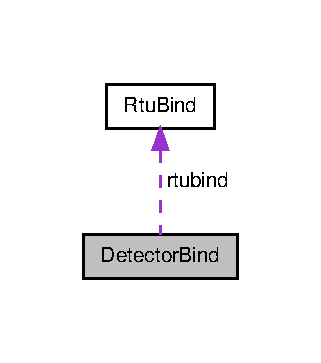
\includegraphics[width=154pt]{structDetectorBind__coll__graph}
\end{center}
\end{figure}
\subsection*{Data Fields}
\begin{DoxyCompactItemize}
\item 
\hyperlink{base_8h_a60cf7b3c038ce37a50796e8eaddf0b5f}{Uint32} \hyperlink{structDetectorBind_aafe967553a211b4b4659d5eb8503f01a}{hostadd}
\item 
\hyperlink{base_8h_a60cf7b3c038ce37a50796e8eaddf0b5f}{Uint32} \hyperlink{structDetectorBind_ac36a0d856c55e3567781683860435cdd}{rtuadd}
\item 
\hyperlink{base_8h_af84840501dec18061d18a68c162a8fa2}{Uint8} \hyperlink{structDetectorBind_af1ee9714c6d13cb58952b8ac210de246}{level}
\begin{DoxyCompactList}\small\item\em 联动级数 \end{DoxyCompactList}\item 
\hyperlink{base_8h_af84840501dec18061d18a68c162a8fa2}{Uint8} \hyperlink{structDetectorBind_aeb689d428cfe88f8f3f1402bf7f56e2e}{bind\-\_\-num}
\begin{DoxyCompactList}\small\item\em 绑定设备或情景数 \end{DoxyCompactList}\item 
\hyperlink{structRtuBind}{Rtu\-Bind} $\ast$ \hyperlink{structDetectorBind_a051da44e061843becfc64dd40e8a2d75}{rtubind}
\begin{DoxyCompactList}\small\item\em 绑定的操作信息 \end{DoxyCompactList}\end{DoxyCompactItemize}


\subsection{Detailed Description}
传感器联动绑定 结构体 

\subsection{Field Documentation}
\hypertarget{structDetectorBind_aeb689d428cfe88f8f3f1402bf7f56e2e}{\index{Detector\-Bind@{Detector\-Bind}!bind\-\_\-num@{bind\-\_\-num}}
\index{bind\-\_\-num@{bind\-\_\-num}!DetectorBind@{Detector\-Bind}}
\subsubsection[{bind\-\_\-num}]{\setlength{\rightskip}{0pt plus 5cm}{\bf Uint8} Detector\-Bind\-::bind\-\_\-num}}\label{structDetectorBind_aeb689d428cfe88f8f3f1402bf7f56e2e}


绑定设备或情景数 



Referenced by update\-\_\-db\-\_\-detectorbind().

\hypertarget{structDetectorBind_aafe967553a211b4b4659d5eb8503f01a}{\index{Detector\-Bind@{Detector\-Bind}!hostadd@{hostadd}}
\index{hostadd@{hostadd}!DetectorBind@{Detector\-Bind}}
\subsubsection[{hostadd}]{\setlength{\rightskip}{0pt plus 5cm}{\bf Uint32} Detector\-Bind\-::hostadd}}\label{structDetectorBind_aafe967553a211b4b4659d5eb8503f01a}


Referenced by update\-\_\-db\-\_\-detectorbind().

\hypertarget{structDetectorBind_af1ee9714c6d13cb58952b8ac210de246}{\index{Detector\-Bind@{Detector\-Bind}!level@{level}}
\index{level@{level}!DetectorBind@{Detector\-Bind}}
\subsubsection[{level}]{\setlength{\rightskip}{0pt plus 5cm}{\bf Uint8} Detector\-Bind\-::level}}\label{structDetectorBind_af1ee9714c6d13cb58952b8ac210de246}


联动级数 



Referenced by update\-\_\-db\-\_\-detectorbind().

\hypertarget{structDetectorBind_ac36a0d856c55e3567781683860435cdd}{\index{Detector\-Bind@{Detector\-Bind}!rtuadd@{rtuadd}}
\index{rtuadd@{rtuadd}!DetectorBind@{Detector\-Bind}}
\subsubsection[{rtuadd}]{\setlength{\rightskip}{0pt plus 5cm}{\bf Uint32} Detector\-Bind\-::rtuadd}}\label{structDetectorBind_ac36a0d856c55e3567781683860435cdd}


Referenced by update\-\_\-db\-\_\-detectorbind().

\hypertarget{structDetectorBind_a051da44e061843becfc64dd40e8a2d75}{\index{Detector\-Bind@{Detector\-Bind}!rtubind@{rtubind}}
\index{rtubind@{rtubind}!DetectorBind@{Detector\-Bind}}
\subsubsection[{rtubind}]{\setlength{\rightskip}{0pt plus 5cm}{\bf Rtu\-Bind}$\ast$ Detector\-Bind\-::rtubind}}\label{structDetectorBind_a051da44e061843becfc64dd40e8a2d75}


绑定的操作信息 



Referenced by update\-\_\-db\-\_\-detectorbind().



The documentation for this struct was generated from the following file\-:\begin{DoxyCompactItemize}
\item 
\hyperlink{dbbase_8h}{dbbase.\-h}\end{DoxyCompactItemize}

\hypertarget{structDetectorInfo}{\section{Detector\-Info Struct Reference}
\label{structDetectorInfo}\index{Detector\-Info@{Detector\-Info}}
}


{\ttfamily \#include $<$dbbase.\-h$>$}

\subsection*{Data Fields}
\begin{DoxyCompactItemize}
\item 
\hyperlink{base_8h_a60cf7b3c038ce37a50796e8eaddf0b5f}{Uint32} \hyperlink{structDetectorInfo_a413c1a19e7600530e457efbf839df865}{val} \mbox{[}3\mbox{]}
\item 
\hyperlink{base_8h_a60cf7b3c038ce37a50796e8eaddf0b5f}{Uint32} \hyperlink{structDetectorInfo_a97a917f0d89a2aef284980b3c5c5ea7a}{flag}
\item 
\hyperlink{base_8h_a60cf7b3c038ce37a50796e8eaddf0b5f}{Uint32} \hyperlink{structDetectorInfo_a7022303e238f95e44dbd3eea3a690270}{downval}
\item 
\hyperlink{base_8h_a60cf7b3c038ce37a50796e8eaddf0b5f}{Uint32} \hyperlink{structDetectorInfo_adb7255552b8dfb9eb1506fdd8d6c8105}{upval}
\end{DoxyCompactItemize}


\subsection{Detailed Description}
传感器设备尾部信息 

\subsection{Field Documentation}
\hypertarget{structDetectorInfo_a7022303e238f95e44dbd3eea3a690270}{\index{Detector\-Info@{Detector\-Info}!downval@{downval}}
\index{downval@{downval}!DetectorInfo@{Detector\-Info}}
\subsubsection[{downval}]{\setlength{\rightskip}{0pt plus 5cm}{\bf Uint32} Detector\-Info\-::downval}}\label{structDetectorInfo_a7022303e238f95e44dbd3eea3a690270}


Referenced by update\-\_\-db\-\_\-detectorrtu().

\hypertarget{structDetectorInfo_a97a917f0d89a2aef284980b3c5c5ea7a}{\index{Detector\-Info@{Detector\-Info}!flag@{flag}}
\index{flag@{flag}!DetectorInfo@{Detector\-Info}}
\subsubsection[{flag}]{\setlength{\rightskip}{0pt plus 5cm}{\bf Uint32} Detector\-Info\-::flag}}\label{structDetectorInfo_a97a917f0d89a2aef284980b3c5c5ea7a}


Referenced by update\-\_\-db\-\_\-detectorrtu().

\hypertarget{structDetectorInfo_adb7255552b8dfb9eb1506fdd8d6c8105}{\index{Detector\-Info@{Detector\-Info}!upval@{upval}}
\index{upval@{upval}!DetectorInfo@{Detector\-Info}}
\subsubsection[{upval}]{\setlength{\rightskip}{0pt plus 5cm}{\bf Uint32} Detector\-Info\-::upval}}\label{structDetectorInfo_adb7255552b8dfb9eb1506fdd8d6c8105}


Referenced by update\-\_\-db\-\_\-detectorrtu().

\hypertarget{structDetectorInfo_a413c1a19e7600530e457efbf839df865}{\index{Detector\-Info@{Detector\-Info}!val@{val}}
\index{val@{val}!DetectorInfo@{Detector\-Info}}
\subsubsection[{val}]{\setlength{\rightskip}{0pt plus 5cm}{\bf Uint32} Detector\-Info\-::val\mbox{[}3\mbox{]}}}\label{structDetectorInfo_a413c1a19e7600530e457efbf839df865}


Referenced by update\-\_\-db\-\_\-detectorrtu().



The documentation for this struct was generated from the following file\-:\begin{DoxyCompactItemize}
\item 
\hyperlink{dbbase_8h}{dbbase.\-h}\end{DoxyCompactItemize}

\hypertarget{structDetectorRtu}{\section{Detector\-Rtu Struct Reference}
\label{structDetectorRtu}\index{Detector\-Rtu@{Detector\-Rtu}}
}


{\ttfamily \#include $<$dbbase.\-h$>$}



Collaboration diagram for Detector\-Rtu\-:\nopagebreak
\begin{figure}[H]
\begin{center}
\leavevmode
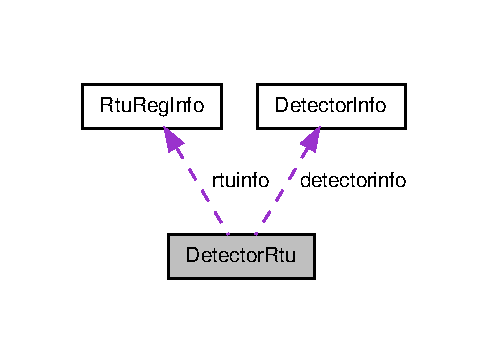
\includegraphics[width=236pt]{structDetectorRtu__coll__graph}
\end{center}
\end{figure}
\subsection*{Data Fields}
\begin{DoxyCompactItemize}
\item 
\hyperlink{structRtuRegInfo}{Rtu\-Reg\-Info} \hyperlink{structDetectorRtu_a0cc8bb5f4b4f63380fabd7d7e6c82849}{rtuinfo}
\begin{DoxyCompactList}\small\item\em 设备头信息 \end{DoxyCompactList}\item 
\hyperlink{base_8h_af84840501dec18061d18a68c162a8fa2}{Uint8} \hyperlink{structDetectorRtu_a0b30b25acdbd4d7dc62ac9b50daf64f0}{valtype}
\item 
\hyperlink{structDetectorInfo}{Detector\-Info} \hyperlink{structDetectorRtu_a2d98ee3ad1fe130208268ee868dc5dab}{detectorinfo}
\end{DoxyCompactItemize}


\subsection{Detailed Description}
传感器设备 结构体 

\subsection{Field Documentation}
\hypertarget{structDetectorRtu_a2d98ee3ad1fe130208268ee868dc5dab}{\index{Detector\-Rtu@{Detector\-Rtu}!detectorinfo@{detectorinfo}}
\index{detectorinfo@{detectorinfo}!DetectorRtu@{Detector\-Rtu}}
\subsubsection[{detectorinfo}]{\setlength{\rightskip}{0pt plus 5cm}{\bf Detector\-Info} Detector\-Rtu\-::detectorinfo}}\label{structDetectorRtu_a2d98ee3ad1fe130208268ee868dc5dab}


Referenced by update\-\_\-db\-\_\-detectorrtu().

\hypertarget{structDetectorRtu_a0cc8bb5f4b4f63380fabd7d7e6c82849}{\index{Detector\-Rtu@{Detector\-Rtu}!rtuinfo@{rtuinfo}}
\index{rtuinfo@{rtuinfo}!DetectorRtu@{Detector\-Rtu}}
\subsubsection[{rtuinfo}]{\setlength{\rightskip}{0pt plus 5cm}{\bf Rtu\-Reg\-Info} Detector\-Rtu\-::rtuinfo}}\label{structDetectorRtu_a0cc8bb5f4b4f63380fabd7d7e6c82849}


设备头信息 



Referenced by update\-\_\-db\-\_\-detectorrtu().

\hypertarget{structDetectorRtu_a0b30b25acdbd4d7dc62ac9b50daf64f0}{\index{Detector\-Rtu@{Detector\-Rtu}!valtype@{valtype}}
\index{valtype@{valtype}!DetectorRtu@{Detector\-Rtu}}
\subsubsection[{valtype}]{\setlength{\rightskip}{0pt plus 5cm}{\bf Uint8} Detector\-Rtu\-::valtype}}\label{structDetectorRtu_a0b30b25acdbd4d7dc62ac9b50daf64f0}


Referenced by update\-\_\-db\-\_\-detectorrtu().



The documentation for this struct was generated from the following file\-:\begin{DoxyCompactItemize}
\item 
\hyperlink{dbbase_8h}{dbbase.\-h}\end{DoxyCompactItemize}

\hypertarget{structExNativeRtu}{\section{Ex\-Native\-Rtu Struct Reference}
\label{structExNativeRtu}\index{Ex\-Native\-Rtu@{Ex\-Native\-Rtu}}
}


{\ttfamily \#include $<$dbbase.\-h$>$}



Collaboration diagram for Ex\-Native\-Rtu\-:\nopagebreak
\begin{figure}[H]
\begin{center}
\leavevmode
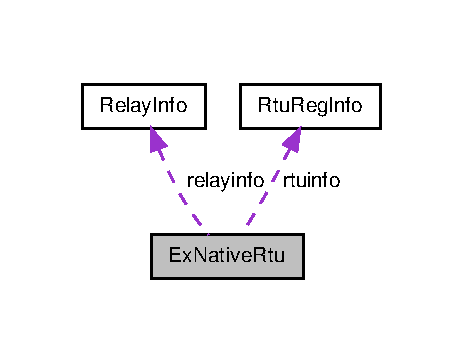
\includegraphics[width=222pt]{structExNativeRtu__coll__graph}
\end{center}
\end{figure}
\subsection*{Data Fields}
\begin{DoxyCompactItemize}
\item 
\hyperlink{structRtuRegInfo}{Rtu\-Reg\-Info} \hyperlink{structExNativeRtu_a880cf200ec393f75b6a72b3a47b8af88}{rtuinfo}
\begin{DoxyCompactList}\small\item\em 设备头信息 \end{DoxyCompactList}\item 
\hyperlink{structRelayInfo}{Relay\-Info} \hyperlink{structExNativeRtu_a8bff0a97f7771458d2ab36a2854d7247}{relayinfo} \mbox{[}5\mbox{]}
\end{DoxyCompactItemize}


\subsection{Detailed Description}
智能床 设备 

\subsection{Field Documentation}
\hypertarget{structExNativeRtu_a8bff0a97f7771458d2ab36a2854d7247}{\index{Ex\-Native\-Rtu@{Ex\-Native\-Rtu}!relayinfo@{relayinfo}}
\index{relayinfo@{relayinfo}!ExNativeRtu@{Ex\-Native\-Rtu}}
\subsubsection[{relayinfo}]{\setlength{\rightskip}{0pt plus 5cm}{\bf Relay\-Info} Ex\-Native\-Rtu\-::relayinfo\mbox{[}5\mbox{]}}}\label{structExNativeRtu_a8bff0a97f7771458d2ab36a2854d7247}


Referenced by update\-\_\-db\-\_\-exnativertu().

\hypertarget{structExNativeRtu_a880cf200ec393f75b6a72b3a47b8af88}{\index{Ex\-Native\-Rtu@{Ex\-Native\-Rtu}!rtuinfo@{rtuinfo}}
\index{rtuinfo@{rtuinfo}!ExNativeRtu@{Ex\-Native\-Rtu}}
\subsubsection[{rtuinfo}]{\setlength{\rightskip}{0pt plus 5cm}{\bf Rtu\-Reg\-Info} Ex\-Native\-Rtu\-::rtuinfo}}\label{structExNativeRtu_a880cf200ec393f75b6a72b3a47b8af88}


设备头信息 



Referenced by update\-\_\-db\-\_\-exnativertu().



The documentation for this struct was generated from the following file\-:\begin{DoxyCompactItemize}
\item 
\hyperlink{dbbase_8h}{dbbase.\-h}\end{DoxyCompactItemize}

\hypertarget{structHostMan}{\section{Host\-Man Struct Reference}
\label{structHostMan}\index{Host\-Man@{Host\-Man}}
}


{\ttfamily \#include $<$dbbase.\-h$>$}

\subsection*{Data Fields}
\begin{DoxyCompactItemize}
\item 
char \hyperlink{structHostMan_a1441529ae42ac0b02704431e41f5b5c3}{oldname} \mbox{[}\hyperlink{dbbase_8h_a6c4647395896246d6710ba980c31666c}{M\-A\-X\-\_\-\-U\-S\-E\-R\-N\-A\-M\-E\-\_\-\-L\-E\-N}\mbox{]}
\begin{DoxyCompactList}\small\item\em 原主机名 \end{DoxyCompactList}\item 
char \hyperlink{structHostMan_a94f32dd3715b3069fa469ca3ea5ea1e7}{oldpwd} \mbox{[}\hyperlink{dbbase_8h_ae9169c3fda2dfecbb7a13e394a69e5be}{M\-A\-X\-\_\-\-P\-A\-S\-S\-W\-O\-R\-D\-\_\-\-L\-E\-N}\mbox{]}
\begin{DoxyCompactList}\small\item\em 原主机密码 \end{DoxyCompactList}\item 
char \hyperlink{structHostMan_a51767ec848f109bccbddb87550ff88d9}{newname} \mbox{[}\hyperlink{dbbase_8h_a6c4647395896246d6710ba980c31666c}{M\-A\-X\-\_\-\-U\-S\-E\-R\-N\-A\-M\-E\-\_\-\-L\-E\-N}\mbox{]}
\begin{DoxyCompactList}\small\item\em 新主机名 \end{DoxyCompactList}\item 
char \hyperlink{structHostMan_a6f5cb28d8740dae24ee076d6cd2fb63e}{newpwd} \mbox{[}\hyperlink{dbbase_8h_ae9169c3fda2dfecbb7a13e394a69e5be}{M\-A\-X\-\_\-\-P\-A\-S\-S\-W\-O\-R\-D\-\_\-\-L\-E\-N}\mbox{]}
\begin{DoxyCompactList}\small\item\em 新主机密码 \end{DoxyCompactList}\end{DoxyCompactItemize}


\subsection{Detailed Description}
主机用户修改 

\subsection{Field Documentation}
\hypertarget{structHostMan_a51767ec848f109bccbddb87550ff88d9}{\index{Host\-Man@{Host\-Man}!newname@{newname}}
\index{newname@{newname}!HostMan@{Host\-Man}}
\subsubsection[{newname}]{\setlength{\rightskip}{0pt plus 5cm}char Host\-Man\-::newname\mbox{[}{\bf M\-A\-X\-\_\-\-U\-S\-E\-R\-N\-A\-M\-E\-\_\-\-L\-E\-N}\mbox{]}}}\label{structHostMan_a51767ec848f109bccbddb87550ff88d9}


新主机名 



Referenced by update\-\_\-db\-\_\-hostname().

\hypertarget{structHostMan_a6f5cb28d8740dae24ee076d6cd2fb63e}{\index{Host\-Man@{Host\-Man}!newpwd@{newpwd}}
\index{newpwd@{newpwd}!HostMan@{Host\-Man}}
\subsubsection[{newpwd}]{\setlength{\rightskip}{0pt plus 5cm}char Host\-Man\-::newpwd\mbox{[}{\bf M\-A\-X\-\_\-\-P\-A\-S\-S\-W\-O\-R\-D\-\_\-\-L\-E\-N}\mbox{]}}}\label{structHostMan_a6f5cb28d8740dae24ee076d6cd2fb63e}


新主机密码 



Referenced by update\-\_\-db\-\_\-hostname().

\hypertarget{structHostMan_a1441529ae42ac0b02704431e41f5b5c3}{\index{Host\-Man@{Host\-Man}!oldname@{oldname}}
\index{oldname@{oldname}!HostMan@{Host\-Man}}
\subsubsection[{oldname}]{\setlength{\rightskip}{0pt plus 5cm}char Host\-Man\-::oldname\mbox{[}{\bf M\-A\-X\-\_\-\-U\-S\-E\-R\-N\-A\-M\-E\-\_\-\-L\-E\-N}\mbox{]}}}\label{structHostMan_a1441529ae42ac0b02704431e41f5b5c3}


原主机名 



Referenced by update\-\_\-db\-\_\-hostname().

\hypertarget{structHostMan_a94f32dd3715b3069fa469ca3ea5ea1e7}{\index{Host\-Man@{Host\-Man}!oldpwd@{oldpwd}}
\index{oldpwd@{oldpwd}!HostMan@{Host\-Man}}
\subsubsection[{oldpwd}]{\setlength{\rightskip}{0pt plus 5cm}char Host\-Man\-::oldpwd\mbox{[}{\bf M\-A\-X\-\_\-\-P\-A\-S\-S\-W\-O\-R\-D\-\_\-\-L\-E\-N}\mbox{]}}}\label{structHostMan_a94f32dd3715b3069fa469ca3ea5ea1e7}


原主机密码 



Referenced by update\-\_\-db\-\_\-hostname().



The documentation for this struct was generated from the following file\-:\begin{DoxyCompactItemize}
\item 
\hyperlink{dbbase_8h}{dbbase.\-h}\end{DoxyCompactItemize}

\hypertarget{structHostRegInfo}{\section{Host\-Reg\-Info Struct Reference}
\label{structHostRegInfo}\index{Host\-Reg\-Info@{Host\-Reg\-Info}}
}


{\ttfamily \#include $<$dbbase.\-h$>$}

\subsection*{Data Fields}
\begin{DoxyCompactItemize}
\item 
char \hyperlink{structHostRegInfo_abaad6f194144e79d59f3f50e7eb078af}{hostname} \mbox{[}\hyperlink{dbbase_8h_a6c4647395896246d6710ba980c31666c}{M\-A\-X\-\_\-\-U\-S\-E\-R\-N\-A\-M\-E\-\_\-\-L\-E\-N}\mbox{]}
\begin{DoxyCompactList}\small\item\em 主机名 \end{DoxyCompactList}\item 
\hyperlink{base_8h_a60cf7b3c038ce37a50796e8eaddf0b5f}{Uint32} \hyperlink{structHostRegInfo_a3b304abdc867e6ac1d510ccec832e844}{hostadd}
\begin{DoxyCompactList}\small\item\em 主机地址 \end{DoxyCompactList}\item 
char \hyperlink{structHostRegInfo_a19bb5479f6700b3eafb505d4cb16bf11}{hostpwd} \mbox{[}\hyperlink{dbbase_8h_ae9169c3fda2dfecbb7a13e394a69e5be}{M\-A\-X\-\_\-\-P\-A\-S\-S\-W\-O\-R\-D\-\_\-\-L\-E\-N}\mbox{]}
\begin{DoxyCompactList}\small\item\em 主机密码 \end{DoxyCompactList}\item 
char \hyperlink{structHostRegInfo_aae80f759cd5835a9b695f2707a1b60e4}{hostregtime} \mbox{[}30\mbox{]}
\begin{DoxyCompactList}\small\item\em 注册时间 \end{DoxyCompactList}\item 
\hyperlink{dbbase_8h_afec5109c9a49125c493619b015292bb0}{Rtustatus} \hyperlink{structHostRegInfo_a6f478e420e2736db1408a6dcd4927e8f}{hoststate}
\begin{DoxyCompactList}\small\item\em 注册状态 \end{DoxyCompactList}\item 
\hyperlink{base_8h_a60cf7b3c038ce37a50796e8eaddf0b5f}{Uint32} \hyperlink{structHostRegInfo_ac2a4fc92c30a444b52fca1fd0589a027}{hostip}
\begin{DoxyCompactList}\small\item\em 主机 ip : bytes\mbox{[}3\-:2\-:1\-:0\mbox{]} \end{DoxyCompactList}\item 
char \hyperlink{structHostRegInfo_a20b46c33f6aed2a9d4e11ae3f2ec2cee}{lastcomtime} \mbox{[}30\mbox{]}
\begin{DoxyCompactList}\small\item\em void$\ast$ \end{DoxyCompactList}\end{DoxyCompactItemize}


\subsection{Detailed Description}
主机注册结构体 

\subsection{Field Documentation}
\hypertarget{structHostRegInfo_a3b304abdc867e6ac1d510ccec832e844}{\index{Host\-Reg\-Info@{Host\-Reg\-Info}!hostadd@{hostadd}}
\index{hostadd@{hostadd}!HostRegInfo@{Host\-Reg\-Info}}
\subsubsection[{hostadd}]{\setlength{\rightskip}{0pt plus 5cm}{\bf Uint32} Host\-Reg\-Info\-::hostadd}}\label{structHostRegInfo_a3b304abdc867e6ac1d510ccec832e844}


主机地址 



Referenced by insert\-\_\-db\-\_\-host(), and select\-\_\-db\-\_\-hostinfo().

\hypertarget{structHostRegInfo_ac2a4fc92c30a444b52fca1fd0589a027}{\index{Host\-Reg\-Info@{Host\-Reg\-Info}!hostip@{hostip}}
\index{hostip@{hostip}!HostRegInfo@{Host\-Reg\-Info}}
\subsubsection[{hostip}]{\setlength{\rightskip}{0pt plus 5cm}{\bf Uint32} Host\-Reg\-Info\-::hostip}}\label{structHostRegInfo_ac2a4fc92c30a444b52fca1fd0589a027}


主机 ip : bytes\mbox{[}3\-:2\-:1\-:0\mbox{]} 



Referenced by insert\-\_\-db\-\_\-host(), select\-\_\-db\-\_\-hostinfo(), and update\-\_\-db\-\_\-host().

\hypertarget{structHostRegInfo_abaad6f194144e79d59f3f50e7eb078af}{\index{Host\-Reg\-Info@{Host\-Reg\-Info}!hostname@{hostname}}
\index{hostname@{hostname}!HostRegInfo@{Host\-Reg\-Info}}
\subsubsection[{hostname}]{\setlength{\rightskip}{0pt plus 5cm}char Host\-Reg\-Info\-::hostname\mbox{[}{\bf M\-A\-X\-\_\-\-U\-S\-E\-R\-N\-A\-M\-E\-\_\-\-L\-E\-N}\mbox{]}}}\label{structHostRegInfo_abaad6f194144e79d59f3f50e7eb078af}


主机名 



Referenced by insert\-\_\-db\-\_\-host(), and update\-\_\-db\-\_\-host().

\hypertarget{structHostRegInfo_a19bb5479f6700b3eafb505d4cb16bf11}{\index{Host\-Reg\-Info@{Host\-Reg\-Info}!hostpwd@{hostpwd}}
\index{hostpwd@{hostpwd}!HostRegInfo@{Host\-Reg\-Info}}
\subsubsection[{hostpwd}]{\setlength{\rightskip}{0pt plus 5cm}char Host\-Reg\-Info\-::hostpwd\mbox{[}{\bf M\-A\-X\-\_\-\-P\-A\-S\-S\-W\-O\-R\-D\-\_\-\-L\-E\-N}\mbox{]}}}\label{structHostRegInfo_a19bb5479f6700b3eafb505d4cb16bf11}


主机密码 



Referenced by insert\-\_\-db\-\_\-host(), and select\-\_\-db\-\_\-hostinfo().

\hypertarget{structHostRegInfo_aae80f759cd5835a9b695f2707a1b60e4}{\index{Host\-Reg\-Info@{Host\-Reg\-Info}!hostregtime@{hostregtime}}
\index{hostregtime@{hostregtime}!HostRegInfo@{Host\-Reg\-Info}}
\subsubsection[{hostregtime}]{\setlength{\rightskip}{0pt plus 5cm}char Host\-Reg\-Info\-::hostregtime\mbox{[}30\mbox{]}}}\label{structHostRegInfo_aae80f759cd5835a9b695f2707a1b60e4}


注册时间 



Referenced by insert\-\_\-db\-\_\-host().

\hypertarget{structHostRegInfo_a6f478e420e2736db1408a6dcd4927e8f}{\index{Host\-Reg\-Info@{Host\-Reg\-Info}!hoststate@{hoststate}}
\index{hoststate@{hoststate}!HostRegInfo@{Host\-Reg\-Info}}
\subsubsection[{hoststate}]{\setlength{\rightskip}{0pt plus 5cm}{\bf Rtustatus} Host\-Reg\-Info\-::hoststate}}\label{structHostRegInfo_a6f478e420e2736db1408a6dcd4927e8f}


注册状态 



Referenced by select\-\_\-db\-\_\-hostinfo().

\hypertarget{structHostRegInfo_a20b46c33f6aed2a9d4e11ae3f2ec2cee}{\index{Host\-Reg\-Info@{Host\-Reg\-Info}!lastcomtime@{lastcomtime}}
\index{lastcomtime@{lastcomtime}!HostRegInfo@{Host\-Reg\-Info}}
\subsubsection[{lastcomtime}]{\setlength{\rightskip}{0pt plus 5cm}char Host\-Reg\-Info\-::lastcomtime\mbox{[}30\mbox{]}}}\label{structHostRegInfo_a20b46c33f6aed2a9d4e11ae3f2ec2cee}


void$\ast$ 

最近通信时间 

Referenced by insert\-\_\-db\-\_\-host(), and select\-\_\-db\-\_\-hostinfo().



The documentation for this struct was generated from the following file\-:\begin{DoxyCompactItemize}
\item 
\hyperlink{dbbase_8h}{dbbase.\-h}\end{DoxyCompactItemize}

\hypertarget{structMysqlConInfo}{\section{Mysql\-Con\-Info Struct Reference}
\label{structMysqlConInfo}\index{Mysql\-Con\-Info@{Mysql\-Con\-Info}}
}


{\ttfamily \#include $<$dbbase.\-h$>$}

\subsection*{Data Fields}
\begin{DoxyCompactItemize}
\item 
char \hyperlink{structMysqlConInfo_a9382fdbd16ae319c1ad0a76b2362bd46}{hostname} \mbox{[}\hyperlink{dbbase_8h_a06a9cf374e83dcac0620e5095f79234e}{M\-A\-X\-\_\-\-S\-Q\-L\-N\-A\-M\-E\-\_\-\-L\-E\-N}\mbox{]}
\begin{DoxyCompactList}\small\item\em 数据库主机名 \end{DoxyCompactList}\item 
char \hyperlink{structMysqlConInfo_a2753d5c9d81aba6435ad503db842775d}{username} \mbox{[}\hyperlink{dbbase_8h_a998c6ce37817a02bf23a1a2c6fd15cb0}{M\-A\-X\-\_\-\-S\-Q\-L\-U\-S\-E\-R\-N\-A\-M\-E\-\_\-\-L\-E\-N}\mbox{]}
\begin{DoxyCompactList}\small\item\em 数据库用户名 \end{DoxyCompactList}\item 
char \hyperlink{structMysqlConInfo_a429e8aae687715a9ec374435c026f939}{password} \mbox{[}\hyperlink{dbbase_8h_ae5cf418bda87e648ae461cfbca7e2f8e}{M\-A\-X\-\_\-\-S\-Q\-L\-P\-A\-S\-S\-W\-D\-\_\-\-L\-E\-N}\mbox{]}
\begin{DoxyCompactList}\small\item\em 数据库密码 \end{DoxyCompactList}\item 
char \hyperlink{structMysqlConInfo_a82550a94a5bc9800f388752f01964c1c}{dbname} \mbox{[}\hyperlink{dbbase_8h_a06a9cf374e83dcac0620e5095f79234e}{M\-A\-X\-\_\-\-S\-Q\-L\-N\-A\-M\-E\-\_\-\-L\-E\-N}\mbox{]}
\begin{DoxyCompactList}\small\item\em 数据库名 \end{DoxyCompactList}\end{DoxyCompactItemize}


\subsection{Detailed Description}
mysql 连接结构体 

\subsection{Field Documentation}
\hypertarget{structMysqlConInfo_a82550a94a5bc9800f388752f01964c1c}{\index{Mysql\-Con\-Info@{Mysql\-Con\-Info}!dbname@{dbname}}
\index{dbname@{dbname}!MysqlConInfo@{Mysql\-Con\-Info}}
\subsubsection[{dbname}]{\setlength{\rightskip}{0pt plus 5cm}char Mysql\-Con\-Info\-::dbname\mbox{[}{\bf M\-A\-X\-\_\-\-S\-Q\-L\-N\-A\-M\-E\-\_\-\-L\-E\-N}\mbox{]}}}\label{structMysqlConInfo_a82550a94a5bc9800f388752f01964c1c}


数据库名 



Referenced by init\-\_\-mysql().

\hypertarget{structMysqlConInfo_a9382fdbd16ae319c1ad0a76b2362bd46}{\index{Mysql\-Con\-Info@{Mysql\-Con\-Info}!hostname@{hostname}}
\index{hostname@{hostname}!MysqlConInfo@{Mysql\-Con\-Info}}
\subsubsection[{hostname}]{\setlength{\rightskip}{0pt plus 5cm}char Mysql\-Con\-Info\-::hostname\mbox{[}{\bf M\-A\-X\-\_\-\-S\-Q\-L\-N\-A\-M\-E\-\_\-\-L\-E\-N}\mbox{]}}}\label{structMysqlConInfo_a9382fdbd16ae319c1ad0a76b2362bd46}


数据库主机名 



Referenced by init\-\_\-mysql().

\hypertarget{structMysqlConInfo_a429e8aae687715a9ec374435c026f939}{\index{Mysql\-Con\-Info@{Mysql\-Con\-Info}!password@{password}}
\index{password@{password}!MysqlConInfo@{Mysql\-Con\-Info}}
\subsubsection[{password}]{\setlength{\rightskip}{0pt plus 5cm}char Mysql\-Con\-Info\-::password\mbox{[}{\bf M\-A\-X\-\_\-\-S\-Q\-L\-P\-A\-S\-S\-W\-D\-\_\-\-L\-E\-N}\mbox{]}}}\label{structMysqlConInfo_a429e8aae687715a9ec374435c026f939}


数据库密码 



Referenced by init\-\_\-mysql().

\hypertarget{structMysqlConInfo_a2753d5c9d81aba6435ad503db842775d}{\index{Mysql\-Con\-Info@{Mysql\-Con\-Info}!username@{username}}
\index{username@{username}!MysqlConInfo@{Mysql\-Con\-Info}}
\subsubsection[{username}]{\setlength{\rightskip}{0pt plus 5cm}char Mysql\-Con\-Info\-::username\mbox{[}{\bf M\-A\-X\-\_\-\-S\-Q\-L\-U\-S\-E\-R\-N\-A\-M\-E\-\_\-\-L\-E\-N}\mbox{]}}}\label{structMysqlConInfo_a2753d5c9d81aba6435ad503db842775d}


数据库用户名 



Referenced by init\-\_\-mysql().



The documentation for this struct was generated from the following file\-:\begin{DoxyCompactItemize}
\item 
\hyperlink{dbbase_8h}{dbbase.\-h}\end{DoxyCompactItemize}

\hypertarget{structNativeRtuInfo}{\section{Native\-Rtu\-Info Struct Reference}
\label{structNativeRtuInfo}\index{Native\-Rtu\-Info@{Native\-Rtu\-Info}}
}


{\ttfamily \#include $<$dbbase.\-h$>$}



Collaboration diagram for Native\-Rtu\-Info\-:\nopagebreak
\begin{figure}[H]
\begin{center}
\leavevmode
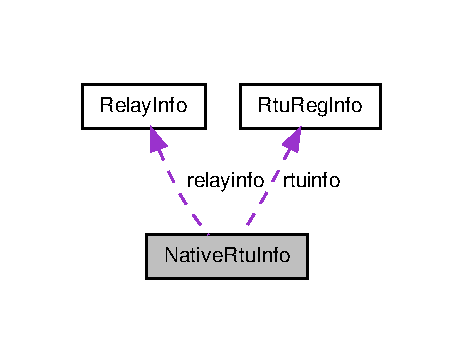
\includegraphics[width=222pt]{structNativeRtuInfo__coll__graph}
\end{center}
\end{figure}
\subsection*{Data Fields}
\begin{DoxyCompactItemize}
\item 
\hyperlink{structRtuRegInfo}{Rtu\-Reg\-Info} \hyperlink{structNativeRtuInfo_aadeca7477bda9a54e67e8b6409998197}{rtuinfo}
\begin{DoxyCompactList}\small\item\em 设备头信息 \end{DoxyCompactList}\item 
\hyperlink{base_8h_ae9f2e1f80fbd243687a04febbf590e13}{Uint16} \hyperlink{structNativeRtuInfo_ae673b07d8c87e05626830f4e1b813f99}{bind\-\_\-num}
\begin{DoxyCompactList}\small\item\em 继电器绑定负载 是传入 绑定数目 \end{DoxyCompactList}\item 
\hyperlink{structRelayInfo}{Relay\-Info} \hyperlink{structNativeRtuInfo_ad9f9b53a53485f4e89e85dbc510348b6}{relayinfo} \mbox{[}4\mbox{]}
\begin{DoxyCompactList}\small\item\em 继电器负载 和控制value \end{DoxyCompactList}\end{DoxyCompactItemize}


\subsection{Detailed Description}
常规设备结构体 

\subsection{Field Documentation}
\hypertarget{structNativeRtuInfo_ae673b07d8c87e05626830f4e1b813f99}{\index{Native\-Rtu\-Info@{Native\-Rtu\-Info}!bind\-\_\-num@{bind\-\_\-num}}
\index{bind\-\_\-num@{bind\-\_\-num}!NativeRtuInfo@{Native\-Rtu\-Info}}
\subsubsection[{bind\-\_\-num}]{\setlength{\rightskip}{0pt plus 5cm}{\bf Uint16} Native\-Rtu\-Info\-::bind\-\_\-num}}\label{structNativeRtuInfo_ae673b07d8c87e05626830f4e1b813f99}


继电器绑定负载 是传入 绑定数目 



Referenced by update\-\_\-db\-\_\-nativertu().

\hypertarget{structNativeRtuInfo_ad9f9b53a53485f4e89e85dbc510348b6}{\index{Native\-Rtu\-Info@{Native\-Rtu\-Info}!relayinfo@{relayinfo}}
\index{relayinfo@{relayinfo}!NativeRtuInfo@{Native\-Rtu\-Info}}
\subsubsection[{relayinfo}]{\setlength{\rightskip}{0pt plus 5cm}{\bf Relay\-Info} Native\-Rtu\-Info\-::relayinfo\mbox{[}4\mbox{]}}}\label{structNativeRtuInfo_ad9f9b53a53485f4e89e85dbc510348b6}


继电器负载 和控制value 



Referenced by update\-\_\-db\-\_\-nativertu().

\hypertarget{structNativeRtuInfo_aadeca7477bda9a54e67e8b6409998197}{\index{Native\-Rtu\-Info@{Native\-Rtu\-Info}!rtuinfo@{rtuinfo}}
\index{rtuinfo@{rtuinfo}!NativeRtuInfo@{Native\-Rtu\-Info}}
\subsubsection[{rtuinfo}]{\setlength{\rightskip}{0pt plus 5cm}{\bf Rtu\-Reg\-Info} Native\-Rtu\-Info\-::rtuinfo}}\label{structNativeRtuInfo_aadeca7477bda9a54e67e8b6409998197}


设备头信息 



Referenced by update\-\_\-db\-\_\-nativertu().



The documentation for this struct was generated from the following file\-:\begin{DoxyCompactItemize}
\item 
\hyperlink{dbbase_8h}{dbbase.\-h}\end{DoxyCompactItemize}

\hypertarget{structRelayInfo}{\section{Relay\-Info Struct Reference}
\label{structRelayInfo}\index{Relay\-Info@{Relay\-Info}}
}


{\ttfamily \#include $<$dbbase.\-h$>$}

\subsection*{Data Fields}
\begin{DoxyCompactItemize}
\item 
\hyperlink{base_8h_ae9f2e1f80fbd243687a04febbf590e13}{Uint16} \hyperlink{structRelayInfo_a664b6fde886aa5ec22584d57805989ba}{id}
\begin{DoxyCompactList}\small\item\em 继电器序号 \end{DoxyCompactList}\item 
\hyperlink{base_8h_ae9f2e1f80fbd243687a04febbf590e13}{Uint16} \hyperlink{structRelayInfo_a1f47e160c39504214a046234af05ff26}{type}
\begin{DoxyCompactList}\small\item\em 负载类型 \end{DoxyCompactList}\item 
\hyperlink{base_8h_a60cf7b3c038ce37a50796e8eaddf0b5f}{Uint32} \hyperlink{structRelayInfo_a4dc7bba5c5dd2ee1ff7172bae972936f}{val}
\begin{DoxyCompactList}\small\item\em 负载value \end{DoxyCompactList}\item 
char \hyperlink{structRelayInfo_a560c82273099e57eee9c873de36ec4d9}{name} \mbox{[}32\mbox{]}
\begin{DoxyCompactList}\small\item\em 负载名称 \end{DoxyCompactList}\item 
char \hyperlink{structRelayInfo_a9135480956d928283d45f91635aeefa1}{path} \mbox{[}32\mbox{]}
\begin{DoxyCompactList}\small\item\em 负载路径 \end{DoxyCompactList}\end{DoxyCompactItemize}


\subsection{Detailed Description}
常规设备尾部控制部分 

\subsection{Field Documentation}
\hypertarget{structRelayInfo_a664b6fde886aa5ec22584d57805989ba}{\index{Relay\-Info@{Relay\-Info}!id@{id}}
\index{id@{id}!RelayInfo@{Relay\-Info}}
\subsubsection[{id}]{\setlength{\rightskip}{0pt plus 5cm}{\bf Uint16} Relay\-Info\-::id}}\label{structRelayInfo_a664b6fde886aa5ec22584d57805989ba}


继电器序号 



Referenced by update\-\_\-db\-\_\-nativertu().

\hypertarget{structRelayInfo_a560c82273099e57eee9c873de36ec4d9}{\index{Relay\-Info@{Relay\-Info}!name@{name}}
\index{name@{name}!RelayInfo@{Relay\-Info}}
\subsubsection[{name}]{\setlength{\rightskip}{0pt plus 5cm}char Relay\-Info\-::name\mbox{[}32\mbox{]}}}\label{structRelayInfo_a560c82273099e57eee9c873de36ec4d9}


负载名称 



Referenced by update\-\_\-db\-\_\-nativertu().

\hypertarget{structRelayInfo_a9135480956d928283d45f91635aeefa1}{\index{Relay\-Info@{Relay\-Info}!path@{path}}
\index{path@{path}!RelayInfo@{Relay\-Info}}
\subsubsection[{path}]{\setlength{\rightskip}{0pt plus 5cm}char Relay\-Info\-::path\mbox{[}32\mbox{]}}}\label{structRelayInfo_a9135480956d928283d45f91635aeefa1}


负载路径 



Referenced by update\-\_\-db\-\_\-nativertu().

\hypertarget{structRelayInfo_a1f47e160c39504214a046234af05ff26}{\index{Relay\-Info@{Relay\-Info}!type@{type}}
\index{type@{type}!RelayInfo@{Relay\-Info}}
\subsubsection[{type}]{\setlength{\rightskip}{0pt plus 5cm}{\bf Uint16} Relay\-Info\-::type}}\label{structRelayInfo_a1f47e160c39504214a046234af05ff26}


负载类型 



Referenced by update\-\_\-db\-\_\-nativertu().

\hypertarget{structRelayInfo_a4dc7bba5c5dd2ee1ff7172bae972936f}{\index{Relay\-Info@{Relay\-Info}!val@{val}}
\index{val@{val}!RelayInfo@{Relay\-Info}}
\subsubsection[{val}]{\setlength{\rightskip}{0pt plus 5cm}{\bf Uint32} Relay\-Info\-::val}}\label{structRelayInfo_a4dc7bba5c5dd2ee1ff7172bae972936f}


负载value 



Referenced by update\-\_\-db\-\_\-exnativertu(), and update\-\_\-db\-\_\-nativertu().



The documentation for this struct was generated from the following file\-:\begin{DoxyCompactItemize}
\item 
\hyperlink{dbbase_8h}{dbbase.\-h}\end{DoxyCompactItemize}

\hypertarget{structRtuBind}{\section{Rtu\-Bind Struct Reference}
\label{structRtuBind}\index{Rtu\-Bind@{Rtu\-Bind}}
}


{\ttfamily \#include $<$dbbase.\-h$>$}

\subsection*{Data Fields}
\begin{DoxyCompactItemize}
\item 
\hyperlink{base_8h_ae9f2e1f80fbd243687a04febbf590e13}{Uint16} \hyperlink{structRtuBind_ab9f60247ea34410bf323084c15435d65}{type}
\begin{DoxyCompactList}\small\item\em 绑定类型 \end{DoxyCompactList}\item 
\hyperlink{base_8h_a60cf7b3c038ce37a50796e8eaddf0b5f}{Uint32} \hyperlink{structRtuBind_a68a5063b5ae740267f3d8d72f1400c6e}{add}
\begin{DoxyCompactList}\small\item\em 绑定设备/ 情景地址 \end{DoxyCompactList}\item 
\hyperlink{base_8h_a60cf7b3c038ce37a50796e8eaddf0b5f}{Uint32} \hyperlink{structRtuBind_ac466a6951df3423d75ab25ce3accede3}{oper}
\begin{DoxyCompactList}\small\item\em 绑定设备继电器1-\/4的操作 4个字节 \end{DoxyCompactList}\item 
\hyperlink{base_8h_a60cf7b3c038ce37a50796e8eaddf0b5f}{Uint32} \hyperlink{structRtuBind_aa231213efdd49f97effe6b5dc9f4a243}{delay}
\begin{DoxyCompactList}\small\item\em 延时 \end{DoxyCompactList}\end{DoxyCompactItemize}


\subsection{Detailed Description}
绑定的设备信息 

\subsection{Field Documentation}
\hypertarget{structRtuBind_a68a5063b5ae740267f3d8d72f1400c6e}{\index{Rtu\-Bind@{Rtu\-Bind}!add@{add}}
\index{add@{add}!RtuBind@{Rtu\-Bind}}
\subsubsection[{add}]{\setlength{\rightskip}{0pt plus 5cm}{\bf Uint32} Rtu\-Bind\-::add}}\label{structRtuBind_a68a5063b5ae740267f3d8d72f1400c6e}


绑定设备/ 情景地址 



Referenced by insert\-\_\-db\-\_\-sceneinfo(), insert\-\_\-db\-\_\-taskinfo(), main(), and update\-\_\-db\-\_\-detectorbind().

\hypertarget{structRtuBind_aa231213efdd49f97effe6b5dc9f4a243}{\index{Rtu\-Bind@{Rtu\-Bind}!delay@{delay}}
\index{delay@{delay}!RtuBind@{Rtu\-Bind}}
\subsubsection[{delay}]{\setlength{\rightskip}{0pt plus 5cm}{\bf Uint32} Rtu\-Bind\-::delay}}\label{structRtuBind_aa231213efdd49f97effe6b5dc9f4a243}


延时 



Referenced by insert\-\_\-db\-\_\-sceneinfo(), insert\-\_\-db\-\_\-taskinfo(), main(), and update\-\_\-db\-\_\-detectorbind().

\hypertarget{structRtuBind_ac466a6951df3423d75ab25ce3accede3}{\index{Rtu\-Bind@{Rtu\-Bind}!oper@{oper}}
\index{oper@{oper}!RtuBind@{Rtu\-Bind}}
\subsubsection[{oper}]{\setlength{\rightskip}{0pt plus 5cm}{\bf Uint32} Rtu\-Bind\-::oper}}\label{structRtuBind_ac466a6951df3423d75ab25ce3accede3}


绑定设备继电器1-\/4的操作 4个字节 



Referenced by insert\-\_\-db\-\_\-sceneinfo(), insert\-\_\-db\-\_\-taskinfo(), main(), and update\-\_\-db\-\_\-detectorbind().

\hypertarget{structRtuBind_ab9f60247ea34410bf323084c15435d65}{\index{Rtu\-Bind@{Rtu\-Bind}!type@{type}}
\index{type@{type}!RtuBind@{Rtu\-Bind}}
\subsubsection[{type}]{\setlength{\rightskip}{0pt plus 5cm}{\bf Uint16} Rtu\-Bind\-::type}}\label{structRtuBind_ab9f60247ea34410bf323084c15435d65}


绑定类型 



Referenced by insert\-\_\-db\-\_\-sceneinfo(), insert\-\_\-db\-\_\-taskinfo(), main(), and update\-\_\-db\-\_\-detectorbind().



The documentation for this struct was generated from the following file\-:\begin{DoxyCompactItemize}
\item 
\hyperlink{dbbase_8h}{dbbase.\-h}\end{DoxyCompactItemize}

\hypertarget{structRtuRegInfo}{\section{Rtu\-Reg\-Info Struct Reference}
\label{structRtuRegInfo}\index{Rtu\-Reg\-Info@{Rtu\-Reg\-Info}}
}


{\ttfamily \#include $<$dbbase.\-h$>$}

\subsection*{Data Fields}
\begin{DoxyCompactItemize}
\item 
\hyperlink{base_8h_a60cf7b3c038ce37a50796e8eaddf0b5f}{Uint32} \hyperlink{structRtuRegInfo_a3a9169b06ae6cdef4716b9ce96e2effb}{hostadd}
\begin{DoxyCompactList}\small\item\em 主机地址 \end{DoxyCompactList}\item 
\hyperlink{base_8h_a60cf7b3c038ce37a50796e8eaddf0b5f}{Uint32} \hyperlink{structRtuRegInfo_a11bec18706037da6d0d8893a3f6ecc8c}{rtuadd}
\begin{DoxyCompactList}\small\item\em 设备地址 \end{DoxyCompactList}\item 
\hyperlink{base_8h_a60cf7b3c038ce37a50796e8eaddf0b5f}{Uint32} \hyperlink{structRtuRegInfo_ac8d17922e46094960fb8c88d9ad370c5}{rtutype}
\begin{DoxyCompactList}\small\item\em 设备类型 \end{DoxyCompactList}\item 
char \hyperlink{structRtuRegInfo_a1f2c3c801990368f9dad237d7d7be01c}{rturegtime} \mbox{[}30\mbox{]}
\begin{DoxyCompactList}\small\item\em 注册时间 \end{DoxyCompactList}\item 
\hyperlink{dbbase_8h_afec5109c9a49125c493619b015292bb0}{Rtustatus} \hyperlink{structRtuRegInfo_af41795f7f1ce079734677e5e6fa77573}{rtustate}
\begin{DoxyCompactList}\small\item\em 注册状态 \end{DoxyCompactList}\item 
char \hyperlink{structRtuRegInfo_a3e6ef94328a1a1f1246bf7a7f91b4e2b}{rtuversion} \mbox{[}16\mbox{]}
\begin{DoxyCompactList}\small\item\em 设备版本信息 \end{DoxyCompactList}\item 
char \hyperlink{structRtuRegInfo_a390a2ef91f80d812946dfafea26b23a1}{rtuname} \mbox{[}32\mbox{]}
\begin{DoxyCompactList}\small\item\em 设备名称 \end{DoxyCompactList}\item 
char \hyperlink{structRtuRegInfo_a1e566f9bc82c3366aec587cbf618899c}{rtupath} \mbox{[}32\mbox{]}
\begin{DoxyCompactList}\small\item\em 设备路径 \end{DoxyCompactList}\end{DoxyCompactItemize}


\subsection{Detailed Description}
设备注册结构体 

\subsection{Field Documentation}
\hypertarget{structRtuRegInfo_a3a9169b06ae6cdef4716b9ce96e2effb}{\index{Rtu\-Reg\-Info@{Rtu\-Reg\-Info}!hostadd@{hostadd}}
\index{hostadd@{hostadd}!RtuRegInfo@{Rtu\-Reg\-Info}}
\subsubsection[{hostadd}]{\setlength{\rightskip}{0pt plus 5cm}{\bf Uint32} Rtu\-Reg\-Info\-::hostadd}}\label{structRtuRegInfo_a3a9169b06ae6cdef4716b9ce96e2effb}


主机地址 



Referenced by insert\-\_\-db\-\_\-rtu(), update\-\_\-db\-\_\-detectorrtu(), update\-\_\-db\-\_\-exnativertu(), update\-\_\-db\-\_\-nativertu(), update\-\_\-db\-\_\-safetyrtu(), and update\-\_\-db\-\_\-scenertu().

\hypertarget{structRtuRegInfo_a11bec18706037da6d0d8893a3f6ecc8c}{\index{Rtu\-Reg\-Info@{Rtu\-Reg\-Info}!rtuadd@{rtuadd}}
\index{rtuadd@{rtuadd}!RtuRegInfo@{Rtu\-Reg\-Info}}
\subsubsection[{rtuadd}]{\setlength{\rightskip}{0pt plus 5cm}{\bf Uint32} Rtu\-Reg\-Info\-::rtuadd}}\label{structRtuRegInfo_a11bec18706037da6d0d8893a3f6ecc8c}


设备地址 



Referenced by insert\-\_\-db\-\_\-rtu(), update\-\_\-db\-\_\-detectorrtu(), update\-\_\-db\-\_\-exnativertu(), update\-\_\-db\-\_\-nativertu(), update\-\_\-db\-\_\-safetyrtu(), and update\-\_\-db\-\_\-scenertu().

\hypertarget{structRtuRegInfo_a390a2ef91f80d812946dfafea26b23a1}{\index{Rtu\-Reg\-Info@{Rtu\-Reg\-Info}!rtuname@{rtuname}}
\index{rtuname@{rtuname}!RtuRegInfo@{Rtu\-Reg\-Info}}
\subsubsection[{rtuname}]{\setlength{\rightskip}{0pt plus 5cm}char Rtu\-Reg\-Info\-::rtuname\mbox{[}32\mbox{]}}}\label{structRtuRegInfo_a390a2ef91f80d812946dfafea26b23a1}


设备名称 

\hypertarget{structRtuRegInfo_a1e566f9bc82c3366aec587cbf618899c}{\index{Rtu\-Reg\-Info@{Rtu\-Reg\-Info}!rtupath@{rtupath}}
\index{rtupath@{rtupath}!RtuRegInfo@{Rtu\-Reg\-Info}}
\subsubsection[{rtupath}]{\setlength{\rightskip}{0pt plus 5cm}char Rtu\-Reg\-Info\-::rtupath\mbox{[}32\mbox{]}}}\label{structRtuRegInfo_a1e566f9bc82c3366aec587cbf618899c}


设备路径 

\hypertarget{structRtuRegInfo_a1f2c3c801990368f9dad237d7d7be01c}{\index{Rtu\-Reg\-Info@{Rtu\-Reg\-Info}!rturegtime@{rturegtime}}
\index{rturegtime@{rturegtime}!RtuRegInfo@{Rtu\-Reg\-Info}}
\subsubsection[{rturegtime}]{\setlength{\rightskip}{0pt plus 5cm}char Rtu\-Reg\-Info\-::rturegtime\mbox{[}30\mbox{]}}}\label{structRtuRegInfo_a1f2c3c801990368f9dad237d7d7be01c}


注册时间 



Referenced by insert\-\_\-db\-\_\-rtu().

\hypertarget{structRtuRegInfo_af41795f7f1ce079734677e5e6fa77573}{\index{Rtu\-Reg\-Info@{Rtu\-Reg\-Info}!rtustate@{rtustate}}
\index{rtustate@{rtustate}!RtuRegInfo@{Rtu\-Reg\-Info}}
\subsubsection[{rtustate}]{\setlength{\rightskip}{0pt plus 5cm}{\bf Rtustatus} Rtu\-Reg\-Info\-::rtustate}}\label{structRtuRegInfo_af41795f7f1ce079734677e5e6fa77573}


注册状态 



Referenced by insert\-\_\-db\-\_\-rtu().

\hypertarget{structRtuRegInfo_ac8d17922e46094960fb8c88d9ad370c5}{\index{Rtu\-Reg\-Info@{Rtu\-Reg\-Info}!rtutype@{rtutype}}
\index{rtutype@{rtutype}!RtuRegInfo@{Rtu\-Reg\-Info}}
\subsubsection[{rtutype}]{\setlength{\rightskip}{0pt plus 5cm}{\bf Uint32} Rtu\-Reg\-Info\-::rtutype}}\label{structRtuRegInfo_ac8d17922e46094960fb8c88d9ad370c5}


设备类型 



Referenced by insert\-\_\-db\-\_\-rtu(), and update\-\_\-db\-\_\-safetyrtu().

\hypertarget{structRtuRegInfo_a3e6ef94328a1a1f1246bf7a7f91b4e2b}{\index{Rtu\-Reg\-Info@{Rtu\-Reg\-Info}!rtuversion@{rtuversion}}
\index{rtuversion@{rtuversion}!RtuRegInfo@{Rtu\-Reg\-Info}}
\subsubsection[{rtuversion}]{\setlength{\rightskip}{0pt plus 5cm}char Rtu\-Reg\-Info\-::rtuversion\mbox{[}16\mbox{]}}}\label{structRtuRegInfo_a3e6ef94328a1a1f1246bf7a7f91b4e2b}


设备版本信息 



The documentation for this struct was generated from the following file\-:\begin{DoxyCompactItemize}
\item 
\hyperlink{dbbase_8h}{dbbase.\-h}\end{DoxyCompactItemize}

\hypertarget{structRtuRemoveInfo}{\section{Rtu\-Remove\-Info Struct Reference}
\label{structRtuRemoveInfo}\index{Rtu\-Remove\-Info@{Rtu\-Remove\-Info}}
}


{\ttfamily \#include $<$dbbase.\-h$>$}

\subsection*{Data Fields}
\begin{DoxyCompactItemize}
\item 
\hyperlink{base_8h_a60cf7b3c038ce37a50796e8eaddf0b5f}{Uint32} \hyperlink{structRtuRemoveInfo_a149b55e4c826d44c2d6136d911748674}{hostadd}
\begin{DoxyCompactList}\small\item\em 主机地址 \end{DoxyCompactList}\item 
\hyperlink{base_8h_a60cf7b3c038ce37a50796e8eaddf0b5f}{Uint32} \hyperlink{structRtuRemoveInfo_abd5945fa06b993a70ca36d3996407fe2}{rtuadd}
\begin{DoxyCompactList}\small\item\em 设备地址 如果是删除情景 ,为 sceneid ,如果是 定时任务 ,为 taskid \end{DoxyCompactList}\item 
\hyperlink{base_8h_af84840501dec18061d18a68c162a8fa2}{Uint8} \hyperlink{structRtuRemoveInfo_a640ae74868393c0f2aab0d23f3be8b17}{rtutype}
\begin{DoxyCompactList}\small\item\em 设备类型 \end{DoxyCompactList}\end{DoxyCompactItemize}


\subsection{Detailed Description}
删除设备结构体 

\subsection{Field Documentation}
\hypertarget{structRtuRemoveInfo_a149b55e4c826d44c2d6136d911748674}{\index{Rtu\-Remove\-Info@{Rtu\-Remove\-Info}!hostadd@{hostadd}}
\index{hostadd@{hostadd}!RtuRemoveInfo@{Rtu\-Remove\-Info}}
\subsubsection[{hostadd}]{\setlength{\rightskip}{0pt plus 5cm}{\bf Uint32} Rtu\-Remove\-Info\-::hostadd}}\label{structRtuRemoveInfo_a149b55e4c826d44c2d6136d911748674}


主机地址 



Referenced by delete\-\_\-db\-\_\-rtu().

\hypertarget{structRtuRemoveInfo_abd5945fa06b993a70ca36d3996407fe2}{\index{Rtu\-Remove\-Info@{Rtu\-Remove\-Info}!rtuadd@{rtuadd}}
\index{rtuadd@{rtuadd}!RtuRemoveInfo@{Rtu\-Remove\-Info}}
\subsubsection[{rtuadd}]{\setlength{\rightskip}{0pt plus 5cm}{\bf Uint32} Rtu\-Remove\-Info\-::rtuadd}}\label{structRtuRemoveInfo_abd5945fa06b993a70ca36d3996407fe2}


设备地址 如果是删除情景 ,为 sceneid ,如果是 定时任务 ,为 taskid 



Referenced by delete\-\_\-db\-\_\-rtu().

\hypertarget{structRtuRemoveInfo_a640ae74868393c0f2aab0d23f3be8b17}{\index{Rtu\-Remove\-Info@{Rtu\-Remove\-Info}!rtutype@{rtutype}}
\index{rtutype@{rtutype}!RtuRemoveInfo@{Rtu\-Remove\-Info}}
\subsubsection[{rtutype}]{\setlength{\rightskip}{0pt plus 5cm}{\bf Uint8} Rtu\-Remove\-Info\-::rtutype}}\label{structRtuRemoveInfo_a640ae74868393c0f2aab0d23f3be8b17}


设备类型 



Referenced by delete\-\_\-db\-\_\-rtu().



The documentation for this struct was generated from the following file\-:\begin{DoxyCompactItemize}
\item 
\hyperlink{dbbase_8h}{dbbase.\-h}\end{DoxyCompactItemize}

\hypertarget{structRtuUpdate}{\section{Rtu\-Update Struct Reference}
\label{structRtuUpdate}\index{Rtu\-Update@{Rtu\-Update}}
}


{\ttfamily \#include $<$dbbase.\-h$>$}

\subsection*{Data Fields}
\begin{DoxyCompactItemize}
\item 
\hyperlink{base_8h_a60cf7b3c038ce37a50796e8eaddf0b5f}{Uint32} \hyperlink{structRtuUpdate_afd4ba90eecfa8e68b0d0acd6f287b7e8}{hostadd}
\begin{DoxyCompactList}\small\item\em 主机地址 \end{DoxyCompactList}\item 
\hyperlink{base_8h_a60cf7b3c038ce37a50796e8eaddf0b5f}{Uint32} \hyperlink{structRtuUpdate_ac51fcd3ef3155b62e54803717d3c86d9}{rtuadd}
\begin{DoxyCompactList}\small\item\em 设备地址 \end{DoxyCompactList}\item 
\hyperlink{base_8h_af84840501dec18061d18a68c162a8fa2}{Uint8} \hyperlink{structRtuUpdate_a6306c766261ee5d3a1ddf6e3fd950c86}{rtutype}
\begin{DoxyCompactList}\small\item\em 设备类型 \end{DoxyCompactList}\item 
\hyperlink{base_8h_af84840501dec18061d18a68c162a8fa2}{Uint8} \hyperlink{structRtuUpdate_ad0145b3406a72cf9cc8182f864ba35c6}{opertype}
\begin{DoxyCompactList}\small\item\em 描述类型 0x00-\/0x03表示继电器序号,即修改绑定的负载的名称和安装位置 0xff表示修改设备或情景的名称和安装位置 \end{DoxyCompactList}\item 
char \hyperlink{structRtuUpdate_a2aa61860c8ea0790ffe6f3e2982757a9}{rtuname} \mbox{[}32\mbox{]}
\begin{DoxyCompactList}\small\item\em 设备名称 \end{DoxyCompactList}\item 
char \hyperlink{structRtuUpdate_a4ff110213c266f79e9ce2fd0fd60c0f1}{rtupath} \mbox{[}32\mbox{]}
\begin{DoxyCompactList}\small\item\em 设备路径 \end{DoxyCompactList}\end{DoxyCompactItemize}


\subsection{Detailed Description}
用户设备更新 更新设备,和路径 

\subsection{Field Documentation}
\hypertarget{structRtuUpdate_afd4ba90eecfa8e68b0d0acd6f287b7e8}{\index{Rtu\-Update@{Rtu\-Update}!hostadd@{hostadd}}
\index{hostadd@{hostadd}!RtuUpdate@{Rtu\-Update}}
\subsubsection[{hostadd}]{\setlength{\rightskip}{0pt plus 5cm}{\bf Uint32} Rtu\-Update\-::hostadd}}\label{structRtuUpdate_afd4ba90eecfa8e68b0d0acd6f287b7e8}


主机地址 



Referenced by update\-\_\-db\-\_\-rtuinfo().

\hypertarget{structRtuUpdate_ad0145b3406a72cf9cc8182f864ba35c6}{\index{Rtu\-Update@{Rtu\-Update}!opertype@{opertype}}
\index{opertype@{opertype}!RtuUpdate@{Rtu\-Update}}
\subsubsection[{opertype}]{\setlength{\rightskip}{0pt plus 5cm}{\bf Uint8} Rtu\-Update\-::opertype}}\label{structRtuUpdate_ad0145b3406a72cf9cc8182f864ba35c6}


描述类型 0x00-\/0x03表示继电器序号,即修改绑定的负载的名称和安装位置 0xff表示修改设备或情景的名称和安装位置 



Referenced by update\-\_\-db\-\_\-rtuinfo().

\hypertarget{structRtuUpdate_ac51fcd3ef3155b62e54803717d3c86d9}{\index{Rtu\-Update@{Rtu\-Update}!rtuadd@{rtuadd}}
\index{rtuadd@{rtuadd}!RtuUpdate@{Rtu\-Update}}
\subsubsection[{rtuadd}]{\setlength{\rightskip}{0pt plus 5cm}{\bf Uint32} Rtu\-Update\-::rtuadd}}\label{structRtuUpdate_ac51fcd3ef3155b62e54803717d3c86d9}


设备地址 



Referenced by update\-\_\-db\-\_\-rtuinfo().

\hypertarget{structRtuUpdate_a2aa61860c8ea0790ffe6f3e2982757a9}{\index{Rtu\-Update@{Rtu\-Update}!rtuname@{rtuname}}
\index{rtuname@{rtuname}!RtuUpdate@{Rtu\-Update}}
\subsubsection[{rtuname}]{\setlength{\rightskip}{0pt plus 5cm}char Rtu\-Update\-::rtuname\mbox{[}32\mbox{]}}}\label{structRtuUpdate_a2aa61860c8ea0790ffe6f3e2982757a9}


设备名称 



Referenced by update\-\_\-db\-\_\-rtuinfo().

\hypertarget{structRtuUpdate_a4ff110213c266f79e9ce2fd0fd60c0f1}{\index{Rtu\-Update@{Rtu\-Update}!rtupath@{rtupath}}
\index{rtupath@{rtupath}!RtuUpdate@{Rtu\-Update}}
\subsubsection[{rtupath}]{\setlength{\rightskip}{0pt plus 5cm}char Rtu\-Update\-::rtupath\mbox{[}32\mbox{]}}}\label{structRtuUpdate_a4ff110213c266f79e9ce2fd0fd60c0f1}


设备路径 



Referenced by update\-\_\-db\-\_\-rtuinfo().

\hypertarget{structRtuUpdate_a6306c766261ee5d3a1ddf6e3fd950c86}{\index{Rtu\-Update@{Rtu\-Update}!rtutype@{rtutype}}
\index{rtutype@{rtutype}!RtuUpdate@{Rtu\-Update}}
\subsubsection[{rtutype}]{\setlength{\rightskip}{0pt plus 5cm}{\bf Uint8} Rtu\-Update\-::rtutype}}\label{structRtuUpdate_a6306c766261ee5d3a1ddf6e3fd950c86}


设备类型 



Referenced by update\-\_\-db\-\_\-rtuinfo().



The documentation for this struct was generated from the following file\-:\begin{DoxyCompactItemize}
\item 
\hyperlink{dbbase_8h}{dbbase.\-h}\end{DoxyCompactItemize}

\hypertarget{structSafetyPwdInfo}{\section{Safety\-Pwd\-Info Struct Reference}
\label{structSafetyPwdInfo}\index{Safety\-Pwd\-Info@{Safety\-Pwd\-Info}}
}


{\ttfamily \#include $<$dbbase.\-h$>$}

\subsection*{Data Fields}
\begin{DoxyCompactItemize}
\item 
\hyperlink{base_8h_a60cf7b3c038ce37a50796e8eaddf0b5f}{Uint32} \hyperlink{structSafetyPwdInfo_a8a63934b72944509aa82673a927cfc71}{hostadd}
\begin{DoxyCompactList}\small\item\em 主机地址 \end{DoxyCompactList}\item 
\hyperlink{base_8h_a60cf7b3c038ce37a50796e8eaddf0b5f}{Uint32} \hyperlink{structSafetyPwdInfo_a4ac6a0e4ac9b9b19a2c8d5f1b47b822c}{rtuadd}
\begin{DoxyCompactList}\small\item\em 设备地址 \end{DoxyCompactList}\item 
\hyperlink{base_8h_af84840501dec18061d18a68c162a8fa2}{Uint8} \hyperlink{structSafetyPwdInfo_a8938447ca6c73166e69798de5cca1547}{id}
\begin{DoxyCompactList}\small\item\em 密码id 0-\/9 0表示 管理员密码,智能门锁在主机新注册时默认生成一个管理员密码为1234567890 \end{DoxyCompactList}\item 
char \hyperlink{structSafetyPwdInfo_a0f10f1bb0eca709fc945b4aff9bbe262}{oldpwd} \mbox{[}16\mbox{]}
\begin{DoxyCompactList}\small\item\em 表示旧密码 ,如果是添加新开锁密码 ,则为 空字符串 ,修改管理员密码时,不能为空 \end{DoxyCompactList}\item 
char \hyperlink{structSafetyPwdInfo_a1fec5794b06d5a0f401593930d7254b5}{newpwd} \mbox{[}16\mbox{]}
\begin{DoxyCompactList}\small\item\em 表示新密码 \end{DoxyCompactList}\end{DoxyCompactItemize}


\subsection{Detailed Description}
门锁密码结构体 

\subsection{Field Documentation}
\hypertarget{structSafetyPwdInfo_a8a63934b72944509aa82673a927cfc71}{\index{Safety\-Pwd\-Info@{Safety\-Pwd\-Info}!hostadd@{hostadd}}
\index{hostadd@{hostadd}!SafetyPwdInfo@{Safety\-Pwd\-Info}}
\subsubsection[{hostadd}]{\setlength{\rightskip}{0pt plus 5cm}{\bf Uint32} Safety\-Pwd\-Info\-::hostadd}}\label{structSafetyPwdInfo_a8a63934b72944509aa82673a927cfc71}


主机地址 



Referenced by update\-\_\-db\-\_\-safetypwd().

\hypertarget{structSafetyPwdInfo_a8938447ca6c73166e69798de5cca1547}{\index{Safety\-Pwd\-Info@{Safety\-Pwd\-Info}!id@{id}}
\index{id@{id}!SafetyPwdInfo@{Safety\-Pwd\-Info}}
\subsubsection[{id}]{\setlength{\rightskip}{0pt plus 5cm}{\bf Uint8} Safety\-Pwd\-Info\-::id}}\label{structSafetyPwdInfo_a8938447ca6c73166e69798de5cca1547}


密码id 0-\/9 0表示 管理员密码,智能门锁在主机新注册时默认生成一个管理员密码为1234567890 



Referenced by update\-\_\-db\-\_\-safetypwd().

\hypertarget{structSafetyPwdInfo_a1fec5794b06d5a0f401593930d7254b5}{\index{Safety\-Pwd\-Info@{Safety\-Pwd\-Info}!newpwd@{newpwd}}
\index{newpwd@{newpwd}!SafetyPwdInfo@{Safety\-Pwd\-Info}}
\subsubsection[{newpwd}]{\setlength{\rightskip}{0pt plus 5cm}char Safety\-Pwd\-Info\-::newpwd\mbox{[}16\mbox{]}}}\label{structSafetyPwdInfo_a1fec5794b06d5a0f401593930d7254b5}


表示新密码 



Referenced by update\-\_\-db\-\_\-safetypwd().

\hypertarget{structSafetyPwdInfo_a0f10f1bb0eca709fc945b4aff9bbe262}{\index{Safety\-Pwd\-Info@{Safety\-Pwd\-Info}!oldpwd@{oldpwd}}
\index{oldpwd@{oldpwd}!SafetyPwdInfo@{Safety\-Pwd\-Info}}
\subsubsection[{oldpwd}]{\setlength{\rightskip}{0pt plus 5cm}char Safety\-Pwd\-Info\-::oldpwd\mbox{[}16\mbox{]}}}\label{structSafetyPwdInfo_a0f10f1bb0eca709fc945b4aff9bbe262}


表示旧密码 ,如果是添加新开锁密码 ,则为 空字符串 ,修改管理员密码时,不能为空 



Referenced by update\-\_\-db\-\_\-safetypwd().

\hypertarget{structSafetyPwdInfo_a4ac6a0e4ac9b9b19a2c8d5f1b47b822c}{\index{Safety\-Pwd\-Info@{Safety\-Pwd\-Info}!rtuadd@{rtuadd}}
\index{rtuadd@{rtuadd}!SafetyPwdInfo@{Safety\-Pwd\-Info}}
\subsubsection[{rtuadd}]{\setlength{\rightskip}{0pt plus 5cm}{\bf Uint32} Safety\-Pwd\-Info\-::rtuadd}}\label{structSafetyPwdInfo_a4ac6a0e4ac9b9b19a2c8d5f1b47b822c}


设备地址 



Referenced by update\-\_\-db\-\_\-safetypwd().



The documentation for this struct was generated from the following file\-:\begin{DoxyCompactItemize}
\item 
\hyperlink{dbbase_8h}{dbbase.\-h}\end{DoxyCompactItemize}

\hypertarget{structSafetyRtu}{\section{Safety\-Rtu Struct Reference}
\label{structSafetyRtu}\index{Safety\-Rtu@{Safety\-Rtu}}
}


{\ttfamily \#include $<$dbbase.\-h$>$}



Collaboration diagram for Safety\-Rtu\-:\nopagebreak
\begin{figure}[H]
\begin{center}
\leavevmode
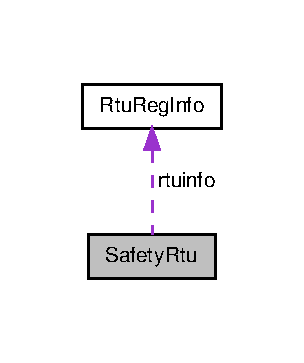
\includegraphics[width=146pt]{structSafetyRtu__coll__graph}
\end{center}
\end{figure}
\subsection*{Data Fields}
\begin{DoxyCompactItemize}
\item 
\hyperlink{structRtuRegInfo}{Rtu\-Reg\-Info} \hyperlink{structSafetyRtu_a961d9d1c9a8c9082f6cd8bcc8b3292a4}{rtuinfo}
\begin{DoxyCompactList}\small\item\em 设备头信息 \end{DoxyCompactList}\item 
\hyperlink{base_8h_ae9f2e1f80fbd243687a04febbf590e13}{Uint16} \hyperlink{structSafetyRtu_aa857a3b46e71c67a4d9c7bb83e34ffc0}{rtuplace}
\begin{DoxyCompactList}\small\item\em 设备布防状态 0x00:撤防,0x01布防,0xff表示未知 \end{DoxyCompactList}\item 
\hyperlink{base_8h_ae9f2e1f80fbd243687a04febbf590e13}{Uint16} \hyperlink{structSafetyRtu_a43fd8e2a562fea9a6ea5a7fe57fec7af}{rtuactstate}
\begin{DoxyCompactList}\small\item\em 设备动作状态 0x00:门磁合上、红外探测无入侵、门铃无意义,0x01:门磁分开、红外探测有入侵、门铃无意义; \end{DoxyCompactList}\end{DoxyCompactItemize}


\subsection{Detailed Description}
安防设备结构体 

\subsection{Field Documentation}
\hypertarget{structSafetyRtu_a43fd8e2a562fea9a6ea5a7fe57fec7af}{\index{Safety\-Rtu@{Safety\-Rtu}!rtuactstate@{rtuactstate}}
\index{rtuactstate@{rtuactstate}!SafetyRtu@{Safety\-Rtu}}
\subsubsection[{rtuactstate}]{\setlength{\rightskip}{0pt plus 5cm}{\bf Uint16} Safety\-Rtu\-::rtuactstate}}\label{structSafetyRtu_a43fd8e2a562fea9a6ea5a7fe57fec7af}


设备动作状态 0x00:门磁合上、红外探测无入侵、门铃无意义,0x01:门磁分开、红外探测有入侵、门铃无意义; 



Referenced by update\-\_\-db\-\_\-safetyrtu().

\hypertarget{structSafetyRtu_a961d9d1c9a8c9082f6cd8bcc8b3292a4}{\index{Safety\-Rtu@{Safety\-Rtu}!rtuinfo@{rtuinfo}}
\index{rtuinfo@{rtuinfo}!SafetyRtu@{Safety\-Rtu}}
\subsubsection[{rtuinfo}]{\setlength{\rightskip}{0pt plus 5cm}{\bf Rtu\-Reg\-Info} Safety\-Rtu\-::rtuinfo}}\label{structSafetyRtu_a961d9d1c9a8c9082f6cd8bcc8b3292a4}


设备头信息 



Referenced by update\-\_\-db\-\_\-safetyrtu().

\hypertarget{structSafetyRtu_aa857a3b46e71c67a4d9c7bb83e34ffc0}{\index{Safety\-Rtu@{Safety\-Rtu}!rtuplace@{rtuplace}}
\index{rtuplace@{rtuplace}!SafetyRtu@{Safety\-Rtu}}
\subsubsection[{rtuplace}]{\setlength{\rightskip}{0pt plus 5cm}{\bf Uint16} Safety\-Rtu\-::rtuplace}}\label{structSafetyRtu_aa857a3b46e71c67a4d9c7bb83e34ffc0}


设备布防状态 0x00:撤防,0x01布防,0xff表示未知 



Referenced by update\-\_\-db\-\_\-safetyrtu().



The documentation for this struct was generated from the following file\-:\begin{DoxyCompactItemize}
\item 
\hyperlink{dbbase_8h}{dbbase.\-h}\end{DoxyCompactItemize}

\hypertarget{structSceneBind}{\section{Scene\-Bind Struct Reference}
\label{structSceneBind}\index{Scene\-Bind@{Scene\-Bind}}
}


{\ttfamily \#include $<$dbbase.\-h$>$}

\subsection*{Data Fields}
\begin{DoxyCompactItemize}
\item 
\hyperlink{base_8h_ae9f2e1f80fbd243687a04febbf590e13}{Uint16} \hyperlink{structSceneBind_a92e50caa085d61d80804f44eef26c240}{id}
\begin{DoxyCompactList}\small\item\em 按键码 \end{DoxyCompactList}\item 
\hyperlink{base_8h_ae9f2e1f80fbd243687a04febbf590e13}{Uint16} \hyperlink{structSceneBind_a3d49ad98d2ccb1be6cf4f55be61b0390}{type}
\begin{DoxyCompactList}\small\item\em 绑定类型 \end{DoxyCompactList}\item 
\hyperlink{base_8h_a60cf7b3c038ce37a50796e8eaddf0b5f}{Uint32} \hyperlink{structSceneBind_aa2d7e582a6ef1f73b685bd86a3a83ab2}{add}
\begin{DoxyCompactList}\small\item\em 绑定设备/ 情景地址 \end{DoxyCompactList}\item 
\hyperlink{base_8h_a60cf7b3c038ce37a50796e8eaddf0b5f}{Uint32} \hyperlink{structSceneBind_abf48651d36a041e163a0c1ecac190288}{oper}
\begin{DoxyCompactList}\small\item\em 绑定设备继电器1-\/4的操作 \end{DoxyCompactList}\end{DoxyCompactItemize}


\subsection{Detailed Description}
情景面板尾部 部分 

\subsection{Field Documentation}
\hypertarget{structSceneBind_aa2d7e582a6ef1f73b685bd86a3a83ab2}{\index{Scene\-Bind@{Scene\-Bind}!add@{add}}
\index{add@{add}!SceneBind@{Scene\-Bind}}
\subsubsection[{add}]{\setlength{\rightskip}{0pt plus 5cm}{\bf Uint32} Scene\-Bind\-::add}}\label{structSceneBind_aa2d7e582a6ef1f73b685bd86a3a83ab2}


绑定设备/ 情景地址 



Referenced by update\-\_\-db\-\_\-scenertu().

\hypertarget{structSceneBind_a92e50caa085d61d80804f44eef26c240}{\index{Scene\-Bind@{Scene\-Bind}!id@{id}}
\index{id@{id}!SceneBind@{Scene\-Bind}}
\subsubsection[{id}]{\setlength{\rightskip}{0pt plus 5cm}{\bf Uint16} Scene\-Bind\-::id}}\label{structSceneBind_a92e50caa085d61d80804f44eef26c240}


按键码 



Referenced by update\-\_\-db\-\_\-scenertu().

\hypertarget{structSceneBind_abf48651d36a041e163a0c1ecac190288}{\index{Scene\-Bind@{Scene\-Bind}!oper@{oper}}
\index{oper@{oper}!SceneBind@{Scene\-Bind}}
\subsubsection[{oper}]{\setlength{\rightskip}{0pt plus 5cm}{\bf Uint32} Scene\-Bind\-::oper}}\label{structSceneBind_abf48651d36a041e163a0c1ecac190288}


绑定设备继电器1-\/4的操作 



Referenced by update\-\_\-db\-\_\-scenertu().

\hypertarget{structSceneBind_a3d49ad98d2ccb1be6cf4f55be61b0390}{\index{Scene\-Bind@{Scene\-Bind}!type@{type}}
\index{type@{type}!SceneBind@{Scene\-Bind}}
\subsubsection[{type}]{\setlength{\rightskip}{0pt plus 5cm}{\bf Uint16} Scene\-Bind\-::type}}\label{structSceneBind_a3d49ad98d2ccb1be6cf4f55be61b0390}


绑定类型 



Referenced by update\-\_\-db\-\_\-scenertu().



The documentation for this struct was generated from the following file\-:\begin{DoxyCompactItemize}
\item 
\hyperlink{dbbase_8h}{dbbase.\-h}\end{DoxyCompactItemize}

\hypertarget{structSceneInfo}{\section{Scene\-Info Struct Reference}
\label{structSceneInfo}\index{Scene\-Info@{Scene\-Info}}
}


{\ttfamily \#include $<$dbbase.\-h$>$}



Collaboration diagram for Scene\-Info\-:\nopagebreak
\begin{figure}[H]
\begin{center}
\leavevmode
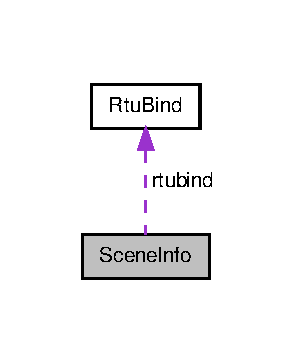
\includegraphics[width=143pt]{structSceneInfo__coll__graph}
\end{center}
\end{figure}
\subsection*{Data Fields}
\begin{DoxyCompactItemize}
\item 
\hyperlink{base_8h_a60cf7b3c038ce37a50796e8eaddf0b5f}{Uint32} \hyperlink{structSceneInfo_a71c350f2eecece851424fb6d41f3d0e1}{hostadd}
\begin{DoxyCompactList}\small\item\em 主机地址 \end{DoxyCompactList}\item 
\hyperlink{base_8h_a60cf7b3c038ce37a50796e8eaddf0b5f}{Uint32} \hyperlink{structSceneInfo_a647950844b5a2503b7c79171273eddbc}{sceneid}
\begin{DoxyCompactList}\small\item\em 情景\-I\-D \end{DoxyCompactList}\item 
\hyperlink{base_8h_a60cf7b3c038ce37a50796e8eaddf0b5f}{Uint32} \hyperlink{structSceneInfo_affa07c03b993f4fee2824da9bf11da25}{scenepicid}
\begin{DoxyCompactList}\small\item\em 情景图标\-I\-D \end{DoxyCompactList}\item 
char \hyperlink{structSceneInfo_a802bb02389ef76cdb6c30676eb65148b}{scenename} \mbox{[}32\mbox{]}
\begin{DoxyCompactList}\small\item\em 情景名字 \end{DoxyCompactList}\item 
char \hyperlink{structSceneInfo_ac27ed61e7e699160d08904fb2abfdb95}{rturegtime} \mbox{[}30\mbox{]}
\begin{DoxyCompactList}\small\item\em 注册时间 \end{DoxyCompactList}\item 
short \hyperlink{structSceneInfo_afebc902163663be26075199ba2c97d5d}{scenertunum}
\begin{DoxyCompactList}\small\item\em 情景设定的设备数 \end{DoxyCompactList}\item 
\hyperlink{structRtuBind}{Rtu\-Bind} $\ast$ \hyperlink{structSceneInfo_a04797a4b852763ec79262575bb8d3f67}{rtubind}
\begin{DoxyCompactList}\small\item\em 绑定的操作信息 \end{DoxyCompactList}\end{DoxyCompactItemize}


\subsection{Detailed Description}
创建修改情景 

\subsection{Field Documentation}
\hypertarget{structSceneInfo_a71c350f2eecece851424fb6d41f3d0e1}{\index{Scene\-Info@{Scene\-Info}!hostadd@{hostadd}}
\index{hostadd@{hostadd}!SceneInfo@{Scene\-Info}}
\subsubsection[{hostadd}]{\setlength{\rightskip}{0pt plus 5cm}{\bf Uint32} Scene\-Info\-::hostadd}}\label{structSceneInfo_a71c350f2eecece851424fb6d41f3d0e1}


主机地址 



Referenced by insert\-\_\-db\-\_\-sceneinfo(), and main().

\hypertarget{structSceneInfo_a04797a4b852763ec79262575bb8d3f67}{\index{Scene\-Info@{Scene\-Info}!rtubind@{rtubind}}
\index{rtubind@{rtubind}!SceneInfo@{Scene\-Info}}
\subsubsection[{rtubind}]{\setlength{\rightskip}{0pt plus 5cm}{\bf Rtu\-Bind}$\ast$ Scene\-Info\-::rtubind}}\label{structSceneInfo_a04797a4b852763ec79262575bb8d3f67}


绑定的操作信息 



Referenced by insert\-\_\-db\-\_\-sceneinfo(), and main().

\hypertarget{structSceneInfo_ac27ed61e7e699160d08904fb2abfdb95}{\index{Scene\-Info@{Scene\-Info}!rturegtime@{rturegtime}}
\index{rturegtime@{rturegtime}!SceneInfo@{Scene\-Info}}
\subsubsection[{rturegtime}]{\setlength{\rightskip}{0pt plus 5cm}char Scene\-Info\-::rturegtime\mbox{[}30\mbox{]}}}\label{structSceneInfo_ac27ed61e7e699160d08904fb2abfdb95}


注册时间 



Referenced by insert\-\_\-db\-\_\-sceneinfo(), and main().

\hypertarget{structSceneInfo_a647950844b5a2503b7c79171273eddbc}{\index{Scene\-Info@{Scene\-Info}!sceneid@{sceneid}}
\index{sceneid@{sceneid}!SceneInfo@{Scene\-Info}}
\subsubsection[{sceneid}]{\setlength{\rightskip}{0pt plus 5cm}{\bf Uint32} Scene\-Info\-::sceneid}}\label{structSceneInfo_a647950844b5a2503b7c79171273eddbc}


情景\-I\-D 



Referenced by insert\-\_\-db\-\_\-sceneinfo(), and main().

\hypertarget{structSceneInfo_a802bb02389ef76cdb6c30676eb65148b}{\index{Scene\-Info@{Scene\-Info}!scenename@{scenename}}
\index{scenename@{scenename}!SceneInfo@{Scene\-Info}}
\subsubsection[{scenename}]{\setlength{\rightskip}{0pt plus 5cm}char Scene\-Info\-::scenename\mbox{[}32\mbox{]}}}\label{structSceneInfo_a802bb02389ef76cdb6c30676eb65148b}


情景名字 



Referenced by insert\-\_\-db\-\_\-sceneinfo(), and main().

\hypertarget{structSceneInfo_affa07c03b993f4fee2824da9bf11da25}{\index{Scene\-Info@{Scene\-Info}!scenepicid@{scenepicid}}
\index{scenepicid@{scenepicid}!SceneInfo@{Scene\-Info}}
\subsubsection[{scenepicid}]{\setlength{\rightskip}{0pt plus 5cm}{\bf Uint32} Scene\-Info\-::scenepicid}}\label{structSceneInfo_affa07c03b993f4fee2824da9bf11da25}


情景图标\-I\-D 



Referenced by insert\-\_\-db\-\_\-sceneinfo(), and main().

\hypertarget{structSceneInfo_afebc902163663be26075199ba2c97d5d}{\index{Scene\-Info@{Scene\-Info}!scenertunum@{scenertunum}}
\index{scenertunum@{scenertunum}!SceneInfo@{Scene\-Info}}
\subsubsection[{scenertunum}]{\setlength{\rightskip}{0pt plus 5cm}short Scene\-Info\-::scenertunum}}\label{structSceneInfo_afebc902163663be26075199ba2c97d5d}


情景设定的设备数 



Referenced by insert\-\_\-db\-\_\-sceneinfo(), and main().



The documentation for this struct was generated from the following file\-:\begin{DoxyCompactItemize}
\item 
\hyperlink{dbbase_8h}{dbbase.\-h}\end{DoxyCompactItemize}

\hypertarget{structSceneRtu}{\section{Scene\-Rtu Struct Reference}
\label{structSceneRtu}\index{Scene\-Rtu@{Scene\-Rtu}}
}


{\ttfamily \#include $<$dbbase.\-h$>$}



Collaboration diagram for Scene\-Rtu\-:\nopagebreak
\begin{figure}[H]
\begin{center}
\leavevmode
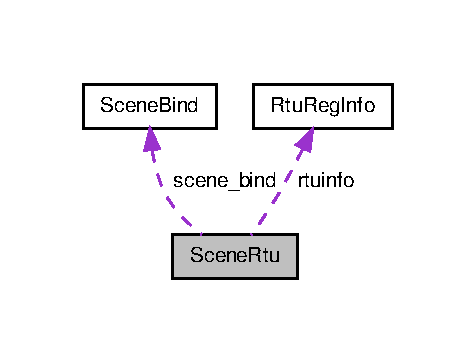
\includegraphics[width=228pt]{structSceneRtu__coll__graph}
\end{center}
\end{figure}
\subsection*{Data Fields}
\begin{DoxyCompactItemize}
\item 
\hyperlink{structRtuRegInfo}{Rtu\-Reg\-Info} \hyperlink{structSceneRtu_a8850884f48b4d42495efce8ba6cdab7b}{rtuinfo}
\begin{DoxyCompactList}\small\item\em 设备头信息 \end{DoxyCompactList}\item 
\hyperlink{base_8h_ae9f2e1f80fbd243687a04febbf590e13}{Uint16} \hyperlink{structSceneRtu_aa094ff659f108ee77a08b35bcba85bb6}{bind\-\_\-num}
\item 
\hyperlink{structSceneBind}{Scene\-Bind} \hyperlink{structSceneRtu_a308c1e20b977bbfcf203751cecac8e2f}{scene\-\_\-bind} \mbox{[}4\mbox{]}
\end{DoxyCompactItemize}


\subsection{Detailed Description}
情景面板 结构体 

\subsection{Field Documentation}
\hypertarget{structSceneRtu_aa094ff659f108ee77a08b35bcba85bb6}{\index{Scene\-Rtu@{Scene\-Rtu}!bind\-\_\-num@{bind\-\_\-num}}
\index{bind\-\_\-num@{bind\-\_\-num}!SceneRtu@{Scene\-Rtu}}
\subsubsection[{bind\-\_\-num}]{\setlength{\rightskip}{0pt plus 5cm}{\bf Uint16} Scene\-Rtu\-::bind\-\_\-num}}\label{structSceneRtu_aa094ff659f108ee77a08b35bcba85bb6}


Referenced by update\-\_\-db\-\_\-scenertu().

\hypertarget{structSceneRtu_a8850884f48b4d42495efce8ba6cdab7b}{\index{Scene\-Rtu@{Scene\-Rtu}!rtuinfo@{rtuinfo}}
\index{rtuinfo@{rtuinfo}!SceneRtu@{Scene\-Rtu}}
\subsubsection[{rtuinfo}]{\setlength{\rightskip}{0pt plus 5cm}{\bf Rtu\-Reg\-Info} Scene\-Rtu\-::rtuinfo}}\label{structSceneRtu_a8850884f48b4d42495efce8ba6cdab7b}


设备头信息 



Referenced by update\-\_\-db\-\_\-scenertu().

\hypertarget{structSceneRtu_a308c1e20b977bbfcf203751cecac8e2f}{\index{Scene\-Rtu@{Scene\-Rtu}!scene\-\_\-bind@{scene\-\_\-bind}}
\index{scene\-\_\-bind@{scene\-\_\-bind}!SceneRtu@{Scene\-Rtu}}
\subsubsection[{scene\-\_\-bind}]{\setlength{\rightskip}{0pt plus 5cm}{\bf Scene\-Bind} Scene\-Rtu\-::scene\-\_\-bind\mbox{[}4\mbox{]}}}\label{structSceneRtu_a308c1e20b977bbfcf203751cecac8e2f}


Referenced by update\-\_\-db\-\_\-scenertu().



The documentation for this struct was generated from the following file\-:\begin{DoxyCompactItemize}
\item 
\hyperlink{dbbase_8h}{dbbase.\-h}\end{DoxyCompactItemize}

\hypertarget{structTaskInfo}{\section{Task\-Info Struct Reference}
\label{structTaskInfo}\index{Task\-Info@{Task\-Info}}
}


{\ttfamily \#include $<$dbbase.\-h$>$}



Collaboration diagram for Task\-Info\-:\nopagebreak
\begin{figure}[H]
\begin{center}
\leavevmode
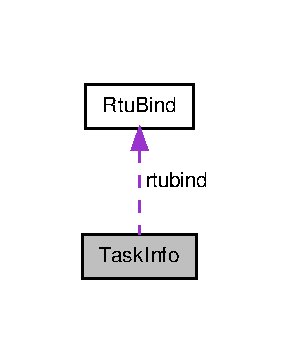
\includegraphics[width=140pt]{structTaskInfo__coll__graph}
\end{center}
\end{figure}
\subsection*{Data Fields}
\begin{DoxyCompactItemize}
\item 
\hyperlink{base_8h_a60cf7b3c038ce37a50796e8eaddf0b5f}{Uint32} \hyperlink{structTaskInfo_a633cb279d0c214d3eba9da3d26f5a020}{hostadd}
\begin{DoxyCompactList}\small\item\em 主机地址 \end{DoxyCompactList}\item 
\hyperlink{base_8h_a60cf7b3c038ce37a50796e8eaddf0b5f}{Uint32} \hyperlink{structTaskInfo_a27224eae1effa0e80bc2fa52dde59692}{taskid}
\begin{DoxyCompactList}\small\item\em 任务id \end{DoxyCompactList}\item 
char \hyperlink{structTaskInfo_a93bbd541a14b0eb3be4d81df457f53c0}{taskname} \mbox{[}32\mbox{]}
\begin{DoxyCompactList}\small\item\em 任务名称 \end{DoxyCompactList}\item 
\hyperlink{base_8h_a60cf7b3c038ce37a50796e8eaddf0b5f}{Uint32} \hyperlink{structTaskInfo_ab853cd6598db69ad460ab8ae9efa49b6}{taskpicid}
\begin{DoxyCompactList}\small\item\em 任务图标 id \end{DoxyCompactList}\item 
char \hyperlink{structTaskInfo_af4123b5a228c33d071e00474447e3a7b}{taskregtime} \mbox{[}30\mbox{]}
\begin{DoxyCompactList}\small\item\em 任务注册时间 \end{DoxyCompactList}\item 
\hyperlink{base_8h_ae9f2e1f80fbd243687a04febbf590e13}{Uint16} \hyperlink{structTaskInfo_a585a387b5d639defa31bb8511d0c3b48}{taskcycle}
\begin{DoxyCompactList}\small\item\em 任务循环 标志 \end{DoxyCompactList}\item 
\hyperlink{base_8h_ae9f2e1f80fbd243687a04febbf590e13}{Uint16} \hyperlink{structTaskInfo_a82ca17b1ed9c9059cf624032fd25a15d}{taskstdtime} \mbox{[}3\mbox{]}
\begin{DoxyCompactList}\small\item\em 任务执行时间 hour \-: min \-: sec \end{DoxyCompactList}\item 
\hyperlink{base_8h_a60cf7b3c038ce37a50796e8eaddf0b5f}{Uint32} \hyperlink{structTaskInfo_a0bfa1e0ae661b9841bd77b14b8002c2a}{taskrtunum}
\begin{DoxyCompactList}\small\item\em 绑定设备个数 \end{DoxyCompactList}\item 
\hyperlink{structRtuBind}{Rtu\-Bind} $\ast$ \hyperlink{structTaskInfo_abcd620f1a510696638104149f8c06e2c}{rtubind}
\begin{DoxyCompactList}\small\item\em 绑定的设备信息 \end{DoxyCompactList}\end{DoxyCompactItemize}


\subsection{Detailed Description}
定时任务结构体 

\subsection{Field Documentation}
\hypertarget{structTaskInfo_a633cb279d0c214d3eba9da3d26f5a020}{\index{Task\-Info@{Task\-Info}!hostadd@{hostadd}}
\index{hostadd@{hostadd}!TaskInfo@{Task\-Info}}
\subsubsection[{hostadd}]{\setlength{\rightskip}{0pt plus 5cm}{\bf Uint32} Task\-Info\-::hostadd}}\label{structTaskInfo_a633cb279d0c214d3eba9da3d26f5a020}


主机地址 



Referenced by insert\-\_\-db\-\_\-taskinfo(), and main().

\hypertarget{structTaskInfo_abcd620f1a510696638104149f8c06e2c}{\index{Task\-Info@{Task\-Info}!rtubind@{rtubind}}
\index{rtubind@{rtubind}!TaskInfo@{Task\-Info}}
\subsubsection[{rtubind}]{\setlength{\rightskip}{0pt plus 5cm}{\bf Rtu\-Bind}$\ast$ Task\-Info\-::rtubind}}\label{structTaskInfo_abcd620f1a510696638104149f8c06e2c}


绑定的设备信息 



Referenced by insert\-\_\-db\-\_\-taskinfo(), and main().

\hypertarget{structTaskInfo_a585a387b5d639defa31bb8511d0c3b48}{\index{Task\-Info@{Task\-Info}!taskcycle@{taskcycle}}
\index{taskcycle@{taskcycle}!TaskInfo@{Task\-Info}}
\subsubsection[{taskcycle}]{\setlength{\rightskip}{0pt plus 5cm}{\bf Uint16} Task\-Info\-::taskcycle}}\label{structTaskInfo_a585a387b5d639defa31bb8511d0c3b48}


任务循环 标志 



Referenced by insert\-\_\-db\-\_\-taskinfo().

\hypertarget{structTaskInfo_a27224eae1effa0e80bc2fa52dde59692}{\index{Task\-Info@{Task\-Info}!taskid@{taskid}}
\index{taskid@{taskid}!TaskInfo@{Task\-Info}}
\subsubsection[{taskid}]{\setlength{\rightskip}{0pt plus 5cm}{\bf Uint32} Task\-Info\-::taskid}}\label{structTaskInfo_a27224eae1effa0e80bc2fa52dde59692}


任务id 



Referenced by insert\-\_\-db\-\_\-taskinfo(), and main().

\hypertarget{structTaskInfo_a93bbd541a14b0eb3be4d81df457f53c0}{\index{Task\-Info@{Task\-Info}!taskname@{taskname}}
\index{taskname@{taskname}!TaskInfo@{Task\-Info}}
\subsubsection[{taskname}]{\setlength{\rightskip}{0pt plus 5cm}char Task\-Info\-::taskname\mbox{[}32\mbox{]}}}\label{structTaskInfo_a93bbd541a14b0eb3be4d81df457f53c0}


任务名称 



Referenced by insert\-\_\-db\-\_\-taskinfo(), and main().

\hypertarget{structTaskInfo_ab853cd6598db69ad460ab8ae9efa49b6}{\index{Task\-Info@{Task\-Info}!taskpicid@{taskpicid}}
\index{taskpicid@{taskpicid}!TaskInfo@{Task\-Info}}
\subsubsection[{taskpicid}]{\setlength{\rightskip}{0pt plus 5cm}{\bf Uint32} Task\-Info\-::taskpicid}}\label{structTaskInfo_ab853cd6598db69ad460ab8ae9efa49b6}


任务图标 id 



Referenced by insert\-\_\-db\-\_\-taskinfo().

\hypertarget{structTaskInfo_af4123b5a228c33d071e00474447e3a7b}{\index{Task\-Info@{Task\-Info}!taskregtime@{taskregtime}}
\index{taskregtime@{taskregtime}!TaskInfo@{Task\-Info}}
\subsubsection[{taskregtime}]{\setlength{\rightskip}{0pt plus 5cm}char Task\-Info\-::taskregtime\mbox{[}30\mbox{]}}}\label{structTaskInfo_af4123b5a228c33d071e00474447e3a7b}


任务注册时间 



Referenced by insert\-\_\-db\-\_\-taskinfo(), and main().

\hypertarget{structTaskInfo_a0bfa1e0ae661b9841bd77b14b8002c2a}{\index{Task\-Info@{Task\-Info}!taskrtunum@{taskrtunum}}
\index{taskrtunum@{taskrtunum}!TaskInfo@{Task\-Info}}
\subsubsection[{taskrtunum}]{\setlength{\rightskip}{0pt plus 5cm}{\bf Uint32} Task\-Info\-::taskrtunum}}\label{structTaskInfo_a0bfa1e0ae661b9841bd77b14b8002c2a}


绑定设备个数 



Referenced by insert\-\_\-db\-\_\-taskinfo(), and main().

\hypertarget{structTaskInfo_a82ca17b1ed9c9059cf624032fd25a15d}{\index{Task\-Info@{Task\-Info}!taskstdtime@{taskstdtime}}
\index{taskstdtime@{taskstdtime}!TaskInfo@{Task\-Info}}
\subsubsection[{taskstdtime}]{\setlength{\rightskip}{0pt plus 5cm}{\bf Uint16} Task\-Info\-::taskstdtime\mbox{[}3\mbox{]}}}\label{structTaskInfo_a82ca17b1ed9c9059cf624032fd25a15d}


任务执行时间 hour \-: min \-: sec 



Referenced by insert\-\_\-db\-\_\-taskinfo().



The documentation for this struct was generated from the following file\-:\begin{DoxyCompactItemize}
\item 
\hyperlink{dbbase_8h}{dbbase.\-h}\end{DoxyCompactItemize}

\chapter{File Documentation}
\hypertarget{base_8h}{\section{base.\-h File Reference}
\label{base_8h}\index{base.\-h@{base.\-h}}
}


常见类型,调试开关定义 @  


{\ttfamily \#include $<$stdio.\-h$>$}\\*
{\ttfamily \#include $<$stdlib.\-h$>$}\\*
Include dependency graph for base.\-h\-:\nopagebreak
\begin{figure}[H]
\begin{center}
\leavevmode
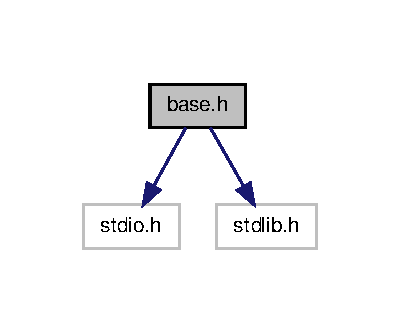
\includegraphics[width=192pt]{base_8h__incl}
\end{center}
\end{figure}
This graph shows which files directly or indirectly include this file\-:\nopagebreak
\begin{figure}[H]
\begin{center}
\leavevmode
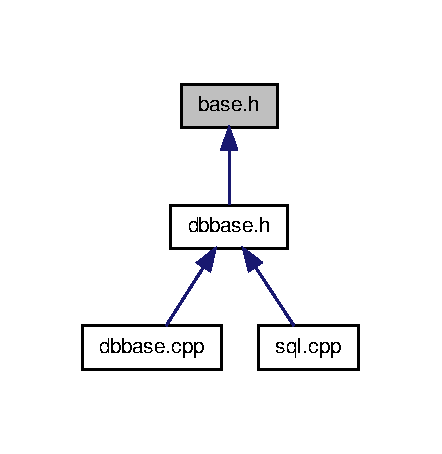
\includegraphics[width=212pt]{base_8h__dep__incl}
\end{center}
\end{figure}
\subsection*{Macros}
\begin{DoxyCompactItemize}
\item 
\#define \hyperlink{base_8h_ac8bab6bccfa5a1766f88032f6b8485f1}{L\-O\-G\-\_\-\-E\-R\-R\-O\-R}(format, args...)
\item 
\#define \hyperlink{base_8h_aa7558f9398d2befa813c73e131e8bdcf}{L\-O\-G\-\_\-\-P\-R\-I\-N\-T}(format, args...)
\item 
\#define \hyperlink{base_8h_a432138093c53d7580af9ec5c5dca387f}{E\-N\-A\-B\-L\-E\-\_\-\-D\-E\-B\-U\-G}
\item 
\#define \hyperlink{base_8h_a1f953b078595aed0c003eda86c62bde2}{L\-O\-G\-\_\-\-D\-E\-B\-U\-G}(format, args...)
\end{DoxyCompactItemize}
\subsection*{Typedefs}
\begin{DoxyCompactItemize}
\item 
typedef char \hyperlink{base_8h_a3832cc814f0e7129add9a1cf7201c7ca}{Int8}
\item 
typedef signed short \hyperlink{base_8h_a5708a0dfbf256454e50a033ce7cceb8b}{Int16}
\item 
typedef int \hyperlink{base_8h_adf1ef98b7070177c7c709b0b82276a07}{Int32}
\item 
typedef long \hyperlink{base_8h_a087291516e13bb56547918e3832026b5}{Int64}
\item 
typedef unsigned char \hyperlink{base_8h_af84840501dec18061d18a68c162a8fa2}{Uint8}
\item 
typedef unsigned short \hyperlink{base_8h_ae9f2e1f80fbd243687a04febbf590e13}{Uint16}
\item 
typedef unsigned int \hyperlink{base_8h_a60cf7b3c038ce37a50796e8eaddf0b5f}{Uint32}
\item 
typedef unsigned long \hyperlink{base_8h_a687eb0325075867ce19e6e27eeac4e2e}{Uint64}
\item 
typedef float \hyperlink{base_8h_a87d38f886e617ced2698fc55afa07637}{Float32}
\item 
typedef double \hyperlink{base_8h_a3f1431cb9f76da10f59246d1d743dc2c}{Float64}
\end{DoxyCompactItemize}
\subsection*{Functions}
\begin{DoxyCompactItemize}
\item 
static unsigned \hyperlink{base_8h_a651442fd84e46cd7637e76ccf59a3f4e}{get\-\_\-current\-\_\-time} (void)
\item 
static void \hyperlink{base_8h_ab8a6e9d8a4bea9ec5f6583cd2a8af735}{get\-\_\-sys\-\_\-time} (char $\ast$strtime)
\item 
static void \hyperlink{base_8h_a47e5e257a7e7173ffda21017ecd22367}{start\-\_\-time} ()
\end{DoxyCompactItemize}


\subsection{Detailed Description}
常见类型,调试开关定义 @ 

\subsection{Macro Definition Documentation}
\hypertarget{base_8h_a432138093c53d7580af9ec5c5dca387f}{\index{base.\-h@{base.\-h}!E\-N\-A\-B\-L\-E\-\_\-\-D\-E\-B\-U\-G@{E\-N\-A\-B\-L\-E\-\_\-\-D\-E\-B\-U\-G}}
\index{E\-N\-A\-B\-L\-E\-\_\-\-D\-E\-B\-U\-G@{E\-N\-A\-B\-L\-E\-\_\-\-D\-E\-B\-U\-G}!base.h@{base.\-h}}
\subsubsection[{E\-N\-A\-B\-L\-E\-\_\-\-D\-E\-B\-U\-G}]{\setlength{\rightskip}{0pt plus 5cm}\#define E\-N\-A\-B\-L\-E\-\_\-\-D\-E\-B\-U\-G}}\label{base_8h_a432138093c53d7580af9ec5c5dca387f}
调试开关 \hypertarget{base_8h_a1f953b078595aed0c003eda86c62bde2}{\index{base.\-h@{base.\-h}!L\-O\-G\-\_\-\-D\-E\-B\-U\-G@{L\-O\-G\-\_\-\-D\-E\-B\-U\-G}}
\index{L\-O\-G\-\_\-\-D\-E\-B\-U\-G@{L\-O\-G\-\_\-\-D\-E\-B\-U\-G}!base.h@{base.\-h}}
\subsubsection[{L\-O\-G\-\_\-\-D\-E\-B\-U\-G}]{\setlength{\rightskip}{0pt plus 5cm}\#define L\-O\-G\-\_\-\-D\-E\-B\-U\-G(
\begin{DoxyParamCaption}
\item[{}]{format, }
\item[{}]{args...}
\end{DoxyParamCaption}
)}}\label{base_8h_a1f953b078595aed0c003eda86c62bde2}
{\bfseries Value\-:}
\begin{DoxyCode}
\textcolor{keywordflow}{do} \{ \(\backslash\)
    fprintf(stdout, \textcolor{stringliteral}{"Debug: "}format, ##args);   \(\backslash\)
    fflush(stdout);   \(\backslash\)
\} \textcolor{keywordflow}{while} (0)
\end{DoxyCode}
调试输出 

Referenced by db\-\_\-insert\-\_\-query(), db\-\_\-select\-\_\-query(), db\-\_\-update\-\_\-query(), delete\-\_\-db\-\_\-host(), delete\-\_\-db\-\_\-rtu(), Dupicate\-Key\-Update\-Query(), Get\-Host\-Count(), Get\-Host\-Id\-By\-Name(), Get\-Ip\-By\-Host\-Add(), select\-\_\-db\-\_\-hostinfo(), select\-\_\-query(), start\-\_\-time(), and update\-\_\-db\-\_\-nativertu().

\hypertarget{base_8h_ac8bab6bccfa5a1766f88032f6b8485f1}{\index{base.\-h@{base.\-h}!L\-O\-G\-\_\-\-E\-R\-R\-O\-R@{L\-O\-G\-\_\-\-E\-R\-R\-O\-R}}
\index{L\-O\-G\-\_\-\-E\-R\-R\-O\-R@{L\-O\-G\-\_\-\-E\-R\-R\-O\-R}!base.h@{base.\-h}}
\subsubsection[{L\-O\-G\-\_\-\-E\-R\-R\-O\-R}]{\setlength{\rightskip}{0pt plus 5cm}\#define L\-O\-G\-\_\-\-E\-R\-R\-O\-R(
\begin{DoxyParamCaption}
\item[{}]{format, }
\item[{}]{args...}
\end{DoxyParamCaption}
)}}\label{base_8h_ac8bab6bccfa5a1766f88032f6b8485f1}
{\bfseries Value\-:}
\begin{DoxyCode}
\textcolor{keywordflow}{do} \{ \(\backslash\)
    fprintf(stdout, \textcolor{stringliteral}{"ERROR %s, %d, "}format, \_\_FILE\_\_, \_\_LINE\_\_, ##args);   \(\backslash\)
    fflush(stdout);   \(\backslash\)
\} \textcolor{keywordflow}{while} (0)
\end{DoxyCode}
错误输出 

Referenced by db\-\_\-insert\-\_\-query(), db\-\_\-select\-\_\-query(), delete\-\_\-db\-\_\-host(), delete\-\_\-db\-\_\-rtu(), find\-Hostname(), find\-Rtuadd(), Get\-Host\-Count(), Get\-Host\-Id\-By\-Name(), Get\-Ip\-By\-Host\-Add(), insert\-\_\-db\-\_\-apprtu(), insert\-\_\-db\-\_\-host(), insert\-\_\-db\-\_\-rtu(), insert\-\_\-db\-\_\-sceneinfo(), insert\-\_\-db\-\_\-taskinfo(), insert\-\_\-mysql(), select\-\_\-db\-\_\-hostinfo(), select\-\_\-query(), update\-\_\-db\-\_\-detectorrtu(), update\-\_\-db\-\_\-host(), update\-\_\-db\-\_\-nativertu(), and update\-\_\-db\-\_\-safetypwd().

\hypertarget{base_8h_aa7558f9398d2befa813c73e131e8bdcf}{\index{base.\-h@{base.\-h}!L\-O\-G\-\_\-\-P\-R\-I\-N\-T@{L\-O\-G\-\_\-\-P\-R\-I\-N\-T}}
\index{L\-O\-G\-\_\-\-P\-R\-I\-N\-T@{L\-O\-G\-\_\-\-P\-R\-I\-N\-T}!base.h@{base.\-h}}
\subsubsection[{L\-O\-G\-\_\-\-P\-R\-I\-N\-T}]{\setlength{\rightskip}{0pt plus 5cm}\#define L\-O\-G\-\_\-\-P\-R\-I\-N\-T(
\begin{DoxyParamCaption}
\item[{}]{format, }
\item[{}]{args...}
\end{DoxyParamCaption}
)}}\label{base_8h_aa7558f9398d2befa813c73e131e8bdcf}
{\bfseries Value\-:}
\begin{DoxyCode}
\textcolor{keywordflow}{do} \{ \(\backslash\)
    fprintf(stdout, \textcolor{stringliteral}{"Info: "}format, ##args);   \(\backslash\)
    fflush(stdout);   \(\backslash\)
\} \textcolor{keywordflow}{while} (0)
\end{DoxyCode}
打印输出 

Referenced by insert\-\_\-db\-\_\-host(), and start\-\_\-time().



\subsection{Typedef Documentation}
\hypertarget{base_8h_a87d38f886e617ced2698fc55afa07637}{\index{base.\-h@{base.\-h}!Float32@{Float32}}
\index{Float32@{Float32}!base.h@{base.\-h}}
\subsubsection[{Float32}]{\setlength{\rightskip}{0pt plus 5cm}typedef float {\bf Float32}}}\label{base_8h_a87d38f886e617ced2698fc55afa07637}
\hypertarget{base_8h_a3f1431cb9f76da10f59246d1d743dc2c}{\index{base.\-h@{base.\-h}!Float64@{Float64}}
\index{Float64@{Float64}!base.h@{base.\-h}}
\subsubsection[{Float64}]{\setlength{\rightskip}{0pt plus 5cm}typedef double {\bf Float64}}}\label{base_8h_a3f1431cb9f76da10f59246d1d743dc2c}
\hypertarget{base_8h_a5708a0dfbf256454e50a033ce7cceb8b}{\index{base.\-h@{base.\-h}!Int16@{Int16}}
\index{Int16@{Int16}!base.h@{base.\-h}}
\subsubsection[{Int16}]{\setlength{\rightskip}{0pt plus 5cm}typedef signed short {\bf Int16}}}\label{base_8h_a5708a0dfbf256454e50a033ce7cceb8b}
S\-I\-G\-N\-E\-D 16-\/bit data type \hypertarget{base_8h_adf1ef98b7070177c7c709b0b82276a07}{\index{base.\-h@{base.\-h}!Int32@{Int32}}
\index{Int32@{Int32}!base.h@{base.\-h}}
\subsubsection[{Int32}]{\setlength{\rightskip}{0pt plus 5cm}typedef int {\bf Int32}}}\label{base_8h_adf1ef98b7070177c7c709b0b82276a07}
S\-I\-G\-N\-E\-D 32-\/bit data type \hypertarget{base_8h_a087291516e13bb56547918e3832026b5}{\index{base.\-h@{base.\-h}!Int64@{Int64}}
\index{Int64@{Int64}!base.h@{base.\-h}}
\subsubsection[{Int64}]{\setlength{\rightskip}{0pt plus 5cm}typedef long {\bf Int64}}}\label{base_8h_a087291516e13bb56547918e3832026b5}
S\-I\-G\-N\-E\-D 64-\/bit data type \hypertarget{base_8h_a3832cc814f0e7129add9a1cf7201c7ca}{\index{base.\-h@{base.\-h}!Int8@{Int8}}
\index{Int8@{Int8}!base.h@{base.\-h}}
\subsubsection[{Int8}]{\setlength{\rightskip}{0pt plus 5cm}typedef char {\bf Int8}}}\label{base_8h_a3832cc814f0e7129add9a1cf7201c7ca}
S\-I\-G\-N\-E\-D 8-\/bit data type \hypertarget{base_8h_ae9f2e1f80fbd243687a04febbf590e13}{\index{base.\-h@{base.\-h}!Uint16@{Uint16}}
\index{Uint16@{Uint16}!base.h@{base.\-h}}
\subsubsection[{Uint16}]{\setlength{\rightskip}{0pt plus 5cm}typedef unsigned short {\bf Uint16}}}\label{base_8h_ae9f2e1f80fbd243687a04febbf590e13}
U\-N\-S\-I\-G\-N\-E\-D 16-\/bit data type \hypertarget{base_8h_a60cf7b3c038ce37a50796e8eaddf0b5f}{\index{base.\-h@{base.\-h}!Uint32@{Uint32}}
\index{Uint32@{Uint32}!base.h@{base.\-h}}
\subsubsection[{Uint32}]{\setlength{\rightskip}{0pt plus 5cm}typedef unsigned int {\bf Uint32}}}\label{base_8h_a60cf7b3c038ce37a50796e8eaddf0b5f}
U\-N\-S\-I\-G\-N\-E\-D 32-\/bit data type \hypertarget{base_8h_a687eb0325075867ce19e6e27eeac4e2e}{\index{base.\-h@{base.\-h}!Uint64@{Uint64}}
\index{Uint64@{Uint64}!base.h@{base.\-h}}
\subsubsection[{Uint64}]{\setlength{\rightskip}{0pt plus 5cm}typedef unsigned long {\bf Uint64}}}\label{base_8h_a687eb0325075867ce19e6e27eeac4e2e}
U\-N\-S\-I\-G\-N\-E\-D 64-\/bit data type \hypertarget{base_8h_af84840501dec18061d18a68c162a8fa2}{\index{base.\-h@{base.\-h}!Uint8@{Uint8}}
\index{Uint8@{Uint8}!base.h@{base.\-h}}
\subsubsection[{Uint8}]{\setlength{\rightskip}{0pt plus 5cm}typedef unsigned char {\bf Uint8}}}\label{base_8h_af84840501dec18061d18a68c162a8fa2}
U\-N\-S\-I\-G\-N\-E\-D 8-\/bit data type 

\subsection{Function Documentation}
\hypertarget{base_8h_a651442fd84e46cd7637e76ccf59a3f4e}{\index{base.\-h@{base.\-h}!get\-\_\-current\-\_\-time@{get\-\_\-current\-\_\-time}}
\index{get\-\_\-current\-\_\-time@{get\-\_\-current\-\_\-time}!base.h@{base.\-h}}
\subsubsection[{get\-\_\-current\-\_\-time}]{\setlength{\rightskip}{0pt plus 5cm}static unsigned get\-\_\-current\-\_\-time (
\begin{DoxyParamCaption}
\item[{void}]{}
\end{DoxyParamCaption}
)\hspace{0.3cm}{\ttfamily [inline]}, {\ttfamily [static]}}}\label{base_8h_a651442fd84e46cd7637e76ccf59a3f4e}
得到当前时间 以s为单位 

Referenced by start\-\_\-time().



Here is the caller graph for this function\-:\nopagebreak
\begin{figure}[H]
\begin{center}
\leavevmode
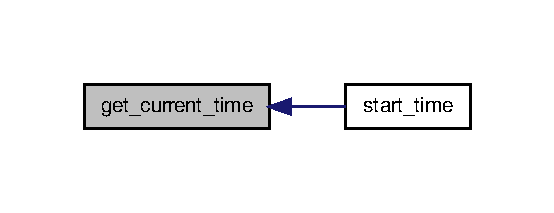
\includegraphics[width=266pt]{base_8h_a651442fd84e46cd7637e76ccf59a3f4e_icgraph}
\end{center}
\end{figure}


\hypertarget{base_8h_ab8a6e9d8a4bea9ec5f6583cd2a8af735}{\index{base.\-h@{base.\-h}!get\-\_\-sys\-\_\-time@{get\-\_\-sys\-\_\-time}}
\index{get\-\_\-sys\-\_\-time@{get\-\_\-sys\-\_\-time}!base.h@{base.\-h}}
\subsubsection[{get\-\_\-sys\-\_\-time}]{\setlength{\rightskip}{0pt plus 5cm}static void get\-\_\-sys\-\_\-time (
\begin{DoxyParamCaption}
\item[{char $\ast$}]{strtime}
\end{DoxyParamCaption}
)\hspace{0.3cm}{\ttfamily [static]}}}\label{base_8h_ab8a6e9d8a4bea9ec5f6583cd2a8af735}
得到系统时间 

Referenced by main(), and update\-\_\-db\-\_\-host().



Here is the caller graph for this function\-:\nopagebreak
\begin{figure}[H]
\begin{center}
\leavevmode
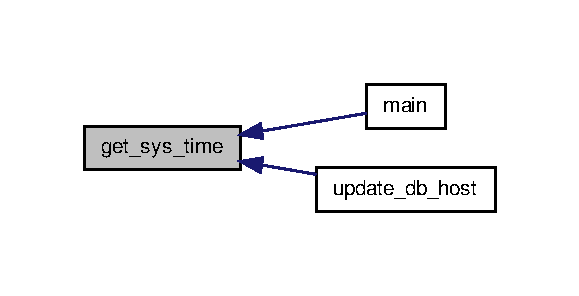
\includegraphics[width=278pt]{base_8h_ab8a6e9d8a4bea9ec5f6583cd2a8af735_icgraph}
\end{center}
\end{figure}


\hypertarget{base_8h_a47e5e257a7e7173ffda21017ecd22367}{\index{base.\-h@{base.\-h}!start\-\_\-time@{start\-\_\-time}}
\index{start\-\_\-time@{start\-\_\-time}!base.h@{base.\-h}}
\subsubsection[{start\-\_\-time}]{\setlength{\rightskip}{0pt plus 5cm}static void start\-\_\-time (
\begin{DoxyParamCaption}
{}
\end{DoxyParamCaption}
)\hspace{0.3cm}{\ttfamily [static]}}}\label{base_8h_a47e5e257a7e7173ffda21017ecd22367}
打印当前时间 

References get\-\_\-current\-\_\-time(), L\-O\-G\-\_\-\-D\-E\-B\-U\-G, and L\-O\-G\-\_\-\-P\-R\-I\-N\-T.



Here is the call graph for this function\-:\nopagebreak
\begin{figure}[H]
\begin{center}
\leavevmode
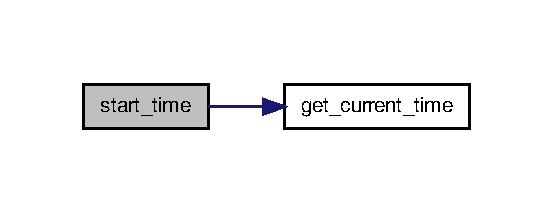
\includegraphics[width=266pt]{base_8h_a47e5e257a7e7173ffda21017ecd22367_cgraph}
\end{center}
\end{figure}



\hypertarget{dbbase_8cpp}{\section{dbbase.\-cpp File Reference}
\label{dbbase_8cpp}\index{dbbase.\-cpp@{dbbase.\-cpp}}
}


数据库接口实现  


{\ttfamily \#include \char`\"{}dbbase.\-h\char`\"{}}\\*
Include dependency graph for dbbase.\-cpp\-:\nopagebreak
\begin{figure}[H]
\begin{center}
\leavevmode
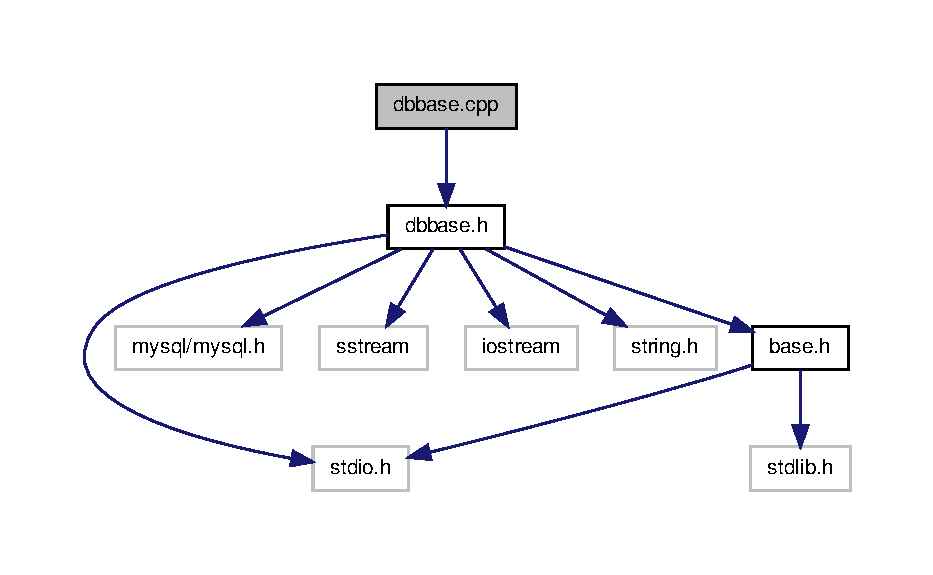
\includegraphics[width=350pt]{dbbase_8cpp__incl}
\end{center}
\end{figure}
\subsection*{Functions}
\begin{DoxyCompactItemize}
\item 
bool \hyperlink{dbbase_8cpp_a55f5cb081a0fc3774070718f283746d6}{Is\-Native\-Rtu} (\hyperlink{base_8h_af84840501dec18061d18a68c162a8fa2}{Uint8} type)
\begin{DoxyCompactList}\small\item\em Is\-Native\-Rtu 查看某设备是否是常规设备 \end{DoxyCompactList}\item 
bool \hyperlink{dbbase_8cpp_ae130c9ff11734f9b283c749b1c682659}{Is\-Safety\-Rtu} (\hyperlink{base_8h_af84840501dec18061d18a68c162a8fa2}{Uint8} type)
\begin{DoxyCompactList}\small\item\em Is\-Safety\-Rtu 查看某设备是否是安防设备 \end{DoxyCompactList}\item 
int \hyperlink{dbbase_8cpp_affefb171c935f2ae5832d0ca8091798f}{init\-\_\-mysql} (\hyperlink{structMysqlConInfo}{Mysql\-Con\-Info} $\ast$info)
\begin{DoxyCompactList}\small\item\em init\-\_\-mysql 初始化mysql , 连接,指定数据库 \end{DoxyCompactList}\item 
std\-::string \hyperlink{dbbase_8cpp_af89ddd8c208010e4477750f84849f9bf}{get\-\_\-table\-\_\-name} (\hyperlink{base_8h_af84840501dec18061d18a68c162a8fa2}{Uint8} type)
\begin{DoxyCompactList}\small\item\em get\-\_\-table\-\_\-name 根据设备类型 拿到对应的表名 \end{DoxyCompactList}\item 
static int \hyperlink{dbbase_8cpp_a45f3ac6076b939b77778a8d8a2aebde6}{check\-\_\-connect} ()
\begin{DoxyCompactList}\small\item\em check\-\_\-connect 检查连接 \end{DoxyCompactList}\item 
static int \hyperlink{dbbase_8cpp_afe0ea3530d4cbbbf870292d37df7ac9e}{insert\-\_\-mysql} (string sql\-\_\-cmd)
\begin{DoxyCompactList}\small\item\em insert\-\_\-mysql 数据库基本插入操作 \end{DoxyCompactList}\item 
static int \hyperlink{dbbase_8cpp_ae3ea82d0883ed39d63abe2f2e5cde42f}{db\-\_\-insert\-\_\-query} (const string \&colstr, const string \&valstr, const string \&tablename)
\begin{DoxyCompactList}\small\item\em db\-\_\-insert\-\_\-query 数据库插入 \end{DoxyCompactList}\item 
static int \hyperlink{dbbase_8cpp_ac9d1db67754ebd6ac53cd4ce185a22cd}{Dupicate\-Key\-Update\-Query} (const string \&colstr, const string \&valstr, const string \&updatestr, const string \&tablename)
\begin{DoxyCompactList}\small\item\em Dupicate\-Key\-Update\-Query 更新、插入查询:存在则更新不存在则插入 \end{DoxyCompactList}\item 
static int \hyperlink{dbbase_8cpp_acdefe48f4a7a750062898c54c5ecd356}{select\-\_\-query} (const string \&sql, string \&retstr)
\begin{DoxyCompactList}\small\item\em select\-\_\-query 查找操作 \end{DoxyCompactList}\item 
static \hyperlink{base_8h_a60cf7b3c038ce37a50796e8eaddf0b5f}{Uint32} \hyperlink{dbbase_8cpp_a7f355040a91d1275a6ac9a9490025717}{db\-\_\-select\-\_\-query} (const string \&colstr, const string \&wheresrt, const string \&tablename, string \&retstr)
\begin{DoxyCompactList}\small\item\em db\-\_\-select\-\_\-query 查找操作 \end{DoxyCompactList}\item 
static int \hyperlink{dbbase_8cpp_a09e73ba1c0460f0f548fffa8f8aa8ebb}{db\-\_\-update\-\_\-query} (const string \&setstr, const string \&wherestr, const string \&tablename)
\begin{DoxyCompactList}\small\item\em db\-\_\-update\-\_\-query 更新查询 \end{DoxyCompactList}\item 
static int \hyperlink{dbbase_8cpp_aec7bbc2b50281d325bd7e99661ef5c60}{find\-Rtuadd} (\hyperlink{base_8h_a60cf7b3c038ce37a50796e8eaddf0b5f}{Uint32} rtuadd, const string \&tablename)
\item 
int \hyperlink{dbbase_8cpp_a7748ddce59655cc11534b75d5e0956d4}{find\-Hostname} (char $\ast$hostname)
\begin{DoxyCompactList}\small\item\em find\-Hostname 查找对应的主机名 \end{DoxyCompactList}\item 
\hyperlink{base_8h_a60cf7b3c038ce37a50796e8eaddf0b5f}{Uint32} \hyperlink{dbbase_8cpp_a645417f4347afad166d95e919bf778de}{Get\-Host\-Id\-By\-Name} (char $\ast$hostname, \hyperlink{base_8h_a60cf7b3c038ce37a50796e8eaddf0b5f}{Uint32} \&hostid)
\begin{DoxyCompactList}\small\item\em Get\-Host\-Id\-By\-Name 根据主机名查找对应的\-I\-D. \end{DoxyCompactList}\item 
int \hyperlink{dbbase_8cpp_a45ba5638ae09b4ccca4dbe1bdb6bf89a}{Get\-Host\-Count} ()
\begin{DoxyCompactList}\small\item\em Get\-Host\-Count 拿到 连接上来的主机个数 \end{DoxyCompactList}\item 
int \hyperlink{dbbase_8cpp_a21f3b1ac4424fa0839c3182b0ab7cbd8}{insert\-\_\-db\-\_\-rtu} (\hyperlink{structRtuRegInfo}{Rtu\-Reg\-Info} \&rtuinfo)
\begin{DoxyCompactList}\small\item\em insert\-\_\-db\-\_\-rtu 注册设备接口 ,将设备写入数据库 \end{DoxyCompactList}\item 
int \hyperlink{dbbase_8cpp_a9acb52e4299badf813180da0f8214c37}{insert\-\_\-db\-\_\-host} (\hyperlink{structHostRegInfo}{Host\-Reg\-Info} \&hostinfo)
\begin{DoxyCompactList}\small\item\em insert\-\_\-db\-\_\-host 主机注册接口 \end{DoxyCompactList}\item 
int \hyperlink{dbbase_8cpp_ad9cd8d3ab8c7385eceb3280b5f910b2a}{insert\-\_\-db\-\_\-sceneinfo} (\hyperlink{structSceneInfo}{Scene\-Info} \&sceneinfo)
\begin{DoxyCompactList}\small\item\em insert\-\_\-db\-\_\-sceneinfo 创建、修改情景 \end{DoxyCompactList}\item 
int \hyperlink{dbbase_8cpp_a62123b0c0b89cfe644b8e040a4fe2a3b}{insert\-\_\-db\-\_\-apprtu} (\hyperlink{structAppRtuInfo}{App\-Rtu\-Info} \&rtuinfo)
\begin{DoxyCompactList}\small\item\em insert\-\_\-db\-\_\-apprtu 添加,编辑 应用设备 \end{DoxyCompactList}\item 
int \hyperlink{dbbase_8cpp_a0eb771b638f26a87a9cce0c7de472f0f}{insert\-\_\-db\-\_\-taskinfo} (\hyperlink{structTaskInfo}{Task\-Info} \&taskinfo)
\begin{DoxyCompactList}\small\item\em insert\-\_\-db\-\_\-taskinfo 设置 编辑定时任务 \end{DoxyCompactList}\item 
int \hyperlink{dbbase_8cpp_a83758c046728190fe1ac0a9eef34285b}{update\-\_\-db\-\_\-nativertu} (\hyperlink{structNativeRtuInfo}{Native\-Rtu\-Info} \&rtuinfo, \hyperlink{base_8h_af84840501dec18061d18a68c162a8fa2}{Uint8} mode)
\begin{DoxyCompactList}\small\item\em update\-\_\-db\-\_\-nativertu 常规设备更新 \end{DoxyCompactList}\item 
int \hyperlink{dbbase_8cpp_ae0e36aa1334e0b83d2e2edd95a89b5b2}{update\-\_\-db\-\_\-safetyrtu} (\hyperlink{structSafetyRtu}{Safety\-Rtu} \&rtuinfo)
\begin{DoxyCompactList}\small\item\em update\-\_\-db\-\_\-safetyrtu 更新安防设备 \end{DoxyCompactList}\item 
int \hyperlink{dbbase_8cpp_aedbae4394a0f4e1fc8f6eabee7e355c2}{update\-\_\-db\-\_\-sceneinfo} (\hyperlink{structSceneInfo}{Scene\-Info} \&rtuinfo)
\begin{DoxyCompactList}\small\item\em update\-\_\-db\-\_\-sceneinfo 修改 情景 \end{DoxyCompactList}\item 
int \hyperlink{dbbase_8cpp_a8b214bd5c7dbfef30ac417954cb0c5e2}{update\-\_\-db\-\_\-apprtu} (\hyperlink{structAppRtuInfo}{App\-Rtu\-Info} \&rtuinfo)
\begin{DoxyCompactList}\small\item\em update\-\_\-db\-\_\-apprtu 修改应用设备 \end{DoxyCompactList}\item 
int \hyperlink{dbbase_8cpp_a82757fe4298d8fdf297391a4e42e3293}{update\-\_\-db\-\_\-host} (\hyperlink{structHostRegInfo}{Host\-Reg\-Info} \&hostinfo)
\begin{DoxyCompactList}\small\item\em update\-\_\-db\-\_\-host 更新主机信息表 \end{DoxyCompactList}\item 
int \hyperlink{dbbase_8cpp_a5f38e8abcbb787b6fed1c8e1dce1c7c2}{update\-\_\-db\-\_\-hostname} (\hyperlink{structHostMan}{Host\-Man} \&hostinfo)
\begin{DoxyCompactList}\small\item\em update\-\_\-db\-\_\-hostname 用户管理 \end{DoxyCompactList}\item 
int \hyperlink{dbbase_8cpp_ad42e211ca6c04241e68331f73c74113c}{update\-\_\-db\-\_\-rtuinfo} (\hyperlink{structRtuUpdate}{Rtu\-Update} \&hostinfo)
\begin{DoxyCompactList}\small\item\em update\-\_\-db\-\_\-rtuinfo 用户设备信息编辑 \end{DoxyCompactList}\item 
int \hyperlink{dbbase_8cpp_aae594d8934a37c3a973e31432cd76c96}{update\-\_\-db\-\_\-scenertu} (\hyperlink{structSceneRtu}{Scene\-Rtu} \&rtuinfo)
\begin{DoxyCompactList}\small\item\em update\-\_\-db\-\_\-scenertu 更新情景面板 \end{DoxyCompactList}\item 
int \hyperlink{dbbase_8cpp_a81cfc05e7763f268740f8a27f85b77de}{update\-\_\-db\-\_\-exnativertu} (\hyperlink{structExNativeRtu}{Ex\-Native\-Rtu} \&rtuinfo)
\begin{DoxyCompactList}\small\item\em update\-\_\-db\-\_\-exnativertu 更新智能床 \end{DoxyCompactList}\item 
int \hyperlink{dbbase_8cpp_a659d4acf9f3d7a1b013867717905c198}{update\-\_\-db\-\_\-taskinfo} (\hyperlink{structTaskInfo}{Task\-Info} \&taskinfo)
\begin{DoxyCompactList}\small\item\em update\-\_\-db\-\_\-taskinfo 编辑定时任务 \end{DoxyCompactList}\item 
int \hyperlink{dbbase_8cpp_aa039ebdc57c1a8157a01c9a762f43bc6}{update\-\_\-db\-\_\-detectorrtu} (\hyperlink{structDetectorRtu}{Detector\-Rtu} \&rtuinfo, \hyperlink{base_8h_af84840501dec18061d18a68c162a8fa2}{Uint8} mode)
\begin{DoxyCompactList}\small\item\em update\-\_\-db\-\_\-detectorrtu 更新传感器设备 \end{DoxyCompactList}\item 
int \hyperlink{dbbase_8cpp_a35e1056e0f46576bda26dabc59ce0ded}{update\-\_\-db\-\_\-detectorbind} (\hyperlink{structDetectorBind}{Detector\-Bind} \&rtuinfo)
\begin{DoxyCompactList}\small\item\em update\-\_\-db\-\_\-detectorbind 绑定联动接口 \end{DoxyCompactList}\item 
int \hyperlink{dbbase_8cpp_afe8cc79a0b360aa2a371f266709451e8}{update\-\_\-db\-\_\-safetypwd} (\hyperlink{structSafetyPwdInfo}{Safety\-Pwd\-Info} \&rtuinfo)
\begin{DoxyCompactList}\small\item\em update\-\_\-db\-\_\-safetypwd 门锁密码更新接口 包括新开锁密码添加,修改 管理员密码修改 \end{DoxyCompactList}\item 
int \hyperlink{dbbase_8cpp_a334c4412fa09aab89d49cefdfd233b04}{select\-\_\-db\-\_\-hostinfo} (\hyperlink{structHostRegInfo}{Host\-Reg\-Info} $\ast$p\-Hostinfo, char $\ast$hostname)
\begin{DoxyCompactList}\small\item\em select\-\_\-db\-\_\-hostinfo 根据主机名 查询主机信息 ,用于 A\-P\-P远程登陆 \end{DoxyCompactList}\item 
int \hyperlink{dbbase_8cpp_a91ce6d4931baf0cca718619888e1412d}{delete\-\_\-db\-\_\-host} (char $\ast$hostname)
\begin{DoxyCompactList}\small\item\em delete\-\_\-db\-\_\-host 删除主机设备 \end{DoxyCompactList}\item 
int \hyperlink{dbbase_8cpp_adfa21954b5a414041dffb59dd549dcb8}{delete\-\_\-db\-\_\-rtu} (\hyperlink{structRtuRemoveInfo}{Rtu\-Remove\-Info} \&rtuinfo)
\begin{DoxyCompactList}\small\item\em delete\-\_\-db\-\_\-rtu 删除设备 接口 不包括删除主机 \end{DoxyCompactList}\item 
\hyperlink{base_8h_a60cf7b3c038ce37a50796e8eaddf0b5f}{Uint32} \hyperlink{dbbase_8cpp_aa1165b8a3c5a7d095576c678f94268f3}{Get\-Ip\-By\-Host\-Add} (\hyperlink{base_8h_a60cf7b3c038ce37a50796e8eaddf0b5f}{Uint32} hostadd, \hyperlink{base_8h_a60cf7b3c038ce37a50796e8eaddf0b5f}{Uint32} \&hostip)
\end{DoxyCompactItemize}
\subsection*{Variables}
\begin{DoxyCompactItemize}
\item 
M\-Y\-S\-Q\-L \hyperlink{dbbase_8cpp_a513b454acfc51fb3100e5a8ad0535b50}{m\-\_\-mysqlfd}
\end{DoxyCompactItemize}


\subsection{Detailed Description}
数据库接口实现 增删查改 \begin{DoxyAuthor}{Author}
menqi -\/ \href{mailto:1083734876@qq.com}{\tt 1083734876@qq.\-com} 
\end{DoxyAuthor}
\begin{DoxyDate}{Date}
2016-\/05-\/06 16\-:45 
\end{DoxyDate}
\begin{DoxyVersion}{Version}
1.\-0 
\end{DoxyVersion}
\begin{DoxyParagraph}{Copyright (c)\-: menqi }

\end{DoxyParagraph}


\subsection{Function Documentation}
\hypertarget{dbbase_8cpp_a45f3ac6076b939b77778a8d8a2aebde6}{\index{dbbase.\-cpp@{dbbase.\-cpp}!check\-\_\-connect@{check\-\_\-connect}}
\index{check\-\_\-connect@{check\-\_\-connect}!dbbase.cpp@{dbbase.\-cpp}}
\subsubsection[{check\-\_\-connect}]{\setlength{\rightskip}{0pt plus 5cm}static int check\-\_\-connect (
\begin{DoxyParamCaption}
{}
\end{DoxyParamCaption}
)\hspace{0.3cm}{\ttfamily [static]}}}\label{dbbase_8cpp_a45f3ac6076b939b77778a8d8a2aebde6}


check\-\_\-connect 检查连接 

\begin{DoxyReturn}{Returns}

\end{DoxyReturn}


References m\-\_\-mysqlfd.



Referenced by db\-\_\-insert\-\_\-query(), db\-\_\-update\-\_\-query(), delete\-\_\-db\-\_\-host(), delete\-\_\-db\-\_\-rtu(), Dupicate\-Key\-Update\-Query(), find\-Hostname(), find\-Rtuadd(), Get\-Host\-Count(), Get\-Host\-Id\-By\-Name(), Get\-Ip\-By\-Host\-Add(), and select\-\_\-query().



Here is the caller graph for this function\-:\nopagebreak
\begin{figure}[H]
\begin{center}
\leavevmode
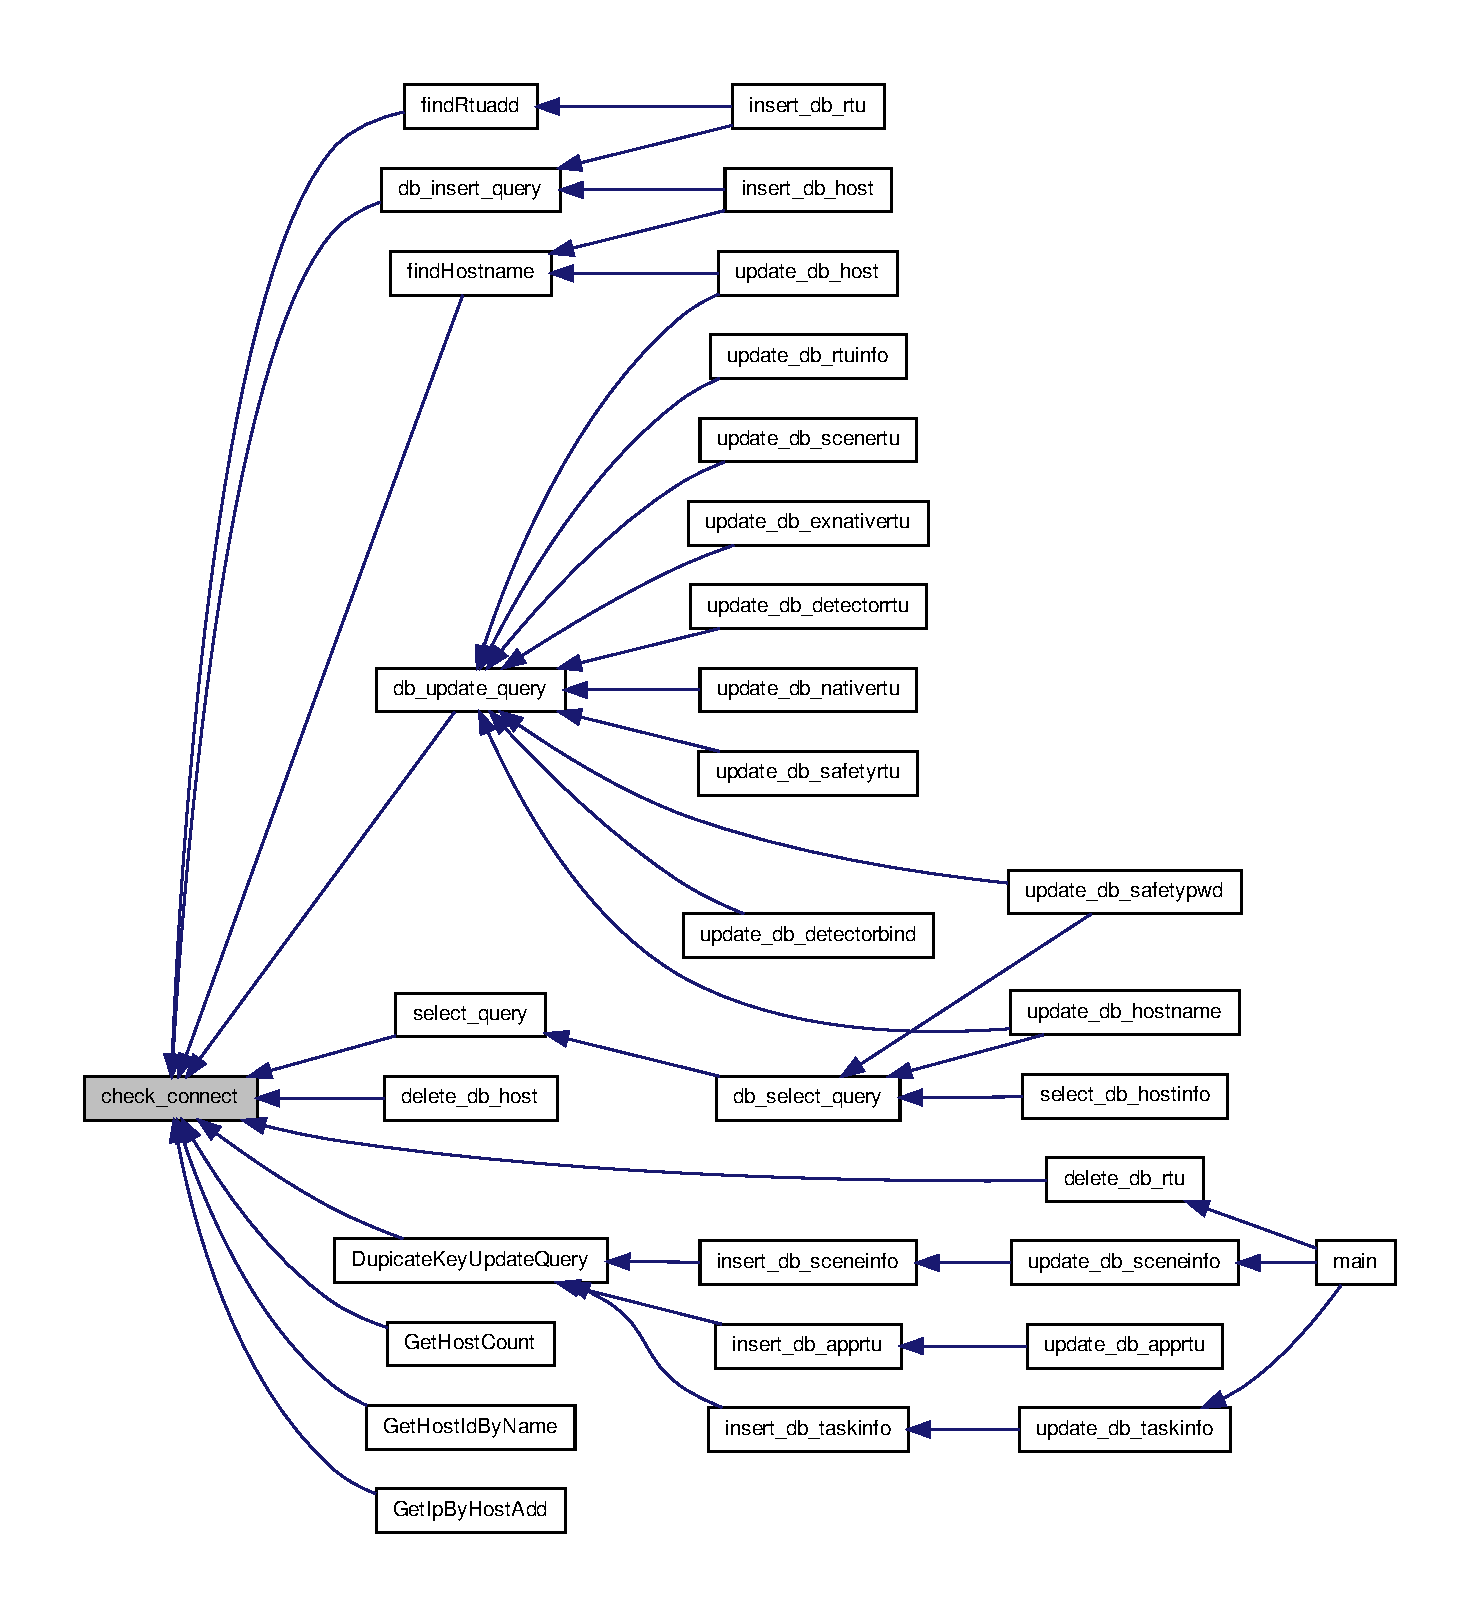
\includegraphics[width=350pt]{dbbase_8cpp_a45f3ac6076b939b77778a8d8a2aebde6_icgraph}
\end{center}
\end{figure}


\hypertarget{dbbase_8cpp_ae3ea82d0883ed39d63abe2f2e5cde42f}{\index{dbbase.\-cpp@{dbbase.\-cpp}!db\-\_\-insert\-\_\-query@{db\-\_\-insert\-\_\-query}}
\index{db\-\_\-insert\-\_\-query@{db\-\_\-insert\-\_\-query}!dbbase.cpp@{dbbase.\-cpp}}
\subsubsection[{db\-\_\-insert\-\_\-query}]{\setlength{\rightskip}{0pt plus 5cm}static int db\-\_\-insert\-\_\-query (
\begin{DoxyParamCaption}
\item[{const string \&}]{colstr, }
\item[{const string \&}]{valstr, }
\item[{const string \&}]{tablename}
\end{DoxyParamCaption}
)\hspace{0.3cm}{\ttfamily [static]}}}\label{dbbase_8cpp_ae3ea82d0883ed39d63abe2f2e5cde42f}


db\-\_\-insert\-\_\-query 数据库插入 


\begin{DoxyParams}{Parameters}
{\em colstr} & 列字段 \\
\hline
{\em valstr} & 值字段 \\
\hline
{\em tablename} & 数据表名\\
\hline
\end{DoxyParams}
\begin{DoxyReturn}{Returns}

\end{DoxyReturn}


References check\-\_\-connect(), insert\-\_\-mysql(), L\-O\-G\-\_\-\-D\-E\-B\-U\-G, and L\-O\-G\-\_\-\-E\-R\-R\-O\-R.



Referenced by insert\-\_\-db\-\_\-host(), and insert\-\_\-db\-\_\-rtu().



Here is the call graph for this function\-:\nopagebreak
\begin{figure}[H]
\begin{center}
\leavevmode
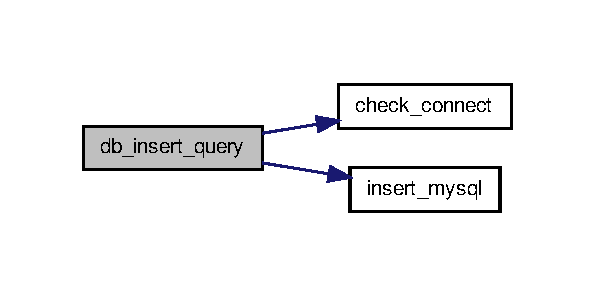
\includegraphics[width=286pt]{dbbase_8cpp_ae3ea82d0883ed39d63abe2f2e5cde42f_cgraph}
\end{center}
\end{figure}




Here is the caller graph for this function\-:\nopagebreak
\begin{figure}[H]
\begin{center}
\leavevmode
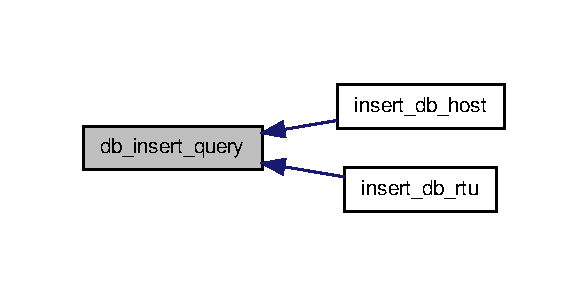
\includegraphics[width=282pt]{dbbase_8cpp_ae3ea82d0883ed39d63abe2f2e5cde42f_icgraph}
\end{center}
\end{figure}


\hypertarget{dbbase_8cpp_a7f355040a91d1275a6ac9a9490025717}{\index{dbbase.\-cpp@{dbbase.\-cpp}!db\-\_\-select\-\_\-query@{db\-\_\-select\-\_\-query}}
\index{db\-\_\-select\-\_\-query@{db\-\_\-select\-\_\-query}!dbbase.cpp@{dbbase.\-cpp}}
\subsubsection[{db\-\_\-select\-\_\-query}]{\setlength{\rightskip}{0pt plus 5cm}static {\bf Uint32} db\-\_\-select\-\_\-query (
\begin{DoxyParamCaption}
\item[{const string \&}]{colstr, }
\item[{const string \&}]{wheresrt, }
\item[{const string \&}]{tablename, }
\item[{string \&}]{retstr}
\end{DoxyParamCaption}
)\hspace{0.3cm}{\ttfamily [static]}}}\label{dbbase_8cpp_a7f355040a91d1275a6ac9a9490025717}


db\-\_\-select\-\_\-query 查找操作 


\begin{DoxyParams}{Parameters}
{\em colstr} & 列字段 \\
\hline
{\em wheresrt} & 过滤字段 \\
\hline
{\em tablename} & 表名 \\
\hline
{\em retstr} & 查找结果\\
\hline
\end{DoxyParams}
\begin{DoxyReturn}{Returns}

\end{DoxyReturn}


References L\-O\-G\-\_\-\-D\-E\-B\-U\-G, L\-O\-G\-\_\-\-E\-R\-R\-O\-R, and select\-\_\-query().



Referenced by select\-\_\-db\-\_\-hostinfo(), update\-\_\-db\-\_\-hostname(), and update\-\_\-db\-\_\-safetypwd().



Here is the call graph for this function\-:\nopagebreak
\begin{figure}[H]
\begin{center}
\leavevmode
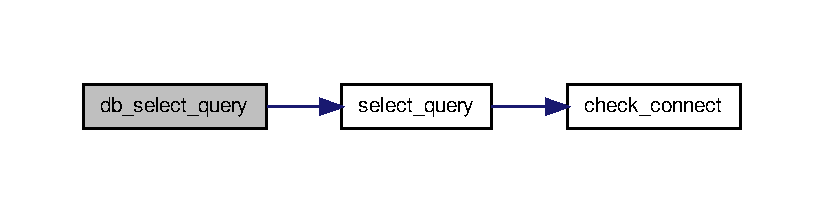
\includegraphics[width=350pt]{dbbase_8cpp_a7f355040a91d1275a6ac9a9490025717_cgraph}
\end{center}
\end{figure}




Here is the caller graph for this function\-:\nopagebreak
\begin{figure}[H]
\begin{center}
\leavevmode
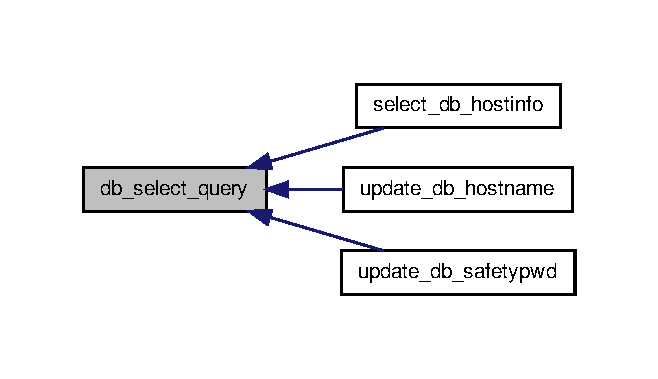
\includegraphics[width=316pt]{dbbase_8cpp_a7f355040a91d1275a6ac9a9490025717_icgraph}
\end{center}
\end{figure}


\hypertarget{dbbase_8cpp_a09e73ba1c0460f0f548fffa8f8aa8ebb}{\index{dbbase.\-cpp@{dbbase.\-cpp}!db\-\_\-update\-\_\-query@{db\-\_\-update\-\_\-query}}
\index{db\-\_\-update\-\_\-query@{db\-\_\-update\-\_\-query}!dbbase.cpp@{dbbase.\-cpp}}
\subsubsection[{db\-\_\-update\-\_\-query}]{\setlength{\rightskip}{0pt plus 5cm}static int db\-\_\-update\-\_\-query (
\begin{DoxyParamCaption}
\item[{const string \&}]{setstr, }
\item[{const string \&}]{wherestr, }
\item[{const string \&}]{tablename}
\end{DoxyParamCaption}
)\hspace{0.3cm}{\ttfamily [static]}}}\label{dbbase_8cpp_a09e73ba1c0460f0f548fffa8f8aa8ebb}


db\-\_\-update\-\_\-query 更新查询 


\begin{DoxyParams}{Parameters}
{\em setstr} & 设置字符串 \\
\hline
{\em wherestr} & 条件字符串 \\
\hline
{\em tablename} & 表名\\
\hline
\end{DoxyParams}
\begin{DoxyReturn}{Returns}

\end{DoxyReturn}


References check\-\_\-connect(), L\-O\-G\-\_\-\-D\-E\-B\-U\-G, and m\-\_\-mysqlfd.



Referenced by update\-\_\-db\-\_\-detectorbind(), update\-\_\-db\-\_\-detectorrtu(), update\-\_\-db\-\_\-exnativertu(), update\-\_\-db\-\_\-host(), update\-\_\-db\-\_\-hostname(), update\-\_\-db\-\_\-nativertu(), update\-\_\-db\-\_\-rtuinfo(), update\-\_\-db\-\_\-safetypwd(), update\-\_\-db\-\_\-safetyrtu(), and update\-\_\-db\-\_\-scenertu().



Here is the call graph for this function\-:\nopagebreak
\begin{figure}[H]
\begin{center}
\leavevmode
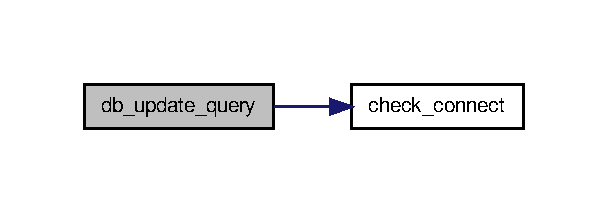
\includegraphics[width=292pt]{dbbase_8cpp_a09e73ba1c0460f0f548fffa8f8aa8ebb_cgraph}
\end{center}
\end{figure}




Here is the caller graph for this function\-:\nopagebreak
\begin{figure}[H]
\begin{center}
\leavevmode
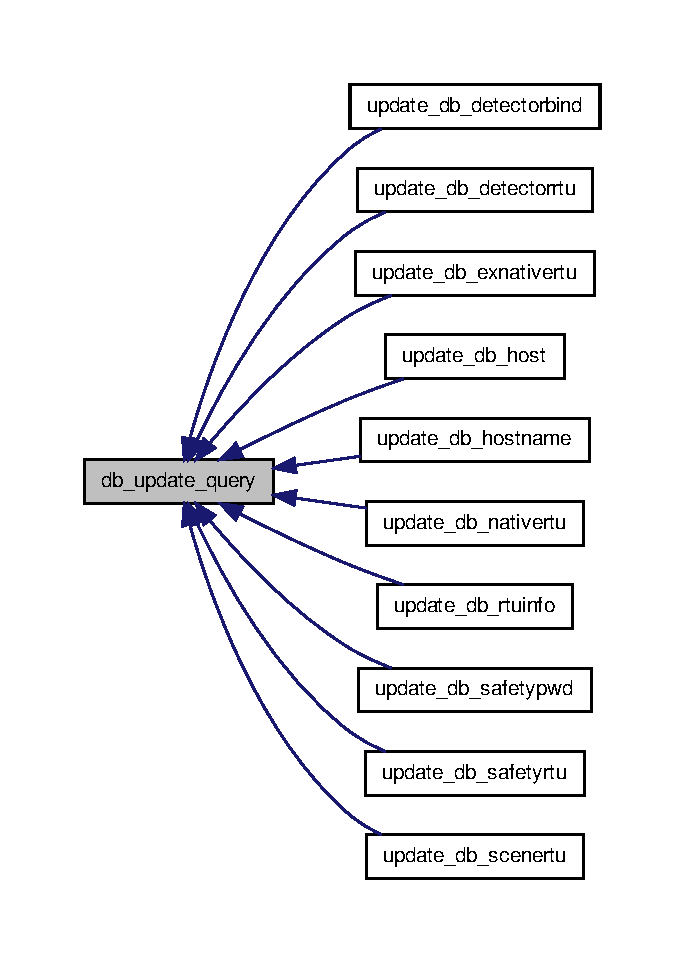
\includegraphics[width=328pt]{dbbase_8cpp_a09e73ba1c0460f0f548fffa8f8aa8ebb_icgraph}
\end{center}
\end{figure}


\hypertarget{dbbase_8cpp_a91ce6d4931baf0cca718619888e1412d}{\index{dbbase.\-cpp@{dbbase.\-cpp}!delete\-\_\-db\-\_\-host@{delete\-\_\-db\-\_\-host}}
\index{delete\-\_\-db\-\_\-host@{delete\-\_\-db\-\_\-host}!dbbase.cpp@{dbbase.\-cpp}}
\subsubsection[{delete\-\_\-db\-\_\-host}]{\setlength{\rightskip}{0pt plus 5cm}int delete\-\_\-db\-\_\-host (
\begin{DoxyParamCaption}
\item[{char $\ast$}]{hostname}
\end{DoxyParamCaption}
)}}\label{dbbase_8cpp_a91ce6d4931baf0cca718619888e1412d}


delete\-\_\-db\-\_\-host 删除主机设备 


\begin{DoxyParams}{Parameters}
{\em hostname} & 主机名 \\
\hline
\end{DoxyParams}
\begin{DoxyReturn}{Returns}

\end{DoxyReturn}


References check\-\_\-connect(), D\-B\-\_\-\-T\-A\-B\-L\-E\-\_\-\-N\-A\-M\-E\-L\-I\-S\-T, L\-O\-G\-\_\-\-D\-E\-B\-U\-G, L\-O\-G\-\_\-\-E\-R\-R\-O\-R, m\-\_\-mysqlfd, and M\-A\-X\-\_\-\-D\-B\-\_\-\-T\-Y\-P\-E.



Here is the call graph for this function\-:\nopagebreak
\begin{figure}[H]
\begin{center}
\leavevmode
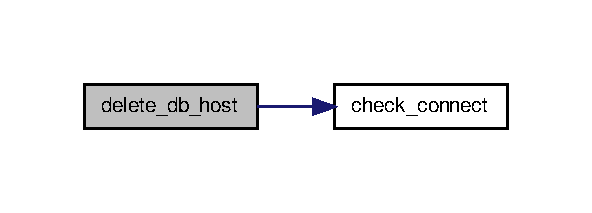
\includegraphics[width=284pt]{dbbase_8cpp_a91ce6d4931baf0cca718619888e1412d_cgraph}
\end{center}
\end{figure}


\hypertarget{dbbase_8cpp_adfa21954b5a414041dffb59dd549dcb8}{\index{dbbase.\-cpp@{dbbase.\-cpp}!delete\-\_\-db\-\_\-rtu@{delete\-\_\-db\-\_\-rtu}}
\index{delete\-\_\-db\-\_\-rtu@{delete\-\_\-db\-\_\-rtu}!dbbase.cpp@{dbbase.\-cpp}}
\subsubsection[{delete\-\_\-db\-\_\-rtu}]{\setlength{\rightskip}{0pt plus 5cm}int delete\-\_\-db\-\_\-rtu (
\begin{DoxyParamCaption}
\item[{{\bf Rtu\-Remove\-Info} \&}]{rtuinfo}
\end{DoxyParamCaption}
)}}\label{dbbase_8cpp_adfa21954b5a414041dffb59dd549dcb8}


delete\-\_\-db\-\_\-rtu 删除设备 接口 不包括删除主机 


\begin{DoxyParams}{Parameters}
{\em rtuinfo} & \\
\hline
\end{DoxyParams}
\begin{DoxyReturn}{Returns}
-\/1 删除出错 0 删除成功 或者 没有删除项 
\end{DoxyReturn}


References check\-\_\-connect(), get\-\_\-table\-\_\-name(), Rtu\-Remove\-Info\-::hostadd, L\-O\-G\-\_\-\-D\-E\-B\-U\-G, L\-O\-G\-\_\-\-E\-R\-R\-O\-R, m\-\_\-mysqlfd, Rtu\-Remove\-Info\-::rtuadd, and Rtu\-Remove\-Info\-::rtutype.



Referenced by main().



Here is the call graph for this function\-:\nopagebreak
\begin{figure}[H]
\begin{center}
\leavevmode
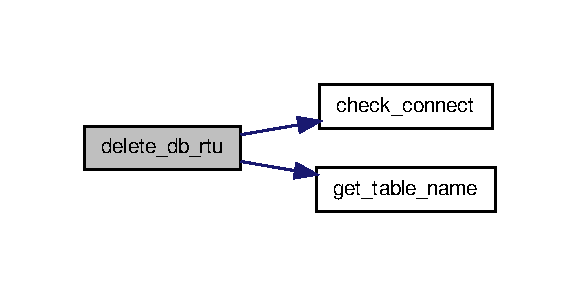
\includegraphics[width=278pt]{dbbase_8cpp_adfa21954b5a414041dffb59dd549dcb8_cgraph}
\end{center}
\end{figure}




Here is the caller graph for this function\-:\nopagebreak
\begin{figure}[H]
\begin{center}
\leavevmode
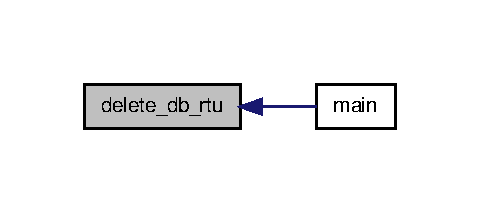
\includegraphics[width=230pt]{dbbase_8cpp_adfa21954b5a414041dffb59dd549dcb8_icgraph}
\end{center}
\end{figure}


\hypertarget{dbbase_8cpp_ac9d1db67754ebd6ac53cd4ce185a22cd}{\index{dbbase.\-cpp@{dbbase.\-cpp}!Dupicate\-Key\-Update\-Query@{Dupicate\-Key\-Update\-Query}}
\index{Dupicate\-Key\-Update\-Query@{Dupicate\-Key\-Update\-Query}!dbbase.cpp@{dbbase.\-cpp}}
\subsubsection[{Dupicate\-Key\-Update\-Query}]{\setlength{\rightskip}{0pt plus 5cm}static int Dupicate\-Key\-Update\-Query (
\begin{DoxyParamCaption}
\item[{const string \&}]{colstr, }
\item[{const string \&}]{valstr, }
\item[{const string \&}]{updatestr, }
\item[{const string \&}]{tablename}
\end{DoxyParamCaption}
)\hspace{0.3cm}{\ttfamily [static]}}}\label{dbbase_8cpp_ac9d1db67754ebd6ac53cd4ce185a22cd}


Dupicate\-Key\-Update\-Query 更新、插入查询:存在则更新不存在则插入 


\begin{DoxyParams}{Parameters}
{\em colstr} & 列 \\
\hline
{\em valstr} & 值 \\
\hline
{\em updatestr} & 要更新的列 \\
\hline
{\em tablename} & 表名\\
\hline
\end{DoxyParams}
\begin{DoxyReturn}{Returns}

\end{DoxyReturn}


References check\-\_\-connect(), L\-O\-G\-\_\-\-D\-E\-B\-U\-G, and m\-\_\-mysqlfd.



Referenced by insert\-\_\-db\-\_\-apprtu(), insert\-\_\-db\-\_\-sceneinfo(), and insert\-\_\-db\-\_\-taskinfo().



Here is the call graph for this function\-:\nopagebreak
\begin{figure}[H]
\begin{center}
\leavevmode
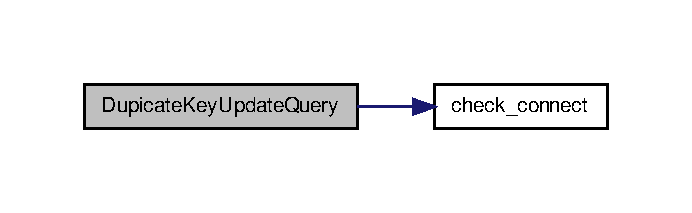
\includegraphics[width=332pt]{dbbase_8cpp_ac9d1db67754ebd6ac53cd4ce185a22cd_cgraph}
\end{center}
\end{figure}




Here is the caller graph for this function\-:\nopagebreak
\begin{figure}[H]
\begin{center}
\leavevmode
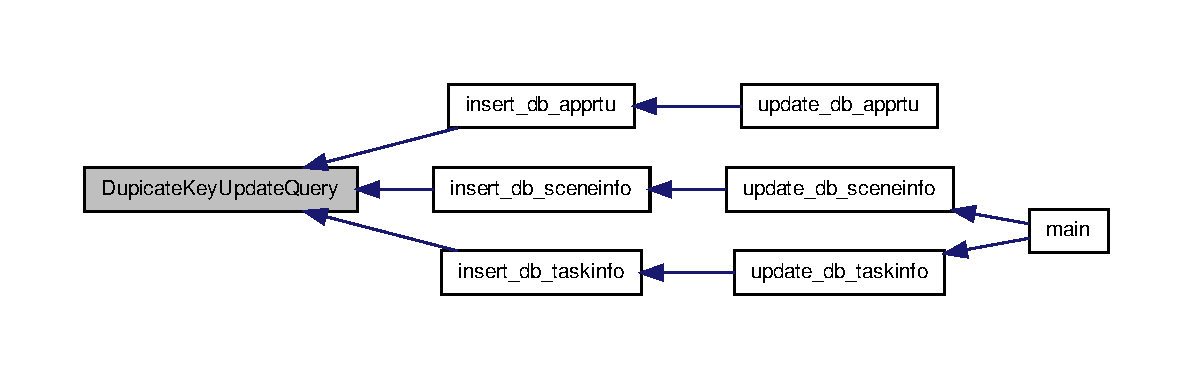
\includegraphics[width=350pt]{dbbase_8cpp_ac9d1db67754ebd6ac53cd4ce185a22cd_icgraph}
\end{center}
\end{figure}


\hypertarget{dbbase_8cpp_a7748ddce59655cc11534b75d5e0956d4}{\index{dbbase.\-cpp@{dbbase.\-cpp}!find\-Hostname@{find\-Hostname}}
\index{find\-Hostname@{find\-Hostname}!dbbase.cpp@{dbbase.\-cpp}}
\subsubsection[{find\-Hostname}]{\setlength{\rightskip}{0pt plus 5cm}int find\-Hostname (
\begin{DoxyParamCaption}
\item[{char $\ast$}]{hostname}
\end{DoxyParamCaption}
)}}\label{dbbase_8cpp_a7748ddce59655cc11534b75d5e0956d4}


find\-Hostname 查找对应的主机名 


\begin{DoxyParams}{Parameters}
{\em hostname} & 主机名\\
\hline
\end{DoxyParams}
\begin{DoxyReturn}{Returns}
返回值 -\/1 错误 0 没有找到对应的 $>$0 找到的主机个数 
\end{DoxyReturn}


References check\-\_\-connect(), L\-O\-G\-\_\-\-E\-R\-R\-O\-R, and m\-\_\-mysqlfd.



Referenced by insert\-\_\-db\-\_\-host(), and update\-\_\-db\-\_\-host().



Here is the call graph for this function\-:\nopagebreak
\begin{figure}[H]
\begin{center}
\leavevmode
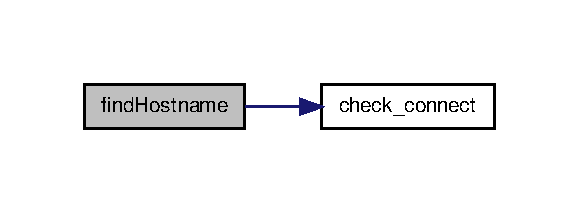
\includegraphics[width=278pt]{dbbase_8cpp_a7748ddce59655cc11534b75d5e0956d4_cgraph}
\end{center}
\end{figure}




Here is the caller graph for this function\-:\nopagebreak
\begin{figure}[H]
\begin{center}
\leavevmode
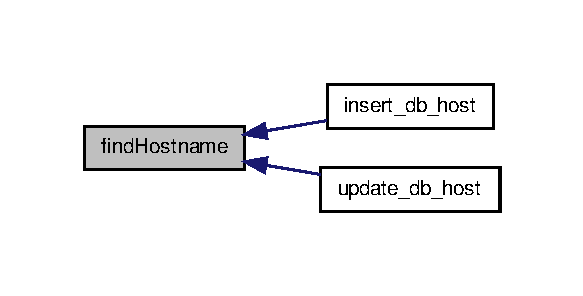
\includegraphics[width=280pt]{dbbase_8cpp_a7748ddce59655cc11534b75d5e0956d4_icgraph}
\end{center}
\end{figure}


\hypertarget{dbbase_8cpp_aec7bbc2b50281d325bd7e99661ef5c60}{\index{dbbase.\-cpp@{dbbase.\-cpp}!find\-Rtuadd@{find\-Rtuadd}}
\index{find\-Rtuadd@{find\-Rtuadd}!dbbase.cpp@{dbbase.\-cpp}}
\subsubsection[{find\-Rtuadd}]{\setlength{\rightskip}{0pt plus 5cm}static int find\-Rtuadd (
\begin{DoxyParamCaption}
\item[{{\bf Uint32}}]{rtuadd, }
\item[{const string \&}]{tablename}
\end{DoxyParamCaption}
)\hspace{0.3cm}{\ttfamily [static]}}}\label{dbbase_8cpp_aec7bbc2b50281d325bd7e99661ef5c60}
查看对应的设备是否已经存在 

References check\-\_\-connect(), L\-O\-G\-\_\-\-E\-R\-R\-O\-R, and m\-\_\-mysqlfd.



Referenced by insert\-\_\-db\-\_\-rtu().



Here is the call graph for this function\-:\nopagebreak
\begin{figure}[H]
\begin{center}
\leavevmode
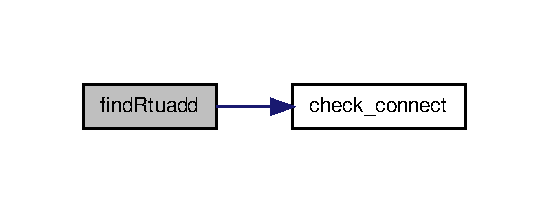
\includegraphics[width=264pt]{dbbase_8cpp_aec7bbc2b50281d325bd7e99661ef5c60_cgraph}
\end{center}
\end{figure}




Here is the caller graph for this function\-:\nopagebreak
\begin{figure}[H]
\begin{center}
\leavevmode
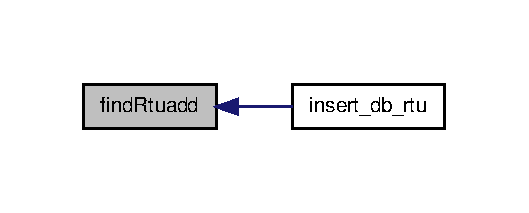
\includegraphics[width=254pt]{dbbase_8cpp_aec7bbc2b50281d325bd7e99661ef5c60_icgraph}
\end{center}
\end{figure}


\hypertarget{dbbase_8cpp_af89ddd8c208010e4477750f84849f9bf}{\index{dbbase.\-cpp@{dbbase.\-cpp}!get\-\_\-table\-\_\-name@{get\-\_\-table\-\_\-name}}
\index{get\-\_\-table\-\_\-name@{get\-\_\-table\-\_\-name}!dbbase.cpp@{dbbase.\-cpp}}
\subsubsection[{get\-\_\-table\-\_\-name}]{\setlength{\rightskip}{0pt plus 5cm}std\-::string get\-\_\-table\-\_\-name (
\begin{DoxyParamCaption}
\item[{{\bf Uint8}}]{type}
\end{DoxyParamCaption}
)}}\label{dbbase_8cpp_af89ddd8c208010e4477750f84849f9bf}


get\-\_\-table\-\_\-name 根据设备类型 拿到对应的表名 


\begin{DoxyParams}{Parameters}
{\em type} & 设备类型 \\
\hline
\end{DoxyParams}
\begin{DoxyReturn}{Returns}
表名 为 string 类型 
\end{DoxyReturn}


References g\-Type\-Info\-List, and D\-B\-Type\-Info\-::tablename.



Referenced by delete\-\_\-db\-\_\-rtu(), insert\-\_\-db\-\_\-rtu(), update\-\_\-db\-\_\-exnativertu(), update\-\_\-db\-\_\-host(), update\-\_\-db\-\_\-rtuinfo(), and update\-\_\-db\-\_\-safetyrtu().



Here is the caller graph for this function\-:\nopagebreak
\begin{figure}[H]
\begin{center}
\leavevmode
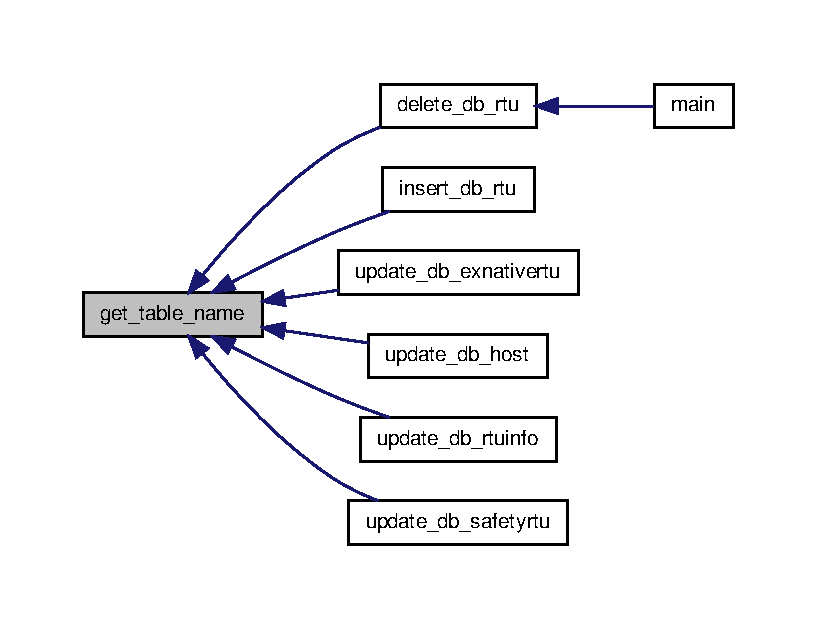
\includegraphics[width=350pt]{dbbase_8cpp_af89ddd8c208010e4477750f84849f9bf_icgraph}
\end{center}
\end{figure}


\hypertarget{dbbase_8cpp_a45ba5638ae09b4ccca4dbe1bdb6bf89a}{\index{dbbase.\-cpp@{dbbase.\-cpp}!Get\-Host\-Count@{Get\-Host\-Count}}
\index{Get\-Host\-Count@{Get\-Host\-Count}!dbbase.cpp@{dbbase.\-cpp}}
\subsubsection[{Get\-Host\-Count}]{\setlength{\rightskip}{0pt plus 5cm}int Get\-Host\-Count (
\begin{DoxyParamCaption}
{}
\end{DoxyParamCaption}
)}}\label{dbbase_8cpp_a45ba5638ae09b4ccca4dbe1bdb6bf89a}


Get\-Host\-Count 拿到 连接上来的主机个数 

\begin{DoxyReturn}{Returns}
主机个数 
\end{DoxyReturn}


References check\-\_\-connect(), L\-O\-G\-\_\-\-D\-E\-B\-U\-G, L\-O\-G\-\_\-\-E\-R\-R\-O\-R, and m\-\_\-mysqlfd.



Here is the call graph for this function\-:\nopagebreak
\begin{figure}[H]
\begin{center}
\leavevmode
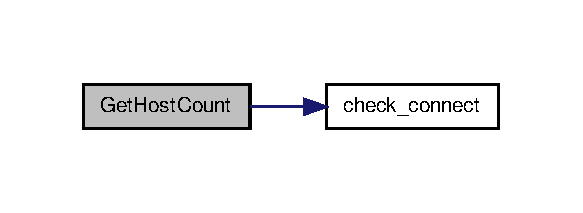
\includegraphics[width=280pt]{dbbase_8cpp_a45ba5638ae09b4ccca4dbe1bdb6bf89a_cgraph}
\end{center}
\end{figure}


\hypertarget{dbbase_8cpp_a645417f4347afad166d95e919bf778de}{\index{dbbase.\-cpp@{dbbase.\-cpp}!Get\-Host\-Id\-By\-Name@{Get\-Host\-Id\-By\-Name}}
\index{Get\-Host\-Id\-By\-Name@{Get\-Host\-Id\-By\-Name}!dbbase.cpp@{dbbase.\-cpp}}
\subsubsection[{Get\-Host\-Id\-By\-Name}]{\setlength{\rightskip}{0pt plus 5cm}{\bf Uint32} Get\-Host\-Id\-By\-Name (
\begin{DoxyParamCaption}
\item[{char $\ast$}]{hostname, }
\item[{{\bf Uint32} \&}]{hostid}
\end{DoxyParamCaption}
)}}\label{dbbase_8cpp_a645417f4347afad166d95e919bf778de}


Get\-Host\-Id\-By\-Name 根据主机名查找对应的\-I\-D. 


\begin{DoxyParams}{Parameters}
{\em hostname} & 主机名 \\
\hline
{\em hostid} & 找到的hostadd放入该参数\\
\hline
\end{DoxyParams}
\begin{DoxyReturn}{Returns}
-\/1 查找错误 0 查找正确 
\end{DoxyReturn}


References check\-\_\-connect(), L\-O\-G\-\_\-\-D\-E\-B\-U\-G, L\-O\-G\-\_\-\-E\-R\-R\-O\-R, and m\-\_\-mysqlfd.



Here is the call graph for this function\-:\nopagebreak
\begin{figure}[H]
\begin{center}
\leavevmode
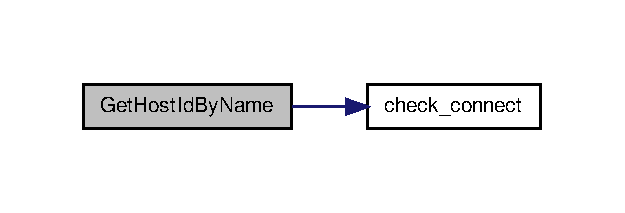
\includegraphics[width=300pt]{dbbase_8cpp_a645417f4347afad166d95e919bf778de_cgraph}
\end{center}
\end{figure}


\hypertarget{dbbase_8cpp_aa1165b8a3c5a7d095576c678f94268f3}{\index{dbbase.\-cpp@{dbbase.\-cpp}!Get\-Ip\-By\-Host\-Add@{Get\-Ip\-By\-Host\-Add}}
\index{Get\-Ip\-By\-Host\-Add@{Get\-Ip\-By\-Host\-Add}!dbbase.cpp@{dbbase.\-cpp}}
\subsubsection[{Get\-Ip\-By\-Host\-Add}]{\setlength{\rightskip}{0pt plus 5cm}{\bf Uint32} Get\-Ip\-By\-Host\-Add (
\begin{DoxyParamCaption}
\item[{{\bf Uint32}}]{hostadd, }
\item[{{\bf Uint32} \&}]{hostip}
\end{DoxyParamCaption}
)}}\label{dbbase_8cpp_aa1165b8a3c5a7d095576c678f94268f3}
根据 hostadd 拿到 ip 

References check\-\_\-connect(), L\-O\-G\-\_\-\-D\-E\-B\-U\-G, L\-O\-G\-\_\-\-E\-R\-R\-O\-R, and m\-\_\-mysqlfd.



Here is the call graph for this function\-:\nopagebreak
\begin{figure}[H]
\begin{center}
\leavevmode
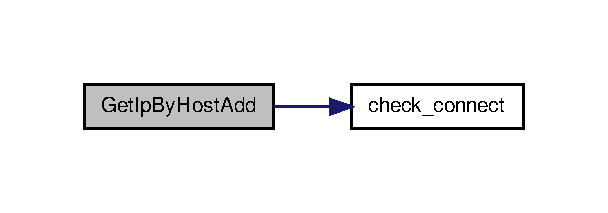
\includegraphics[width=292pt]{dbbase_8cpp_aa1165b8a3c5a7d095576c678f94268f3_cgraph}
\end{center}
\end{figure}


\hypertarget{dbbase_8cpp_affefb171c935f2ae5832d0ca8091798f}{\index{dbbase.\-cpp@{dbbase.\-cpp}!init\-\_\-mysql@{init\-\_\-mysql}}
\index{init\-\_\-mysql@{init\-\_\-mysql}!dbbase.cpp@{dbbase.\-cpp}}
\subsubsection[{init\-\_\-mysql}]{\setlength{\rightskip}{0pt plus 5cm}int init\-\_\-mysql (
\begin{DoxyParamCaption}
\item[{{\bf Mysql\-Con\-Info} $\ast$}]{info}
\end{DoxyParamCaption}
)}}\label{dbbase_8cpp_affefb171c935f2ae5832d0ca8091798f}


init\-\_\-mysql 初始化mysql , 连接,指定数据库 


\begin{DoxyParams}{Parameters}
{\em info} & 连接mysql时,mysql相关信息结构体\\
\hline
\end{DoxyParams}
\begin{DoxyReturn}{Returns}
0 成功 -\/1 失败 
\end{DoxyReturn}


References Mysql\-Con\-Info\-::dbname, Mysql\-Con\-Info\-::hostname, m\-\_\-mysqlfd, Mysql\-Con\-Info\-::password, and Mysql\-Con\-Info\-::username.



Referenced by main().



Here is the caller graph for this function\-:\nopagebreak
\begin{figure}[H]
\begin{center}
\leavevmode
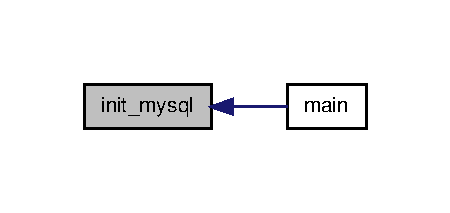
\includegraphics[width=216pt]{dbbase_8cpp_affefb171c935f2ae5832d0ca8091798f_icgraph}
\end{center}
\end{figure}


\hypertarget{dbbase_8cpp_a62123b0c0b89cfe644b8e040a4fe2a3b}{\index{dbbase.\-cpp@{dbbase.\-cpp}!insert\-\_\-db\-\_\-apprtu@{insert\-\_\-db\-\_\-apprtu}}
\index{insert\-\_\-db\-\_\-apprtu@{insert\-\_\-db\-\_\-apprtu}!dbbase.cpp@{dbbase.\-cpp}}
\subsubsection[{insert\-\_\-db\-\_\-apprtu}]{\setlength{\rightskip}{0pt plus 5cm}int insert\-\_\-db\-\_\-apprtu (
\begin{DoxyParamCaption}
\item[{{\bf App\-Rtu\-Info} \&}]{rtuinfo}
\end{DoxyParamCaption}
)}}\label{dbbase_8cpp_a62123b0c0b89cfe644b8e040a4fe2a3b}


insert\-\_\-db\-\_\-apprtu 添加,编辑 应用设备 


\begin{DoxyParams}{Parameters}
{\em rtuinfo} & 应用设备结构体\\
\hline
\end{DoxyParams}
\begin{DoxyReturn}{Returns}

\end{DoxyReturn}


References D\-B\-\_\-\-T\-A\-B\-L\-E\-\_\-\-N\-A\-M\-E\-L\-I\-S\-T, Dupicate\-Key\-Update\-Query(), App\-Rtu\-Info\-::hostadd, App\-Rtu\-Info\-::irrtuadd, L\-O\-G\-\_\-\-E\-R\-R\-O\-R, R\-T\-U\-\_\-\-S\-T\-A\-T\-E\-\_\-\-V\-A\-L\-I\-D, App\-Rtu\-Info\-::rtuadd, App\-Rtu\-Info\-::rtuname, App\-Rtu\-Info\-::rturegtime, and App\-Rtu\-Info\-::rtutype.



Referenced by update\-\_\-db\-\_\-apprtu().



Here is the call graph for this function\-:\nopagebreak
\begin{figure}[H]
\begin{center}
\leavevmode
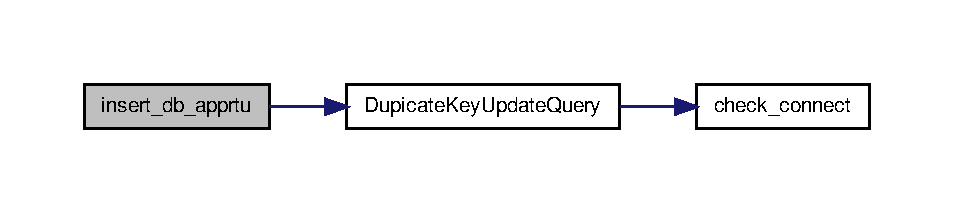
\includegraphics[width=350pt]{dbbase_8cpp_a62123b0c0b89cfe644b8e040a4fe2a3b_cgraph}
\end{center}
\end{figure}




Here is the caller graph for this function\-:\nopagebreak
\begin{figure}[H]
\begin{center}
\leavevmode
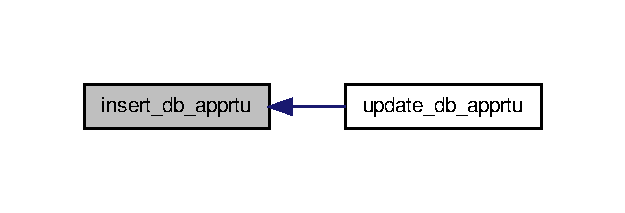
\includegraphics[width=300pt]{dbbase_8cpp_a62123b0c0b89cfe644b8e040a4fe2a3b_icgraph}
\end{center}
\end{figure}


\hypertarget{dbbase_8cpp_a9acb52e4299badf813180da0f8214c37}{\index{dbbase.\-cpp@{dbbase.\-cpp}!insert\-\_\-db\-\_\-host@{insert\-\_\-db\-\_\-host}}
\index{insert\-\_\-db\-\_\-host@{insert\-\_\-db\-\_\-host}!dbbase.cpp@{dbbase.\-cpp}}
\subsubsection[{insert\-\_\-db\-\_\-host}]{\setlength{\rightskip}{0pt plus 5cm}int insert\-\_\-db\-\_\-host (
\begin{DoxyParamCaption}
\item[{{\bf Host\-Reg\-Info} \&}]{hostinfo}
\end{DoxyParamCaption}
)}}\label{dbbase_8cpp_a9acb52e4299badf813180da0f8214c37}


insert\-\_\-db\-\_\-host 主机注册接口 


\begin{DoxyParams}{Parameters}
{\em hostinfo} & 主机信息结构体\\
\hline
\end{DoxyParams}
\begin{DoxyReturn}{Returns}
-\/1 插入失败 0 插入成功 $>$0 主机名字已经存在 
\end{DoxyReturn}


References db\-\_\-insert\-\_\-query(), D\-B\-\_\-\-T\-A\-B\-L\-E\-\_\-\-N\-A\-M\-E\-L\-I\-S\-T, find\-Hostname(), Host\-Reg\-Info\-::hostadd, Host\-Reg\-Info\-::hostip, Host\-Reg\-Info\-::hostname, Host\-Reg\-Info\-::hostpwd, Host\-Reg\-Info\-::hostregtime, Host\-Reg\-Info\-::lastcomtime, L\-O\-G\-\_\-\-E\-R\-R\-O\-R, L\-O\-G\-\_\-\-P\-R\-I\-N\-T, and R\-T\-U\-\_\-\-S\-T\-A\-T\-E\-\_\-\-V\-A\-L\-I\-D.



Here is the call graph for this function\-:\nopagebreak
\begin{figure}[H]
\begin{center}
\leavevmode
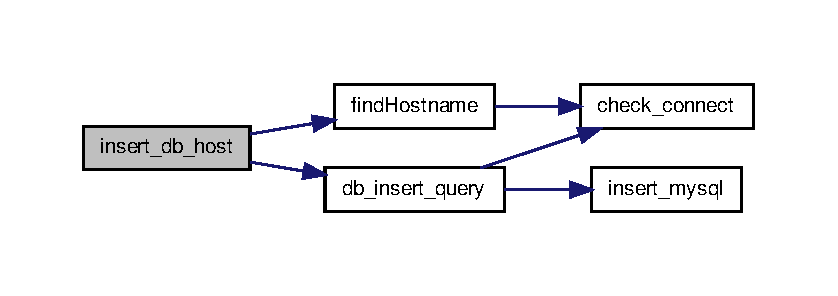
\includegraphics[width=350pt]{dbbase_8cpp_a9acb52e4299badf813180da0f8214c37_cgraph}
\end{center}
\end{figure}


\hypertarget{dbbase_8cpp_a21f3b1ac4424fa0839c3182b0ab7cbd8}{\index{dbbase.\-cpp@{dbbase.\-cpp}!insert\-\_\-db\-\_\-rtu@{insert\-\_\-db\-\_\-rtu}}
\index{insert\-\_\-db\-\_\-rtu@{insert\-\_\-db\-\_\-rtu}!dbbase.cpp@{dbbase.\-cpp}}
\subsubsection[{insert\-\_\-db\-\_\-rtu}]{\setlength{\rightskip}{0pt plus 5cm}int insert\-\_\-db\-\_\-rtu (
\begin{DoxyParamCaption}
\item[{{\bf Rtu\-Reg\-Info} \&}]{rtuinfo}
\end{DoxyParamCaption}
)}}\label{dbbase_8cpp_a21f3b1ac4424fa0839c3182b0ab7cbd8}


insert\-\_\-db\-\_\-rtu 注册设备接口 ,将设备写入数据库 


\begin{DoxyParams}{Parameters}
{\em rtuinfo} & 插入设备结构体\\
\hline
\end{DoxyParams}
\begin{DoxyReturn}{Returns}
-\/1 插入失败 0 插入成功 
\end{DoxyReturn}


References db\-\_\-insert\-\_\-query(), D\-B\-\_\-\-T\-A\-B\-L\-E\-\_\-\-N\-A\-M\-E\-L\-I\-S\-T, find\-Rtuadd(), get\-\_\-table\-\_\-name(), Rtu\-Reg\-Info\-::hostadd, L\-O\-G\-\_\-\-E\-R\-R\-O\-R, m\-\_\-mysqlfd, Rtu\-Reg\-Info\-::rtuadd, Rtu\-Reg\-Info\-::rturegtime, Rtu\-Reg\-Info\-::rtustate, and Rtu\-Reg\-Info\-::rtutype.



Here is the call graph for this function\-:\nopagebreak
\begin{figure}[H]
\begin{center}
\leavevmode
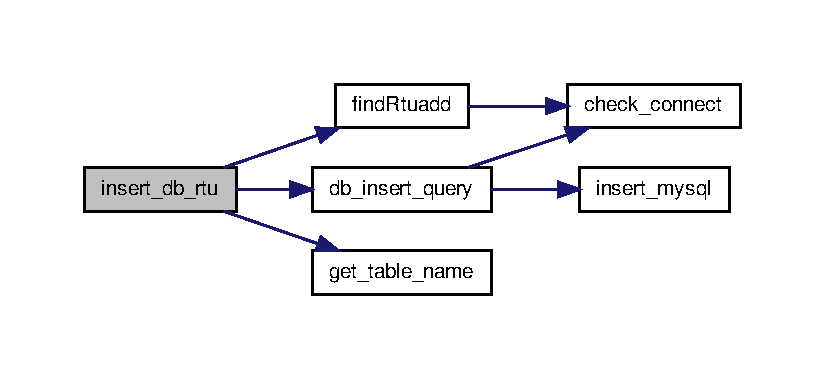
\includegraphics[width=350pt]{dbbase_8cpp_a21f3b1ac4424fa0839c3182b0ab7cbd8_cgraph}
\end{center}
\end{figure}


\hypertarget{dbbase_8cpp_ad9cd8d3ab8c7385eceb3280b5f910b2a}{\index{dbbase.\-cpp@{dbbase.\-cpp}!insert\-\_\-db\-\_\-sceneinfo@{insert\-\_\-db\-\_\-sceneinfo}}
\index{insert\-\_\-db\-\_\-sceneinfo@{insert\-\_\-db\-\_\-sceneinfo}!dbbase.cpp@{dbbase.\-cpp}}
\subsubsection[{insert\-\_\-db\-\_\-sceneinfo}]{\setlength{\rightskip}{0pt plus 5cm}int insert\-\_\-db\-\_\-sceneinfo (
\begin{DoxyParamCaption}
\item[{{\bf Scene\-Info} \&}]{sceneinfo}
\end{DoxyParamCaption}
)}}\label{dbbase_8cpp_ad9cd8d3ab8c7385eceb3280b5f910b2a}


insert\-\_\-db\-\_\-sceneinfo 创建、修改情景 


\begin{DoxyParams}{Parameters}
{\em sceneinfo} & 情景信息结构体 绑定的设备信息需要malloc后传入\\
\hline
\end{DoxyParams}
\begin{DoxyReturn}{Returns}

\end{DoxyReturn}


References Rtu\-Bind\-::add, D\-B\-\_\-\-T\-A\-B\-L\-E\-\_\-\-N\-A\-M\-E\-L\-I\-S\-T, Rtu\-Bind\-::delay, Dupicate\-Key\-Update\-Query(), Scene\-Info\-::hostadd, L\-O\-G\-\_\-\-E\-R\-R\-O\-R, Rtu\-Bind\-::oper, Scene\-Info\-::rtubind, Scene\-Info\-::rturegtime, Scene\-Info\-::sceneid, Scene\-Info\-::scenename, Scene\-Info\-::scenepicid, Scene\-Info\-::scenertunum, and Rtu\-Bind\-::type.



Referenced by update\-\_\-db\-\_\-sceneinfo().



Here is the call graph for this function\-:\nopagebreak
\begin{figure}[H]
\begin{center}
\leavevmode
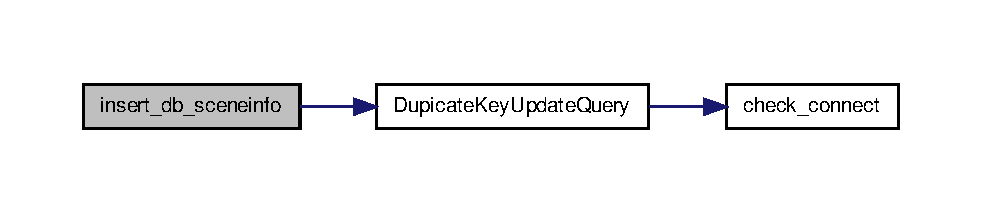
\includegraphics[width=350pt]{dbbase_8cpp_ad9cd8d3ab8c7385eceb3280b5f910b2a_cgraph}
\end{center}
\end{figure}




Here is the caller graph for this function\-:\nopagebreak
\begin{figure}[H]
\begin{center}
\leavevmode
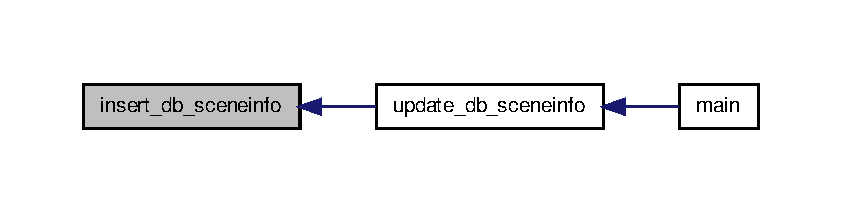
\includegraphics[width=350pt]{dbbase_8cpp_ad9cd8d3ab8c7385eceb3280b5f910b2a_icgraph}
\end{center}
\end{figure}


\hypertarget{dbbase_8cpp_a0eb771b638f26a87a9cce0c7de472f0f}{\index{dbbase.\-cpp@{dbbase.\-cpp}!insert\-\_\-db\-\_\-taskinfo@{insert\-\_\-db\-\_\-taskinfo}}
\index{insert\-\_\-db\-\_\-taskinfo@{insert\-\_\-db\-\_\-taskinfo}!dbbase.cpp@{dbbase.\-cpp}}
\subsubsection[{insert\-\_\-db\-\_\-taskinfo}]{\setlength{\rightskip}{0pt plus 5cm}int insert\-\_\-db\-\_\-taskinfo (
\begin{DoxyParamCaption}
\item[{{\bf Task\-Info} \&}]{taskinfo}
\end{DoxyParamCaption}
)}}\label{dbbase_8cpp_a0eb771b638f26a87a9cce0c7de472f0f}


insert\-\_\-db\-\_\-taskinfo 设置 编辑定时任务 


\begin{DoxyParams}{Parameters}
{\em taskinfo} & 任务信息 绑定的设备信息需要malloc后传入 \\
\hline
\end{DoxyParams}


References Rtu\-Bind\-::add, D\-B\-\_\-\-T\-A\-B\-L\-E\-\_\-\-N\-A\-M\-E\-L\-I\-S\-T, Rtu\-Bind\-::delay, Dupicate\-Key\-Update\-Query(), Task\-Info\-::hostadd, L\-O\-G\-\_\-\-E\-R\-R\-O\-R, Rtu\-Bind\-::oper, Task\-Info\-::rtubind, Task\-Info\-::taskcycle, Task\-Info\-::taskid, Task\-Info\-::taskname, Task\-Info\-::taskpicid, Task\-Info\-::taskregtime, Task\-Info\-::taskrtunum, Task\-Info\-::taskstdtime, and Rtu\-Bind\-::type.



Referenced by update\-\_\-db\-\_\-taskinfo().



Here is the call graph for this function\-:\nopagebreak
\begin{figure}[H]
\begin{center}
\leavevmode
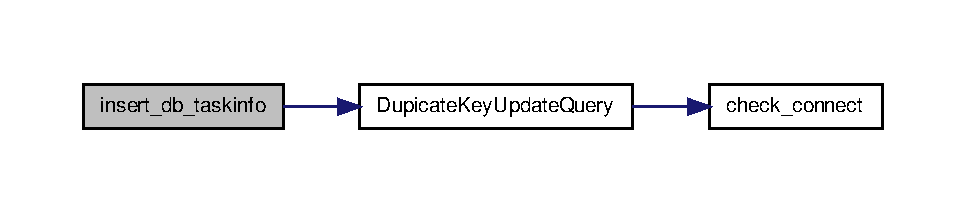
\includegraphics[width=350pt]{dbbase_8cpp_a0eb771b638f26a87a9cce0c7de472f0f_cgraph}
\end{center}
\end{figure}




Here is the caller graph for this function\-:\nopagebreak
\begin{figure}[H]
\begin{center}
\leavevmode
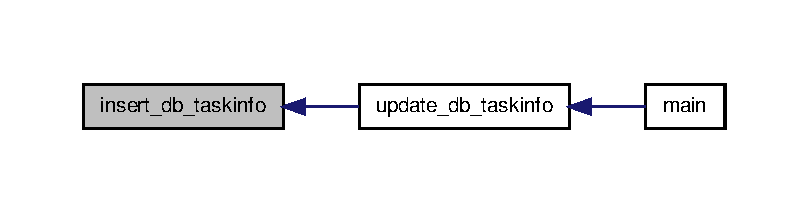
\includegraphics[width=350pt]{dbbase_8cpp_a0eb771b638f26a87a9cce0c7de472f0f_icgraph}
\end{center}
\end{figure}


\hypertarget{dbbase_8cpp_afe0ea3530d4cbbbf870292d37df7ac9e}{\index{dbbase.\-cpp@{dbbase.\-cpp}!insert\-\_\-mysql@{insert\-\_\-mysql}}
\index{insert\-\_\-mysql@{insert\-\_\-mysql}!dbbase.cpp@{dbbase.\-cpp}}
\subsubsection[{insert\-\_\-mysql}]{\setlength{\rightskip}{0pt plus 5cm}static int insert\-\_\-mysql (
\begin{DoxyParamCaption}
\item[{string}]{sql\-\_\-cmd}
\end{DoxyParamCaption}
)\hspace{0.3cm}{\ttfamily [static]}}}\label{dbbase_8cpp_afe0ea3530d4cbbbf870292d37df7ac9e}


insert\-\_\-mysql 数据库基本插入操作 


\begin{DoxyParams}{Parameters}
{\em sql\-\_\-cmd} & 插入命令 为string 类型 \\
\hline
\end{DoxyParams}
\begin{DoxyReturn}{Returns}

\end{DoxyReturn}


References L\-O\-G\-\_\-\-E\-R\-R\-O\-R, and m\-\_\-mysqlfd.



Referenced by db\-\_\-insert\-\_\-query().



Here is the caller graph for this function\-:\nopagebreak
\begin{figure}[H]
\begin{center}
\leavevmode
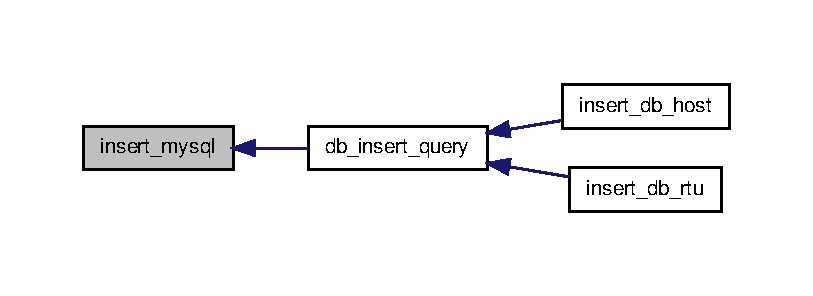
\includegraphics[width=350pt]{dbbase_8cpp_afe0ea3530d4cbbbf870292d37df7ac9e_icgraph}
\end{center}
\end{figure}


\hypertarget{dbbase_8cpp_a55f5cb081a0fc3774070718f283746d6}{\index{dbbase.\-cpp@{dbbase.\-cpp}!Is\-Native\-Rtu@{Is\-Native\-Rtu}}
\index{Is\-Native\-Rtu@{Is\-Native\-Rtu}!dbbase.cpp@{dbbase.\-cpp}}
\subsubsection[{Is\-Native\-Rtu}]{\setlength{\rightskip}{0pt plus 5cm}bool Is\-Native\-Rtu (
\begin{DoxyParamCaption}
\item[{{\bf Uint8}}]{type}
\end{DoxyParamCaption}
)}}\label{dbbase_8cpp_a55f5cb081a0fc3774070718f283746d6}


Is\-Native\-Rtu 查看某设备是否是常规设备 


\begin{DoxyParams}{Parameters}
{\em type} & 设备类型\\
\hline
\end{DoxyParams}
\begin{DoxyReturn}{Returns}
true or false 
\end{DoxyReturn}


References R\-T\-U\-\_\-\-T\-Y\-P\-E\-\_\-\-C\-T\-R\-L\-B\-O\-X, R\-T\-U\-\_\-\-T\-Y\-P\-E\-\_\-\-C\-U\-R\-T\-A\-I\-N, R\-T\-U\-\_\-\-T\-Y\-P\-E\-\_\-\-P\-L\-U\-G, R\-T\-U\-\_\-\-T\-Y\-P\-E\-\_\-\-R\-G\-B, R\-T\-U\-\_\-\-T\-Y\-P\-E\-\_\-\-R\-O\-B\-T\-I\-C, and R\-T\-U\-\_\-\-T\-Y\-P\-E\-\_\-\-S\-W\-I\-T\-C\-H.



Referenced by update\-\_\-db\-\_\-rtuinfo().



Here is the caller graph for this function\-:\nopagebreak
\begin{figure}[H]
\begin{center}
\leavevmode
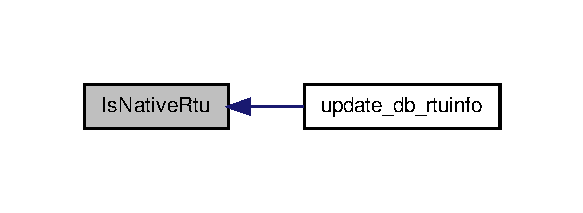
\includegraphics[width=280pt]{dbbase_8cpp_a55f5cb081a0fc3774070718f283746d6_icgraph}
\end{center}
\end{figure}


\hypertarget{dbbase_8cpp_ae130c9ff11734f9b283c749b1c682659}{\index{dbbase.\-cpp@{dbbase.\-cpp}!Is\-Safety\-Rtu@{Is\-Safety\-Rtu}}
\index{Is\-Safety\-Rtu@{Is\-Safety\-Rtu}!dbbase.cpp@{dbbase.\-cpp}}
\subsubsection[{Is\-Safety\-Rtu}]{\setlength{\rightskip}{0pt plus 5cm}bool Is\-Safety\-Rtu (
\begin{DoxyParamCaption}
\item[{{\bf Uint8}}]{type}
\end{DoxyParamCaption}
)}}\label{dbbase_8cpp_ae130c9ff11734f9b283c749b1c682659}


Is\-Safety\-Rtu 查看某设备是否是安防设备 


\begin{DoxyParams}{Parameters}
{\em type} & 设备类型\\
\hline
\end{DoxyParams}
\begin{DoxyReturn}{Returns}
true or false 
\end{DoxyReturn}


References R\-T\-U\-\_\-\-T\-Y\-P\-E\-\_\-\-D\-O\-O\-R\-B\-E\-L\-L, R\-T\-U\-\_\-\-T\-Y\-P\-E\-\_\-\-D\-O\-O\-R\-C\-O\-N\-T\-A\-C\-T, R\-T\-U\-\_\-\-T\-Y\-P\-E\-\_\-\-D\-O\-O\-R\-L\-O\-C\-K, and R\-T\-U\-\_\-\-T\-Y\-P\-E\-\_\-\-I\-R\-P\-R\-O\-B\-E.

\hypertarget{dbbase_8cpp_a334c4412fa09aab89d49cefdfd233b04}{\index{dbbase.\-cpp@{dbbase.\-cpp}!select\-\_\-db\-\_\-hostinfo@{select\-\_\-db\-\_\-hostinfo}}
\index{select\-\_\-db\-\_\-hostinfo@{select\-\_\-db\-\_\-hostinfo}!dbbase.cpp@{dbbase.\-cpp}}
\subsubsection[{select\-\_\-db\-\_\-hostinfo}]{\setlength{\rightskip}{0pt plus 5cm}int select\-\_\-db\-\_\-hostinfo (
\begin{DoxyParamCaption}
\item[{{\bf Host\-Reg\-Info} $\ast$}]{p\-Hostinfo, }
\item[{char $\ast$}]{hostname}
\end{DoxyParamCaption}
)}}\label{dbbase_8cpp_a334c4412fa09aab89d49cefdfd233b04}


select\-\_\-db\-\_\-hostinfo 根据主机名 查询主机信息 ,用于 A\-P\-P远程登陆 


\begin{DoxyParams}{Parameters}
{\em p\-Hostinfo} & \\
\hline
{\em hostname} & Host\-Add,Host\-Pwd,Host\-Ip,Host\-State,Last\-Com\-Time \\
\hline
\end{DoxyParams}
\begin{DoxyReturn}{Returns}
返回值 -\/1 错误 0 正确 1 没有数据 
\end{DoxyReturn}


References db\-\_\-select\-\_\-query(), D\-B\-\_\-\-T\-A\-B\-L\-E\-\_\-\-N\-A\-M\-E\-L\-I\-S\-T, Host\-Reg\-Info\-::hostadd, Host\-Reg\-Info\-::hostip, Host\-Reg\-Info\-::hostpwd, Host\-Reg\-Info\-::hoststate, Host\-Reg\-Info\-::lastcomtime, L\-O\-G\-\_\-\-D\-E\-B\-U\-G, and L\-O\-G\-\_\-\-E\-R\-R\-O\-R.



Here is the call graph for this function\-:\nopagebreak
\begin{figure}[H]
\begin{center}
\leavevmode
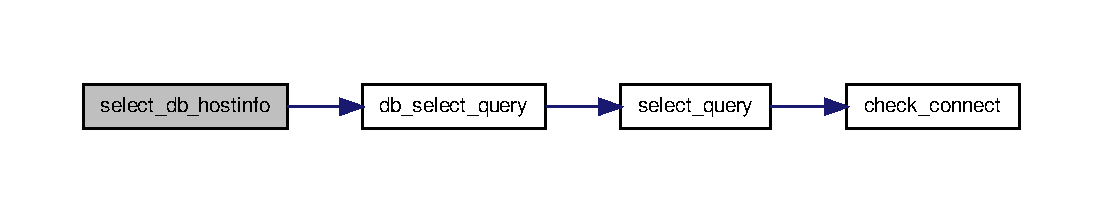
\includegraphics[width=350pt]{dbbase_8cpp_a334c4412fa09aab89d49cefdfd233b04_cgraph}
\end{center}
\end{figure}


\hypertarget{dbbase_8cpp_acdefe48f4a7a750062898c54c5ecd356}{\index{dbbase.\-cpp@{dbbase.\-cpp}!select\-\_\-query@{select\-\_\-query}}
\index{select\-\_\-query@{select\-\_\-query}!dbbase.cpp@{dbbase.\-cpp}}
\subsubsection[{select\-\_\-query}]{\setlength{\rightskip}{0pt plus 5cm}static int select\-\_\-query (
\begin{DoxyParamCaption}
\item[{const string \&}]{sql, }
\item[{string \&}]{retstr}
\end{DoxyParamCaption}
)\hspace{0.3cm}{\ttfamily [static]}}}\label{dbbase_8cpp_acdefe48f4a7a750062898c54c5ecd356}


select\-\_\-query 查找操作 


\begin{DoxyParams}{Parameters}
{\em sql} & 查找sql 命令 \\
\hline
{\em retstr} & 返回列字段,以逗号隔开\\
\hline
\end{DoxyParams}
\begin{DoxyReturn}{Returns}

\end{DoxyReturn}


References check\-\_\-connect(), L\-O\-G\-\_\-\-D\-E\-B\-U\-G, L\-O\-G\-\_\-\-E\-R\-R\-O\-R, and m\-\_\-mysqlfd.



Referenced by db\-\_\-select\-\_\-query().



Here is the call graph for this function\-:\nopagebreak
\begin{figure}[H]
\begin{center}
\leavevmode
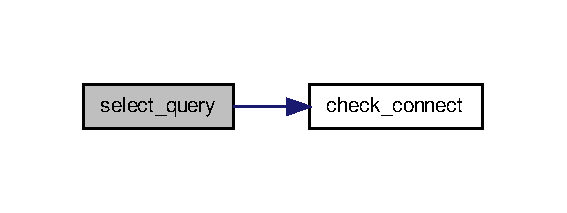
\includegraphics[width=272pt]{dbbase_8cpp_acdefe48f4a7a750062898c54c5ecd356_cgraph}
\end{center}
\end{figure}




Here is the caller graph for this function\-:\nopagebreak
\begin{figure}[H]
\begin{center}
\leavevmode
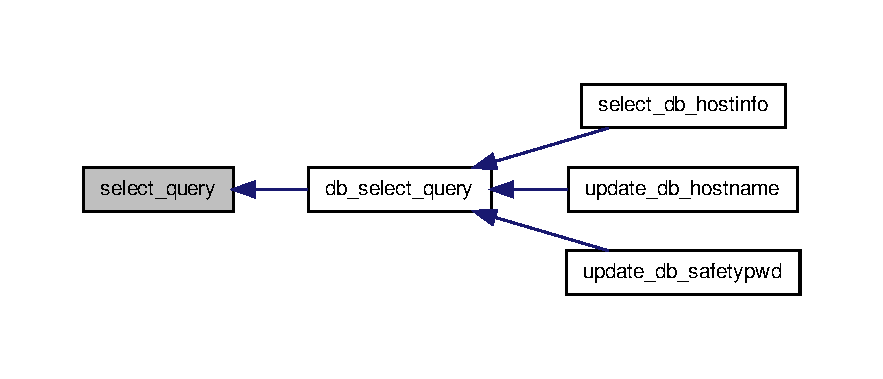
\includegraphics[width=350pt]{dbbase_8cpp_acdefe48f4a7a750062898c54c5ecd356_icgraph}
\end{center}
\end{figure}


\hypertarget{dbbase_8cpp_a8b214bd5c7dbfef30ac417954cb0c5e2}{\index{dbbase.\-cpp@{dbbase.\-cpp}!update\-\_\-db\-\_\-apprtu@{update\-\_\-db\-\_\-apprtu}}
\index{update\-\_\-db\-\_\-apprtu@{update\-\_\-db\-\_\-apprtu}!dbbase.cpp@{dbbase.\-cpp}}
\subsubsection[{update\-\_\-db\-\_\-apprtu}]{\setlength{\rightskip}{0pt plus 5cm}int update\-\_\-db\-\_\-apprtu (
\begin{DoxyParamCaption}
\item[{{\bf App\-Rtu\-Info} \&}]{rtuinfo}
\end{DoxyParamCaption}
)}}\label{dbbase_8cpp_a8b214bd5c7dbfef30ac417954cb0c5e2}


update\-\_\-db\-\_\-apprtu 修改应用设备 



References insert\-\_\-db\-\_\-apprtu().



Here is the call graph for this function\-:\nopagebreak
\begin{figure}[H]
\begin{center}
\leavevmode
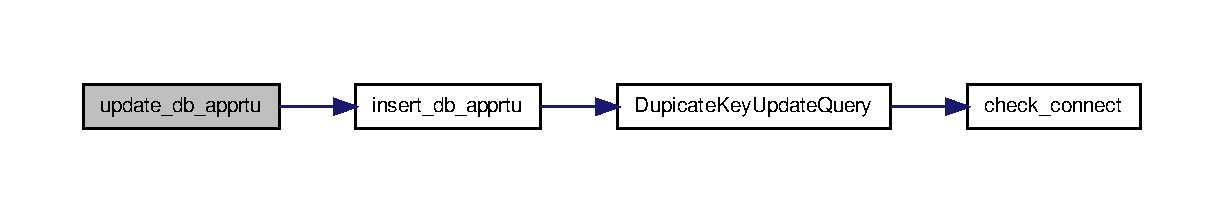
\includegraphics[width=350pt]{dbbase_8cpp_a8b214bd5c7dbfef30ac417954cb0c5e2_cgraph}
\end{center}
\end{figure}


\hypertarget{dbbase_8cpp_a35e1056e0f46576bda26dabc59ce0ded}{\index{dbbase.\-cpp@{dbbase.\-cpp}!update\-\_\-db\-\_\-detectorbind@{update\-\_\-db\-\_\-detectorbind}}
\index{update\-\_\-db\-\_\-detectorbind@{update\-\_\-db\-\_\-detectorbind}!dbbase.cpp@{dbbase.\-cpp}}
\subsubsection[{update\-\_\-db\-\_\-detectorbind}]{\setlength{\rightskip}{0pt plus 5cm}int update\-\_\-db\-\_\-detectorbind (
\begin{DoxyParamCaption}
\item[{{\bf Detector\-Bind} \&}]{rtuinfo}
\end{DoxyParamCaption}
)}}\label{dbbase_8cpp_a35e1056e0f46576bda26dabc59ce0ded}


update\-\_\-db\-\_\-detectorbind 绑定联动接口 


\begin{DoxyParams}{Parameters}
{\em rtuinfo} & 绑定的设备信息需要malloc后传入 \\
\hline
\end{DoxyParams}


References Rtu\-Bind\-::add, Detector\-Bind\-::bind\-\_\-num, db\-\_\-update\-\_\-query(), Rtu\-Bind\-::delay, Detector\-Bind\-::hostadd, Detector\-Bind\-::level, Rtu\-Bind\-::oper, Detector\-Bind\-::rtuadd, Detector\-Bind\-::rtubind, and Rtu\-Bind\-::type.



Here is the call graph for this function\-:\nopagebreak
\begin{figure}[H]
\begin{center}
\leavevmode
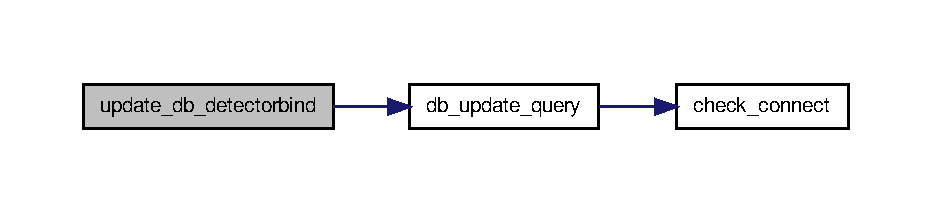
\includegraphics[width=350pt]{dbbase_8cpp_a35e1056e0f46576bda26dabc59ce0ded_cgraph}
\end{center}
\end{figure}


\hypertarget{dbbase_8cpp_aa039ebdc57c1a8157a01c9a762f43bc6}{\index{dbbase.\-cpp@{dbbase.\-cpp}!update\-\_\-db\-\_\-detectorrtu@{update\-\_\-db\-\_\-detectorrtu}}
\index{update\-\_\-db\-\_\-detectorrtu@{update\-\_\-db\-\_\-detectorrtu}!dbbase.cpp@{dbbase.\-cpp}}
\subsubsection[{update\-\_\-db\-\_\-detectorrtu}]{\setlength{\rightskip}{0pt plus 5cm}int update\-\_\-db\-\_\-detectorrtu (
\begin{DoxyParamCaption}
\item[{{\bf Detector\-Rtu} \&}]{rtuinfo, }
\item[{{\bf Uint8}}]{mode}
\end{DoxyParamCaption}
)}}\label{dbbase_8cpp_aa039ebdc57c1a8157a01c9a762f43bc6}


update\-\_\-db\-\_\-detectorrtu 更新传感器设备 


\begin{DoxyParams}{Parameters}
{\em rtuinfo} & \\
\hline
{\em mode} & 模式 0 更新 val 值 1 更新联动标志,阈值 更新val \-: 传入 val数组值 ,默认为0 更新联动标志: 传入 flag ,downval ,upval \\
\hline
\end{DoxyParams}
\begin{DoxyReturn}{Returns}

\end{DoxyReturn}


References db\-\_\-update\-\_\-query(), Detector\-Rtu\-::detectorinfo, Detector\-Info\-::downval, Detector\-Info\-::flag, Rtu\-Reg\-Info\-::hostadd, L\-O\-G\-\_\-\-E\-R\-R\-O\-R, Rtu\-Reg\-Info\-::rtuadd, Detector\-Rtu\-::rtuinfo, Detector\-Info\-::upval, Detector\-Info\-::val, and Detector\-Rtu\-::valtype.



Here is the call graph for this function\-:\nopagebreak
\begin{figure}[H]
\begin{center}
\leavevmode
\includegraphics[width=350pt]{dbbase_8cpp_aa039ebdc57c1a8157a01c9a762f43bc6_cgraph}
\end{center}
\end{figure}


\hypertarget{dbbase_8cpp_a81cfc05e7763f268740f8a27f85b77de}{\index{dbbase.\-cpp@{dbbase.\-cpp}!update\-\_\-db\-\_\-exnativertu@{update\-\_\-db\-\_\-exnativertu}}
\index{update\-\_\-db\-\_\-exnativertu@{update\-\_\-db\-\_\-exnativertu}!dbbase.cpp@{dbbase.\-cpp}}
\subsubsection[{update\-\_\-db\-\_\-exnativertu}]{\setlength{\rightskip}{0pt plus 5cm}int update\-\_\-db\-\_\-exnativertu (
\begin{DoxyParamCaption}
\item[{{\bf Ex\-Native\-Rtu} \&}]{rtuinfo}
\end{DoxyParamCaption}
)}}\label{dbbase_8cpp_a81cfc05e7763f268740f8a27f85b77de}


update\-\_\-db\-\_\-exnativertu 更新智能床 


\begin{DoxyParams}{Parameters}
{\em rtuinfo} & 控制 : relayinfo 数组 中val值传入 床头位置(1) 床尾位置(1) 床头振动(1) 床尾振动(1) 灯状态(1):0x00表示关灯,0x01表示开灯 \\
\hline
\end{DoxyParams}
\begin{DoxyReturn}{Returns}

\end{DoxyReturn}


References db\-\_\-update\-\_\-query(), get\-\_\-table\-\_\-name(), Rtu\-Reg\-Info\-::hostadd, Ex\-Native\-Rtu\-::relayinfo, R\-T\-U\-\_\-\-T\-Y\-P\-E\-\_\-\-B\-E\-D, Rtu\-Reg\-Info\-::rtuadd, Ex\-Native\-Rtu\-::rtuinfo, and Relay\-Info\-::val.



Here is the call graph for this function\-:\nopagebreak
\begin{figure}[H]
\begin{center}
\leavevmode
\includegraphics[width=350pt]{dbbase_8cpp_a81cfc05e7763f268740f8a27f85b77de_cgraph}
\end{center}
\end{figure}


\hypertarget{dbbase_8cpp_a82757fe4298d8fdf297391a4e42e3293}{\index{dbbase.\-cpp@{dbbase.\-cpp}!update\-\_\-db\-\_\-host@{update\-\_\-db\-\_\-host}}
\index{update\-\_\-db\-\_\-host@{update\-\_\-db\-\_\-host}!dbbase.cpp@{dbbase.\-cpp}}
\subsubsection[{update\-\_\-db\-\_\-host}]{\setlength{\rightskip}{0pt plus 5cm}int update\-\_\-db\-\_\-host (
\begin{DoxyParamCaption}
\item[{{\bf Host\-Reg\-Info} \&}]{hostinfo}
\end{DoxyParamCaption}
)}}\label{dbbase_8cpp_a82757fe4298d8fdf297391a4e42e3293}


update\-\_\-db\-\_\-host 更新主机信息表 


\begin{DoxyParams}{Parameters}
{\em hostinfo} & 更新信息: 传入 hostname ,hostip \\
\hline
\end{DoxyParams}
\begin{DoxyReturn}{Returns}

\end{DoxyReturn}


References db\-\_\-update\-\_\-query(), find\-Hostname(), get\-\_\-sys\-\_\-time(), get\-\_\-table\-\_\-name(), Host\-Reg\-Info\-::hostip, Host\-Reg\-Info\-::hostname, L\-O\-G\-\_\-\-E\-R\-R\-O\-R, and R\-T\-U\-\_\-\-T\-Y\-P\-E\-\_\-\-H\-O\-S\-T.



Here is the call graph for this function\-:\nopagebreak
\begin{figure}[H]
\begin{center}
\leavevmode
\includegraphics[width=350pt]{dbbase_8cpp_a82757fe4298d8fdf297391a4e42e3293_cgraph}
\end{center}
\end{figure}


\hypertarget{dbbase_8cpp_a5f38e8abcbb787b6fed1c8e1dce1c7c2}{\index{dbbase.\-cpp@{dbbase.\-cpp}!update\-\_\-db\-\_\-hostname@{update\-\_\-db\-\_\-hostname}}
\index{update\-\_\-db\-\_\-hostname@{update\-\_\-db\-\_\-hostname}!dbbase.cpp@{dbbase.\-cpp}}
\subsubsection[{update\-\_\-db\-\_\-hostname}]{\setlength{\rightskip}{0pt plus 5cm}int update\-\_\-db\-\_\-hostname (
\begin{DoxyParamCaption}
\item[{{\bf Host\-Man} \&}]{hostinfo}
\end{DoxyParamCaption}
)}}\label{dbbase_8cpp_a5f38e8abcbb787b6fed1c8e1dce1c7c2}


update\-\_\-db\-\_\-hostname 用户管理 


\begin{DoxyParams}{Parameters}
{\em hostinfo} & 更新信息: 传入 原 新 主机名 密码 \\
\hline
\end{DoxyParams}
\begin{DoxyReturn}{Returns}

\end{DoxyReturn}


References db\-\_\-select\-\_\-query(), db\-\_\-update\-\_\-query(), M\-A\-X\-\_\-\-P\-A\-S\-S\-W\-O\-R\-D\-\_\-\-L\-E\-N, Host\-Man\-::newname, Host\-Man\-::newpwd, Host\-Man\-::oldname, and Host\-Man\-::oldpwd.



Here is the call graph for this function\-:\nopagebreak
\begin{figure}[H]
\begin{center}
\leavevmode
\includegraphics[width=350pt]{dbbase_8cpp_a5f38e8abcbb787b6fed1c8e1dce1c7c2_cgraph}
\end{center}
\end{figure}


\hypertarget{dbbase_8cpp_a83758c046728190fe1ac0a9eef34285b}{\index{dbbase.\-cpp@{dbbase.\-cpp}!update\-\_\-db\-\_\-nativertu@{update\-\_\-db\-\_\-nativertu}}
\index{update\-\_\-db\-\_\-nativertu@{update\-\_\-db\-\_\-nativertu}!dbbase.cpp@{dbbase.\-cpp}}
\subsubsection[{update\-\_\-db\-\_\-nativertu}]{\setlength{\rightskip}{0pt plus 5cm}int update\-\_\-db\-\_\-nativertu (
\begin{DoxyParamCaption}
\item[{{\bf Native\-Rtu\-Info} \&}]{rtuinfo, }
\item[{{\bf Uint8}}]{mode}
\end{DoxyParamCaption}
)}}\label{dbbase_8cpp_a83758c046728190fe1ac0a9eef34285b}


update\-\_\-db\-\_\-nativertu 常规设备更新 


\begin{DoxyParams}{Parameters}
{\em rtuinfo} & \\
\hline
{\em mode} & 模式 0 控制 1 绑定负载 控制 : 传入 \hyperlink{structRelayInfo}{Relay\-Info} 数组中 val 绑定负载: 传入 bind\-\_\-num , \hyperlink{structRelayInfo}{Relay\-Info} 数组中 id,type,name\mbox{[}\mbox{]} ,path\mbox{[}\mbox{]} 设备头信息 \hyperlink{structRtuRegInfo}{Rtu\-Reg\-Info} 中的hostadd,rtuadd 必须传入 \\
\hline
\end{DoxyParams}
\begin{DoxyReturn}{Returns}
0 更新成功 -\/1 更新失败 
\end{DoxyReturn}


References Native\-Rtu\-Info\-::bind\-\_\-num, db\-\_\-update\-\_\-query(), Rtu\-Reg\-Info\-::hostadd, Relay\-Info\-::id, L\-O\-G\-\_\-\-D\-E\-B\-U\-G, L\-O\-G\-\_\-\-E\-R\-R\-O\-R, Relay\-Info\-::name, Relay\-Info\-::path, Native\-Rtu\-Info\-::relayinfo, Rtu\-Reg\-Info\-::rtuadd, Native\-Rtu\-Info\-::rtuinfo, Relay\-Info\-::type, and Relay\-Info\-::val.



Here is the call graph for this function\-:\nopagebreak
\begin{figure}[H]
\begin{center}
\leavevmode
\includegraphics[width=350pt]{dbbase_8cpp_a83758c046728190fe1ac0a9eef34285b_cgraph}
\end{center}
\end{figure}


\hypertarget{dbbase_8cpp_ad42e211ca6c04241e68331f73c74113c}{\index{dbbase.\-cpp@{dbbase.\-cpp}!update\-\_\-db\-\_\-rtuinfo@{update\-\_\-db\-\_\-rtuinfo}}
\index{update\-\_\-db\-\_\-rtuinfo@{update\-\_\-db\-\_\-rtuinfo}!dbbase.cpp@{dbbase.\-cpp}}
\subsubsection[{update\-\_\-db\-\_\-rtuinfo}]{\setlength{\rightskip}{0pt plus 5cm}int update\-\_\-db\-\_\-rtuinfo (
\begin{DoxyParamCaption}
\item[{{\bf Rtu\-Update} \&}]{hostinfo}
\end{DoxyParamCaption}
)}}\label{dbbase_8cpp_ad42e211ca6c04241e68331f73c74113c}


update\-\_\-db\-\_\-rtuinfo 用户设备信息编辑 


\begin{DoxyParams}{Parameters}
{\em hostinfo} & 该结构体所有字段必须传入 更新 设备名称和路径 \\
\hline
\end{DoxyParams}
\begin{DoxyReturn}{Returns}

\end{DoxyReturn}


References db\-\_\-update\-\_\-query(), get\-\_\-table\-\_\-name(), Rtu\-Update\-::hostadd, Is\-Native\-Rtu(), Rtu\-Update\-::opertype, R\-T\-U\-\_\-\-T\-Y\-P\-E\-\_\-\-B\-E\-D, R\-T\-U\-\_\-\-T\-Y\-P\-E\-\_\-\-S\-C\-E\-N\-E\-I\-N\-F\-O, R\-T\-U\-\_\-\-T\-Y\-P\-E\-\_\-\-T\-A\-S\-K\-I\-N\-F\-O, Rtu\-Update\-::rtuadd, Rtu\-Update\-::rtuname, Rtu\-Update\-::rtupath, and Rtu\-Update\-::rtutype.



Here is the call graph for this function\-:\nopagebreak
\begin{figure}[H]
\begin{center}
\leavevmode
\includegraphics[width=350pt]{dbbase_8cpp_ad42e211ca6c04241e68331f73c74113c_cgraph}
\end{center}
\end{figure}


\hypertarget{dbbase_8cpp_afe8cc79a0b360aa2a371f266709451e8}{\index{dbbase.\-cpp@{dbbase.\-cpp}!update\-\_\-db\-\_\-safetypwd@{update\-\_\-db\-\_\-safetypwd}}
\index{update\-\_\-db\-\_\-safetypwd@{update\-\_\-db\-\_\-safetypwd}!dbbase.cpp@{dbbase.\-cpp}}
\subsubsection[{update\-\_\-db\-\_\-safetypwd}]{\setlength{\rightskip}{0pt plus 5cm}int update\-\_\-db\-\_\-safetypwd (
\begin{DoxyParamCaption}
\item[{{\bf Safety\-Pwd\-Info} \&}]{rtuinfo}
\end{DoxyParamCaption}
)}}\label{dbbase_8cpp_afe8cc79a0b360aa2a371f266709451e8}


update\-\_\-db\-\_\-safetypwd 门锁密码更新接口 包括新开锁密码添加,修改 管理员密码修改 



References db\-\_\-select\-\_\-query(), db\-\_\-update\-\_\-query(), Safety\-Pwd\-Info\-::hostadd, Safety\-Pwd\-Info\-::id, L\-O\-G\-\_\-\-E\-R\-R\-O\-R, M\-A\-X\-\_\-\-P\-A\-S\-S\-W\-O\-R\-D\-\_\-\-L\-E\-N, Safety\-Pwd\-Info\-::newpwd, Safety\-Pwd\-Info\-::oldpwd, and Safety\-Pwd\-Info\-::rtuadd.



Here is the call graph for this function\-:\nopagebreak
\begin{figure}[H]
\begin{center}
\leavevmode
\includegraphics[width=350pt]{dbbase_8cpp_afe8cc79a0b360aa2a371f266709451e8_cgraph}
\end{center}
\end{figure}


\hypertarget{dbbase_8cpp_ae0e36aa1334e0b83d2e2edd95a89b5b2}{\index{dbbase.\-cpp@{dbbase.\-cpp}!update\-\_\-db\-\_\-safetyrtu@{update\-\_\-db\-\_\-safetyrtu}}
\index{update\-\_\-db\-\_\-safetyrtu@{update\-\_\-db\-\_\-safetyrtu}!dbbase.cpp@{dbbase.\-cpp}}
\subsubsection[{update\-\_\-db\-\_\-safetyrtu}]{\setlength{\rightskip}{0pt plus 5cm}int update\-\_\-db\-\_\-safetyrtu (
\begin{DoxyParamCaption}
\item[{{\bf Safety\-Rtu} \&}]{rtuinfo}
\end{DoxyParamCaption}
)}}\label{dbbase_8cpp_ae0e36aa1334e0b83d2e2edd95a89b5b2}


update\-\_\-db\-\_\-safetyrtu 更新安防设备 


\begin{DoxyParams}{Parameters}
{\em rtuinfo} & 控制: 传入 布防状态 , 动作状态 hostadd ,rtuadd 必须 传入 \\
\hline
\end{DoxyParams}
\begin{DoxyReturn}{Returns}

\end{DoxyReturn}


References db\-\_\-update\-\_\-query(), get\-\_\-table\-\_\-name(), Rtu\-Reg\-Info\-::hostadd, Safety\-Rtu\-::rtuactstate, Rtu\-Reg\-Info\-::rtuadd, Safety\-Rtu\-::rtuinfo, Safety\-Rtu\-::rtuplace, and Rtu\-Reg\-Info\-::rtutype.



Here is the call graph for this function\-:\nopagebreak
\begin{figure}[H]
\begin{center}
\leavevmode
\includegraphics[width=350pt]{dbbase_8cpp_ae0e36aa1334e0b83d2e2edd95a89b5b2_cgraph}
\end{center}
\end{figure}


\hypertarget{dbbase_8cpp_aedbae4394a0f4e1fc8f6eabee7e355c2}{\index{dbbase.\-cpp@{dbbase.\-cpp}!update\-\_\-db\-\_\-sceneinfo@{update\-\_\-db\-\_\-sceneinfo}}
\index{update\-\_\-db\-\_\-sceneinfo@{update\-\_\-db\-\_\-sceneinfo}!dbbase.cpp@{dbbase.\-cpp}}
\subsubsection[{update\-\_\-db\-\_\-sceneinfo}]{\setlength{\rightskip}{0pt plus 5cm}int update\-\_\-db\-\_\-sceneinfo (
\begin{DoxyParamCaption}
\item[{{\bf Scene\-Info} \&}]{rtuinfo}
\end{DoxyParamCaption}
)}}\label{dbbase_8cpp_aedbae4394a0f4e1fc8f6eabee7e355c2}


update\-\_\-db\-\_\-sceneinfo 修改 情景 



References insert\-\_\-db\-\_\-sceneinfo().



Referenced by main().



Here is the call graph for this function\-:\nopagebreak
\begin{figure}[H]
\begin{center}
\leavevmode
\includegraphics[width=350pt]{dbbase_8cpp_aedbae4394a0f4e1fc8f6eabee7e355c2_cgraph}
\end{center}
\end{figure}




Here is the caller graph for this function\-:\nopagebreak
\begin{figure}[H]
\begin{center}
\leavevmode
\includegraphics[width=264pt]{dbbase_8cpp_aedbae4394a0f4e1fc8f6eabee7e355c2_icgraph}
\end{center}
\end{figure}


\hypertarget{dbbase_8cpp_aae594d8934a37c3a973e31432cd76c96}{\index{dbbase.\-cpp@{dbbase.\-cpp}!update\-\_\-db\-\_\-scenertu@{update\-\_\-db\-\_\-scenertu}}
\index{update\-\_\-db\-\_\-scenertu@{update\-\_\-db\-\_\-scenertu}!dbbase.cpp@{dbbase.\-cpp}}
\subsubsection[{update\-\_\-db\-\_\-scenertu}]{\setlength{\rightskip}{0pt plus 5cm}int update\-\_\-db\-\_\-scenertu (
\begin{DoxyParamCaption}
\item[{{\bf Scene\-Rtu} \&}]{rtuinfo}
\end{DoxyParamCaption}
)}}\label{dbbase_8cpp_aae594d8934a37c3a973e31432cd76c96}


update\-\_\-db\-\_\-scenertu 更新情景面板 


\begin{DoxyParams}{Parameters}
{\em rtuinfo} & 修改绑定: bind\-\_\-num , 每个button的信息 ,包括id ,type,add,oper \\
\hline
\end{DoxyParams}
\begin{DoxyReturn}{Returns}

\end{DoxyReturn}


References Scene\-Bind\-::add, Scene\-Rtu\-::bind\-\_\-num, db\-\_\-update\-\_\-query(), Rtu\-Reg\-Info\-::hostadd, Scene\-Bind\-::id, Scene\-Bind\-::oper, Rtu\-Reg\-Info\-::rtuadd, Scene\-Rtu\-::rtuinfo, Scene\-Rtu\-::scene\-\_\-bind, and Scene\-Bind\-::type.



Here is the call graph for this function\-:\nopagebreak
\begin{figure}[H]
\begin{center}
\leavevmode
\includegraphics[width=350pt]{dbbase_8cpp_aae594d8934a37c3a973e31432cd76c96_cgraph}
\end{center}
\end{figure}


\hypertarget{dbbase_8cpp_a659d4acf9f3d7a1b013867717905c198}{\index{dbbase.\-cpp@{dbbase.\-cpp}!update\-\_\-db\-\_\-taskinfo@{update\-\_\-db\-\_\-taskinfo}}
\index{update\-\_\-db\-\_\-taskinfo@{update\-\_\-db\-\_\-taskinfo}!dbbase.cpp@{dbbase.\-cpp}}
\subsubsection[{update\-\_\-db\-\_\-taskinfo}]{\setlength{\rightskip}{0pt plus 5cm}int update\-\_\-db\-\_\-taskinfo (
\begin{DoxyParamCaption}
\item[{{\bf Task\-Info} \&}]{taskinfo}
\end{DoxyParamCaption}
)}}\label{dbbase_8cpp_a659d4acf9f3d7a1b013867717905c198}


update\-\_\-db\-\_\-taskinfo 编辑定时任务 



References insert\-\_\-db\-\_\-taskinfo().



Referenced by main().



Here is the call graph for this function\-:\nopagebreak
\begin{figure}[H]
\begin{center}
\leavevmode
\includegraphics[width=350pt]{dbbase_8cpp_a659d4acf9f3d7a1b013867717905c198_cgraph}
\end{center}
\end{figure}




Here is the caller graph for this function\-:\nopagebreak
\begin{figure}[H]
\begin{center}
\leavevmode
\includegraphics[width=256pt]{dbbase_8cpp_a659d4acf9f3d7a1b013867717905c198_icgraph}
\end{center}
\end{figure}




\subsection{Variable Documentation}
\hypertarget{dbbase_8cpp_a513b454acfc51fb3100e5a8ad0535b50}{\index{dbbase.\-cpp@{dbbase.\-cpp}!m\-\_\-mysqlfd@{m\-\_\-mysqlfd}}
\index{m\-\_\-mysqlfd@{m\-\_\-mysqlfd}!dbbase.cpp@{dbbase.\-cpp}}
\subsubsection[{m\-\_\-mysqlfd}]{\setlength{\rightskip}{0pt plus 5cm}M\-Y\-S\-Q\-L m\-\_\-mysqlfd}}\label{dbbase_8cpp_a513b454acfc51fb3100e5a8ad0535b50}
数据库连接描述符 

Referenced by check\-\_\-connect(), db\-\_\-update\-\_\-query(), delete\-\_\-db\-\_\-host(), delete\-\_\-db\-\_\-rtu(), Dupicate\-Key\-Update\-Query(), find\-Hostname(), find\-Rtuadd(), Get\-Host\-Count(), Get\-Host\-Id\-By\-Name(), Get\-Ip\-By\-Host\-Add(), init\-\_\-mysql(), insert\-\_\-db\-\_\-rtu(), insert\-\_\-mysql(), and select\-\_\-query().


\hypertarget{dbbase_8h}{\section{dbbase.\-h File Reference}
\label{dbbase_8h}\index{dbbase.\-h@{dbbase.\-h}}
}


mysql 数据库接口实现  


{\ttfamily \#include $<$stdio.\-h$>$}\\*
{\ttfamily \#include $<$mysql/mysql.\-h$>$}\\*
{\ttfamily \#include $<$sstream$>$}\\*
{\ttfamily \#include $<$iostream$>$}\\*
{\ttfamily \#include $<$string.\-h$>$}\\*
{\ttfamily \#include \char`\"{}base.\-h\char`\"{}}\\*
Include dependency graph for dbbase.\-h\-:\nopagebreak
\begin{figure}[H]
\begin{center}
\leavevmode
\includegraphics[width=350pt]{dbbase_8h__incl}
\end{center}
\end{figure}
This graph shows which files directly or indirectly include this file\-:\nopagebreak
\begin{figure}[H]
\begin{center}
\leavevmode
\includegraphics[width=212pt]{dbbase_8h__dep__incl}
\end{center}
\end{figure}
\subsection*{Data Structures}
\begin{DoxyCompactItemize}
\item 
struct \hyperlink{structDBTypeInfo}{D\-B\-Type\-Info}
\item 
struct \hyperlink{structMysqlConInfo}{Mysql\-Con\-Info}
\item 
struct \hyperlink{structRtuRegInfo}{Rtu\-Reg\-Info}
\item 
struct \hyperlink{structRtuRemoveInfo}{Rtu\-Remove\-Info}
\item 
struct \hyperlink{structHostRegInfo}{Host\-Reg\-Info}
\item 
struct \hyperlink{structAppRtuInfo}{App\-Rtu\-Info}
\item 
struct \hyperlink{structRelayInfo}{Relay\-Info}
\item 
struct \hyperlink{structNativeRtuInfo}{Native\-Rtu\-Info}
\item 
struct \hyperlink{structSafetyRtu}{Safety\-Rtu}
\item 
struct \hyperlink{structSceneBind}{Scene\-Bind}
\item 
struct \hyperlink{structSceneRtu}{Scene\-Rtu}
\item 
struct \hyperlink{structExNativeRtu}{Ex\-Native\-Rtu}
\item 
struct \hyperlink{structDetectorInfo}{Detector\-Info}
\item 
struct \hyperlink{structDetectorRtu}{Detector\-Rtu}
\item 
struct \hyperlink{structRtuBind}{Rtu\-Bind}
\item 
struct \hyperlink{structDetectorBind}{Detector\-Bind}
\item 
struct \hyperlink{structTaskInfo}{Task\-Info}
\item 
struct \hyperlink{structSceneInfo}{Scene\-Info}
\item 
struct \hyperlink{structHostMan}{Host\-Man}
\item 
struct \hyperlink{structRtuUpdate}{Rtu\-Update}
\item 
struct \hyperlink{structSafetyPwdInfo}{Safety\-Pwd\-Info}
\end{DoxyCompactItemize}
\subsection*{Macros}
\begin{DoxyCompactItemize}
\item 
\#define \hyperlink{dbbase_8h_a06a9cf374e83dcac0620e5095f79234e}{M\-A\-X\-\_\-\-S\-Q\-L\-N\-A\-M\-E\-\_\-\-L\-E\-N}~256
\begin{DoxyCompactList}\small\item\em 数据库主机长度 \end{DoxyCompactList}\item 
\#define \hyperlink{dbbase_8h_a6c4647395896246d6710ba980c31666c}{M\-A\-X\-\_\-\-U\-S\-E\-R\-N\-A\-M\-E\-\_\-\-L\-E\-N}~32
\begin{DoxyCompactList}\small\item\em 用户名长度 \end{DoxyCompactList}\item 
\#define \hyperlink{dbbase_8h_ae9169c3fda2dfecbb7a13e394a69e5be}{M\-A\-X\-\_\-\-P\-A\-S\-S\-W\-O\-R\-D\-\_\-\-L\-E\-N}~16
\begin{DoxyCompactList}\small\item\em 用户密码长度 \end{DoxyCompactList}\item 
\#define \hyperlink{dbbase_8h_a998c6ce37817a02bf23a1a2c6fd15cb0}{M\-A\-X\-\_\-\-S\-Q\-L\-U\-S\-E\-R\-N\-A\-M\-E\-\_\-\-L\-E\-N}~16
\begin{DoxyCompactList}\small\item\em 数据库用户名长度 \end{DoxyCompactList}\item 
\#define \hyperlink{dbbase_8h_ae5cf418bda87e648ae461cfbca7e2f8e}{M\-A\-X\-\_\-\-S\-Q\-L\-P\-A\-S\-S\-W\-D\-\_\-\-L\-E\-N}~32
\begin{DoxyCompactList}\small\item\em 数据库密码 \end{DoxyCompactList}\item 
\#define \hyperlink{dbbase_8h_a7a31b64ea7a37ca824e574b1ac483c4e}{M\-I\-N\-\_\-\-P\-A\-T\-H\-\_\-\-L\-E\-N}~32
\begin{DoxyCompactList}\small\item\em 最小路径名长度 \end{DoxyCompactList}\item 
\#define \hyperlink{dbbase_8h_afd709f201d7643c3909621f620ea648a}{M\-A\-X\-\_\-\-N\-A\-M\-E\-\_\-\-L\-E\-N}~32
\begin{DoxyCompactList}\small\item\em 最大名称描述长度 \end{DoxyCompactList}\item 
\#define \hyperlink{dbbase_8h_a996a9eb45ccaa6031bb6c2756982574e}{D\-B\-\_\-\-T\-Y\-P\-E\-\_\-\-H\-O\-S\-T\-I\-N\-F\-O}~0
\begin{DoxyCompactList}\small\item\em 主机信息 \end{DoxyCompactList}\item 
\#define \hyperlink{dbbase_8h_a41cec6fbd71ae961f90e82426069de0d}{D\-B\-\_\-\-T\-Y\-P\-E\-\_\-\-N\-A\-T\-I\-V\-E\-R\-T\-U}~1
\begin{DoxyCompactList}\small\item\em 常规设备数据对象类型,即对应设备类型中的智能开关、智能插座、继电器控制盒、\-R\-G\-B灯、窗帘控制器 \end{DoxyCompactList}\item 
\#define \hyperlink{dbbase_8h_ad4f12324caffd9b4f08873fab1e000ec}{D\-B\-\_\-\-T\-Y\-P\-E\-\_\-\-S\-C\-E\-N\-E\-R\-T\-U}~2
\begin{DoxyCompactList}\small\item\em 情景面板数据对象类型,即对应设备类型中的情景面板 \end{DoxyCompactList}\item 
\#define \hyperlink{dbbase_8h_a41a148f7a529e4db02e65558c4e8bd2a}{D\-B\-\_\-\-T\-Y\-P\-E\-\_\-\-S\-C\-E\-N\-E\-I\-N\-F\-O}~3
\begin{DoxyCompactList}\small\item\em 情景信息数据对象类型,与设备类型无关 \end{DoxyCompactList}\item 
\#define \hyperlink{dbbase_8h_a7eb9f10805359d86e3bc2f3db4f637a0}{D\-B\-\_\-\-T\-Y\-P\-E\-\_\-\-T\-R\-A\-N\-S\-P\-O\-N\-D}~4
\begin{DoxyCompactList}\small\item\em 转发设备数据对象类型,即对应设备类型中的蓝牙遥控器、红外转发器 \end{DoxyCompactList}\item 
\#define \hyperlink{dbbase_8h_ae55710d69649f16efe243531ff2a81bf}{D\-B\-\_\-\-T\-Y\-P\-E\-\_\-\-U\-S\-E\-D\-E\-V\-I\-C\-E}~5
\begin{DoxyCompactList}\small\item\em 应用设备对象类型,即对应设备类型中的应用设备 \end{DoxyCompactList}\item 
\#define \hyperlink{dbbase_8h_aa5fd110ec2d2154dd1551fd95e067656}{D\-B\-\_\-\-T\-Y\-P\-E\-\_\-\-S\-A\-F\-E\-T\-Y}~6
\begin{DoxyCompactList}\small\item\em 安防设备数据对象类型,即对应设备类型中的红外入侵探测器、智能门磁、智能门锁、智能门铃 \end{DoxyCompactList}\item 
\#define \hyperlink{dbbase_8h_a61d59a6754031f39ebda58da8b952ba1}{D\-B\-\_\-\-T\-Y\-P\-E\-\_\-\-S\-A\-F\-E\-T\-Y\-\_\-\-P\-W\-D}~7
\begin{DoxyCompactList}\small\item\em 安防设备数据的密码 \end{DoxyCompactList}\item 
\#define \hyperlink{dbbase_8h_aec430d5db9094084b6e15d22ed4819a5}{D\-B\-\_\-\-T\-Y\-P\-E\-\_\-\-S\-A\-F\-E\-T\-Y\-\_\-\-S\-E\-T}~8
\begin{DoxyCompactList}\small\item\em 安防设备数据的设防联动 \end{DoxyCompactList}\item 
\#define \hyperlink{dbbase_8h_a5e6cbdcc4f0d7de1fea79c99558b360f}{D\-B\-\_\-\-T\-Y\-P\-E\-\_\-\-S\-A\-F\-E\-T\-Y\-\_\-\-R\-E\-M\-O\-V\-E}~9
\begin{DoxyCompactList}\small\item\em 安防设备数据的撤防联动 \end{DoxyCompactList}\item 
\#define \hyperlink{dbbase_8h_a5f8a196b1bd807b23e6f2cfd4e19de85}{D\-B\-\_\-\-T\-Y\-P\-E\-\_\-\-S\-C\-E\-N\-E\-I\-N\-F\-O\-\_\-\-C\-O\-N}~10
\begin{DoxyCompactList}\small\item\em 情景信息续表 \end{DoxyCompactList}\item 
\#define \hyperlink{dbbase_8h_a3fb36a0a73a2cfe354d3b92d685486fb}{D\-B\-\_\-\-T\-Y\-P\-E\-\_\-\-D\-E\-T\-E\-C\-T\-O\-R\-R\-T\-U}~11
\begin{DoxyCompactList}\small\item\em 传感器设备数据对象类型 \end{DoxyCompactList}\item 
\#define \hyperlink{dbbase_8h_a916a559281a114bcb4d1eab8037e3b83}{D\-B\-\_\-\-T\-Y\-P\-E\-\_\-\-D\-E\-T\-E\-C\-T\-O\-R\-B\-I\-N\-D}~12
\begin{DoxyCompactList}\small\item\em 传感器设备联动 \end{DoxyCompactList}\item 
\#define \hyperlink{dbbase_8h_aed911e3974cf3a23a323d798cdc50621}{D\-B\-\_\-\-T\-Y\-P\-E\-\_\-\-T\-A\-S\-K\-I\-N\-F\-O}~13
\item 
\#define \hyperlink{dbbase_8h_a2bd6cf12d4f631f21eea2b7fe1a59394}{D\-B\-\_\-\-T\-Y\-P\-E\-\_\-\-E\-X\-N\-A\-T\-I\-V\-E\-R\-T\-U}~14
\item 
\#define \hyperlink{dbbase_8h_a76dca32c9108e44ce73937259d5e7dee}{M\-A\-X\-\_\-\-D\-B\-\_\-\-T\-Y\-P\-E}~15
\item 
\#define \hyperlink{dbbase_8h_a9ab465f58189825ead59fe8a79c2a7f6}{D\-B\-\_\-\-T\-Y\-P\-E\-\_\-\-R\-T\-U\-T\-Y\-P\-E}~(\hyperlink{dbbase_8h_a76dca32c9108e44ce73937259d5e7dee}{M\-A\-X\-\_\-\-D\-B\-\_\-\-T\-Y\-P\-E})
\item 
\#define \hyperlink{dbbase_8h_abe648858953c8e5a22b1cd5802ce6b0f}{D\-B\-\_\-\-T\-Y\-P\-E\-\_\-\-U\-S\-E\-D\-E\-V\-T\-Y\-P\-E}~(\hyperlink{dbbase_8h_a76dca32c9108e44ce73937259d5e7dee}{M\-A\-X\-\_\-\-D\-B\-\_\-\-T\-Y\-P\-E}+1)
\item 
\#define \hyperlink{dbbase_8h_a95e59c426d2f33d0653e61e86998c1a1}{R\-T\-U\-\_\-\-T\-Y\-P\-E\-\_\-\-H\-O\-S\-T}~0
\begin{DoxyCompactList}\small\item\em 主机类型 \end{DoxyCompactList}\item 
\#define \hyperlink{dbbase_8h_aed90f514e1e21d48002da1e555617aab}{R\-T\-U\-\_\-\-T\-Y\-P\-E\-\_\-\-S\-W\-I\-T\-C\-H}~1
\begin{DoxyCompactList}\small\item\em 智能开关类型 \end{DoxyCompactList}\item 
\#define \hyperlink{dbbase_8h_aad9835fec88827746383cbfc49d11d98}{R\-T\-U\-\_\-\-T\-Y\-P\-E\-\_\-\-S\-C\-E\-N\-E}~2
\begin{DoxyCompactList}\small\item\em 情景面板类型 \end{DoxyCompactList}\item 
\#define \hyperlink{dbbase_8h_a4dd9a3011fd8aedf02308903c9129cc7}{R\-T\-U\-\_\-\-T\-Y\-P\-E\-\_\-\-P\-L\-U\-G}~3
\begin{DoxyCompactList}\small\item\em 智能插座类型 \end{DoxyCompactList}\item 
\#define \hyperlink{dbbase_8h_aaa53b0895b2ab0fcf07391ac59c2a775}{R\-T\-U\-\_\-\-T\-Y\-P\-E\-\_\-\-C\-T\-R\-L\-B\-O\-X}~4
\begin{DoxyCompactList}\small\item\em 继电器控制盒类型 \end{DoxyCompactList}\item 
\#define \hyperlink{dbbase_8h_afa871f118a4976960003db5923b783b3}{R\-T\-U\-\_\-\-T\-Y\-P\-E\-\_\-\-R\-G\-B}~5
\begin{DoxyCompactList}\small\item\em R\-G\-B灯 \end{DoxyCompactList}\item 
\#define \hyperlink{dbbase_8h_a1a0d47652142cbb9c1bcb0cf80b47d92}{R\-T\-U\-\_\-\-T\-Y\-P\-E\-\_\-\-B\-T\-R\-E\-M\-O\-T\-E}~6
\begin{DoxyCompactList}\small\item\em 蓝牙遥控器 \end{DoxyCompactList}\item 
\#define \hyperlink{dbbase_8h_afdf7c2bf60db37561d4f8a78b75f849c}{R\-T\-U\-\_\-\-T\-Y\-P\-E\-\_\-\-I\-R\-T\-R\-A\-N\-S}~7
\begin{DoxyCompactList}\small\item\em 红外转发器 \end{DoxyCompactList}\item 
\#define \hyperlink{dbbase_8h_a9570babe61ff0e57b4599cb5b73c48fb}{R\-T\-U\-\_\-\-T\-Y\-P\-E\-\_\-\-C\-U\-R\-T\-A\-I\-N}~8
\begin{DoxyCompactList}\small\item\em 窗帘控制器 \end{DoxyCompactList}\item 
\#define \hyperlink{dbbase_8h_ad4d8ed4e32dd5fb1c51c108cca3a8554}{R\-T\-U\-\_\-\-T\-Y\-P\-E\-\_\-\-I\-R\-P\-R\-O\-B\-E}~9
\begin{DoxyCompactList}\small\item\em 红外入侵探测器 \end{DoxyCompactList}\item 
\#define \hyperlink{dbbase_8h_ac058536e995f3b3bee62f55f09b1c173}{R\-T\-U\-\_\-\-T\-Y\-P\-E\-\_\-\-D\-O\-O\-R\-C\-O\-N\-T\-A\-C\-T}~10
\begin{DoxyCompactList}\small\item\em 智能门磁 \end{DoxyCompactList}\item 
\#define \hyperlink{dbbase_8h_a2509d905cb6eac619dceb509307e73fe}{R\-T\-U\-\_\-\-T\-Y\-P\-E\-\_\-\-D\-O\-O\-R\-L\-O\-C\-K}~11
\begin{DoxyCompactList}\small\item\em 智能门锁 \end{DoxyCompactList}\item 
\#define \hyperlink{dbbase_8h_a7bd5a16f13b698e65ddb74512dbe3a66}{R\-T\-U\-\_\-\-T\-Y\-P\-E\-\_\-\-D\-O\-O\-R\-B\-E\-L\-L}~12
\begin{DoxyCompactList}\small\item\em 智能门铃 \end{DoxyCompactList}\item 
\#define \hyperlink{dbbase_8h_ad962222c561832b09a2ce2740238b4c4}{R\-T\-U\-\_\-\-T\-Y\-P\-E\-\_\-\-L\-I\-G\-H\-T\-D\-E\-T}~13
\begin{DoxyCompactList}\small\item\em 光照探测器 \end{DoxyCompactList}\item 
\#define \hyperlink{dbbase_8h_aabeed00c2ac99b59fd1cd6339863838f}{R\-T\-U\-\_\-\-T\-Y\-P\-E\-\_\-\-G\-A\-S\-D\-E\-T}~14
\begin{DoxyCompactList}\small\item\em 可燃气探测器 \end{DoxyCompactList}\item 
\#define \hyperlink{dbbase_8h_a93c307e01bad7e244af2477a33910ebc}{R\-T\-U\-\_\-\-T\-Y\-P\-E\-\_\-\-T\-P\-M\-H\-U\-M\-D\-E\-T}~15
\begin{DoxyCompactList}\small\item\em 温湿度空气质量探测器 \end{DoxyCompactList}\item 
\#define \hyperlink{dbbase_8h_a856db09b936bf3fac6b6076f4fe9e6c1}{R\-T\-U\-\_\-\-T\-Y\-P\-E\-\_\-\-D\-A\-M\-D\-E\-T}~16
\begin{DoxyCompactList}\small\item\em 湿敏探测器 \end{DoxyCompactList}\item 
\#define \hyperlink{dbbase_8h_ab9e97b016d165c0848d9e26dbb732bb5}{R\-T\-U\-\_\-\-T\-Y\-P\-E\-\_\-\-R\-O\-B\-T\-I\-C}~17
\begin{DoxyCompactList}\small\item\em 机械手 \end{DoxyCompactList}\item 
\#define \hyperlink{dbbase_8h_af2fd88a1eb8ff4c2bffbb73639b393d5}{R\-T\-U\-\_\-\-T\-Y\-P\-E\-\_\-\-B\-E\-D}~18
\begin{DoxyCompactList}\small\item\em 智能床 \end{DoxyCompactList}\item 
\#define \hyperlink{dbbase_8h_aceaf727eed5d28b335b91a7474e976ae}{R\-T\-U\-\_\-\-T\-Y\-P\-E\-\_\-\-U\-S\-E\-R\-I\-N\-F\-O}~0xf8
\begin{DoxyCompactList}\small\item\em 用户信息 \end{DoxyCompactList}\item 
\#define \hyperlink{dbbase_8h_abe151b74d26cdd9dd31923846454c9d0}{R\-T\-U\-\_\-\-T\-Y\-P\-E\-\_\-\-F\-L\-O\-O\-R\-I\-N\-F\-O}~0xf9
\begin{DoxyCompactList}\small\item\em 楼层信息 \end{DoxyCompactList}\item 
\#define \hyperlink{dbbase_8h_ac5684c1ee2f398b9f88b89cfcf746eca}{R\-T\-U\-\_\-\-T\-Y\-P\-E\-\_\-\-U\-S\-E\-D\-E\-V\-I\-C\-E}~0xfa
\begin{DoxyCompactList}\small\item\em 应用设备,如用户的电视、空调、机机盒、摄像头 \end{DoxyCompactList}\item 
\#define \hyperlink{dbbase_8h_ad45e0faaa50bbd77ad0f3ef05b8b8c5d}{R\-T\-U\-\_\-\-T\-Y\-P\-E\-\_\-\-S\-E\-R\-V\-E\-R}~0xfb
\item 
\#define \hyperlink{dbbase_8h_acd85ffd783088af534e8a3f285f1a787}{R\-T\-U\-\_\-\-T\-Y\-P\-E\-\_\-\-T\-A\-S\-K\-I\-N\-F\-O}~0xfc
\begin{DoxyCompactList}\small\item\em 任务信息,即存储的数据 \end{DoxyCompactList}\item 
\#define \hyperlink{dbbase_8h_a5b85ab36fa49bdaa0e0aba8ef2c49e81}{R\-T\-U\-\_\-\-T\-Y\-P\-E\-\_\-\-S\-C\-E\-N\-E\-I\-N\-F\-O}~0xfd
\begin{DoxyCompactList}\small\item\em 情景信息,即存储的数据 \end{DoxyCompactList}\item 
\#define \hyperlink{dbbase_8h_a7f4cd829adead6136dfbffd8d3beb9ca}{R\-T\-U\-\_\-\-T\-Y\-P\-E\-\_\-\-A\-P\-P}~0xfe
\begin{DoxyCompactList}\small\item\em A\-P\-P应用程序 \end{DoxyCompactList}\item 
\#define \hyperlink{dbbase_8h_a99813ca5e2064c3110d201d639c003df}{R\-T\-U\-\_\-\-T\-Y\-P\-E\-\_\-\-I\-N\-V\-A\-L\-I\-D}~0xff
\begin{DoxyCompactList}\small\item\em 无效 \end{DoxyCompactList}\item 
\#define \hyperlink{dbbase_8h_aaad7630137d627e54ea8940fe012c9b4}{M\-I\-N\-\_\-\-R\-T\-U\-\_\-\-T\-Y\-P\-E}~(\hyperlink{dbbase_8h_a95e59c426d2f33d0653e61e86998c1a1}{R\-T\-U\-\_\-\-T\-Y\-P\-E\-\_\-\-H\-O\-S\-T})
\item 
\#define \hyperlink{dbbase_8h_a65b4202b59b466eeb38de4e05ef6921f}{M\-A\-X\-\_\-\-R\-T\-U\-\_\-\-T\-Y\-P\-E}~((\hyperlink{dbbase_8h_af2fd88a1eb8ff4c2bffbb73639b393d5}{R\-T\-U\-\_\-\-T\-Y\-P\-E\-\_\-\-B\-E\-D})+1)
\end{DoxyCompactItemize}
\subsection*{Enumerations}
\begin{DoxyCompactItemize}
\item 
enum \hyperlink{dbbase_8h_afec5109c9a49125c493619b015292bb0}{Rtustatus} \{ \hyperlink{dbbase_8h_afec5109c9a49125c493619b015292bb0aeb22bc22b91f98cc0904da95e17024bb}{R\-T\-U\-\_\-\-S\-T\-A\-T\-E\-\_\-\-N\-E\-W} = 1, 
\hyperlink{dbbase_8h_afec5109c9a49125c493619b015292bb0a45cf1c625194b76ae788473dcdfd194f}{R\-T\-U\-\_\-\-S\-T\-A\-T\-E\-\_\-\-R\-E\-G}, 
\hyperlink{dbbase_8h_afec5109c9a49125c493619b015292bb0a728528e69f50f43e0a6bd9465ff213f2}{R\-T\-U\-\_\-\-S\-T\-A\-T\-E\-\_\-\-V\-A\-L\-I\-D}, 
\hyperlink{dbbase_8h_afec5109c9a49125c493619b015292bb0a40e6fb2c54de4e6e25c030ebf5aad4c4}{R\-T\-U\-\_\-\-S\-T\-A\-T\-E\-\_\-\-I\-N\-V\-A\-L\-I\-D}
 \}
\end{DoxyCompactItemize}
\subsection*{Functions}
\begin{DoxyCompactItemize}
\item 
int \hyperlink{dbbase_8h_affefb171c935f2ae5832d0ca8091798f}{init\-\_\-mysql} (\hyperlink{structMysqlConInfo}{Mysql\-Con\-Info} $\ast$info)
\begin{DoxyCompactList}\small\item\em init\-\_\-mysql 初始化mysql , 连接,指定数据库 \end{DoxyCompactList}\item 
int \hyperlink{dbbase_8h_a7748ddce59655cc11534b75d5e0956d4}{find\-Hostname} (char $\ast$hostname)
\begin{DoxyCompactList}\small\item\em find\-Hostname 查找对应的主机名 \end{DoxyCompactList}\item 
\hyperlink{base_8h_a60cf7b3c038ce37a50796e8eaddf0b5f}{Uint32} \hyperlink{dbbase_8h_a645417f4347afad166d95e919bf778de}{Get\-Host\-Id\-By\-Name} (char $\ast$hostname, \hyperlink{base_8h_a60cf7b3c038ce37a50796e8eaddf0b5f}{Uint32} \&hostid)
\begin{DoxyCompactList}\small\item\em Get\-Host\-Id\-By\-Name 根据主机名查找对应的\-I\-D. \end{DoxyCompactList}\item 
int \hyperlink{dbbase_8h_a45ba5638ae09b4ccca4dbe1bdb6bf89a}{Get\-Host\-Count} ()
\begin{DoxyCompactList}\small\item\em Get\-Host\-Count 拿到 连接上来的主机个数 \end{DoxyCompactList}\item 
std\-::string \hyperlink{dbbase_8h_af89ddd8c208010e4477750f84849f9bf}{get\-\_\-table\-\_\-name} (\hyperlink{base_8h_af84840501dec18061d18a68c162a8fa2}{Uint8} type)
\begin{DoxyCompactList}\small\item\em get\-\_\-table\-\_\-name 根据设备类型 拿到对应的表名 \end{DoxyCompactList}\item 
int \hyperlink{dbbase_8h_a21f3b1ac4424fa0839c3182b0ab7cbd8}{insert\-\_\-db\-\_\-rtu} (\hyperlink{structRtuRegInfo}{Rtu\-Reg\-Info} \&rtuinfo)
\begin{DoxyCompactList}\small\item\em insert\-\_\-db\-\_\-rtu 注册设备接口 ,将设备写入数据库 \end{DoxyCompactList}\item 
int \hyperlink{dbbase_8h_a9acb52e4299badf813180da0f8214c37}{insert\-\_\-db\-\_\-host} (\hyperlink{structHostRegInfo}{Host\-Reg\-Info} \&hostinfo)
\begin{DoxyCompactList}\small\item\em insert\-\_\-db\-\_\-host 主机注册接口 \end{DoxyCompactList}\item 
int \hyperlink{dbbase_8h_ad9cd8d3ab8c7385eceb3280b5f910b2a}{insert\-\_\-db\-\_\-sceneinfo} (\hyperlink{structSceneInfo}{Scene\-Info} \&sceneinfo)
\begin{DoxyCompactList}\small\item\em insert\-\_\-db\-\_\-sceneinfo 创建、修改情景 \end{DoxyCompactList}\item 
int \hyperlink{dbbase_8h_a62123b0c0b89cfe644b8e040a4fe2a3b}{insert\-\_\-db\-\_\-apprtu} (\hyperlink{structAppRtuInfo}{App\-Rtu\-Info} \&rtuinfo)
\begin{DoxyCompactList}\small\item\em insert\-\_\-db\-\_\-apprtu 添加,编辑 应用设备 \end{DoxyCompactList}\item 
int \hyperlink{dbbase_8h_a0eb771b638f26a87a9cce0c7de472f0f}{insert\-\_\-db\-\_\-taskinfo} (\hyperlink{structTaskInfo}{Task\-Info} \&taskinfo)
\begin{DoxyCompactList}\small\item\em insert\-\_\-db\-\_\-taskinfo 设置 编辑定时任务 \end{DoxyCompactList}\item 
int \hyperlink{dbbase_8h_a83758c046728190fe1ac0a9eef34285b}{update\-\_\-db\-\_\-nativertu} (\hyperlink{structNativeRtuInfo}{Native\-Rtu\-Info} \&rtuinfo, \hyperlink{base_8h_af84840501dec18061d18a68c162a8fa2}{Uint8} mode)
\begin{DoxyCompactList}\small\item\em update\-\_\-db\-\_\-nativertu 常规设备更新 \end{DoxyCompactList}\item 
int \hyperlink{dbbase_8h_ae0e36aa1334e0b83d2e2edd95a89b5b2}{update\-\_\-db\-\_\-safetyrtu} (\hyperlink{structSafetyRtu}{Safety\-Rtu} \&rtuinfo)
\begin{DoxyCompactList}\small\item\em update\-\_\-db\-\_\-safetyrtu 更新安防设备 \end{DoxyCompactList}\item 
int \hyperlink{dbbase_8h_aedbae4394a0f4e1fc8f6eabee7e355c2}{update\-\_\-db\-\_\-sceneinfo} (\hyperlink{structSceneInfo}{Scene\-Info} \&rtuinfo)
\begin{DoxyCompactList}\small\item\em update\-\_\-db\-\_\-sceneinfo 修改 情景 \end{DoxyCompactList}\item 
int \hyperlink{dbbase_8h_a82757fe4298d8fdf297391a4e42e3293}{update\-\_\-db\-\_\-host} (\hyperlink{structHostRegInfo}{Host\-Reg\-Info} \&hostinfo)
\begin{DoxyCompactList}\small\item\em update\-\_\-db\-\_\-host 更新主机信息表 \end{DoxyCompactList}\item 
int \hyperlink{dbbase_8h_aae594d8934a37c3a973e31432cd76c96}{update\-\_\-db\-\_\-scenertu} (\hyperlink{structSceneRtu}{Scene\-Rtu} \&rtuinfo)
\begin{DoxyCompactList}\small\item\em update\-\_\-db\-\_\-scenertu 更新情景面板 \end{DoxyCompactList}\item 
int \hyperlink{dbbase_8h_a8b214bd5c7dbfef30ac417954cb0c5e2}{update\-\_\-db\-\_\-apprtu} (\hyperlink{structAppRtuInfo}{App\-Rtu\-Info} \&rtuinfo)
\begin{DoxyCompactList}\small\item\em update\-\_\-db\-\_\-apprtu 修改应用设备 \end{DoxyCompactList}\item 
int \hyperlink{dbbase_8h_a81cfc05e7763f268740f8a27f85b77de}{update\-\_\-db\-\_\-exnativertu} (\hyperlink{structExNativeRtu}{Ex\-Native\-Rtu} \&rtuinfo)
\begin{DoxyCompactList}\small\item\em update\-\_\-db\-\_\-exnativertu 更新智能床 \end{DoxyCompactList}\item 
int \hyperlink{dbbase_8h_a659d4acf9f3d7a1b013867717905c198}{update\-\_\-db\-\_\-taskinfo} (\hyperlink{structTaskInfo}{Task\-Info} \&taskinfo)
\begin{DoxyCompactList}\small\item\em update\-\_\-db\-\_\-taskinfo 编辑定时任务 \end{DoxyCompactList}\item 
int \hyperlink{dbbase_8h_a5f38e8abcbb787b6fed1c8e1dce1c7c2}{update\-\_\-db\-\_\-hostname} (\hyperlink{structHostMan}{Host\-Man} \&hostinfo)
\begin{DoxyCompactList}\small\item\em update\-\_\-db\-\_\-hostname 用户管理 \end{DoxyCompactList}\item 
int \hyperlink{dbbase_8h_ad42e211ca6c04241e68331f73c74113c}{update\-\_\-db\-\_\-rtuinfo} (\hyperlink{structRtuUpdate}{Rtu\-Update} \&hostinfo)
\begin{DoxyCompactList}\small\item\em update\-\_\-db\-\_\-rtuinfo 用户设备信息编辑 \end{DoxyCompactList}\item 
int \hyperlink{dbbase_8h_aa039ebdc57c1a8157a01c9a762f43bc6}{update\-\_\-db\-\_\-detectorrtu} (\hyperlink{structDetectorRtu}{Detector\-Rtu} \&rtuinfo, \hyperlink{base_8h_af84840501dec18061d18a68c162a8fa2}{Uint8} mode)
\begin{DoxyCompactList}\small\item\em update\-\_\-db\-\_\-detectorrtu 更新传感器设备 \end{DoxyCompactList}\item 
int \hyperlink{dbbase_8h_a35e1056e0f46576bda26dabc59ce0ded}{update\-\_\-db\-\_\-detectorbind} (\hyperlink{structDetectorBind}{Detector\-Bind} \&rtuinfo)
\begin{DoxyCompactList}\small\item\em update\-\_\-db\-\_\-detectorbind 绑定联动接口 \end{DoxyCompactList}\item 
int \hyperlink{dbbase_8h_afe8cc79a0b360aa2a371f266709451e8}{update\-\_\-db\-\_\-safetypwd} (\hyperlink{structSafetyPwdInfo}{Safety\-Pwd\-Info} \&rtuinfo)
\begin{DoxyCompactList}\small\item\em update\-\_\-db\-\_\-safetypwd 门锁密码更新接口 包括新开锁密码添加,修改 管理员密码修改 \end{DoxyCompactList}\item 
int \hyperlink{dbbase_8h_a334c4412fa09aab89d49cefdfd233b04}{select\-\_\-db\-\_\-hostinfo} (\hyperlink{structHostRegInfo}{Host\-Reg\-Info} $\ast$p\-Hostinfo, char $\ast$hostname)
\begin{DoxyCompactList}\small\item\em select\-\_\-db\-\_\-hostinfo 根据主机名 查询主机信息 ,用于 A\-P\-P远程登陆 \end{DoxyCompactList}\item 
int \hyperlink{dbbase_8h_adfa21954b5a414041dffb59dd549dcb8}{delete\-\_\-db\-\_\-rtu} (\hyperlink{structRtuRemoveInfo}{Rtu\-Remove\-Info} \&rtuinfo)
\begin{DoxyCompactList}\small\item\em delete\-\_\-db\-\_\-rtu 删除设备 接口 不包括删除主机 \end{DoxyCompactList}\item 
int \hyperlink{dbbase_8h_a91ce6d4931baf0cca718619888e1412d}{delete\-\_\-db\-\_\-host} (char $\ast$hostname)
\begin{DoxyCompactList}\small\item\em delete\-\_\-db\-\_\-host 删除主机设备 \end{DoxyCompactList}\item 
\hyperlink{base_8h_a60cf7b3c038ce37a50796e8eaddf0b5f}{Uint32} \hyperlink{dbbase_8h_aa1165b8a3c5a7d095576c678f94268f3}{Get\-Ip\-By\-Host\-Add} (\hyperlink{base_8h_a60cf7b3c038ce37a50796e8eaddf0b5f}{Uint32} hostadd, \hyperlink{base_8h_a60cf7b3c038ce37a50796e8eaddf0b5f}{Uint32} \&hostip)
\end{DoxyCompactItemize}
\subsection*{Variables}
\begin{DoxyCompactItemize}
\item 
const char \hyperlink{dbbase_8h_ae0812aa7c56834e9de7e2535d62701e6}{D\-B\-\_\-\-T\-A\-B\-L\-E\-\_\-\-N\-A\-M\-E\-L\-I\-S\-T} \mbox{[}$\,$\mbox{]}\mbox{[}32\mbox{]}
\item 
static \hyperlink{structDBTypeInfo}{D\-B\-Type\-Info} \hyperlink{dbbase_8h_ac2df31f33e94cc162663baba3e3a120a}{g\-Type\-Info\-List} \mbox{[}$\,$\mbox{]}
\end{DoxyCompactItemize}


\subsection{Detailed Description}
mysql 数据库接口实现 \begin{DoxyAuthor}{Author}
menqi -\/ \href{mailto:1083734876@qq.com}{\tt 1083734876@qq.\-com} 
\end{DoxyAuthor}
\begin{DoxyDate}{Date}
2016-\/05-\/06 16\-:43 
\end{DoxyDate}
\begin{DoxyVersion}{Version}
1.\-0 
\end{DoxyVersion}
\begin{DoxyParagraph}{Copyright (c)\-: menqi }

\end{DoxyParagraph}


\subsection{Macro Definition Documentation}
\hypertarget{dbbase_8h_a916a559281a114bcb4d1eab8037e3b83}{\index{dbbase.\-h@{dbbase.\-h}!D\-B\-\_\-\-T\-Y\-P\-E\-\_\-\-D\-E\-T\-E\-C\-T\-O\-R\-B\-I\-N\-D@{D\-B\-\_\-\-T\-Y\-P\-E\-\_\-\-D\-E\-T\-E\-C\-T\-O\-R\-B\-I\-N\-D}}
\index{D\-B\-\_\-\-T\-Y\-P\-E\-\_\-\-D\-E\-T\-E\-C\-T\-O\-R\-B\-I\-N\-D@{D\-B\-\_\-\-T\-Y\-P\-E\-\_\-\-D\-E\-T\-E\-C\-T\-O\-R\-B\-I\-N\-D}!dbbase.h@{dbbase.\-h}}
\subsubsection[{D\-B\-\_\-\-T\-Y\-P\-E\-\_\-\-D\-E\-T\-E\-C\-T\-O\-R\-B\-I\-N\-D}]{\setlength{\rightskip}{0pt plus 5cm}\#define D\-B\-\_\-\-T\-Y\-P\-E\-\_\-\-D\-E\-T\-E\-C\-T\-O\-R\-B\-I\-N\-D~12}}\label{dbbase_8h_a916a559281a114bcb4d1eab8037e3b83}


传感器设备联动 

\hypertarget{dbbase_8h_a3fb36a0a73a2cfe354d3b92d685486fb}{\index{dbbase.\-h@{dbbase.\-h}!D\-B\-\_\-\-T\-Y\-P\-E\-\_\-\-D\-E\-T\-E\-C\-T\-O\-R\-R\-T\-U@{D\-B\-\_\-\-T\-Y\-P\-E\-\_\-\-D\-E\-T\-E\-C\-T\-O\-R\-R\-T\-U}}
\index{D\-B\-\_\-\-T\-Y\-P\-E\-\_\-\-D\-E\-T\-E\-C\-T\-O\-R\-R\-T\-U@{D\-B\-\_\-\-T\-Y\-P\-E\-\_\-\-D\-E\-T\-E\-C\-T\-O\-R\-R\-T\-U}!dbbase.h@{dbbase.\-h}}
\subsubsection[{D\-B\-\_\-\-T\-Y\-P\-E\-\_\-\-D\-E\-T\-E\-C\-T\-O\-R\-R\-T\-U}]{\setlength{\rightskip}{0pt plus 5cm}\#define D\-B\-\_\-\-T\-Y\-P\-E\-\_\-\-D\-E\-T\-E\-C\-T\-O\-R\-R\-T\-U~11}}\label{dbbase_8h_a3fb36a0a73a2cfe354d3b92d685486fb}


传感器设备数据对象类型 

\hypertarget{dbbase_8h_a2bd6cf12d4f631f21eea2b7fe1a59394}{\index{dbbase.\-h@{dbbase.\-h}!D\-B\-\_\-\-T\-Y\-P\-E\-\_\-\-E\-X\-N\-A\-T\-I\-V\-E\-R\-T\-U@{D\-B\-\_\-\-T\-Y\-P\-E\-\_\-\-E\-X\-N\-A\-T\-I\-V\-E\-R\-T\-U}}
\index{D\-B\-\_\-\-T\-Y\-P\-E\-\_\-\-E\-X\-N\-A\-T\-I\-V\-E\-R\-T\-U@{D\-B\-\_\-\-T\-Y\-P\-E\-\_\-\-E\-X\-N\-A\-T\-I\-V\-E\-R\-T\-U}!dbbase.h@{dbbase.\-h}}
\subsubsection[{D\-B\-\_\-\-T\-Y\-P\-E\-\_\-\-E\-X\-N\-A\-T\-I\-V\-E\-R\-T\-U}]{\setlength{\rightskip}{0pt plus 5cm}\#define D\-B\-\_\-\-T\-Y\-P\-E\-\_\-\-E\-X\-N\-A\-T\-I\-V\-E\-R\-T\-U~14}}\label{dbbase_8h_a2bd6cf12d4f631f21eea2b7fe1a59394}
\hypertarget{dbbase_8h_a996a9eb45ccaa6031bb6c2756982574e}{\index{dbbase.\-h@{dbbase.\-h}!D\-B\-\_\-\-T\-Y\-P\-E\-\_\-\-H\-O\-S\-T\-I\-N\-F\-O@{D\-B\-\_\-\-T\-Y\-P\-E\-\_\-\-H\-O\-S\-T\-I\-N\-F\-O}}
\index{D\-B\-\_\-\-T\-Y\-P\-E\-\_\-\-H\-O\-S\-T\-I\-N\-F\-O@{D\-B\-\_\-\-T\-Y\-P\-E\-\_\-\-H\-O\-S\-T\-I\-N\-F\-O}!dbbase.h@{dbbase.\-h}}
\subsubsection[{D\-B\-\_\-\-T\-Y\-P\-E\-\_\-\-H\-O\-S\-T\-I\-N\-F\-O}]{\setlength{\rightskip}{0pt plus 5cm}\#define D\-B\-\_\-\-T\-Y\-P\-E\-\_\-\-H\-O\-S\-T\-I\-N\-F\-O~0}}\label{dbbase_8h_a996a9eb45ccaa6031bb6c2756982574e}


主机信息 

\hypertarget{dbbase_8h_a41cec6fbd71ae961f90e82426069de0d}{\index{dbbase.\-h@{dbbase.\-h}!D\-B\-\_\-\-T\-Y\-P\-E\-\_\-\-N\-A\-T\-I\-V\-E\-R\-T\-U@{D\-B\-\_\-\-T\-Y\-P\-E\-\_\-\-N\-A\-T\-I\-V\-E\-R\-T\-U}}
\index{D\-B\-\_\-\-T\-Y\-P\-E\-\_\-\-N\-A\-T\-I\-V\-E\-R\-T\-U@{D\-B\-\_\-\-T\-Y\-P\-E\-\_\-\-N\-A\-T\-I\-V\-E\-R\-T\-U}!dbbase.h@{dbbase.\-h}}
\subsubsection[{D\-B\-\_\-\-T\-Y\-P\-E\-\_\-\-N\-A\-T\-I\-V\-E\-R\-T\-U}]{\setlength{\rightskip}{0pt plus 5cm}\#define D\-B\-\_\-\-T\-Y\-P\-E\-\_\-\-N\-A\-T\-I\-V\-E\-R\-T\-U~1}}\label{dbbase_8h_a41cec6fbd71ae961f90e82426069de0d}


常规设备数据对象类型,即对应设备类型中的智能开关、智能插座、继电器控制盒、\-R\-G\-B灯、窗帘控制器 

\hypertarget{dbbase_8h_a9ab465f58189825ead59fe8a79c2a7f6}{\index{dbbase.\-h@{dbbase.\-h}!D\-B\-\_\-\-T\-Y\-P\-E\-\_\-\-R\-T\-U\-T\-Y\-P\-E@{D\-B\-\_\-\-T\-Y\-P\-E\-\_\-\-R\-T\-U\-T\-Y\-P\-E}}
\index{D\-B\-\_\-\-T\-Y\-P\-E\-\_\-\-R\-T\-U\-T\-Y\-P\-E@{D\-B\-\_\-\-T\-Y\-P\-E\-\_\-\-R\-T\-U\-T\-Y\-P\-E}!dbbase.h@{dbbase.\-h}}
\subsubsection[{D\-B\-\_\-\-T\-Y\-P\-E\-\_\-\-R\-T\-U\-T\-Y\-P\-E}]{\setlength{\rightskip}{0pt plus 5cm}\#define D\-B\-\_\-\-T\-Y\-P\-E\-\_\-\-R\-T\-U\-T\-Y\-P\-E~({\bf M\-A\-X\-\_\-\-D\-B\-\_\-\-T\-Y\-P\-E})}}\label{dbbase_8h_a9ab465f58189825ead59fe8a79c2a7f6}
\hypertarget{dbbase_8h_aa5fd110ec2d2154dd1551fd95e067656}{\index{dbbase.\-h@{dbbase.\-h}!D\-B\-\_\-\-T\-Y\-P\-E\-\_\-\-S\-A\-F\-E\-T\-Y@{D\-B\-\_\-\-T\-Y\-P\-E\-\_\-\-S\-A\-F\-E\-T\-Y}}
\index{D\-B\-\_\-\-T\-Y\-P\-E\-\_\-\-S\-A\-F\-E\-T\-Y@{D\-B\-\_\-\-T\-Y\-P\-E\-\_\-\-S\-A\-F\-E\-T\-Y}!dbbase.h@{dbbase.\-h}}
\subsubsection[{D\-B\-\_\-\-T\-Y\-P\-E\-\_\-\-S\-A\-F\-E\-T\-Y}]{\setlength{\rightskip}{0pt plus 5cm}\#define D\-B\-\_\-\-T\-Y\-P\-E\-\_\-\-S\-A\-F\-E\-T\-Y~6}}\label{dbbase_8h_aa5fd110ec2d2154dd1551fd95e067656}


安防设备数据对象类型,即对应设备类型中的红外入侵探测器、智能门磁、智能门锁、智能门铃 

\hypertarget{dbbase_8h_a61d59a6754031f39ebda58da8b952ba1}{\index{dbbase.\-h@{dbbase.\-h}!D\-B\-\_\-\-T\-Y\-P\-E\-\_\-\-S\-A\-F\-E\-T\-Y\-\_\-\-P\-W\-D@{D\-B\-\_\-\-T\-Y\-P\-E\-\_\-\-S\-A\-F\-E\-T\-Y\-\_\-\-P\-W\-D}}
\index{D\-B\-\_\-\-T\-Y\-P\-E\-\_\-\-S\-A\-F\-E\-T\-Y\-\_\-\-P\-W\-D@{D\-B\-\_\-\-T\-Y\-P\-E\-\_\-\-S\-A\-F\-E\-T\-Y\-\_\-\-P\-W\-D}!dbbase.h@{dbbase.\-h}}
\subsubsection[{D\-B\-\_\-\-T\-Y\-P\-E\-\_\-\-S\-A\-F\-E\-T\-Y\-\_\-\-P\-W\-D}]{\setlength{\rightskip}{0pt plus 5cm}\#define D\-B\-\_\-\-T\-Y\-P\-E\-\_\-\-S\-A\-F\-E\-T\-Y\-\_\-\-P\-W\-D~7}}\label{dbbase_8h_a61d59a6754031f39ebda58da8b952ba1}


安防设备数据的密码 

\hypertarget{dbbase_8h_a5e6cbdcc4f0d7de1fea79c99558b360f}{\index{dbbase.\-h@{dbbase.\-h}!D\-B\-\_\-\-T\-Y\-P\-E\-\_\-\-S\-A\-F\-E\-T\-Y\-\_\-\-R\-E\-M\-O\-V\-E@{D\-B\-\_\-\-T\-Y\-P\-E\-\_\-\-S\-A\-F\-E\-T\-Y\-\_\-\-R\-E\-M\-O\-V\-E}}
\index{D\-B\-\_\-\-T\-Y\-P\-E\-\_\-\-S\-A\-F\-E\-T\-Y\-\_\-\-R\-E\-M\-O\-V\-E@{D\-B\-\_\-\-T\-Y\-P\-E\-\_\-\-S\-A\-F\-E\-T\-Y\-\_\-\-R\-E\-M\-O\-V\-E}!dbbase.h@{dbbase.\-h}}
\subsubsection[{D\-B\-\_\-\-T\-Y\-P\-E\-\_\-\-S\-A\-F\-E\-T\-Y\-\_\-\-R\-E\-M\-O\-V\-E}]{\setlength{\rightskip}{0pt plus 5cm}\#define D\-B\-\_\-\-T\-Y\-P\-E\-\_\-\-S\-A\-F\-E\-T\-Y\-\_\-\-R\-E\-M\-O\-V\-E~9}}\label{dbbase_8h_a5e6cbdcc4f0d7de1fea79c99558b360f}


安防设备数据的撤防联动 

\hypertarget{dbbase_8h_aec430d5db9094084b6e15d22ed4819a5}{\index{dbbase.\-h@{dbbase.\-h}!D\-B\-\_\-\-T\-Y\-P\-E\-\_\-\-S\-A\-F\-E\-T\-Y\-\_\-\-S\-E\-T@{D\-B\-\_\-\-T\-Y\-P\-E\-\_\-\-S\-A\-F\-E\-T\-Y\-\_\-\-S\-E\-T}}
\index{D\-B\-\_\-\-T\-Y\-P\-E\-\_\-\-S\-A\-F\-E\-T\-Y\-\_\-\-S\-E\-T@{D\-B\-\_\-\-T\-Y\-P\-E\-\_\-\-S\-A\-F\-E\-T\-Y\-\_\-\-S\-E\-T}!dbbase.h@{dbbase.\-h}}
\subsubsection[{D\-B\-\_\-\-T\-Y\-P\-E\-\_\-\-S\-A\-F\-E\-T\-Y\-\_\-\-S\-E\-T}]{\setlength{\rightskip}{0pt plus 5cm}\#define D\-B\-\_\-\-T\-Y\-P\-E\-\_\-\-S\-A\-F\-E\-T\-Y\-\_\-\-S\-E\-T~8}}\label{dbbase_8h_aec430d5db9094084b6e15d22ed4819a5}


安防设备数据的设防联动 

\hypertarget{dbbase_8h_a41a148f7a529e4db02e65558c4e8bd2a}{\index{dbbase.\-h@{dbbase.\-h}!D\-B\-\_\-\-T\-Y\-P\-E\-\_\-\-S\-C\-E\-N\-E\-I\-N\-F\-O@{D\-B\-\_\-\-T\-Y\-P\-E\-\_\-\-S\-C\-E\-N\-E\-I\-N\-F\-O}}
\index{D\-B\-\_\-\-T\-Y\-P\-E\-\_\-\-S\-C\-E\-N\-E\-I\-N\-F\-O@{D\-B\-\_\-\-T\-Y\-P\-E\-\_\-\-S\-C\-E\-N\-E\-I\-N\-F\-O}!dbbase.h@{dbbase.\-h}}
\subsubsection[{D\-B\-\_\-\-T\-Y\-P\-E\-\_\-\-S\-C\-E\-N\-E\-I\-N\-F\-O}]{\setlength{\rightskip}{0pt plus 5cm}\#define D\-B\-\_\-\-T\-Y\-P\-E\-\_\-\-S\-C\-E\-N\-E\-I\-N\-F\-O~3}}\label{dbbase_8h_a41a148f7a529e4db02e65558c4e8bd2a}


情景信息数据对象类型,与设备类型无关 

\hypertarget{dbbase_8h_a5f8a196b1bd807b23e6f2cfd4e19de85}{\index{dbbase.\-h@{dbbase.\-h}!D\-B\-\_\-\-T\-Y\-P\-E\-\_\-\-S\-C\-E\-N\-E\-I\-N\-F\-O\-\_\-\-C\-O\-N@{D\-B\-\_\-\-T\-Y\-P\-E\-\_\-\-S\-C\-E\-N\-E\-I\-N\-F\-O\-\_\-\-C\-O\-N}}
\index{D\-B\-\_\-\-T\-Y\-P\-E\-\_\-\-S\-C\-E\-N\-E\-I\-N\-F\-O\-\_\-\-C\-O\-N@{D\-B\-\_\-\-T\-Y\-P\-E\-\_\-\-S\-C\-E\-N\-E\-I\-N\-F\-O\-\_\-\-C\-O\-N}!dbbase.h@{dbbase.\-h}}
\subsubsection[{D\-B\-\_\-\-T\-Y\-P\-E\-\_\-\-S\-C\-E\-N\-E\-I\-N\-F\-O\-\_\-\-C\-O\-N}]{\setlength{\rightskip}{0pt plus 5cm}\#define D\-B\-\_\-\-T\-Y\-P\-E\-\_\-\-S\-C\-E\-N\-E\-I\-N\-F\-O\-\_\-\-C\-O\-N~10}}\label{dbbase_8h_a5f8a196b1bd807b23e6f2cfd4e19de85}


情景信息续表 

\hypertarget{dbbase_8h_ad4f12324caffd9b4f08873fab1e000ec}{\index{dbbase.\-h@{dbbase.\-h}!D\-B\-\_\-\-T\-Y\-P\-E\-\_\-\-S\-C\-E\-N\-E\-R\-T\-U@{D\-B\-\_\-\-T\-Y\-P\-E\-\_\-\-S\-C\-E\-N\-E\-R\-T\-U}}
\index{D\-B\-\_\-\-T\-Y\-P\-E\-\_\-\-S\-C\-E\-N\-E\-R\-T\-U@{D\-B\-\_\-\-T\-Y\-P\-E\-\_\-\-S\-C\-E\-N\-E\-R\-T\-U}!dbbase.h@{dbbase.\-h}}
\subsubsection[{D\-B\-\_\-\-T\-Y\-P\-E\-\_\-\-S\-C\-E\-N\-E\-R\-T\-U}]{\setlength{\rightskip}{0pt plus 5cm}\#define D\-B\-\_\-\-T\-Y\-P\-E\-\_\-\-S\-C\-E\-N\-E\-R\-T\-U~2}}\label{dbbase_8h_ad4f12324caffd9b4f08873fab1e000ec}


情景面板数据对象类型,即对应设备类型中的情景面板 

\hypertarget{dbbase_8h_aed911e3974cf3a23a323d798cdc50621}{\index{dbbase.\-h@{dbbase.\-h}!D\-B\-\_\-\-T\-Y\-P\-E\-\_\-\-T\-A\-S\-K\-I\-N\-F\-O@{D\-B\-\_\-\-T\-Y\-P\-E\-\_\-\-T\-A\-S\-K\-I\-N\-F\-O}}
\index{D\-B\-\_\-\-T\-Y\-P\-E\-\_\-\-T\-A\-S\-K\-I\-N\-F\-O@{D\-B\-\_\-\-T\-Y\-P\-E\-\_\-\-T\-A\-S\-K\-I\-N\-F\-O}!dbbase.h@{dbbase.\-h}}
\subsubsection[{D\-B\-\_\-\-T\-Y\-P\-E\-\_\-\-T\-A\-S\-K\-I\-N\-F\-O}]{\setlength{\rightskip}{0pt plus 5cm}\#define D\-B\-\_\-\-T\-Y\-P\-E\-\_\-\-T\-A\-S\-K\-I\-N\-F\-O~13}}\label{dbbase_8h_aed911e3974cf3a23a323d798cdc50621}
\hypertarget{dbbase_8h_a7eb9f10805359d86e3bc2f3db4f637a0}{\index{dbbase.\-h@{dbbase.\-h}!D\-B\-\_\-\-T\-Y\-P\-E\-\_\-\-T\-R\-A\-N\-S\-P\-O\-N\-D@{D\-B\-\_\-\-T\-Y\-P\-E\-\_\-\-T\-R\-A\-N\-S\-P\-O\-N\-D}}
\index{D\-B\-\_\-\-T\-Y\-P\-E\-\_\-\-T\-R\-A\-N\-S\-P\-O\-N\-D@{D\-B\-\_\-\-T\-Y\-P\-E\-\_\-\-T\-R\-A\-N\-S\-P\-O\-N\-D}!dbbase.h@{dbbase.\-h}}
\subsubsection[{D\-B\-\_\-\-T\-Y\-P\-E\-\_\-\-T\-R\-A\-N\-S\-P\-O\-N\-D}]{\setlength{\rightskip}{0pt plus 5cm}\#define D\-B\-\_\-\-T\-Y\-P\-E\-\_\-\-T\-R\-A\-N\-S\-P\-O\-N\-D~4}}\label{dbbase_8h_a7eb9f10805359d86e3bc2f3db4f637a0}


转发设备数据对象类型,即对应设备类型中的蓝牙遥控器、红外转发器 

\hypertarget{dbbase_8h_ae55710d69649f16efe243531ff2a81bf}{\index{dbbase.\-h@{dbbase.\-h}!D\-B\-\_\-\-T\-Y\-P\-E\-\_\-\-U\-S\-E\-D\-E\-V\-I\-C\-E@{D\-B\-\_\-\-T\-Y\-P\-E\-\_\-\-U\-S\-E\-D\-E\-V\-I\-C\-E}}
\index{D\-B\-\_\-\-T\-Y\-P\-E\-\_\-\-U\-S\-E\-D\-E\-V\-I\-C\-E@{D\-B\-\_\-\-T\-Y\-P\-E\-\_\-\-U\-S\-E\-D\-E\-V\-I\-C\-E}!dbbase.h@{dbbase.\-h}}
\subsubsection[{D\-B\-\_\-\-T\-Y\-P\-E\-\_\-\-U\-S\-E\-D\-E\-V\-I\-C\-E}]{\setlength{\rightskip}{0pt plus 5cm}\#define D\-B\-\_\-\-T\-Y\-P\-E\-\_\-\-U\-S\-E\-D\-E\-V\-I\-C\-E~5}}\label{dbbase_8h_ae55710d69649f16efe243531ff2a81bf}


应用设备对象类型,即对应设备类型中的应用设备 

\hypertarget{dbbase_8h_abe648858953c8e5a22b1cd5802ce6b0f}{\index{dbbase.\-h@{dbbase.\-h}!D\-B\-\_\-\-T\-Y\-P\-E\-\_\-\-U\-S\-E\-D\-E\-V\-T\-Y\-P\-E@{D\-B\-\_\-\-T\-Y\-P\-E\-\_\-\-U\-S\-E\-D\-E\-V\-T\-Y\-P\-E}}
\index{D\-B\-\_\-\-T\-Y\-P\-E\-\_\-\-U\-S\-E\-D\-E\-V\-T\-Y\-P\-E@{D\-B\-\_\-\-T\-Y\-P\-E\-\_\-\-U\-S\-E\-D\-E\-V\-T\-Y\-P\-E}!dbbase.h@{dbbase.\-h}}
\subsubsection[{D\-B\-\_\-\-T\-Y\-P\-E\-\_\-\-U\-S\-E\-D\-E\-V\-T\-Y\-P\-E}]{\setlength{\rightskip}{0pt plus 5cm}\#define D\-B\-\_\-\-T\-Y\-P\-E\-\_\-\-U\-S\-E\-D\-E\-V\-T\-Y\-P\-E~({\bf M\-A\-X\-\_\-\-D\-B\-\_\-\-T\-Y\-P\-E}+1)}}\label{dbbase_8h_abe648858953c8e5a22b1cd5802ce6b0f}
\hypertarget{dbbase_8h_a76dca32c9108e44ce73937259d5e7dee}{\index{dbbase.\-h@{dbbase.\-h}!M\-A\-X\-\_\-\-D\-B\-\_\-\-T\-Y\-P\-E@{M\-A\-X\-\_\-\-D\-B\-\_\-\-T\-Y\-P\-E}}
\index{M\-A\-X\-\_\-\-D\-B\-\_\-\-T\-Y\-P\-E@{M\-A\-X\-\_\-\-D\-B\-\_\-\-T\-Y\-P\-E}!dbbase.h@{dbbase.\-h}}
\subsubsection[{M\-A\-X\-\_\-\-D\-B\-\_\-\-T\-Y\-P\-E}]{\setlength{\rightskip}{0pt plus 5cm}\#define M\-A\-X\-\_\-\-D\-B\-\_\-\-T\-Y\-P\-E~15}}\label{dbbase_8h_a76dca32c9108e44ce73937259d5e7dee}


Referenced by delete\-\_\-db\-\_\-host().

\hypertarget{dbbase_8h_afd709f201d7643c3909621f620ea648a}{\index{dbbase.\-h@{dbbase.\-h}!M\-A\-X\-\_\-\-N\-A\-M\-E\-\_\-\-L\-E\-N@{M\-A\-X\-\_\-\-N\-A\-M\-E\-\_\-\-L\-E\-N}}
\index{M\-A\-X\-\_\-\-N\-A\-M\-E\-\_\-\-L\-E\-N@{M\-A\-X\-\_\-\-N\-A\-M\-E\-\_\-\-L\-E\-N}!dbbase.h@{dbbase.\-h}}
\subsubsection[{M\-A\-X\-\_\-\-N\-A\-M\-E\-\_\-\-L\-E\-N}]{\setlength{\rightskip}{0pt plus 5cm}\#define M\-A\-X\-\_\-\-N\-A\-M\-E\-\_\-\-L\-E\-N~32}}\label{dbbase_8h_afd709f201d7643c3909621f620ea648a}


最大名称描述长度 

\hypertarget{dbbase_8h_ae9169c3fda2dfecbb7a13e394a69e5be}{\index{dbbase.\-h@{dbbase.\-h}!M\-A\-X\-\_\-\-P\-A\-S\-S\-W\-O\-R\-D\-\_\-\-L\-E\-N@{M\-A\-X\-\_\-\-P\-A\-S\-S\-W\-O\-R\-D\-\_\-\-L\-E\-N}}
\index{M\-A\-X\-\_\-\-P\-A\-S\-S\-W\-O\-R\-D\-\_\-\-L\-E\-N@{M\-A\-X\-\_\-\-P\-A\-S\-S\-W\-O\-R\-D\-\_\-\-L\-E\-N}!dbbase.h@{dbbase.\-h}}
\subsubsection[{M\-A\-X\-\_\-\-P\-A\-S\-S\-W\-O\-R\-D\-\_\-\-L\-E\-N}]{\setlength{\rightskip}{0pt plus 5cm}\#define M\-A\-X\-\_\-\-P\-A\-S\-S\-W\-O\-R\-D\-\_\-\-L\-E\-N~16}}\label{dbbase_8h_ae9169c3fda2dfecbb7a13e394a69e5be}


用户密码长度 



Referenced by update\-\_\-db\-\_\-hostname(), and update\-\_\-db\-\_\-safetypwd().

\hypertarget{dbbase_8h_a65b4202b59b466eeb38de4e05ef6921f}{\index{dbbase.\-h@{dbbase.\-h}!M\-A\-X\-\_\-\-R\-T\-U\-\_\-\-T\-Y\-P\-E@{M\-A\-X\-\_\-\-R\-T\-U\-\_\-\-T\-Y\-P\-E}}
\index{M\-A\-X\-\_\-\-R\-T\-U\-\_\-\-T\-Y\-P\-E@{M\-A\-X\-\_\-\-R\-T\-U\-\_\-\-T\-Y\-P\-E}!dbbase.h@{dbbase.\-h}}
\subsubsection[{M\-A\-X\-\_\-\-R\-T\-U\-\_\-\-T\-Y\-P\-E}]{\setlength{\rightskip}{0pt plus 5cm}\#define M\-A\-X\-\_\-\-R\-T\-U\-\_\-\-T\-Y\-P\-E~(({\bf R\-T\-U\-\_\-\-T\-Y\-P\-E\-\_\-\-B\-E\-D})+1)}}\label{dbbase_8h_a65b4202b59b466eeb38de4e05ef6921f}
\hypertarget{dbbase_8h_a06a9cf374e83dcac0620e5095f79234e}{\index{dbbase.\-h@{dbbase.\-h}!M\-A\-X\-\_\-\-S\-Q\-L\-N\-A\-M\-E\-\_\-\-L\-E\-N@{M\-A\-X\-\_\-\-S\-Q\-L\-N\-A\-M\-E\-\_\-\-L\-E\-N}}
\index{M\-A\-X\-\_\-\-S\-Q\-L\-N\-A\-M\-E\-\_\-\-L\-E\-N@{M\-A\-X\-\_\-\-S\-Q\-L\-N\-A\-M\-E\-\_\-\-L\-E\-N}!dbbase.h@{dbbase.\-h}}
\subsubsection[{M\-A\-X\-\_\-\-S\-Q\-L\-N\-A\-M\-E\-\_\-\-L\-E\-N}]{\setlength{\rightskip}{0pt plus 5cm}\#define M\-A\-X\-\_\-\-S\-Q\-L\-N\-A\-M\-E\-\_\-\-L\-E\-N~256}}\label{dbbase_8h_a06a9cf374e83dcac0620e5095f79234e}


数据库主机长度 

\hypertarget{dbbase_8h_ae5cf418bda87e648ae461cfbca7e2f8e}{\index{dbbase.\-h@{dbbase.\-h}!M\-A\-X\-\_\-\-S\-Q\-L\-P\-A\-S\-S\-W\-D\-\_\-\-L\-E\-N@{M\-A\-X\-\_\-\-S\-Q\-L\-P\-A\-S\-S\-W\-D\-\_\-\-L\-E\-N}}
\index{M\-A\-X\-\_\-\-S\-Q\-L\-P\-A\-S\-S\-W\-D\-\_\-\-L\-E\-N@{M\-A\-X\-\_\-\-S\-Q\-L\-P\-A\-S\-S\-W\-D\-\_\-\-L\-E\-N}!dbbase.h@{dbbase.\-h}}
\subsubsection[{M\-A\-X\-\_\-\-S\-Q\-L\-P\-A\-S\-S\-W\-D\-\_\-\-L\-E\-N}]{\setlength{\rightskip}{0pt plus 5cm}\#define M\-A\-X\-\_\-\-S\-Q\-L\-P\-A\-S\-S\-W\-D\-\_\-\-L\-E\-N~32}}\label{dbbase_8h_ae5cf418bda87e648ae461cfbca7e2f8e}


数据库密码 

\hypertarget{dbbase_8h_a998c6ce37817a02bf23a1a2c6fd15cb0}{\index{dbbase.\-h@{dbbase.\-h}!M\-A\-X\-\_\-\-S\-Q\-L\-U\-S\-E\-R\-N\-A\-M\-E\-\_\-\-L\-E\-N@{M\-A\-X\-\_\-\-S\-Q\-L\-U\-S\-E\-R\-N\-A\-M\-E\-\_\-\-L\-E\-N}}
\index{M\-A\-X\-\_\-\-S\-Q\-L\-U\-S\-E\-R\-N\-A\-M\-E\-\_\-\-L\-E\-N@{M\-A\-X\-\_\-\-S\-Q\-L\-U\-S\-E\-R\-N\-A\-M\-E\-\_\-\-L\-E\-N}!dbbase.h@{dbbase.\-h}}
\subsubsection[{M\-A\-X\-\_\-\-S\-Q\-L\-U\-S\-E\-R\-N\-A\-M\-E\-\_\-\-L\-E\-N}]{\setlength{\rightskip}{0pt plus 5cm}\#define M\-A\-X\-\_\-\-S\-Q\-L\-U\-S\-E\-R\-N\-A\-M\-E\-\_\-\-L\-E\-N~16}}\label{dbbase_8h_a998c6ce37817a02bf23a1a2c6fd15cb0}


数据库用户名长度 

\hypertarget{dbbase_8h_a6c4647395896246d6710ba980c31666c}{\index{dbbase.\-h@{dbbase.\-h}!M\-A\-X\-\_\-\-U\-S\-E\-R\-N\-A\-M\-E\-\_\-\-L\-E\-N@{M\-A\-X\-\_\-\-U\-S\-E\-R\-N\-A\-M\-E\-\_\-\-L\-E\-N}}
\index{M\-A\-X\-\_\-\-U\-S\-E\-R\-N\-A\-M\-E\-\_\-\-L\-E\-N@{M\-A\-X\-\_\-\-U\-S\-E\-R\-N\-A\-M\-E\-\_\-\-L\-E\-N}!dbbase.h@{dbbase.\-h}}
\subsubsection[{M\-A\-X\-\_\-\-U\-S\-E\-R\-N\-A\-M\-E\-\_\-\-L\-E\-N}]{\setlength{\rightskip}{0pt plus 5cm}\#define M\-A\-X\-\_\-\-U\-S\-E\-R\-N\-A\-M\-E\-\_\-\-L\-E\-N~32}}\label{dbbase_8h_a6c4647395896246d6710ba980c31666c}


用户名长度 

\hypertarget{dbbase_8h_a7a31b64ea7a37ca824e574b1ac483c4e}{\index{dbbase.\-h@{dbbase.\-h}!M\-I\-N\-\_\-\-P\-A\-T\-H\-\_\-\-L\-E\-N@{M\-I\-N\-\_\-\-P\-A\-T\-H\-\_\-\-L\-E\-N}}
\index{M\-I\-N\-\_\-\-P\-A\-T\-H\-\_\-\-L\-E\-N@{M\-I\-N\-\_\-\-P\-A\-T\-H\-\_\-\-L\-E\-N}!dbbase.h@{dbbase.\-h}}
\subsubsection[{M\-I\-N\-\_\-\-P\-A\-T\-H\-\_\-\-L\-E\-N}]{\setlength{\rightskip}{0pt plus 5cm}\#define M\-I\-N\-\_\-\-P\-A\-T\-H\-\_\-\-L\-E\-N~32}}\label{dbbase_8h_a7a31b64ea7a37ca824e574b1ac483c4e}


最小路径名长度 

\hypertarget{dbbase_8h_aaad7630137d627e54ea8940fe012c9b4}{\index{dbbase.\-h@{dbbase.\-h}!M\-I\-N\-\_\-\-R\-T\-U\-\_\-\-T\-Y\-P\-E@{M\-I\-N\-\_\-\-R\-T\-U\-\_\-\-T\-Y\-P\-E}}
\index{M\-I\-N\-\_\-\-R\-T\-U\-\_\-\-T\-Y\-P\-E@{M\-I\-N\-\_\-\-R\-T\-U\-\_\-\-T\-Y\-P\-E}!dbbase.h@{dbbase.\-h}}
\subsubsection[{M\-I\-N\-\_\-\-R\-T\-U\-\_\-\-T\-Y\-P\-E}]{\setlength{\rightskip}{0pt plus 5cm}\#define M\-I\-N\-\_\-\-R\-T\-U\-\_\-\-T\-Y\-P\-E~({\bf R\-T\-U\-\_\-\-T\-Y\-P\-E\-\_\-\-H\-O\-S\-T})}}\label{dbbase_8h_aaad7630137d627e54ea8940fe012c9b4}
\hypertarget{dbbase_8h_a7f4cd829adead6136dfbffd8d3beb9ca}{\index{dbbase.\-h@{dbbase.\-h}!R\-T\-U\-\_\-\-T\-Y\-P\-E\-\_\-\-A\-P\-P@{R\-T\-U\-\_\-\-T\-Y\-P\-E\-\_\-\-A\-P\-P}}
\index{R\-T\-U\-\_\-\-T\-Y\-P\-E\-\_\-\-A\-P\-P@{R\-T\-U\-\_\-\-T\-Y\-P\-E\-\_\-\-A\-P\-P}!dbbase.h@{dbbase.\-h}}
\subsubsection[{R\-T\-U\-\_\-\-T\-Y\-P\-E\-\_\-\-A\-P\-P}]{\setlength{\rightskip}{0pt plus 5cm}\#define R\-T\-U\-\_\-\-T\-Y\-P\-E\-\_\-\-A\-P\-P~0xfe}}\label{dbbase_8h_a7f4cd829adead6136dfbffd8d3beb9ca}


A\-P\-P应用程序 

\hypertarget{dbbase_8h_af2fd88a1eb8ff4c2bffbb73639b393d5}{\index{dbbase.\-h@{dbbase.\-h}!R\-T\-U\-\_\-\-T\-Y\-P\-E\-\_\-\-B\-E\-D@{R\-T\-U\-\_\-\-T\-Y\-P\-E\-\_\-\-B\-E\-D}}
\index{R\-T\-U\-\_\-\-T\-Y\-P\-E\-\_\-\-B\-E\-D@{R\-T\-U\-\_\-\-T\-Y\-P\-E\-\_\-\-B\-E\-D}!dbbase.h@{dbbase.\-h}}
\subsubsection[{R\-T\-U\-\_\-\-T\-Y\-P\-E\-\_\-\-B\-E\-D}]{\setlength{\rightskip}{0pt plus 5cm}\#define R\-T\-U\-\_\-\-T\-Y\-P\-E\-\_\-\-B\-E\-D~18}}\label{dbbase_8h_af2fd88a1eb8ff4c2bffbb73639b393d5}


智能床 



Referenced by update\-\_\-db\-\_\-exnativertu(), and update\-\_\-db\-\_\-rtuinfo().

\hypertarget{dbbase_8h_a1a0d47652142cbb9c1bcb0cf80b47d92}{\index{dbbase.\-h@{dbbase.\-h}!R\-T\-U\-\_\-\-T\-Y\-P\-E\-\_\-\-B\-T\-R\-E\-M\-O\-T\-E@{R\-T\-U\-\_\-\-T\-Y\-P\-E\-\_\-\-B\-T\-R\-E\-M\-O\-T\-E}}
\index{R\-T\-U\-\_\-\-T\-Y\-P\-E\-\_\-\-B\-T\-R\-E\-M\-O\-T\-E@{R\-T\-U\-\_\-\-T\-Y\-P\-E\-\_\-\-B\-T\-R\-E\-M\-O\-T\-E}!dbbase.h@{dbbase.\-h}}
\subsubsection[{R\-T\-U\-\_\-\-T\-Y\-P\-E\-\_\-\-B\-T\-R\-E\-M\-O\-T\-E}]{\setlength{\rightskip}{0pt plus 5cm}\#define R\-T\-U\-\_\-\-T\-Y\-P\-E\-\_\-\-B\-T\-R\-E\-M\-O\-T\-E~6}}\label{dbbase_8h_a1a0d47652142cbb9c1bcb0cf80b47d92}


蓝牙遥控器 

\hypertarget{dbbase_8h_aaa53b0895b2ab0fcf07391ac59c2a775}{\index{dbbase.\-h@{dbbase.\-h}!R\-T\-U\-\_\-\-T\-Y\-P\-E\-\_\-\-C\-T\-R\-L\-B\-O\-X@{R\-T\-U\-\_\-\-T\-Y\-P\-E\-\_\-\-C\-T\-R\-L\-B\-O\-X}}
\index{R\-T\-U\-\_\-\-T\-Y\-P\-E\-\_\-\-C\-T\-R\-L\-B\-O\-X@{R\-T\-U\-\_\-\-T\-Y\-P\-E\-\_\-\-C\-T\-R\-L\-B\-O\-X}!dbbase.h@{dbbase.\-h}}
\subsubsection[{R\-T\-U\-\_\-\-T\-Y\-P\-E\-\_\-\-C\-T\-R\-L\-B\-O\-X}]{\setlength{\rightskip}{0pt plus 5cm}\#define R\-T\-U\-\_\-\-T\-Y\-P\-E\-\_\-\-C\-T\-R\-L\-B\-O\-X~4}}\label{dbbase_8h_aaa53b0895b2ab0fcf07391ac59c2a775}


继电器控制盒类型 



Referenced by Is\-Native\-Rtu().

\hypertarget{dbbase_8h_a9570babe61ff0e57b4599cb5b73c48fb}{\index{dbbase.\-h@{dbbase.\-h}!R\-T\-U\-\_\-\-T\-Y\-P\-E\-\_\-\-C\-U\-R\-T\-A\-I\-N@{R\-T\-U\-\_\-\-T\-Y\-P\-E\-\_\-\-C\-U\-R\-T\-A\-I\-N}}
\index{R\-T\-U\-\_\-\-T\-Y\-P\-E\-\_\-\-C\-U\-R\-T\-A\-I\-N@{R\-T\-U\-\_\-\-T\-Y\-P\-E\-\_\-\-C\-U\-R\-T\-A\-I\-N}!dbbase.h@{dbbase.\-h}}
\subsubsection[{R\-T\-U\-\_\-\-T\-Y\-P\-E\-\_\-\-C\-U\-R\-T\-A\-I\-N}]{\setlength{\rightskip}{0pt plus 5cm}\#define R\-T\-U\-\_\-\-T\-Y\-P\-E\-\_\-\-C\-U\-R\-T\-A\-I\-N~8}}\label{dbbase_8h_a9570babe61ff0e57b4599cb5b73c48fb}


窗帘控制器 



Referenced by Is\-Native\-Rtu().

\hypertarget{dbbase_8h_a856db09b936bf3fac6b6076f4fe9e6c1}{\index{dbbase.\-h@{dbbase.\-h}!R\-T\-U\-\_\-\-T\-Y\-P\-E\-\_\-\-D\-A\-M\-D\-E\-T@{R\-T\-U\-\_\-\-T\-Y\-P\-E\-\_\-\-D\-A\-M\-D\-E\-T}}
\index{R\-T\-U\-\_\-\-T\-Y\-P\-E\-\_\-\-D\-A\-M\-D\-E\-T@{R\-T\-U\-\_\-\-T\-Y\-P\-E\-\_\-\-D\-A\-M\-D\-E\-T}!dbbase.h@{dbbase.\-h}}
\subsubsection[{R\-T\-U\-\_\-\-T\-Y\-P\-E\-\_\-\-D\-A\-M\-D\-E\-T}]{\setlength{\rightskip}{0pt plus 5cm}\#define R\-T\-U\-\_\-\-T\-Y\-P\-E\-\_\-\-D\-A\-M\-D\-E\-T~16}}\label{dbbase_8h_a856db09b936bf3fac6b6076f4fe9e6c1}


湿敏探测器 

\hypertarget{dbbase_8h_a7bd5a16f13b698e65ddb74512dbe3a66}{\index{dbbase.\-h@{dbbase.\-h}!R\-T\-U\-\_\-\-T\-Y\-P\-E\-\_\-\-D\-O\-O\-R\-B\-E\-L\-L@{R\-T\-U\-\_\-\-T\-Y\-P\-E\-\_\-\-D\-O\-O\-R\-B\-E\-L\-L}}
\index{R\-T\-U\-\_\-\-T\-Y\-P\-E\-\_\-\-D\-O\-O\-R\-B\-E\-L\-L@{R\-T\-U\-\_\-\-T\-Y\-P\-E\-\_\-\-D\-O\-O\-R\-B\-E\-L\-L}!dbbase.h@{dbbase.\-h}}
\subsubsection[{R\-T\-U\-\_\-\-T\-Y\-P\-E\-\_\-\-D\-O\-O\-R\-B\-E\-L\-L}]{\setlength{\rightskip}{0pt plus 5cm}\#define R\-T\-U\-\_\-\-T\-Y\-P\-E\-\_\-\-D\-O\-O\-R\-B\-E\-L\-L~12}}\label{dbbase_8h_a7bd5a16f13b698e65ddb74512dbe3a66}


智能门铃 



Referenced by Is\-Safety\-Rtu().

\hypertarget{dbbase_8h_ac058536e995f3b3bee62f55f09b1c173}{\index{dbbase.\-h@{dbbase.\-h}!R\-T\-U\-\_\-\-T\-Y\-P\-E\-\_\-\-D\-O\-O\-R\-C\-O\-N\-T\-A\-C\-T@{R\-T\-U\-\_\-\-T\-Y\-P\-E\-\_\-\-D\-O\-O\-R\-C\-O\-N\-T\-A\-C\-T}}
\index{R\-T\-U\-\_\-\-T\-Y\-P\-E\-\_\-\-D\-O\-O\-R\-C\-O\-N\-T\-A\-C\-T@{R\-T\-U\-\_\-\-T\-Y\-P\-E\-\_\-\-D\-O\-O\-R\-C\-O\-N\-T\-A\-C\-T}!dbbase.h@{dbbase.\-h}}
\subsubsection[{R\-T\-U\-\_\-\-T\-Y\-P\-E\-\_\-\-D\-O\-O\-R\-C\-O\-N\-T\-A\-C\-T}]{\setlength{\rightskip}{0pt plus 5cm}\#define R\-T\-U\-\_\-\-T\-Y\-P\-E\-\_\-\-D\-O\-O\-R\-C\-O\-N\-T\-A\-C\-T~10}}\label{dbbase_8h_ac058536e995f3b3bee62f55f09b1c173}


智能门磁 



Referenced by Is\-Safety\-Rtu().

\hypertarget{dbbase_8h_a2509d905cb6eac619dceb509307e73fe}{\index{dbbase.\-h@{dbbase.\-h}!R\-T\-U\-\_\-\-T\-Y\-P\-E\-\_\-\-D\-O\-O\-R\-L\-O\-C\-K@{R\-T\-U\-\_\-\-T\-Y\-P\-E\-\_\-\-D\-O\-O\-R\-L\-O\-C\-K}}
\index{R\-T\-U\-\_\-\-T\-Y\-P\-E\-\_\-\-D\-O\-O\-R\-L\-O\-C\-K@{R\-T\-U\-\_\-\-T\-Y\-P\-E\-\_\-\-D\-O\-O\-R\-L\-O\-C\-K}!dbbase.h@{dbbase.\-h}}
\subsubsection[{R\-T\-U\-\_\-\-T\-Y\-P\-E\-\_\-\-D\-O\-O\-R\-L\-O\-C\-K}]{\setlength{\rightskip}{0pt plus 5cm}\#define R\-T\-U\-\_\-\-T\-Y\-P\-E\-\_\-\-D\-O\-O\-R\-L\-O\-C\-K~11}}\label{dbbase_8h_a2509d905cb6eac619dceb509307e73fe}


智能门锁 



Referenced by Is\-Safety\-Rtu().

\hypertarget{dbbase_8h_abe151b74d26cdd9dd31923846454c9d0}{\index{dbbase.\-h@{dbbase.\-h}!R\-T\-U\-\_\-\-T\-Y\-P\-E\-\_\-\-F\-L\-O\-O\-R\-I\-N\-F\-O@{R\-T\-U\-\_\-\-T\-Y\-P\-E\-\_\-\-F\-L\-O\-O\-R\-I\-N\-F\-O}}
\index{R\-T\-U\-\_\-\-T\-Y\-P\-E\-\_\-\-F\-L\-O\-O\-R\-I\-N\-F\-O@{R\-T\-U\-\_\-\-T\-Y\-P\-E\-\_\-\-F\-L\-O\-O\-R\-I\-N\-F\-O}!dbbase.h@{dbbase.\-h}}
\subsubsection[{R\-T\-U\-\_\-\-T\-Y\-P\-E\-\_\-\-F\-L\-O\-O\-R\-I\-N\-F\-O}]{\setlength{\rightskip}{0pt plus 5cm}\#define R\-T\-U\-\_\-\-T\-Y\-P\-E\-\_\-\-F\-L\-O\-O\-R\-I\-N\-F\-O~0xf9}}\label{dbbase_8h_abe151b74d26cdd9dd31923846454c9d0}


楼层信息 

\hypertarget{dbbase_8h_aabeed00c2ac99b59fd1cd6339863838f}{\index{dbbase.\-h@{dbbase.\-h}!R\-T\-U\-\_\-\-T\-Y\-P\-E\-\_\-\-G\-A\-S\-D\-E\-T@{R\-T\-U\-\_\-\-T\-Y\-P\-E\-\_\-\-G\-A\-S\-D\-E\-T}}
\index{R\-T\-U\-\_\-\-T\-Y\-P\-E\-\_\-\-G\-A\-S\-D\-E\-T@{R\-T\-U\-\_\-\-T\-Y\-P\-E\-\_\-\-G\-A\-S\-D\-E\-T}!dbbase.h@{dbbase.\-h}}
\subsubsection[{R\-T\-U\-\_\-\-T\-Y\-P\-E\-\_\-\-G\-A\-S\-D\-E\-T}]{\setlength{\rightskip}{0pt plus 5cm}\#define R\-T\-U\-\_\-\-T\-Y\-P\-E\-\_\-\-G\-A\-S\-D\-E\-T~14}}\label{dbbase_8h_aabeed00c2ac99b59fd1cd6339863838f}


可燃气探测器 

\hypertarget{dbbase_8h_a95e59c426d2f33d0653e61e86998c1a1}{\index{dbbase.\-h@{dbbase.\-h}!R\-T\-U\-\_\-\-T\-Y\-P\-E\-\_\-\-H\-O\-S\-T@{R\-T\-U\-\_\-\-T\-Y\-P\-E\-\_\-\-H\-O\-S\-T}}
\index{R\-T\-U\-\_\-\-T\-Y\-P\-E\-\_\-\-H\-O\-S\-T@{R\-T\-U\-\_\-\-T\-Y\-P\-E\-\_\-\-H\-O\-S\-T}!dbbase.h@{dbbase.\-h}}
\subsubsection[{R\-T\-U\-\_\-\-T\-Y\-P\-E\-\_\-\-H\-O\-S\-T}]{\setlength{\rightskip}{0pt plus 5cm}\#define R\-T\-U\-\_\-\-T\-Y\-P\-E\-\_\-\-H\-O\-S\-T~0}}\label{dbbase_8h_a95e59c426d2f33d0653e61e86998c1a1}


主机类型 



Referenced by update\-\_\-db\-\_\-host().

\hypertarget{dbbase_8h_a99813ca5e2064c3110d201d639c003df}{\index{dbbase.\-h@{dbbase.\-h}!R\-T\-U\-\_\-\-T\-Y\-P\-E\-\_\-\-I\-N\-V\-A\-L\-I\-D@{R\-T\-U\-\_\-\-T\-Y\-P\-E\-\_\-\-I\-N\-V\-A\-L\-I\-D}}
\index{R\-T\-U\-\_\-\-T\-Y\-P\-E\-\_\-\-I\-N\-V\-A\-L\-I\-D@{R\-T\-U\-\_\-\-T\-Y\-P\-E\-\_\-\-I\-N\-V\-A\-L\-I\-D}!dbbase.h@{dbbase.\-h}}
\subsubsection[{R\-T\-U\-\_\-\-T\-Y\-P\-E\-\_\-\-I\-N\-V\-A\-L\-I\-D}]{\setlength{\rightskip}{0pt plus 5cm}\#define R\-T\-U\-\_\-\-T\-Y\-P\-E\-\_\-\-I\-N\-V\-A\-L\-I\-D~0xff}}\label{dbbase_8h_a99813ca5e2064c3110d201d639c003df}


无效 

\hypertarget{dbbase_8h_ad4d8ed4e32dd5fb1c51c108cca3a8554}{\index{dbbase.\-h@{dbbase.\-h}!R\-T\-U\-\_\-\-T\-Y\-P\-E\-\_\-\-I\-R\-P\-R\-O\-B\-E@{R\-T\-U\-\_\-\-T\-Y\-P\-E\-\_\-\-I\-R\-P\-R\-O\-B\-E}}
\index{R\-T\-U\-\_\-\-T\-Y\-P\-E\-\_\-\-I\-R\-P\-R\-O\-B\-E@{R\-T\-U\-\_\-\-T\-Y\-P\-E\-\_\-\-I\-R\-P\-R\-O\-B\-E}!dbbase.h@{dbbase.\-h}}
\subsubsection[{R\-T\-U\-\_\-\-T\-Y\-P\-E\-\_\-\-I\-R\-P\-R\-O\-B\-E}]{\setlength{\rightskip}{0pt plus 5cm}\#define R\-T\-U\-\_\-\-T\-Y\-P\-E\-\_\-\-I\-R\-P\-R\-O\-B\-E~9}}\label{dbbase_8h_ad4d8ed4e32dd5fb1c51c108cca3a8554}


红外入侵探测器 



Referenced by Is\-Safety\-Rtu().

\hypertarget{dbbase_8h_afdf7c2bf60db37561d4f8a78b75f849c}{\index{dbbase.\-h@{dbbase.\-h}!R\-T\-U\-\_\-\-T\-Y\-P\-E\-\_\-\-I\-R\-T\-R\-A\-N\-S@{R\-T\-U\-\_\-\-T\-Y\-P\-E\-\_\-\-I\-R\-T\-R\-A\-N\-S}}
\index{R\-T\-U\-\_\-\-T\-Y\-P\-E\-\_\-\-I\-R\-T\-R\-A\-N\-S@{R\-T\-U\-\_\-\-T\-Y\-P\-E\-\_\-\-I\-R\-T\-R\-A\-N\-S}!dbbase.h@{dbbase.\-h}}
\subsubsection[{R\-T\-U\-\_\-\-T\-Y\-P\-E\-\_\-\-I\-R\-T\-R\-A\-N\-S}]{\setlength{\rightskip}{0pt plus 5cm}\#define R\-T\-U\-\_\-\-T\-Y\-P\-E\-\_\-\-I\-R\-T\-R\-A\-N\-S~7}}\label{dbbase_8h_afdf7c2bf60db37561d4f8a78b75f849c}


红外转发器 

\hypertarget{dbbase_8h_ad962222c561832b09a2ce2740238b4c4}{\index{dbbase.\-h@{dbbase.\-h}!R\-T\-U\-\_\-\-T\-Y\-P\-E\-\_\-\-L\-I\-G\-H\-T\-D\-E\-T@{R\-T\-U\-\_\-\-T\-Y\-P\-E\-\_\-\-L\-I\-G\-H\-T\-D\-E\-T}}
\index{R\-T\-U\-\_\-\-T\-Y\-P\-E\-\_\-\-L\-I\-G\-H\-T\-D\-E\-T@{R\-T\-U\-\_\-\-T\-Y\-P\-E\-\_\-\-L\-I\-G\-H\-T\-D\-E\-T}!dbbase.h@{dbbase.\-h}}
\subsubsection[{R\-T\-U\-\_\-\-T\-Y\-P\-E\-\_\-\-L\-I\-G\-H\-T\-D\-E\-T}]{\setlength{\rightskip}{0pt plus 5cm}\#define R\-T\-U\-\_\-\-T\-Y\-P\-E\-\_\-\-L\-I\-G\-H\-T\-D\-E\-T~13}}\label{dbbase_8h_ad962222c561832b09a2ce2740238b4c4}


光照探测器 

\hypertarget{dbbase_8h_a4dd9a3011fd8aedf02308903c9129cc7}{\index{dbbase.\-h@{dbbase.\-h}!R\-T\-U\-\_\-\-T\-Y\-P\-E\-\_\-\-P\-L\-U\-G@{R\-T\-U\-\_\-\-T\-Y\-P\-E\-\_\-\-P\-L\-U\-G}}
\index{R\-T\-U\-\_\-\-T\-Y\-P\-E\-\_\-\-P\-L\-U\-G@{R\-T\-U\-\_\-\-T\-Y\-P\-E\-\_\-\-P\-L\-U\-G}!dbbase.h@{dbbase.\-h}}
\subsubsection[{R\-T\-U\-\_\-\-T\-Y\-P\-E\-\_\-\-P\-L\-U\-G}]{\setlength{\rightskip}{0pt plus 5cm}\#define R\-T\-U\-\_\-\-T\-Y\-P\-E\-\_\-\-P\-L\-U\-G~3}}\label{dbbase_8h_a4dd9a3011fd8aedf02308903c9129cc7}


智能插座类型 



Referenced by Is\-Native\-Rtu().

\hypertarget{dbbase_8h_afa871f118a4976960003db5923b783b3}{\index{dbbase.\-h@{dbbase.\-h}!R\-T\-U\-\_\-\-T\-Y\-P\-E\-\_\-\-R\-G\-B@{R\-T\-U\-\_\-\-T\-Y\-P\-E\-\_\-\-R\-G\-B}}
\index{R\-T\-U\-\_\-\-T\-Y\-P\-E\-\_\-\-R\-G\-B@{R\-T\-U\-\_\-\-T\-Y\-P\-E\-\_\-\-R\-G\-B}!dbbase.h@{dbbase.\-h}}
\subsubsection[{R\-T\-U\-\_\-\-T\-Y\-P\-E\-\_\-\-R\-G\-B}]{\setlength{\rightskip}{0pt plus 5cm}\#define R\-T\-U\-\_\-\-T\-Y\-P\-E\-\_\-\-R\-G\-B~5}}\label{dbbase_8h_afa871f118a4976960003db5923b783b3}


R\-G\-B灯 



Referenced by Is\-Native\-Rtu().

\hypertarget{dbbase_8h_ab9e97b016d165c0848d9e26dbb732bb5}{\index{dbbase.\-h@{dbbase.\-h}!R\-T\-U\-\_\-\-T\-Y\-P\-E\-\_\-\-R\-O\-B\-T\-I\-C@{R\-T\-U\-\_\-\-T\-Y\-P\-E\-\_\-\-R\-O\-B\-T\-I\-C}}
\index{R\-T\-U\-\_\-\-T\-Y\-P\-E\-\_\-\-R\-O\-B\-T\-I\-C@{R\-T\-U\-\_\-\-T\-Y\-P\-E\-\_\-\-R\-O\-B\-T\-I\-C}!dbbase.h@{dbbase.\-h}}
\subsubsection[{R\-T\-U\-\_\-\-T\-Y\-P\-E\-\_\-\-R\-O\-B\-T\-I\-C}]{\setlength{\rightskip}{0pt plus 5cm}\#define R\-T\-U\-\_\-\-T\-Y\-P\-E\-\_\-\-R\-O\-B\-T\-I\-C~17}}\label{dbbase_8h_ab9e97b016d165c0848d9e26dbb732bb5}


机械手 



Referenced by Is\-Native\-Rtu().

\hypertarget{dbbase_8h_aad9835fec88827746383cbfc49d11d98}{\index{dbbase.\-h@{dbbase.\-h}!R\-T\-U\-\_\-\-T\-Y\-P\-E\-\_\-\-S\-C\-E\-N\-E@{R\-T\-U\-\_\-\-T\-Y\-P\-E\-\_\-\-S\-C\-E\-N\-E}}
\index{R\-T\-U\-\_\-\-T\-Y\-P\-E\-\_\-\-S\-C\-E\-N\-E@{R\-T\-U\-\_\-\-T\-Y\-P\-E\-\_\-\-S\-C\-E\-N\-E}!dbbase.h@{dbbase.\-h}}
\subsubsection[{R\-T\-U\-\_\-\-T\-Y\-P\-E\-\_\-\-S\-C\-E\-N\-E}]{\setlength{\rightskip}{0pt plus 5cm}\#define R\-T\-U\-\_\-\-T\-Y\-P\-E\-\_\-\-S\-C\-E\-N\-E~2}}\label{dbbase_8h_aad9835fec88827746383cbfc49d11d98}


情景面板类型 

\hypertarget{dbbase_8h_a5b85ab36fa49bdaa0e0aba8ef2c49e81}{\index{dbbase.\-h@{dbbase.\-h}!R\-T\-U\-\_\-\-T\-Y\-P\-E\-\_\-\-S\-C\-E\-N\-E\-I\-N\-F\-O@{R\-T\-U\-\_\-\-T\-Y\-P\-E\-\_\-\-S\-C\-E\-N\-E\-I\-N\-F\-O}}
\index{R\-T\-U\-\_\-\-T\-Y\-P\-E\-\_\-\-S\-C\-E\-N\-E\-I\-N\-F\-O@{R\-T\-U\-\_\-\-T\-Y\-P\-E\-\_\-\-S\-C\-E\-N\-E\-I\-N\-F\-O}!dbbase.h@{dbbase.\-h}}
\subsubsection[{R\-T\-U\-\_\-\-T\-Y\-P\-E\-\_\-\-S\-C\-E\-N\-E\-I\-N\-F\-O}]{\setlength{\rightskip}{0pt plus 5cm}\#define R\-T\-U\-\_\-\-T\-Y\-P\-E\-\_\-\-S\-C\-E\-N\-E\-I\-N\-F\-O~0xfd}}\label{dbbase_8h_a5b85ab36fa49bdaa0e0aba8ef2c49e81}


情景信息,即存储的数据 



Referenced by main(), and update\-\_\-db\-\_\-rtuinfo().

\hypertarget{dbbase_8h_ad45e0faaa50bbd77ad0f3ef05b8b8c5d}{\index{dbbase.\-h@{dbbase.\-h}!R\-T\-U\-\_\-\-T\-Y\-P\-E\-\_\-\-S\-E\-R\-V\-E\-R@{R\-T\-U\-\_\-\-T\-Y\-P\-E\-\_\-\-S\-E\-R\-V\-E\-R}}
\index{R\-T\-U\-\_\-\-T\-Y\-P\-E\-\_\-\-S\-E\-R\-V\-E\-R@{R\-T\-U\-\_\-\-T\-Y\-P\-E\-\_\-\-S\-E\-R\-V\-E\-R}!dbbase.h@{dbbase.\-h}}
\subsubsection[{R\-T\-U\-\_\-\-T\-Y\-P\-E\-\_\-\-S\-E\-R\-V\-E\-R}]{\setlength{\rightskip}{0pt plus 5cm}\#define R\-T\-U\-\_\-\-T\-Y\-P\-E\-\_\-\-S\-E\-R\-V\-E\-R~0xfb}}\label{dbbase_8h_ad45e0faaa50bbd77ad0f3ef05b8b8c5d}
\hypertarget{dbbase_8h_aed90f514e1e21d48002da1e555617aab}{\index{dbbase.\-h@{dbbase.\-h}!R\-T\-U\-\_\-\-T\-Y\-P\-E\-\_\-\-S\-W\-I\-T\-C\-H@{R\-T\-U\-\_\-\-T\-Y\-P\-E\-\_\-\-S\-W\-I\-T\-C\-H}}
\index{R\-T\-U\-\_\-\-T\-Y\-P\-E\-\_\-\-S\-W\-I\-T\-C\-H@{R\-T\-U\-\_\-\-T\-Y\-P\-E\-\_\-\-S\-W\-I\-T\-C\-H}!dbbase.h@{dbbase.\-h}}
\subsubsection[{R\-T\-U\-\_\-\-T\-Y\-P\-E\-\_\-\-S\-W\-I\-T\-C\-H}]{\setlength{\rightskip}{0pt plus 5cm}\#define R\-T\-U\-\_\-\-T\-Y\-P\-E\-\_\-\-S\-W\-I\-T\-C\-H~1}}\label{dbbase_8h_aed90f514e1e21d48002da1e555617aab}


智能开关类型 



Referenced by Is\-Native\-Rtu().

\hypertarget{dbbase_8h_acd85ffd783088af534e8a3f285f1a787}{\index{dbbase.\-h@{dbbase.\-h}!R\-T\-U\-\_\-\-T\-Y\-P\-E\-\_\-\-T\-A\-S\-K\-I\-N\-F\-O@{R\-T\-U\-\_\-\-T\-Y\-P\-E\-\_\-\-T\-A\-S\-K\-I\-N\-F\-O}}
\index{R\-T\-U\-\_\-\-T\-Y\-P\-E\-\_\-\-T\-A\-S\-K\-I\-N\-F\-O@{R\-T\-U\-\_\-\-T\-Y\-P\-E\-\_\-\-T\-A\-S\-K\-I\-N\-F\-O}!dbbase.h@{dbbase.\-h}}
\subsubsection[{R\-T\-U\-\_\-\-T\-Y\-P\-E\-\_\-\-T\-A\-S\-K\-I\-N\-F\-O}]{\setlength{\rightskip}{0pt plus 5cm}\#define R\-T\-U\-\_\-\-T\-Y\-P\-E\-\_\-\-T\-A\-S\-K\-I\-N\-F\-O~0xfc}}\label{dbbase_8h_acd85ffd783088af534e8a3f285f1a787}


任务信息,即存储的数据 



Referenced by update\-\_\-db\-\_\-rtuinfo().

\hypertarget{dbbase_8h_a93c307e01bad7e244af2477a33910ebc}{\index{dbbase.\-h@{dbbase.\-h}!R\-T\-U\-\_\-\-T\-Y\-P\-E\-\_\-\-T\-P\-M\-H\-U\-M\-D\-E\-T@{R\-T\-U\-\_\-\-T\-Y\-P\-E\-\_\-\-T\-P\-M\-H\-U\-M\-D\-E\-T}}
\index{R\-T\-U\-\_\-\-T\-Y\-P\-E\-\_\-\-T\-P\-M\-H\-U\-M\-D\-E\-T@{R\-T\-U\-\_\-\-T\-Y\-P\-E\-\_\-\-T\-P\-M\-H\-U\-M\-D\-E\-T}!dbbase.h@{dbbase.\-h}}
\subsubsection[{R\-T\-U\-\_\-\-T\-Y\-P\-E\-\_\-\-T\-P\-M\-H\-U\-M\-D\-E\-T}]{\setlength{\rightskip}{0pt plus 5cm}\#define R\-T\-U\-\_\-\-T\-Y\-P\-E\-\_\-\-T\-P\-M\-H\-U\-M\-D\-E\-T~15}}\label{dbbase_8h_a93c307e01bad7e244af2477a33910ebc}


温湿度空气质量探测器 

\hypertarget{dbbase_8h_ac5684c1ee2f398b9f88b89cfcf746eca}{\index{dbbase.\-h@{dbbase.\-h}!R\-T\-U\-\_\-\-T\-Y\-P\-E\-\_\-\-U\-S\-E\-D\-E\-V\-I\-C\-E@{R\-T\-U\-\_\-\-T\-Y\-P\-E\-\_\-\-U\-S\-E\-D\-E\-V\-I\-C\-E}}
\index{R\-T\-U\-\_\-\-T\-Y\-P\-E\-\_\-\-U\-S\-E\-D\-E\-V\-I\-C\-E@{R\-T\-U\-\_\-\-T\-Y\-P\-E\-\_\-\-U\-S\-E\-D\-E\-V\-I\-C\-E}!dbbase.h@{dbbase.\-h}}
\subsubsection[{R\-T\-U\-\_\-\-T\-Y\-P\-E\-\_\-\-U\-S\-E\-D\-E\-V\-I\-C\-E}]{\setlength{\rightskip}{0pt plus 5cm}\#define R\-T\-U\-\_\-\-T\-Y\-P\-E\-\_\-\-U\-S\-E\-D\-E\-V\-I\-C\-E~0xfa}}\label{dbbase_8h_ac5684c1ee2f398b9f88b89cfcf746eca}


应用设备,如用户的电视、空调、机机盒、摄像头 

\hypertarget{dbbase_8h_aceaf727eed5d28b335b91a7474e976ae}{\index{dbbase.\-h@{dbbase.\-h}!R\-T\-U\-\_\-\-T\-Y\-P\-E\-\_\-\-U\-S\-E\-R\-I\-N\-F\-O@{R\-T\-U\-\_\-\-T\-Y\-P\-E\-\_\-\-U\-S\-E\-R\-I\-N\-F\-O}}
\index{R\-T\-U\-\_\-\-T\-Y\-P\-E\-\_\-\-U\-S\-E\-R\-I\-N\-F\-O@{R\-T\-U\-\_\-\-T\-Y\-P\-E\-\_\-\-U\-S\-E\-R\-I\-N\-F\-O}!dbbase.h@{dbbase.\-h}}
\subsubsection[{R\-T\-U\-\_\-\-T\-Y\-P\-E\-\_\-\-U\-S\-E\-R\-I\-N\-F\-O}]{\setlength{\rightskip}{0pt plus 5cm}\#define R\-T\-U\-\_\-\-T\-Y\-P\-E\-\_\-\-U\-S\-E\-R\-I\-N\-F\-O~0xf8}}\label{dbbase_8h_aceaf727eed5d28b335b91a7474e976ae}


用户信息 



\subsection{Enumeration Type Documentation}
\hypertarget{dbbase_8h_afec5109c9a49125c493619b015292bb0}{\index{dbbase.\-h@{dbbase.\-h}!Rtustatus@{Rtustatus}}
\index{Rtustatus@{Rtustatus}!dbbase.h@{dbbase.\-h}}
\subsubsection[{Rtustatus}]{\setlength{\rightskip}{0pt plus 5cm}enum {\bf Rtustatus}}}\label{dbbase_8h_afec5109c9a49125c493619b015292bb0}
设备注册状态 \begin{Desc}
\item[Enumerator\-: ]\par
\begin{description}
\index{R\-T\-U\-\_\-\-S\-T\-A\-T\-E\-\_\-\-N\-E\-W@{R\-T\-U\-\_\-\-S\-T\-A\-T\-E\-\_\-\-N\-E\-W}!dbbase.\-h@{dbbase.\-h}}\index{dbbase.\-h@{dbbase.\-h}!R\-T\-U\-\_\-\-S\-T\-A\-T\-E\-\_\-\-N\-E\-W@{R\-T\-U\-\_\-\-S\-T\-A\-T\-E\-\_\-\-N\-E\-W}}\item[{\em 
\hypertarget{dbbase_8h_afec5109c9a49125c493619b015292bb0aeb22bc22b91f98cc0904da95e17024bb}{R\-T\-U\-\_\-\-S\-T\-A\-T\-E\-\_\-\-N\-E\-W}\label{dbbase_8h_afec5109c9a49125c493619b015292bb0aeb22bc22b91f98cc0904da95e17024bb}
}]新加状态,如注册过程中刚找到还没有上送到\-A\-P\-P \index{R\-T\-U\-\_\-\-S\-T\-A\-T\-E\-\_\-\-R\-E\-G@{R\-T\-U\-\_\-\-S\-T\-A\-T\-E\-\_\-\-R\-E\-G}!dbbase.\-h@{dbbase.\-h}}\index{dbbase.\-h@{dbbase.\-h}!R\-T\-U\-\_\-\-S\-T\-A\-T\-E\-\_\-\-R\-E\-G@{R\-T\-U\-\_\-\-S\-T\-A\-T\-E\-\_\-\-R\-E\-G}}\item[{\em 
\hypertarget{dbbase_8h_afec5109c9a49125c493619b015292bb0a45cf1c625194b76ae788473dcdfd194f}{R\-T\-U\-\_\-\-S\-T\-A\-T\-E\-\_\-\-R\-E\-G}\label{dbbase_8h_afec5109c9a49125c493619b015292bb0a45cf1c625194b76ae788473dcdfd194f}
}]注册过程状态,即\-A\-P\-P已经知道该设备存在,但还没有允许设备注册到主机中的一种状态 \index{R\-T\-U\-\_\-\-S\-T\-A\-T\-E\-\_\-\-V\-A\-L\-I\-D@{R\-T\-U\-\_\-\-S\-T\-A\-T\-E\-\_\-\-V\-A\-L\-I\-D}!dbbase.\-h@{dbbase.\-h}}\index{dbbase.\-h@{dbbase.\-h}!R\-T\-U\-\_\-\-S\-T\-A\-T\-E\-\_\-\-V\-A\-L\-I\-D@{R\-T\-U\-\_\-\-S\-T\-A\-T\-E\-\_\-\-V\-A\-L\-I\-D}}\item[{\em 
\hypertarget{dbbase_8h_afec5109c9a49125c493619b015292bb0a728528e69f50f43e0a6bd9465ff213f2}{R\-T\-U\-\_\-\-S\-T\-A\-T\-E\-\_\-\-V\-A\-L\-I\-D}\label{dbbase_8h_afec5109c9a49125c493619b015292bb0a728528e69f50f43e0a6bd9465ff213f2}
}]有效状态,即已经允许注册到主机中, \index{R\-T\-U\-\_\-\-S\-T\-A\-T\-E\-\_\-\-I\-N\-V\-A\-L\-I\-D@{R\-T\-U\-\_\-\-S\-T\-A\-T\-E\-\_\-\-I\-N\-V\-A\-L\-I\-D}!dbbase.\-h@{dbbase.\-h}}\index{dbbase.\-h@{dbbase.\-h}!R\-T\-U\-\_\-\-S\-T\-A\-T\-E\-\_\-\-I\-N\-V\-A\-L\-I\-D@{R\-T\-U\-\_\-\-S\-T\-A\-T\-E\-\_\-\-I\-N\-V\-A\-L\-I\-D}}\item[{\em 
\hypertarget{dbbase_8h_afec5109c9a49125c493619b015292bb0a40e6fb2c54de4e6e25c030ebf5aad4c4}{R\-T\-U\-\_\-\-S\-T\-A\-T\-E\-\_\-\-I\-N\-V\-A\-L\-I\-D}\label{dbbase_8h_afec5109c9a49125c493619b015292bb0a40e6fb2c54de4e6e25c030ebf5aad4c4}
}]无效状态,如删除后的状态 \end{description}
\end{Desc}



\subsection{Function Documentation}
\hypertarget{dbbase_8h_a91ce6d4931baf0cca718619888e1412d}{\index{dbbase.\-h@{dbbase.\-h}!delete\-\_\-db\-\_\-host@{delete\-\_\-db\-\_\-host}}
\index{delete\-\_\-db\-\_\-host@{delete\-\_\-db\-\_\-host}!dbbase.h@{dbbase.\-h}}
\subsubsection[{delete\-\_\-db\-\_\-host}]{\setlength{\rightskip}{0pt plus 5cm}int delete\-\_\-db\-\_\-host (
\begin{DoxyParamCaption}
\item[{char $\ast$}]{hostname}
\end{DoxyParamCaption}
)}}\label{dbbase_8h_a91ce6d4931baf0cca718619888e1412d}


delete\-\_\-db\-\_\-host 删除主机设备 


\begin{DoxyParams}{Parameters}
{\em hostname} & 主机名 \\
\hline
\end{DoxyParams}
\begin{DoxyReturn}{Returns}

\end{DoxyReturn}


References check\-\_\-connect(), D\-B\-\_\-\-T\-A\-B\-L\-E\-\_\-\-N\-A\-M\-E\-L\-I\-S\-T, L\-O\-G\-\_\-\-D\-E\-B\-U\-G, L\-O\-G\-\_\-\-E\-R\-R\-O\-R, m\-\_\-mysqlfd, and M\-A\-X\-\_\-\-D\-B\-\_\-\-T\-Y\-P\-E.



Here is the call graph for this function\-:\nopagebreak
\begin{figure}[H]
\begin{center}
\leavevmode
\includegraphics[width=284pt]{dbbase_8h_a91ce6d4931baf0cca718619888e1412d_cgraph}
\end{center}
\end{figure}


\hypertarget{dbbase_8h_adfa21954b5a414041dffb59dd549dcb8}{\index{dbbase.\-h@{dbbase.\-h}!delete\-\_\-db\-\_\-rtu@{delete\-\_\-db\-\_\-rtu}}
\index{delete\-\_\-db\-\_\-rtu@{delete\-\_\-db\-\_\-rtu}!dbbase.h@{dbbase.\-h}}
\subsubsection[{delete\-\_\-db\-\_\-rtu}]{\setlength{\rightskip}{0pt plus 5cm}int delete\-\_\-db\-\_\-rtu (
\begin{DoxyParamCaption}
\item[{{\bf Rtu\-Remove\-Info} \&}]{rtuinfo}
\end{DoxyParamCaption}
)}}\label{dbbase_8h_adfa21954b5a414041dffb59dd549dcb8}


delete\-\_\-db\-\_\-rtu 删除设备 接口 不包括删除主机 


\begin{DoxyParams}{Parameters}
{\em rtuinfo} & \\
\hline
\end{DoxyParams}
\begin{DoxyReturn}{Returns}
-\/1 删除出错 0 删除成功 或者 没有删除项 
\end{DoxyReturn}


References check\-\_\-connect(), get\-\_\-table\-\_\-name(), Rtu\-Remove\-Info\-::hostadd, L\-O\-G\-\_\-\-D\-E\-B\-U\-G, L\-O\-G\-\_\-\-E\-R\-R\-O\-R, m\-\_\-mysqlfd, Rtu\-Remove\-Info\-::rtuadd, and Rtu\-Remove\-Info\-::rtutype.



Referenced by main().



Here is the call graph for this function\-:\nopagebreak
\begin{figure}[H]
\begin{center}
\leavevmode
\includegraphics[width=278pt]{dbbase_8h_adfa21954b5a414041dffb59dd549dcb8_cgraph}
\end{center}
\end{figure}




Here is the caller graph for this function\-:\nopagebreak
\begin{figure}[H]
\begin{center}
\leavevmode
\includegraphics[width=230pt]{dbbase_8h_adfa21954b5a414041dffb59dd549dcb8_icgraph}
\end{center}
\end{figure}


\hypertarget{dbbase_8h_a7748ddce59655cc11534b75d5e0956d4}{\index{dbbase.\-h@{dbbase.\-h}!find\-Hostname@{find\-Hostname}}
\index{find\-Hostname@{find\-Hostname}!dbbase.h@{dbbase.\-h}}
\subsubsection[{find\-Hostname}]{\setlength{\rightskip}{0pt plus 5cm}int find\-Hostname (
\begin{DoxyParamCaption}
\item[{char $\ast$}]{hostname}
\end{DoxyParamCaption}
)}}\label{dbbase_8h_a7748ddce59655cc11534b75d5e0956d4}


find\-Hostname 查找对应的主机名 


\begin{DoxyParams}{Parameters}
{\em hostname} & 主机名\\
\hline
\end{DoxyParams}
\begin{DoxyReturn}{Returns}
返回值 -\/1 错误 0 没有找到对应的 $>$0 找到的主机个数 
\end{DoxyReturn}


References check\-\_\-connect(), L\-O\-G\-\_\-\-E\-R\-R\-O\-R, and m\-\_\-mysqlfd.



Referenced by insert\-\_\-db\-\_\-host(), and update\-\_\-db\-\_\-host().



Here is the call graph for this function\-:\nopagebreak
\begin{figure}[H]
\begin{center}
\leavevmode
\includegraphics[width=278pt]{dbbase_8h_a7748ddce59655cc11534b75d5e0956d4_cgraph}
\end{center}
\end{figure}




Here is the caller graph for this function\-:\nopagebreak
\begin{figure}[H]
\begin{center}
\leavevmode
\includegraphics[width=280pt]{dbbase_8h_a7748ddce59655cc11534b75d5e0956d4_icgraph}
\end{center}
\end{figure}


\hypertarget{dbbase_8h_af89ddd8c208010e4477750f84849f9bf}{\index{dbbase.\-h@{dbbase.\-h}!get\-\_\-table\-\_\-name@{get\-\_\-table\-\_\-name}}
\index{get\-\_\-table\-\_\-name@{get\-\_\-table\-\_\-name}!dbbase.h@{dbbase.\-h}}
\subsubsection[{get\-\_\-table\-\_\-name}]{\setlength{\rightskip}{0pt plus 5cm}std\-::string get\-\_\-table\-\_\-name (
\begin{DoxyParamCaption}
\item[{{\bf Uint8}}]{type}
\end{DoxyParamCaption}
)}}\label{dbbase_8h_af89ddd8c208010e4477750f84849f9bf}


get\-\_\-table\-\_\-name 根据设备类型 拿到对应的表名 


\begin{DoxyParams}{Parameters}
{\em type} & 设备类型 \\
\hline
\end{DoxyParams}
\begin{DoxyReturn}{Returns}
表名 为 string 类型 
\end{DoxyReturn}


References g\-Type\-Info\-List, and D\-B\-Type\-Info\-::tablename.



Referenced by delete\-\_\-db\-\_\-rtu(), insert\-\_\-db\-\_\-rtu(), update\-\_\-db\-\_\-exnativertu(), update\-\_\-db\-\_\-host(), update\-\_\-db\-\_\-rtuinfo(), and update\-\_\-db\-\_\-safetyrtu().



Here is the caller graph for this function\-:\nopagebreak
\begin{figure}[H]
\begin{center}
\leavevmode
\includegraphics[width=350pt]{dbbase_8h_af89ddd8c208010e4477750f84849f9bf_icgraph}
\end{center}
\end{figure}


\hypertarget{dbbase_8h_a45ba5638ae09b4ccca4dbe1bdb6bf89a}{\index{dbbase.\-h@{dbbase.\-h}!Get\-Host\-Count@{Get\-Host\-Count}}
\index{Get\-Host\-Count@{Get\-Host\-Count}!dbbase.h@{dbbase.\-h}}
\subsubsection[{Get\-Host\-Count}]{\setlength{\rightskip}{0pt plus 5cm}int Get\-Host\-Count (
\begin{DoxyParamCaption}
{}
\end{DoxyParamCaption}
)}}\label{dbbase_8h_a45ba5638ae09b4ccca4dbe1bdb6bf89a}


Get\-Host\-Count 拿到 连接上来的主机个数 

\begin{DoxyReturn}{Returns}
主机个数 
\end{DoxyReturn}


References check\-\_\-connect(), L\-O\-G\-\_\-\-D\-E\-B\-U\-G, L\-O\-G\-\_\-\-E\-R\-R\-O\-R, and m\-\_\-mysqlfd.



Here is the call graph for this function\-:\nopagebreak
\begin{figure}[H]
\begin{center}
\leavevmode
\includegraphics[width=280pt]{dbbase_8h_a45ba5638ae09b4ccca4dbe1bdb6bf89a_cgraph}
\end{center}
\end{figure}


\hypertarget{dbbase_8h_a645417f4347afad166d95e919bf778de}{\index{dbbase.\-h@{dbbase.\-h}!Get\-Host\-Id\-By\-Name@{Get\-Host\-Id\-By\-Name}}
\index{Get\-Host\-Id\-By\-Name@{Get\-Host\-Id\-By\-Name}!dbbase.h@{dbbase.\-h}}
\subsubsection[{Get\-Host\-Id\-By\-Name}]{\setlength{\rightskip}{0pt plus 5cm}{\bf Uint32} Get\-Host\-Id\-By\-Name (
\begin{DoxyParamCaption}
\item[{char $\ast$}]{hostname, }
\item[{{\bf Uint32} \&}]{hostid}
\end{DoxyParamCaption}
)}}\label{dbbase_8h_a645417f4347afad166d95e919bf778de}


Get\-Host\-Id\-By\-Name 根据主机名查找对应的\-I\-D. 


\begin{DoxyParams}{Parameters}
{\em hostname} & 主机名 \\
\hline
{\em hostid} & 找到的hostadd放入该参数\\
\hline
\end{DoxyParams}
\begin{DoxyReturn}{Returns}
-\/1 查找错误 0 查找正确 
\end{DoxyReturn}


References check\-\_\-connect(), L\-O\-G\-\_\-\-D\-E\-B\-U\-G, L\-O\-G\-\_\-\-E\-R\-R\-O\-R, and m\-\_\-mysqlfd.



Here is the call graph for this function\-:\nopagebreak
\begin{figure}[H]
\begin{center}
\leavevmode
\includegraphics[width=300pt]{dbbase_8h_a645417f4347afad166d95e919bf778de_cgraph}
\end{center}
\end{figure}


\hypertarget{dbbase_8h_aa1165b8a3c5a7d095576c678f94268f3}{\index{dbbase.\-h@{dbbase.\-h}!Get\-Ip\-By\-Host\-Add@{Get\-Ip\-By\-Host\-Add}}
\index{Get\-Ip\-By\-Host\-Add@{Get\-Ip\-By\-Host\-Add}!dbbase.h@{dbbase.\-h}}
\subsubsection[{Get\-Ip\-By\-Host\-Add}]{\setlength{\rightskip}{0pt plus 5cm}{\bf Uint32} Get\-Ip\-By\-Host\-Add (
\begin{DoxyParamCaption}
\item[{{\bf Uint32}}]{hostadd, }
\item[{{\bf Uint32} \&}]{hostip}
\end{DoxyParamCaption}
)}}\label{dbbase_8h_aa1165b8a3c5a7d095576c678f94268f3}
根据主机地址获取 主机ip

根据 hostadd 拿到 ip 

References check\-\_\-connect(), L\-O\-G\-\_\-\-D\-E\-B\-U\-G, L\-O\-G\-\_\-\-E\-R\-R\-O\-R, and m\-\_\-mysqlfd.



Here is the call graph for this function\-:\nopagebreak
\begin{figure}[H]
\begin{center}
\leavevmode
\includegraphics[width=292pt]{dbbase_8h_aa1165b8a3c5a7d095576c678f94268f3_cgraph}
\end{center}
\end{figure}


\hypertarget{dbbase_8h_affefb171c935f2ae5832d0ca8091798f}{\index{dbbase.\-h@{dbbase.\-h}!init\-\_\-mysql@{init\-\_\-mysql}}
\index{init\-\_\-mysql@{init\-\_\-mysql}!dbbase.h@{dbbase.\-h}}
\subsubsection[{init\-\_\-mysql}]{\setlength{\rightskip}{0pt plus 5cm}int init\-\_\-mysql (
\begin{DoxyParamCaption}
\item[{{\bf Mysql\-Con\-Info} $\ast$}]{info}
\end{DoxyParamCaption}
)}}\label{dbbase_8h_affefb171c935f2ae5832d0ca8091798f}


init\-\_\-mysql 初始化mysql , 连接,指定数据库 


\begin{DoxyParams}{Parameters}
{\em info} & 连接mysql时,mysql相关信息结构体\\
\hline
\end{DoxyParams}
\begin{DoxyReturn}{Returns}
0 成功 -\/1 失败 
\end{DoxyReturn}


References Mysql\-Con\-Info\-::dbname, Mysql\-Con\-Info\-::hostname, m\-\_\-mysqlfd, Mysql\-Con\-Info\-::password, and Mysql\-Con\-Info\-::username.



Referenced by main().



Here is the caller graph for this function\-:\nopagebreak
\begin{figure}[H]
\begin{center}
\leavevmode
\includegraphics[width=216pt]{dbbase_8h_affefb171c935f2ae5832d0ca8091798f_icgraph}
\end{center}
\end{figure}


\hypertarget{dbbase_8h_a62123b0c0b89cfe644b8e040a4fe2a3b}{\index{dbbase.\-h@{dbbase.\-h}!insert\-\_\-db\-\_\-apprtu@{insert\-\_\-db\-\_\-apprtu}}
\index{insert\-\_\-db\-\_\-apprtu@{insert\-\_\-db\-\_\-apprtu}!dbbase.h@{dbbase.\-h}}
\subsubsection[{insert\-\_\-db\-\_\-apprtu}]{\setlength{\rightskip}{0pt plus 5cm}int insert\-\_\-db\-\_\-apprtu (
\begin{DoxyParamCaption}
\item[{{\bf App\-Rtu\-Info} \&}]{rtuinfo}
\end{DoxyParamCaption}
)}}\label{dbbase_8h_a62123b0c0b89cfe644b8e040a4fe2a3b}


insert\-\_\-db\-\_\-apprtu 添加,编辑 应用设备 


\begin{DoxyParams}{Parameters}
{\em rtuinfo} & 应用设备结构体\\
\hline
\end{DoxyParams}
\begin{DoxyReturn}{Returns}

\end{DoxyReturn}


References D\-B\-\_\-\-T\-A\-B\-L\-E\-\_\-\-N\-A\-M\-E\-L\-I\-S\-T, Dupicate\-Key\-Update\-Query(), App\-Rtu\-Info\-::hostadd, App\-Rtu\-Info\-::irrtuadd, L\-O\-G\-\_\-\-E\-R\-R\-O\-R, R\-T\-U\-\_\-\-S\-T\-A\-T\-E\-\_\-\-V\-A\-L\-I\-D, App\-Rtu\-Info\-::rtuadd, App\-Rtu\-Info\-::rtuname, App\-Rtu\-Info\-::rturegtime, and App\-Rtu\-Info\-::rtutype.



Referenced by update\-\_\-db\-\_\-apprtu().



Here is the call graph for this function\-:\nopagebreak
\begin{figure}[H]
\begin{center}
\leavevmode
\includegraphics[width=350pt]{dbbase_8h_a62123b0c0b89cfe644b8e040a4fe2a3b_cgraph}
\end{center}
\end{figure}




Here is the caller graph for this function\-:\nopagebreak
\begin{figure}[H]
\begin{center}
\leavevmode
\includegraphics[width=300pt]{dbbase_8h_a62123b0c0b89cfe644b8e040a4fe2a3b_icgraph}
\end{center}
\end{figure}


\hypertarget{dbbase_8h_a9acb52e4299badf813180da0f8214c37}{\index{dbbase.\-h@{dbbase.\-h}!insert\-\_\-db\-\_\-host@{insert\-\_\-db\-\_\-host}}
\index{insert\-\_\-db\-\_\-host@{insert\-\_\-db\-\_\-host}!dbbase.h@{dbbase.\-h}}
\subsubsection[{insert\-\_\-db\-\_\-host}]{\setlength{\rightskip}{0pt plus 5cm}int insert\-\_\-db\-\_\-host (
\begin{DoxyParamCaption}
\item[{{\bf Host\-Reg\-Info} \&}]{hostinfo}
\end{DoxyParamCaption}
)}}\label{dbbase_8h_a9acb52e4299badf813180da0f8214c37}


insert\-\_\-db\-\_\-host 主机注册接口 


\begin{DoxyParams}{Parameters}
{\em hostinfo} & 主机信息结构体\\
\hline
\end{DoxyParams}
\begin{DoxyReturn}{Returns}
-\/1 插入失败 0 插入成功 $>$0 主机名字已经存在 
\end{DoxyReturn}


References db\-\_\-insert\-\_\-query(), D\-B\-\_\-\-T\-A\-B\-L\-E\-\_\-\-N\-A\-M\-E\-L\-I\-S\-T, find\-Hostname(), Host\-Reg\-Info\-::hostadd, Host\-Reg\-Info\-::hostip, Host\-Reg\-Info\-::hostname, Host\-Reg\-Info\-::hostpwd, Host\-Reg\-Info\-::hostregtime, Host\-Reg\-Info\-::lastcomtime, L\-O\-G\-\_\-\-E\-R\-R\-O\-R, L\-O\-G\-\_\-\-P\-R\-I\-N\-T, and R\-T\-U\-\_\-\-S\-T\-A\-T\-E\-\_\-\-V\-A\-L\-I\-D.



Here is the call graph for this function\-:\nopagebreak
\begin{figure}[H]
\begin{center}
\leavevmode
\includegraphics[width=350pt]{dbbase_8h_a9acb52e4299badf813180da0f8214c37_cgraph}
\end{center}
\end{figure}


\hypertarget{dbbase_8h_a21f3b1ac4424fa0839c3182b0ab7cbd8}{\index{dbbase.\-h@{dbbase.\-h}!insert\-\_\-db\-\_\-rtu@{insert\-\_\-db\-\_\-rtu}}
\index{insert\-\_\-db\-\_\-rtu@{insert\-\_\-db\-\_\-rtu}!dbbase.h@{dbbase.\-h}}
\subsubsection[{insert\-\_\-db\-\_\-rtu}]{\setlength{\rightskip}{0pt plus 5cm}int insert\-\_\-db\-\_\-rtu (
\begin{DoxyParamCaption}
\item[{{\bf Rtu\-Reg\-Info} \&}]{rtuinfo}
\end{DoxyParamCaption}
)}}\label{dbbase_8h_a21f3b1ac4424fa0839c3182b0ab7cbd8}


insert\-\_\-db\-\_\-rtu 注册设备接口 ,将设备写入数据库 


\begin{DoxyParams}{Parameters}
{\em rtuinfo} & 插入设备结构体\\
\hline
\end{DoxyParams}
\begin{DoxyReturn}{Returns}
-\/1 插入失败 0 插入成功 
\end{DoxyReturn}


References db\-\_\-insert\-\_\-query(), D\-B\-\_\-\-T\-A\-B\-L\-E\-\_\-\-N\-A\-M\-E\-L\-I\-S\-T, find\-Rtuadd(), get\-\_\-table\-\_\-name(), Rtu\-Reg\-Info\-::hostadd, L\-O\-G\-\_\-\-E\-R\-R\-O\-R, m\-\_\-mysqlfd, Rtu\-Reg\-Info\-::rtuadd, Rtu\-Reg\-Info\-::rturegtime, Rtu\-Reg\-Info\-::rtustate, and Rtu\-Reg\-Info\-::rtutype.



Here is the call graph for this function\-:\nopagebreak
\begin{figure}[H]
\begin{center}
\leavevmode
\includegraphics[width=350pt]{dbbase_8h_a21f3b1ac4424fa0839c3182b0ab7cbd8_cgraph}
\end{center}
\end{figure}


\hypertarget{dbbase_8h_ad9cd8d3ab8c7385eceb3280b5f910b2a}{\index{dbbase.\-h@{dbbase.\-h}!insert\-\_\-db\-\_\-sceneinfo@{insert\-\_\-db\-\_\-sceneinfo}}
\index{insert\-\_\-db\-\_\-sceneinfo@{insert\-\_\-db\-\_\-sceneinfo}!dbbase.h@{dbbase.\-h}}
\subsubsection[{insert\-\_\-db\-\_\-sceneinfo}]{\setlength{\rightskip}{0pt plus 5cm}int insert\-\_\-db\-\_\-sceneinfo (
\begin{DoxyParamCaption}
\item[{{\bf Scene\-Info} \&}]{sceneinfo}
\end{DoxyParamCaption}
)}}\label{dbbase_8h_ad9cd8d3ab8c7385eceb3280b5f910b2a}


insert\-\_\-db\-\_\-sceneinfo 创建、修改情景 


\begin{DoxyParams}{Parameters}
{\em sceneinfo} & 情景信息结构体 绑定的设备信息需要malloc后传入\\
\hline
\end{DoxyParams}
\begin{DoxyReturn}{Returns}

\end{DoxyReturn}


References Rtu\-Bind\-::add, D\-B\-\_\-\-T\-A\-B\-L\-E\-\_\-\-N\-A\-M\-E\-L\-I\-S\-T, Rtu\-Bind\-::delay, Dupicate\-Key\-Update\-Query(), Scene\-Info\-::hostadd, L\-O\-G\-\_\-\-E\-R\-R\-O\-R, Rtu\-Bind\-::oper, Scene\-Info\-::rtubind, Scene\-Info\-::rturegtime, Scene\-Info\-::sceneid, Scene\-Info\-::scenename, Scene\-Info\-::scenepicid, Scene\-Info\-::scenertunum, and Rtu\-Bind\-::type.



Referenced by update\-\_\-db\-\_\-sceneinfo().



Here is the call graph for this function\-:\nopagebreak
\begin{figure}[H]
\begin{center}
\leavevmode
\includegraphics[width=350pt]{dbbase_8h_ad9cd8d3ab8c7385eceb3280b5f910b2a_cgraph}
\end{center}
\end{figure}




Here is the caller graph for this function\-:\nopagebreak
\begin{figure}[H]
\begin{center}
\leavevmode
\includegraphics[width=350pt]{dbbase_8h_ad9cd8d3ab8c7385eceb3280b5f910b2a_icgraph}
\end{center}
\end{figure}


\hypertarget{dbbase_8h_a0eb771b638f26a87a9cce0c7de472f0f}{\index{dbbase.\-h@{dbbase.\-h}!insert\-\_\-db\-\_\-taskinfo@{insert\-\_\-db\-\_\-taskinfo}}
\index{insert\-\_\-db\-\_\-taskinfo@{insert\-\_\-db\-\_\-taskinfo}!dbbase.h@{dbbase.\-h}}
\subsubsection[{insert\-\_\-db\-\_\-taskinfo}]{\setlength{\rightskip}{0pt plus 5cm}int insert\-\_\-db\-\_\-taskinfo (
\begin{DoxyParamCaption}
\item[{{\bf Task\-Info} \&}]{taskinfo}
\end{DoxyParamCaption}
)}}\label{dbbase_8h_a0eb771b638f26a87a9cce0c7de472f0f}


insert\-\_\-db\-\_\-taskinfo 设置 编辑定时任务 


\begin{DoxyParams}{Parameters}
{\em taskinfo} & 任务信息 绑定的设备信息需要malloc后传入 \\
\hline
\end{DoxyParams}


References Rtu\-Bind\-::add, D\-B\-\_\-\-T\-A\-B\-L\-E\-\_\-\-N\-A\-M\-E\-L\-I\-S\-T, Rtu\-Bind\-::delay, Dupicate\-Key\-Update\-Query(), Task\-Info\-::hostadd, L\-O\-G\-\_\-\-E\-R\-R\-O\-R, Rtu\-Bind\-::oper, Task\-Info\-::rtubind, Task\-Info\-::taskcycle, Task\-Info\-::taskid, Task\-Info\-::taskname, Task\-Info\-::taskpicid, Task\-Info\-::taskregtime, Task\-Info\-::taskrtunum, Task\-Info\-::taskstdtime, and Rtu\-Bind\-::type.



Referenced by update\-\_\-db\-\_\-taskinfo().



Here is the call graph for this function\-:\nopagebreak
\begin{figure}[H]
\begin{center}
\leavevmode
\includegraphics[width=350pt]{dbbase_8h_a0eb771b638f26a87a9cce0c7de472f0f_cgraph}
\end{center}
\end{figure}




Here is the caller graph for this function\-:\nopagebreak
\begin{figure}[H]
\begin{center}
\leavevmode
\includegraphics[width=350pt]{dbbase_8h_a0eb771b638f26a87a9cce0c7de472f0f_icgraph}
\end{center}
\end{figure}


\hypertarget{dbbase_8h_a334c4412fa09aab89d49cefdfd233b04}{\index{dbbase.\-h@{dbbase.\-h}!select\-\_\-db\-\_\-hostinfo@{select\-\_\-db\-\_\-hostinfo}}
\index{select\-\_\-db\-\_\-hostinfo@{select\-\_\-db\-\_\-hostinfo}!dbbase.h@{dbbase.\-h}}
\subsubsection[{select\-\_\-db\-\_\-hostinfo}]{\setlength{\rightskip}{0pt plus 5cm}int select\-\_\-db\-\_\-hostinfo (
\begin{DoxyParamCaption}
\item[{{\bf Host\-Reg\-Info} $\ast$}]{p\-Hostinfo, }
\item[{char $\ast$}]{hostname}
\end{DoxyParamCaption}
)}}\label{dbbase_8h_a334c4412fa09aab89d49cefdfd233b04}


select\-\_\-db\-\_\-hostinfo 根据主机名 查询主机信息 ,用于 A\-P\-P远程登陆 


\begin{DoxyParams}{Parameters}
{\em p\-Hostinfo} & \\
\hline
{\em hostname} & Host\-Add,Host\-Pwd,Host\-Ip,Host\-State,Last\-Com\-Time \\
\hline
\end{DoxyParams}
\begin{DoxyReturn}{Returns}
返回值 -\/1 错误 0 正确 1 没有数据 
\end{DoxyReturn}


References db\-\_\-select\-\_\-query(), D\-B\-\_\-\-T\-A\-B\-L\-E\-\_\-\-N\-A\-M\-E\-L\-I\-S\-T, Host\-Reg\-Info\-::hostadd, Host\-Reg\-Info\-::hostip, Host\-Reg\-Info\-::hostpwd, Host\-Reg\-Info\-::hoststate, Host\-Reg\-Info\-::lastcomtime, L\-O\-G\-\_\-\-D\-E\-B\-U\-G, and L\-O\-G\-\_\-\-E\-R\-R\-O\-R.



Here is the call graph for this function\-:\nopagebreak
\begin{figure}[H]
\begin{center}
\leavevmode
\includegraphics[width=350pt]{dbbase_8h_a334c4412fa09aab89d49cefdfd233b04_cgraph}
\end{center}
\end{figure}


\hypertarget{dbbase_8h_a8b214bd5c7dbfef30ac417954cb0c5e2}{\index{dbbase.\-h@{dbbase.\-h}!update\-\_\-db\-\_\-apprtu@{update\-\_\-db\-\_\-apprtu}}
\index{update\-\_\-db\-\_\-apprtu@{update\-\_\-db\-\_\-apprtu}!dbbase.h@{dbbase.\-h}}
\subsubsection[{update\-\_\-db\-\_\-apprtu}]{\setlength{\rightskip}{0pt plus 5cm}int update\-\_\-db\-\_\-apprtu (
\begin{DoxyParamCaption}
\item[{{\bf App\-Rtu\-Info} \&}]{rtuinfo}
\end{DoxyParamCaption}
)}}\label{dbbase_8h_a8b214bd5c7dbfef30ac417954cb0c5e2}


update\-\_\-db\-\_\-apprtu 修改应用设备 



References insert\-\_\-db\-\_\-apprtu().



Here is the call graph for this function\-:\nopagebreak
\begin{figure}[H]
\begin{center}
\leavevmode
\includegraphics[width=350pt]{dbbase_8h_a8b214bd5c7dbfef30ac417954cb0c5e2_cgraph}
\end{center}
\end{figure}


\hypertarget{dbbase_8h_a35e1056e0f46576bda26dabc59ce0ded}{\index{dbbase.\-h@{dbbase.\-h}!update\-\_\-db\-\_\-detectorbind@{update\-\_\-db\-\_\-detectorbind}}
\index{update\-\_\-db\-\_\-detectorbind@{update\-\_\-db\-\_\-detectorbind}!dbbase.h@{dbbase.\-h}}
\subsubsection[{update\-\_\-db\-\_\-detectorbind}]{\setlength{\rightskip}{0pt plus 5cm}int update\-\_\-db\-\_\-detectorbind (
\begin{DoxyParamCaption}
\item[{{\bf Detector\-Bind} \&}]{rtuinfo}
\end{DoxyParamCaption}
)}}\label{dbbase_8h_a35e1056e0f46576bda26dabc59ce0ded}


update\-\_\-db\-\_\-detectorbind 绑定联动接口 


\begin{DoxyParams}{Parameters}
{\em rtuinfo} & 绑定的设备信息需要malloc后传入 \\
\hline
\end{DoxyParams}


References Rtu\-Bind\-::add, Detector\-Bind\-::bind\-\_\-num, db\-\_\-update\-\_\-query(), Rtu\-Bind\-::delay, Detector\-Bind\-::hostadd, Detector\-Bind\-::level, Rtu\-Bind\-::oper, Detector\-Bind\-::rtuadd, Detector\-Bind\-::rtubind, and Rtu\-Bind\-::type.



Here is the call graph for this function\-:\nopagebreak
\begin{figure}[H]
\begin{center}
\leavevmode
\includegraphics[width=350pt]{dbbase_8h_a35e1056e0f46576bda26dabc59ce0ded_cgraph}
\end{center}
\end{figure}


\hypertarget{dbbase_8h_aa039ebdc57c1a8157a01c9a762f43bc6}{\index{dbbase.\-h@{dbbase.\-h}!update\-\_\-db\-\_\-detectorrtu@{update\-\_\-db\-\_\-detectorrtu}}
\index{update\-\_\-db\-\_\-detectorrtu@{update\-\_\-db\-\_\-detectorrtu}!dbbase.h@{dbbase.\-h}}
\subsubsection[{update\-\_\-db\-\_\-detectorrtu}]{\setlength{\rightskip}{0pt plus 5cm}int update\-\_\-db\-\_\-detectorrtu (
\begin{DoxyParamCaption}
\item[{{\bf Detector\-Rtu} \&}]{rtuinfo, }
\item[{{\bf Uint8}}]{mode}
\end{DoxyParamCaption}
)}}\label{dbbase_8h_aa039ebdc57c1a8157a01c9a762f43bc6}


update\-\_\-db\-\_\-detectorrtu 更新传感器设备 


\begin{DoxyParams}{Parameters}
{\em rtuinfo} & \\
\hline
{\em mode} & 模式 0 更新 val 值 1 更新联动标志,阈值 更新val \-: 传入 val数组值 ,默认为0 更新联动标志: 传入 flag ,downval ,upval \\
\hline
\end{DoxyParams}
\begin{DoxyReturn}{Returns}

\end{DoxyReturn}


References db\-\_\-update\-\_\-query(), Detector\-Rtu\-::detectorinfo, Detector\-Info\-::downval, Detector\-Info\-::flag, Rtu\-Reg\-Info\-::hostadd, L\-O\-G\-\_\-\-E\-R\-R\-O\-R, Rtu\-Reg\-Info\-::rtuadd, Detector\-Rtu\-::rtuinfo, Detector\-Info\-::upval, Detector\-Info\-::val, and Detector\-Rtu\-::valtype.



Here is the call graph for this function\-:\nopagebreak
\begin{figure}[H]
\begin{center}
\leavevmode
\includegraphics[width=350pt]{dbbase_8h_aa039ebdc57c1a8157a01c9a762f43bc6_cgraph}
\end{center}
\end{figure}


\hypertarget{dbbase_8h_a81cfc05e7763f268740f8a27f85b77de}{\index{dbbase.\-h@{dbbase.\-h}!update\-\_\-db\-\_\-exnativertu@{update\-\_\-db\-\_\-exnativertu}}
\index{update\-\_\-db\-\_\-exnativertu@{update\-\_\-db\-\_\-exnativertu}!dbbase.h@{dbbase.\-h}}
\subsubsection[{update\-\_\-db\-\_\-exnativertu}]{\setlength{\rightskip}{0pt plus 5cm}int update\-\_\-db\-\_\-exnativertu (
\begin{DoxyParamCaption}
\item[{{\bf Ex\-Native\-Rtu} \&}]{rtuinfo}
\end{DoxyParamCaption}
)}}\label{dbbase_8h_a81cfc05e7763f268740f8a27f85b77de}


update\-\_\-db\-\_\-exnativertu 更新智能床 


\begin{DoxyParams}{Parameters}
{\em rtuinfo} & 控制 : relayinfo 数组 中val值传入 床头位置(1) 床尾位置(1) 床头振动(1) 床尾振动(1) 灯状态(1):0x00表示关灯,0x01表示开灯 \\
\hline
\end{DoxyParams}
\begin{DoxyReturn}{Returns}

\end{DoxyReturn}


References db\-\_\-update\-\_\-query(), get\-\_\-table\-\_\-name(), Rtu\-Reg\-Info\-::hostadd, Ex\-Native\-Rtu\-::relayinfo, R\-T\-U\-\_\-\-T\-Y\-P\-E\-\_\-\-B\-E\-D, Rtu\-Reg\-Info\-::rtuadd, Ex\-Native\-Rtu\-::rtuinfo, and Relay\-Info\-::val.



Here is the call graph for this function\-:\nopagebreak
\begin{figure}[H]
\begin{center}
\leavevmode
\includegraphics[width=350pt]{dbbase_8h_a81cfc05e7763f268740f8a27f85b77de_cgraph}
\end{center}
\end{figure}


\hypertarget{dbbase_8h_a82757fe4298d8fdf297391a4e42e3293}{\index{dbbase.\-h@{dbbase.\-h}!update\-\_\-db\-\_\-host@{update\-\_\-db\-\_\-host}}
\index{update\-\_\-db\-\_\-host@{update\-\_\-db\-\_\-host}!dbbase.h@{dbbase.\-h}}
\subsubsection[{update\-\_\-db\-\_\-host}]{\setlength{\rightskip}{0pt plus 5cm}int update\-\_\-db\-\_\-host (
\begin{DoxyParamCaption}
\item[{{\bf Host\-Reg\-Info} \&}]{hostinfo}
\end{DoxyParamCaption}
)}}\label{dbbase_8h_a82757fe4298d8fdf297391a4e42e3293}


update\-\_\-db\-\_\-host 更新主机信息表 


\begin{DoxyParams}{Parameters}
{\em hostinfo} & 更新信息: 传入 hostname ,hostip \\
\hline
\end{DoxyParams}
\begin{DoxyReturn}{Returns}

\end{DoxyReturn}


References db\-\_\-update\-\_\-query(), find\-Hostname(), get\-\_\-sys\-\_\-time(), get\-\_\-table\-\_\-name(), Host\-Reg\-Info\-::hostip, Host\-Reg\-Info\-::hostname, L\-O\-G\-\_\-\-E\-R\-R\-O\-R, and R\-T\-U\-\_\-\-T\-Y\-P\-E\-\_\-\-H\-O\-S\-T.



Here is the call graph for this function\-:\nopagebreak
\begin{figure}[H]
\begin{center}
\leavevmode
\includegraphics[width=350pt]{dbbase_8h_a82757fe4298d8fdf297391a4e42e3293_cgraph}
\end{center}
\end{figure}


\hypertarget{dbbase_8h_a5f38e8abcbb787b6fed1c8e1dce1c7c2}{\index{dbbase.\-h@{dbbase.\-h}!update\-\_\-db\-\_\-hostname@{update\-\_\-db\-\_\-hostname}}
\index{update\-\_\-db\-\_\-hostname@{update\-\_\-db\-\_\-hostname}!dbbase.h@{dbbase.\-h}}
\subsubsection[{update\-\_\-db\-\_\-hostname}]{\setlength{\rightskip}{0pt plus 5cm}int update\-\_\-db\-\_\-hostname (
\begin{DoxyParamCaption}
\item[{{\bf Host\-Man} \&}]{hostinfo}
\end{DoxyParamCaption}
)}}\label{dbbase_8h_a5f38e8abcbb787b6fed1c8e1dce1c7c2}


update\-\_\-db\-\_\-hostname 用户管理 


\begin{DoxyParams}{Parameters}
{\em hostinfo} & 更新信息: 传入 原 新 主机名 密码 \\
\hline
\end{DoxyParams}
\begin{DoxyReturn}{Returns}

\end{DoxyReturn}


References db\-\_\-select\-\_\-query(), db\-\_\-update\-\_\-query(), M\-A\-X\-\_\-\-P\-A\-S\-S\-W\-O\-R\-D\-\_\-\-L\-E\-N, Host\-Man\-::newname, Host\-Man\-::newpwd, Host\-Man\-::oldname, and Host\-Man\-::oldpwd.



Here is the call graph for this function\-:\nopagebreak
\begin{figure}[H]
\begin{center}
\leavevmode
\includegraphics[width=350pt]{dbbase_8h_a5f38e8abcbb787b6fed1c8e1dce1c7c2_cgraph}
\end{center}
\end{figure}


\hypertarget{dbbase_8h_a83758c046728190fe1ac0a9eef34285b}{\index{dbbase.\-h@{dbbase.\-h}!update\-\_\-db\-\_\-nativertu@{update\-\_\-db\-\_\-nativertu}}
\index{update\-\_\-db\-\_\-nativertu@{update\-\_\-db\-\_\-nativertu}!dbbase.h@{dbbase.\-h}}
\subsubsection[{update\-\_\-db\-\_\-nativertu}]{\setlength{\rightskip}{0pt plus 5cm}int update\-\_\-db\-\_\-nativertu (
\begin{DoxyParamCaption}
\item[{{\bf Native\-Rtu\-Info} \&}]{rtuinfo, }
\item[{{\bf Uint8}}]{mode}
\end{DoxyParamCaption}
)}}\label{dbbase_8h_a83758c046728190fe1ac0a9eef34285b}


update\-\_\-db\-\_\-nativertu 常规设备更新 


\begin{DoxyParams}{Parameters}
{\em rtuinfo} & \\
\hline
{\em mode} & 模式 0 控制 1 绑定负载 控制 : 传入 \hyperlink{structRelayInfo}{Relay\-Info} 数组中 val 绑定负载: 传入 bind\-\_\-num , \hyperlink{structRelayInfo}{Relay\-Info} 数组中 id,type,name\mbox{[}\mbox{]} ,path\mbox{[}\mbox{]} 设备头信息 \hyperlink{structRtuRegInfo}{Rtu\-Reg\-Info} 中的hostadd,rtuadd 必须传入 \\
\hline
\end{DoxyParams}
\begin{DoxyReturn}{Returns}
0 更新成功 -\/1 更新失败 
\end{DoxyReturn}


References Native\-Rtu\-Info\-::bind\-\_\-num, db\-\_\-update\-\_\-query(), Rtu\-Reg\-Info\-::hostadd, Relay\-Info\-::id, L\-O\-G\-\_\-\-D\-E\-B\-U\-G, L\-O\-G\-\_\-\-E\-R\-R\-O\-R, Relay\-Info\-::name, Relay\-Info\-::path, Native\-Rtu\-Info\-::relayinfo, Rtu\-Reg\-Info\-::rtuadd, Native\-Rtu\-Info\-::rtuinfo, Relay\-Info\-::type, and Relay\-Info\-::val.



Here is the call graph for this function\-:\nopagebreak
\begin{figure}[H]
\begin{center}
\leavevmode
\includegraphics[width=350pt]{dbbase_8h_a83758c046728190fe1ac0a9eef34285b_cgraph}
\end{center}
\end{figure}


\hypertarget{dbbase_8h_ad42e211ca6c04241e68331f73c74113c}{\index{dbbase.\-h@{dbbase.\-h}!update\-\_\-db\-\_\-rtuinfo@{update\-\_\-db\-\_\-rtuinfo}}
\index{update\-\_\-db\-\_\-rtuinfo@{update\-\_\-db\-\_\-rtuinfo}!dbbase.h@{dbbase.\-h}}
\subsubsection[{update\-\_\-db\-\_\-rtuinfo}]{\setlength{\rightskip}{0pt plus 5cm}int update\-\_\-db\-\_\-rtuinfo (
\begin{DoxyParamCaption}
\item[{{\bf Rtu\-Update} \&}]{hostinfo}
\end{DoxyParamCaption}
)}}\label{dbbase_8h_ad42e211ca6c04241e68331f73c74113c}


update\-\_\-db\-\_\-rtuinfo 用户设备信息编辑 


\begin{DoxyParams}{Parameters}
{\em hostinfo} & 该结构体所有字段必须传入 更新 设备名称和路径 \\
\hline
\end{DoxyParams}
\begin{DoxyReturn}{Returns}

\end{DoxyReturn}


References db\-\_\-update\-\_\-query(), get\-\_\-table\-\_\-name(), Rtu\-Update\-::hostadd, Is\-Native\-Rtu(), Rtu\-Update\-::opertype, R\-T\-U\-\_\-\-T\-Y\-P\-E\-\_\-\-B\-E\-D, R\-T\-U\-\_\-\-T\-Y\-P\-E\-\_\-\-S\-C\-E\-N\-E\-I\-N\-F\-O, R\-T\-U\-\_\-\-T\-Y\-P\-E\-\_\-\-T\-A\-S\-K\-I\-N\-F\-O, Rtu\-Update\-::rtuadd, Rtu\-Update\-::rtuname, Rtu\-Update\-::rtupath, and Rtu\-Update\-::rtutype.



Here is the call graph for this function\-:\nopagebreak
\begin{figure}[H]
\begin{center}
\leavevmode
\includegraphics[width=350pt]{dbbase_8h_ad42e211ca6c04241e68331f73c74113c_cgraph}
\end{center}
\end{figure}


\hypertarget{dbbase_8h_afe8cc79a0b360aa2a371f266709451e8}{\index{dbbase.\-h@{dbbase.\-h}!update\-\_\-db\-\_\-safetypwd@{update\-\_\-db\-\_\-safetypwd}}
\index{update\-\_\-db\-\_\-safetypwd@{update\-\_\-db\-\_\-safetypwd}!dbbase.h@{dbbase.\-h}}
\subsubsection[{update\-\_\-db\-\_\-safetypwd}]{\setlength{\rightskip}{0pt plus 5cm}int update\-\_\-db\-\_\-safetypwd (
\begin{DoxyParamCaption}
\item[{{\bf Safety\-Pwd\-Info} \&}]{rtuinfo}
\end{DoxyParamCaption}
)}}\label{dbbase_8h_afe8cc79a0b360aa2a371f266709451e8}


update\-\_\-db\-\_\-safetypwd 门锁密码更新接口 包括新开锁密码添加,修改 管理员密码修改 



References db\-\_\-select\-\_\-query(), db\-\_\-update\-\_\-query(), Safety\-Pwd\-Info\-::hostadd, Safety\-Pwd\-Info\-::id, L\-O\-G\-\_\-\-E\-R\-R\-O\-R, M\-A\-X\-\_\-\-P\-A\-S\-S\-W\-O\-R\-D\-\_\-\-L\-E\-N, Safety\-Pwd\-Info\-::newpwd, Safety\-Pwd\-Info\-::oldpwd, and Safety\-Pwd\-Info\-::rtuadd.



Here is the call graph for this function\-:\nopagebreak
\begin{figure}[H]
\begin{center}
\leavevmode
\includegraphics[width=350pt]{dbbase_8h_afe8cc79a0b360aa2a371f266709451e8_cgraph}
\end{center}
\end{figure}


\hypertarget{dbbase_8h_ae0e36aa1334e0b83d2e2edd95a89b5b2}{\index{dbbase.\-h@{dbbase.\-h}!update\-\_\-db\-\_\-safetyrtu@{update\-\_\-db\-\_\-safetyrtu}}
\index{update\-\_\-db\-\_\-safetyrtu@{update\-\_\-db\-\_\-safetyrtu}!dbbase.h@{dbbase.\-h}}
\subsubsection[{update\-\_\-db\-\_\-safetyrtu}]{\setlength{\rightskip}{0pt plus 5cm}int update\-\_\-db\-\_\-safetyrtu (
\begin{DoxyParamCaption}
\item[{{\bf Safety\-Rtu} \&}]{rtuinfo}
\end{DoxyParamCaption}
)}}\label{dbbase_8h_ae0e36aa1334e0b83d2e2edd95a89b5b2}


update\-\_\-db\-\_\-safetyrtu 更新安防设备 


\begin{DoxyParams}{Parameters}
{\em rtuinfo} & 控制: 传入 布防状态 , 动作状态 hostadd ,rtuadd 必须 传入 \\
\hline
\end{DoxyParams}
\begin{DoxyReturn}{Returns}

\end{DoxyReturn}


References db\-\_\-update\-\_\-query(), get\-\_\-table\-\_\-name(), Rtu\-Reg\-Info\-::hostadd, Safety\-Rtu\-::rtuactstate, Rtu\-Reg\-Info\-::rtuadd, Safety\-Rtu\-::rtuinfo, Safety\-Rtu\-::rtuplace, and Rtu\-Reg\-Info\-::rtutype.



Here is the call graph for this function\-:\nopagebreak
\begin{figure}[H]
\begin{center}
\leavevmode
\includegraphics[width=350pt]{dbbase_8h_ae0e36aa1334e0b83d2e2edd95a89b5b2_cgraph}
\end{center}
\end{figure}


\hypertarget{dbbase_8h_aedbae4394a0f4e1fc8f6eabee7e355c2}{\index{dbbase.\-h@{dbbase.\-h}!update\-\_\-db\-\_\-sceneinfo@{update\-\_\-db\-\_\-sceneinfo}}
\index{update\-\_\-db\-\_\-sceneinfo@{update\-\_\-db\-\_\-sceneinfo}!dbbase.h@{dbbase.\-h}}
\subsubsection[{update\-\_\-db\-\_\-sceneinfo}]{\setlength{\rightskip}{0pt plus 5cm}int update\-\_\-db\-\_\-sceneinfo (
\begin{DoxyParamCaption}
\item[{{\bf Scene\-Info} \&}]{rtuinfo}
\end{DoxyParamCaption}
)}}\label{dbbase_8h_aedbae4394a0f4e1fc8f6eabee7e355c2}


update\-\_\-db\-\_\-sceneinfo 修改 情景 



References insert\-\_\-db\-\_\-sceneinfo().



Referenced by main().



Here is the call graph for this function\-:\nopagebreak
\begin{figure}[H]
\begin{center}
\leavevmode
\includegraphics[width=350pt]{dbbase_8h_aedbae4394a0f4e1fc8f6eabee7e355c2_cgraph}
\end{center}
\end{figure}




Here is the caller graph for this function\-:\nopagebreak
\begin{figure}[H]
\begin{center}
\leavevmode
\includegraphics[width=264pt]{dbbase_8h_aedbae4394a0f4e1fc8f6eabee7e355c2_icgraph}
\end{center}
\end{figure}


\hypertarget{dbbase_8h_aae594d8934a37c3a973e31432cd76c96}{\index{dbbase.\-h@{dbbase.\-h}!update\-\_\-db\-\_\-scenertu@{update\-\_\-db\-\_\-scenertu}}
\index{update\-\_\-db\-\_\-scenertu@{update\-\_\-db\-\_\-scenertu}!dbbase.h@{dbbase.\-h}}
\subsubsection[{update\-\_\-db\-\_\-scenertu}]{\setlength{\rightskip}{0pt plus 5cm}int update\-\_\-db\-\_\-scenertu (
\begin{DoxyParamCaption}
\item[{{\bf Scene\-Rtu} \&}]{rtuinfo}
\end{DoxyParamCaption}
)}}\label{dbbase_8h_aae594d8934a37c3a973e31432cd76c96}


update\-\_\-db\-\_\-scenertu 更新情景面板 


\begin{DoxyParams}{Parameters}
{\em rtuinfo} & 修改绑定: bind\-\_\-num , 每个button的信息 ,包括id ,type,add,oper \\
\hline
\end{DoxyParams}
\begin{DoxyReturn}{Returns}

\end{DoxyReturn}


References Scene\-Bind\-::add, Scene\-Rtu\-::bind\-\_\-num, db\-\_\-update\-\_\-query(), Rtu\-Reg\-Info\-::hostadd, Scene\-Bind\-::id, Scene\-Bind\-::oper, Rtu\-Reg\-Info\-::rtuadd, Scene\-Rtu\-::rtuinfo, Scene\-Rtu\-::scene\-\_\-bind, and Scene\-Bind\-::type.



Here is the call graph for this function\-:\nopagebreak
\begin{figure}[H]
\begin{center}
\leavevmode
\includegraphics[width=350pt]{dbbase_8h_aae594d8934a37c3a973e31432cd76c96_cgraph}
\end{center}
\end{figure}


\hypertarget{dbbase_8h_a659d4acf9f3d7a1b013867717905c198}{\index{dbbase.\-h@{dbbase.\-h}!update\-\_\-db\-\_\-taskinfo@{update\-\_\-db\-\_\-taskinfo}}
\index{update\-\_\-db\-\_\-taskinfo@{update\-\_\-db\-\_\-taskinfo}!dbbase.h@{dbbase.\-h}}
\subsubsection[{update\-\_\-db\-\_\-taskinfo}]{\setlength{\rightskip}{0pt plus 5cm}int update\-\_\-db\-\_\-taskinfo (
\begin{DoxyParamCaption}
\item[{{\bf Task\-Info} \&}]{taskinfo}
\end{DoxyParamCaption}
)}}\label{dbbase_8h_a659d4acf9f3d7a1b013867717905c198}


update\-\_\-db\-\_\-taskinfo 编辑定时任务 



References insert\-\_\-db\-\_\-taskinfo().



Referenced by main().



Here is the call graph for this function\-:\nopagebreak
\begin{figure}[H]
\begin{center}
\leavevmode
\includegraphics[width=350pt]{dbbase_8h_a659d4acf9f3d7a1b013867717905c198_cgraph}
\end{center}
\end{figure}




Here is the caller graph for this function\-:\nopagebreak
\begin{figure}[H]
\begin{center}
\leavevmode
\includegraphics[width=256pt]{dbbase_8h_a659d4acf9f3d7a1b013867717905c198_icgraph}
\end{center}
\end{figure}




\subsection{Variable Documentation}
\hypertarget{dbbase_8h_ae0812aa7c56834e9de7e2535d62701e6}{\index{dbbase.\-h@{dbbase.\-h}!D\-B\-\_\-\-T\-A\-B\-L\-E\-\_\-\-N\-A\-M\-E\-L\-I\-S\-T@{D\-B\-\_\-\-T\-A\-B\-L\-E\-\_\-\-N\-A\-M\-E\-L\-I\-S\-T}}
\index{D\-B\-\_\-\-T\-A\-B\-L\-E\-\_\-\-N\-A\-M\-E\-L\-I\-S\-T@{D\-B\-\_\-\-T\-A\-B\-L\-E\-\_\-\-N\-A\-M\-E\-L\-I\-S\-T}!dbbase.h@{dbbase.\-h}}
\subsubsection[{D\-B\-\_\-\-T\-A\-B\-L\-E\-\_\-\-N\-A\-M\-E\-L\-I\-S\-T}]{\setlength{\rightskip}{0pt plus 5cm}const char D\-B\-\_\-\-T\-A\-B\-L\-E\-\_\-\-N\-A\-M\-E\-L\-I\-S\-T\mbox{[}$\,$\mbox{]}\mbox{[}32\mbox{]}}}\label{dbbase_8h_ae0812aa7c56834e9de7e2535d62701e6}
{\bfseries Initial value\-:}
\begin{DoxyCode}
= 
\{
    \textcolor{stringliteral}{"HostInfo"},
    \textcolor{stringliteral}{"NativeRtu"},
    \textcolor{stringliteral}{"SceneRtu"},
    \textcolor{stringliteral}{"SceneInfo"},
    \textcolor{stringliteral}{"TransponRtu"},
    \textcolor{stringliteral}{"AppRtu"},
    \textcolor{stringliteral}{"SafetyRtu"},
    \textcolor{stringliteral}{"SafetyPwdInfo"},
    \textcolor{stringliteral}{"SafetySetBind"},
    \textcolor{stringliteral}{"SafetyRemoveBind"},
    \textcolor{stringliteral}{"SceneInfoContinued"},
    \textcolor{stringliteral}{"DetectorRtu"},
    \textcolor{stringliteral}{"DetectorBind"},
    \textcolor{stringliteral}{"TaskInfo"},
    \textcolor{stringliteral}{"ExNativeRtu"},
    
    \textcolor{stringliteral}{"RtuTypeInfo"},
    \textcolor{stringliteral}{"UseDevTypeInfo"},
    
\}
\end{DoxyCode}


Referenced by delete\-\_\-db\-\_\-host(), insert\-\_\-db\-\_\-apprtu(), insert\-\_\-db\-\_\-host(), insert\-\_\-db\-\_\-rtu(), insert\-\_\-db\-\_\-sceneinfo(), insert\-\_\-db\-\_\-taskinfo(), and select\-\_\-db\-\_\-hostinfo().

\hypertarget{dbbase_8h_ac2df31f33e94cc162663baba3e3a120a}{\index{dbbase.\-h@{dbbase.\-h}!g\-Type\-Info\-List@{g\-Type\-Info\-List}}
\index{g\-Type\-Info\-List@{g\-Type\-Info\-List}!dbbase.h@{dbbase.\-h}}
\subsubsection[{g\-Type\-Info\-List}]{\setlength{\rightskip}{0pt plus 5cm}{\bf D\-B\-Type\-Info} g\-Type\-Info\-List\mbox{[}$\,$\mbox{]}\hspace{0.3cm}{\ttfamily [static]}}}\label{dbbase_8h_ac2df31f33e94cc162663baba3e3a120a}
{\bfseries Initial value\-:}
\begin{DoxyCode}
=\{
    \{0,\textcolor{stringliteral}{"HostInfo"}\},                  
    \{1,\textcolor{stringliteral}{"NativeRtu"}\},                 
    \{2,\textcolor{stringliteral}{"SceneRtu"}\},                  
    \{3,\textcolor{stringliteral}{"NativeRtu"}\},                 
    \{4,\textcolor{stringliteral}{"NativeRtu"}\},                 
    \{5,\textcolor{stringliteral}{"NativeRtu"}\},                 
    \{6,\textcolor{stringliteral}{"TransponRtu"}\},               
    \{7,\textcolor{stringliteral}{"TransponRtu"}\},               
    \{8,\textcolor{stringliteral}{"NativeRtu"}\},                 
    \{9,\textcolor{stringliteral}{"SafetyRtu"}\},                 
    \{10,\textcolor{stringliteral}{"SafetyRtu"}\},                
    \{11,\textcolor{stringliteral}{"SafetyRtu"}\},                
    \{12,\textcolor{stringliteral}{"SafetyRtu"}\},                
    \{13,\textcolor{stringliteral}{"DetectorRtu"}\},              
    \{14,\textcolor{stringliteral}{"DetectorRtu"}\},              
    \{15,\textcolor{stringliteral}{"DetectorRtu"}\},              
    \{16,\textcolor{stringliteral}{"DetectorRtu"}\},              
    \{17,\textcolor{stringliteral}{"NativeRtu"}\},                
    \{18,\textcolor{stringliteral}{"ExNativeRtu"}\},              

    \{0xfa,\textcolor{stringliteral}{"AppRtu"}\},                 
    \{0xfc,\textcolor{stringliteral}{"TaskInfo"}\},
    \{0xfd,\textcolor{stringliteral}{"SceneInfo"}\},              
    
\}
\end{DoxyCode}
数据表数组 

Referenced by get\-\_\-table\-\_\-name().


\hypertarget{sql_8cpp}{\section{sql.\-cpp File Reference}
\label{sql_8cpp}\index{sql.\-cpp@{sql.\-cpp}}
}


测试文件  


{\ttfamily \#include $<$iostream$>$}\\*
{\ttfamily \#include $<$stdio.\-h$>$}\\*
{\ttfamily \#include $<$sstream$>$}\\*
{\ttfamily \#include \char`\"{}dbbase.\-h\char`\"{}}\\*
Include dependency graph for sql.\-cpp\-:\nopagebreak
\begin{figure}[H]
\begin{center}
\leavevmode
\includegraphics[width=350pt]{sql_8cpp__incl}
\end{center}
\end{figure}
\subsection*{Functions}
\begin{DoxyCompactItemize}
\item 
\hyperlink{base_8h_ae9f2e1f80fbd243687a04febbf590e13}{Uint16} \hyperlink{sql_8cpp_a4110658ffefabaa29de3c451cdbd2a3c}{L\-H\-Char\-To\-Uint16} (const \hyperlink{base_8h_af84840501dec18061d18a68c162a8fa2}{Uint8} $\ast$buf)
\item 
\hyperlink{base_8h_a60cf7b3c038ce37a50796e8eaddf0b5f}{Uint32} \hyperlink{sql_8cpp_a9f28715957631720b60c9b7a776ddae4}{L\-H\-Char\-To\-Uint32} (const \hyperlink{base_8h_af84840501dec18061d18a68c162a8fa2}{Uint8} $\ast$buf)
\item 
int \hyperlink{sql_8cpp_abf9e6b7e6f15df4b525a2e7705ba3089}{main} (int argc, char const $\ast$argv\mbox{[}$\,$\mbox{]})
\end{DoxyCompactItemize}
\subsection*{Variables}
\begin{DoxyCompactItemize}
\item 
\hyperlink{structMysqlConInfo}{Mysql\-Con\-Info} \hyperlink{sql_8cpp_ad049d19955f574c676a6a1849e9003b6}{sql\-\_\-coninfo} =\{\char`\"{}localhost\char`\"{},\char`\"{}root\char`\"{},\char`\"{}123456\char`\"{},\char`\"{}test\char`\"{}\}
\end{DoxyCompactItemize}


\subsection{Detailed Description}
测试文件 

\subsection{Function Documentation}
\hypertarget{sql_8cpp_a4110658ffefabaa29de3c451cdbd2a3c}{\index{sql.\-cpp@{sql.\-cpp}!L\-H\-Char\-To\-Uint16@{L\-H\-Char\-To\-Uint16}}
\index{L\-H\-Char\-To\-Uint16@{L\-H\-Char\-To\-Uint16}!sql.cpp@{sql.\-cpp}}
\subsubsection[{L\-H\-Char\-To\-Uint16}]{\setlength{\rightskip}{0pt plus 5cm}{\bf Uint16} L\-H\-Char\-To\-Uint16 (
\begin{DoxyParamCaption}
\item[{const {\bf Uint8} $\ast$}]{buf}
\end{DoxyParamCaption}
)\hspace{0.3cm}{\ttfamily [inline]}}}\label{sql_8cpp_a4110658ffefabaa29de3c451cdbd2a3c}
将 低高字节转换为 16 位 无符号整型 

Referenced by L\-H\-Char\-To\-Uint32().



Here is the caller graph for this function\-:\nopagebreak
\begin{figure}[H]
\begin{center}
\leavevmode
\includegraphics[width=296pt]{sql_8cpp_a4110658ffefabaa29de3c451cdbd2a3c_icgraph}
\end{center}
\end{figure}


\hypertarget{sql_8cpp_a9f28715957631720b60c9b7a776ddae4}{\index{sql.\-cpp@{sql.\-cpp}!L\-H\-Char\-To\-Uint32@{L\-H\-Char\-To\-Uint32}}
\index{L\-H\-Char\-To\-Uint32@{L\-H\-Char\-To\-Uint32}!sql.cpp@{sql.\-cpp}}
\subsubsection[{L\-H\-Char\-To\-Uint32}]{\setlength{\rightskip}{0pt plus 5cm}{\bf Uint32} L\-H\-Char\-To\-Uint32 (
\begin{DoxyParamCaption}
\item[{const {\bf Uint8} $\ast$}]{buf}
\end{DoxyParamCaption}
)\hspace{0.3cm}{\ttfamily [inline]}}}\label{sql_8cpp_a9f28715957631720b60c9b7a776ddae4}
将 字节顺序为低高字节集转换为32位无符号整型 

References L\-H\-Char\-To\-Uint16().



Here is the call graph for this function\-:\nopagebreak
\begin{figure}[H]
\begin{center}
\leavevmode
\includegraphics[width=296pt]{sql_8cpp_a9f28715957631720b60c9b7a776ddae4_cgraph}
\end{center}
\end{figure}


\hypertarget{sql_8cpp_abf9e6b7e6f15df4b525a2e7705ba3089}{\index{sql.\-cpp@{sql.\-cpp}!main@{main}}
\index{main@{main}!sql.cpp@{sql.\-cpp}}
\subsubsection[{main}]{\setlength{\rightskip}{0pt plus 5cm}int main (
\begin{DoxyParamCaption}
\item[{int}]{argc, }
\item[{char const $\ast$}]{argv\mbox{[}$\,$\mbox{]}}
\end{DoxyParamCaption}
)}}\label{sql_8cpp_abf9e6b7e6f15df4b525a2e7705ba3089}


References Rtu\-Bind\-::add, Rtu\-Bind\-::delay, delete\-\_\-db\-\_\-rtu(), get\-\_\-sys\-\_\-time(), Task\-Info\-::hostadd, Scene\-Info\-::hostadd, init\-\_\-mysql(), Rtu\-Bind\-::oper, R\-T\-U\-\_\-\-T\-Y\-P\-E\-\_\-\-S\-C\-E\-N\-E\-I\-N\-F\-O, Task\-Info\-::rtubind, Scene\-Info\-::rtubind, Scene\-Info\-::rturegtime, Scene\-Info\-::sceneid, Scene\-Info\-::scenename, Scene\-Info\-::scenepicid, Scene\-Info\-::scenertunum, sql\-\_\-coninfo, Task\-Info\-::taskid, Task\-Info\-::taskname, Task\-Info\-::taskregtime, Task\-Info\-::taskrtunum, Rtu\-Bind\-::type, update\-\_\-db\-\_\-sceneinfo(), and update\-\_\-db\-\_\-taskinfo().



Here is the call graph for this function\-:\nopagebreak
\begin{figure}[H]
\begin{center}
\leavevmode
\includegraphics[width=350pt]{sql_8cpp_abf9e6b7e6f15df4b525a2e7705ba3089_cgraph}
\end{center}
\end{figure}




\subsection{Variable Documentation}
\hypertarget{sql_8cpp_ad049d19955f574c676a6a1849e9003b6}{\index{sql.\-cpp@{sql.\-cpp}!sql\-\_\-coninfo@{sql\-\_\-coninfo}}
\index{sql\-\_\-coninfo@{sql\-\_\-coninfo}!sql.cpp@{sql.\-cpp}}
\subsubsection[{sql\-\_\-coninfo}]{\setlength{\rightskip}{0pt plus 5cm}{\bf Mysql\-Con\-Info} sql\-\_\-coninfo =\{\char`\"{}localhost\char`\"{},\char`\"{}root\char`\"{},\char`\"{}123456\char`\"{},\char`\"{}test\char`\"{}\}}}\label{sql_8cpp_ad049d19955f574c676a6a1849e9003b6}


Referenced by main().


\addcontentsline{toc}{part}{Index}
\printindex
\end{document}
